\documentclass[a4paper,12pt,final,twoside]{scrartcl}
\setcounter{secnumdepth}{3}
\setcounter{tocdepth}{5}

\usepackage[utf8]{inputenc}
\usepackage[T1]{fontenc}
\linespread{1.4}
\usepackage{dsfont}
\usepackage{amsfonts}
\usepackage{amsmath}
\usepackage{amssymb}
\usepackage{amsthm}
\usepackage{mathtools}
\usepackage{mathbbol}
\usepackage{amsmath1}
\usepackage[ngerman]{babel}
\usepackage{bibgerm}
\usepackage[pdftex]{graphicx}
%\usepackage{mathpazo}
\usepackage{floatflt}
%%\usepackage{epsfig}
\usepackage{wrapfig}
\usepackage{graphicx}
\usepackage{tabularx}
\usepackage{caption} 
\usepackage{multicol} 
\usepackage{mathrsfs}
%\usepackage{pspicture}
%\usepackage{eepic}
%\usepackage{epic}
%\usepackage{trfsigns}

%\usepackage[ansinew]{inputenc}
\usepackage{longtable,array,dcolumn}
%\usepackage{ngerman}
\usepackage{epic}
\usepackage{rotate}
\usepackage{graphpap}
\usepackage{amssymb}
\usepackage[squaren]{SIunits}
\usepackage{curves}
\usepackage{float}
\usepackage{array}
\usepackage{enumerate}
\usepackage{marvosym}
\usepackage{slashed}%für feynmanslsash
\usepackage[breaklinks,pdfborder={0 0 0}]{hyperref}
\usepackage{ulem}	%angeblich funktioniert dann
\let\underbar\uline	%underbar in math auch bei greek letters
\usepackage{multirow}
%\usepackage{multicolumn}
\usepackage{enumitem}


\setlength{\parskip}{12pt}
\setlength{\parindent}{0mm}
%\newcommand{\grad}{\ensuremath{^{\circ}}
%\renewcommand{\figurename}{Abb.}		% mit usepackage caption2
%\renewcommand{\captionfont}{\small \itshape}	% mit usepackage caption2
%\setkomafont{caption}{\small \itshape}		%sollte mit caption im userpackage funktionieren
%\setkomafont{captionlabel}{\small , \itshape}	%sollte mit caption im userpackage funktionieren
\captionsetup{font = {small, sf}} %mit it anstelle von sf gibts kusiv

\date{2009-20-10}
\newcommand{\kreis}[1]{
 \qbezier(-#1,0)(-#1,#1)(0,#1)
  \qbezier(0,#1)(#1,#1)(#1,0)
  \qbezier(#1,0)(#1,-#1)(0,-#1)
  \qbezier(0,-#1)(-#1,-#1)(-#1,0)}
\newcommand{\s}{\ \big| \ }
\newcommand{\lo}{\left <}
\newcommand{\ro}{\ri >}
\newcommand{\g}{&=&}

\newcommand{\ham}{\mathcal H}
\newcommand{\hil}{\mathscr H}
\newcommand{\fok}{\mathscr F}
\newcommand{\wh}{\widehat}
%\newcommand{\left}{\left}
\newcommand{\ri}{\right}
\newcommand{\Sp}{\text{Sp}}
\newcommand{\babsatz}{\par \begingroup \leftskip=2cm}
\newcommand{\eabsatz}{\par\endgroup}

\newcommand{\D}{\text{\itshape D}}
\newcommand{\Lr}{\mathcal L }%\textit{L}}
\newcommand{\rot}{\text{rot}}
\newcommand{\divergenz}{\text{div}}
\newcommand{\grad}{\text{grad}}
\newcommand{\grat}{${}^{\circ}$}
%\newcommand{\tanh}{\text{tanh}} already defined

\newcommand{\RM}[1]{\text{\MakeUppercase{\romannumeral #1}}}
\newcommand{\dell}{\partial}
\renewcommand{\div}{\operatorname{div}}
\newcommand{\I}{\dot{\text{\i\!\i}}}
\newcommand{\e}{\mathrm{e}}
\newcommand{\ket}[1]{\mid\!\!\!\,\,{#1}\rangle}
\newcommand{\bra}[1]{\langle{#1}\!\!\!\,\,\mid}
\newcommand{\braket}[2]{\langle{#1}\!\!\!\,\,\mid\!\!\!\,\,{#2}\rangle}
\newcommand{\bracket}[3]{\langle{#1}\!\!\!\,\,\mid\!\!\!\,\,{#2}\!\!\!\,\,\mid\!\!\!\,\,{#3}\rangle}
\newcommand{\1}{\mathds{1}}
\newcommand{\EW}[1]{\langle\!\!\,\,#1\!\!\,\,\rangle}
\newcommand{\arrowbox}[1]{-\!\!\!\!\:\text{(#1)}\!\!\!\;\;\!\!\!\rightarrow}

\newcommand{\ketI}[1]{\ket{#1}_{\!\!\;\text{I}}}
\newcommand{\ketII}[1]{\ket{#1}_{\!\!\;\text{II}}}
\newcommand{\ketIII}[1]{\ket{#1}_{\!\!\;\text{III}}}
\newcommand{\braI}[1]{\,\!_{\text{I}\!\!\;}\bra{#1}}
\newcommand{\braII}[1]{\,\!_{\text{II}\!\!\;}\bra{#1}}
\newcommand{\braketI}[2]{\,_{\text{I}\!\!\;}\braket{#1}{#2}_{\!\!\;\text{I}}\,}
\newcommand{\braketII}[2]{\,_{\text{II}\!\!\;}\braket{#1}{#2}_{\!\!\;\text{II}}\,}
\newcommand{\braketIII}[2]{\,_{\text{III}\!\!\;}\braket{#1}{#2}_{\!\!\;\text{III}}\,}
\newcommand{\bracketI}[3]{\,_{\text{I}\!\!\;}\bracket{#1}{#2}{#3}_{\!\!\;\text{I}}\,}
\newcommand{\bracketII}[3]{\,_{\text{II}\!\!\;}\bracket{#1}{#2}{#3}_{\!\!\;\text{II}}\,}


\newcommand{\up}{\ket{\uparrow}}
\newcommand{\updg}{\bra{\uparrow}}
\newcommand{\down}{\ket{\downarrow}}
\newcommand{\downdg}{\bra{\downarrow}}
\newcommand{\upup}{\ket{\uparrow\uparrow}}
\newcommand{\updown}{\ket{\uparrow\downarrow}}
\newcommand{\downup}{\ket{\downarrow\uparrow}}
\newcommand{\downdown}{\ket{\downarrow\downarrow}}

\newenvironment{itemize1}{\begin{itemize}[leftmargin=5mm,itemsep=-1ex,topsep=-1ex]}{\end{itemize}}

\usepackage[left=2cm,right=2cm,top=1cm,bottom=1cm,includeheadfoot]{geometry}

\usepackage{fancyhdr}
\pagestyle{fancy}{\fancyhf{}
\fancyhead[LO,RE]{\footnotesize \rightmark}
\fancyfoot[C]{\footnotesize -$\,$\thepage$\;$-}
\renewcommand{\headrulewidth}{0.4pt}
\renewcommand{\footrulewidth}{0pt}}

\fancypagestyle{plain}{\fancyhf{}
\renewcommand{\headrulewidth}{0.4pt}
\fancyfoot[C]{\footnotesize -$\,$\thepage$\,$-}}

\usepackage{titlesec}
\titleformat{\section}[display]{\sffamily\bfseries\Huge\center}{Kapitel \thetitle:}{1ex}{}{}
\newcommand{\kapitel}[2]{$\;$\vspace{-1.5cm} \section[#1]{#2} \rule{17cm}{0.4pt}\vspace{3cm}}
\titleformat{\paragraph}[hang]{\sffamily\bfseries}{\thetitle:}{0ex}{\vspace{-0.15cm}}{\vspace{0.5cm}}

\title{ \vspace{1.5cm}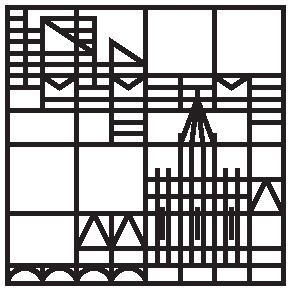
\includegraphics[width=5cm]{logo}
\\ \Large Universität Konstanz  \\ \vspace{4ex} \huge 
Skript zur Vorlesung\\ Höhere Quantentheorie und Elektrodynamik
\\ \vspace{4ex} \Large Prof. Dr. Wolfgang Belzig 
\\ Version vom 30. Juli 2012 \\ \vspace{4.5cm}
\normalsize Ursprünglichen Mitschrift von Birte Heinze im WS 09/10 \\ Ausführliche Überarbeitung von Tobias Lohse im WS 11/12 \vspace{-10cm}}
\author{}
\date{}
\begin{document}

\thispagestyle{empty} 
\maketitle
\thispagestyle{empty}
\newpage
\thispagestyle{empty}
$\;$
\newpage 
\thispagestyle{empty}
$\;$\vspace{3cm}
\par\begingroup\leftskip=3.5cm\rightskip=3.5cm
Dieses Skript basiert auf der Vorlesung von Professor Wolfgang Belzig zur höheren Quantentheorie und Elektrodynamik. Eine Ursprüngliche Mitschrift wurde im Wintersemester 2009/10 von Birte Heinze verfasst und in \LaTeX gesetzt. Im Wintersemester 2011/12 wurde dieses erste Skript von Tobias Lohse komplett überarbeitet und korrigiert und es wurde diese neue Version mit ausführlicheren Texten und überarbeiteten Formeln und Grafiken erstellt. Dieses Skript stellt keine direkte Kopie eines Tafelanschriebs dar, sondern ist mit ausführlicheren Texten und Erklärungen versehen, so dass es den Inhalt der Vorlesung in eigenständiger Weise darbietet. Das Skript ist allerdings keinesfalls ein Ersatz für die Vorlesung und erhebt keinen Anspruch auf Vollständigkeit (oder komplette Fehlerfreiheit) sondern ist als schriftliche Ergänzung zum lernen oder Nachschlagen der Zusammenhänge für Übungsaufgaben gedacht. Der \LaTeX Quelcode ist verfügbar auf https://github.com/MrLoh/QM2Skript, es dürfen gerne Pullrequests gesendet werden.
\par\endgroup 
\newpage 

\setcounter{page}{1}
\thispagestyle{plain}
\tableofcontents
\cleardoublepage 

\pagestyle{fancy}

\thispagestyle{plain} %\documentclass[a4paper,12pt,final,twoside]{scrartcl}
\setcounter{secnumdepth}{3}
\setcounter{tocdepth}{5}

\usepackage[utf8]{inputenc}
\usepackage[T1]{fontenc}
\linespread{1.4}
\usepackage{dsfont}
\usepackage{amsfonts}
\usepackage{amsmath}
\usepackage{amssymb}
\usepackage{amsthm}
\usepackage{mathtools}
\usepackage{mathbbol}
\usepackage{amsmath1}
\usepackage[ngerman]{babel}
\usepackage{bibgerm}
\usepackage[pdftex]{graphicx}
%\usepackage{mathpazo}
\usepackage{floatflt}
%%\usepackage{epsfig}
\usepackage{wrapfig}
\usepackage{graphicx}
\usepackage{tabularx}
\usepackage{caption} 
\usepackage{multicol} 
\usepackage{mathrsfs}
%\usepackage{pspicture}
%\usepackage{eepic}
%\usepackage{epic}
%\usepackage{trfsigns}

%\usepackage[ansinew]{inputenc}
\usepackage{longtable,array,dcolumn}
%\usepackage{ngerman}
\usepackage{epic}
\usepackage{rotate}
\usepackage{graphpap}
\usepackage{amssymb}
\usepackage[squaren]{SIunits}
\usepackage{curves}
\usepackage{float}
\usepackage{array}
\usepackage{enumerate}
\usepackage{marvosym}
\usepackage{slashed}%für feynmanslsash
\usepackage[breaklinks,pdfborder={0 0 0}]{hyperref}
\usepackage{ulem}	%angeblich funktioniert dann
\let\underbar\uline	%underbar in math auch bei greek letters
\usepackage{multirow}
%\usepackage{multicolumn}
\usepackage{enumitem}


\setlength{\parskip}{12pt}
\setlength{\parindent}{0mm}
%\newcommand{\grad}{\ensuremath{^{\circ}}
%\renewcommand{\figurename}{Abb.}		% mit usepackage caption2
%\renewcommand{\captionfont}{\small \itshape}	% mit usepackage caption2
%\setkomafont{caption}{\small \itshape}		%sollte mit caption im userpackage funktionieren
%\setkomafont{captionlabel}{\small , \itshape}	%sollte mit caption im userpackage funktionieren
\captionsetup{font = {small, sf}} %mit it anstelle von sf gibts kusiv

\date{2009-20-10}
\newcommand{\kreis}[1]{
 \qbezier(-#1,0)(-#1,#1)(0,#1)
  \qbezier(0,#1)(#1,#1)(#1,0)
  \qbezier(#1,0)(#1,-#1)(0,-#1)
  \qbezier(0,-#1)(-#1,-#1)(-#1,0)}
\newcommand{\s}{\ \big| \ }
\newcommand{\lo}{\left <}
\newcommand{\ro}{\ri >}
\newcommand{\g}{&=&}

\newcommand{\ham}{\mathcal H}
\newcommand{\hil}{\mathscr H}
\newcommand{\fok}{\mathscr F}
\newcommand{\wh}{\widehat}
%\newcommand{\left}{\left}
\newcommand{\ri}{\right}
\newcommand{\Sp}{\text{Sp}}
\newcommand{\babsatz}{\par \begingroup \leftskip=2cm}
\newcommand{\eabsatz}{\par\endgroup}

\newcommand{\D}{\text{\itshape D}}
\newcommand{\Lr}{\mathcal L }%\textit{L}}
\newcommand{\rot}{\text{rot}}
\newcommand{\divergenz}{\text{div}}
\newcommand{\grad}{\text{grad}}
\newcommand{\grat}{${}^{\circ}$}
%\newcommand{\tanh}{\text{tanh}} already defined

\newcommand{\RM}[1]{\text{\MakeUppercase{\romannumeral #1}}}
\newcommand{\dell}{\partial}
\renewcommand{\div}{\operatorname{div}}
\newcommand{\I}{\dot{\text{\i\!\i}}}
\newcommand{\e}{\mathrm{e}}
\newcommand{\ket}[1]{\mid\!\!\!\,\,{#1}\rangle}
\newcommand{\bra}[1]{\langle{#1}\!\!\!\,\,\mid}
\newcommand{\braket}[2]{\langle{#1}\!\!\!\,\,\mid\!\!\!\,\,{#2}\rangle}
\newcommand{\bracket}[3]{\langle{#1}\!\!\!\,\,\mid\!\!\!\,\,{#2}\!\!\!\,\,\mid\!\!\!\,\,{#3}\rangle}
\newcommand{\1}{\mathds{1}}
\newcommand{\EW}[1]{\langle\!\!\,\,#1\!\!\,\,\rangle}
\newcommand{\arrowbox}[1]{-\!\!\!\!\:\text{(#1)}\!\!\!\;\;\!\!\!\rightarrow}

\newcommand{\ketI}[1]{\ket{#1}_{\!\!\;\text{I}}}
\newcommand{\ketII}[1]{\ket{#1}_{\!\!\;\text{II}}}
\newcommand{\ketIII}[1]{\ket{#1}_{\!\!\;\text{III}}}
\newcommand{\braI}[1]{\,\!_{\text{I}\!\!\;}\bra{#1}}
\newcommand{\braII}[1]{\,\!_{\text{II}\!\!\;}\bra{#1}}
\newcommand{\braketI}[2]{\,_{\text{I}\!\!\;}\braket{#1}{#2}_{\!\!\;\text{I}}\,}
\newcommand{\braketII}[2]{\,_{\text{II}\!\!\;}\braket{#1}{#2}_{\!\!\;\text{II}}\,}
\newcommand{\braketIII}[2]{\,_{\text{III}\!\!\;}\braket{#1}{#2}_{\!\!\;\text{III}}\,}
\newcommand{\bracketI}[3]{\,_{\text{I}\!\!\;}\bracket{#1}{#2}{#3}_{\!\!\;\text{I}}\,}
\newcommand{\bracketII}[3]{\,_{\text{II}\!\!\;}\bracket{#1}{#2}{#3}_{\!\!\;\text{II}}\,}


\newcommand{\up}{\ket{\uparrow}}
\newcommand{\updg}{\bra{\uparrow}}
\newcommand{\down}{\ket{\downarrow}}
\newcommand{\downdg}{\bra{\downarrow}}
\newcommand{\upup}{\ket{\uparrow\uparrow}}
\newcommand{\updown}{\ket{\uparrow\downarrow}}
\newcommand{\downup}{\ket{\downarrow\uparrow}}
\newcommand{\downdown}{\ket{\downarrow\downarrow}}

\newenvironment{itemize1}{\begin{itemize}[leftmargin=5mm,itemsep=-1ex,topsep=-1ex]}{\end{itemize}}

%\usepackage[left=2cm,right=2cm,top=1cm,bottom=1cm,includeheadfoot]{geometry}

\usepackage{fancyhdr}
\pagestyle{fancy}{\fancyhf{}
\fancyhead[LO,RE]{\footnotesize \rightmark}
\fancyfoot[C]{\footnotesize -$\,$\thepage$\;$-}
\renewcommand{\headrulewidth}{0.4pt}
\renewcommand{\footrulewidth}{0pt}}

\fancypagestyle{plain}{\fancyhf{}
\renewcommand{\headrulewidth}{0.4pt}
\fancyfoot[C]{\footnotesize -$\,$\thepage$\,$-}}

\usepackage{titlesec}
\titleformat{\section}[display]{\sffamily\bfseries\Huge\center}{Kapitel \thetitle:}{1ex}{}{}
\newcommand{\kapitel}[2]{$\;$\vspace{-1.5cm} \section[#1]{#2} \rule{17cm}{0.4pt}\vspace{3cm}}
\titleformat{\paragraph}[hang]{\sffamily\bfseries}{\thetitle:}{0ex}{\vspace{-0.15cm}}{\vspace{0.5cm}}

\title{ \vspace{1.5cm}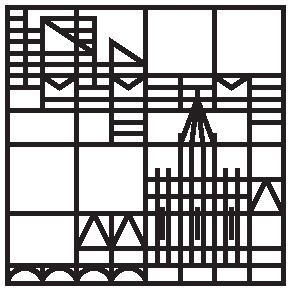
\includegraphics[width=5cm]{logo}
\\ \Large Universität Konstanz  \\ \vspace{4ex} \huge 
Skript zur Vorlesung\\ Höhere Quantentheorie und Elektrodynamik
\\ \vspace{4ex} \Large Prof. Dr. Wolfgang Belzig 
\\ Version vom 30. Juli 2012 \\ \vspace{4.5cm}
\normalsize Ursprünglichen Mitschrift von Birte Heinze im WS 09/10 \\ Ausführliche Überarbeitung von Tobias Lohse im WS 11/12 \vspace{-10cm}}
\author{}
\date{}
%\begin{document}

\subsection*{Einleitung} \vspace{-.5cm}\addcontentsline{toc}{subsection}{\qquad\,\! Einleitung}\markboth{Einleitung}{Einleitung}
Die moderne Quantentheorie stellt heutzutage einen der wichtigsten und umfänglichsten Bereiche der Physik dar, welcher in verschiedensten Bereichen der aktuellen Forschung von Bedeutung ist. In der Tat gibt es nur wenige Bereiche der modernen Physik, in denen Quantenmechanische Effekte keinerlei Rolle spielen. Ein gutes Verständnis der Systematik, mathematischen Formulierung und Anwendung der Quantentheorie ist daher eine absolut notwendige Vorraussetzung für ein Verständnis von moderner Physik. 

Dieses Skript und die Vorlesung auf der es beruht sollen einen Einblick in die Vielfalt der verschiedensten Bereiche der Quantentheorie bieten und eine Grundlage für das Verständnis der Systematik dieser verschiedenen Teilbereiche bieten, auf deren Basis eine Einordnung und ein grundlegendes Verständnis der Teilbereiche moderner Quantenphysik möglich sind. Es werden grundlegende Kenntnisse der klassischen Mechanik, Elektrodynamik und Speziellen Relativitätstheorie sowie der einfachen Quantenmechanik und deren mathematischen Formalismen vorausgesetzt. Der Inhalt ist in Vier Kapitel gegliedert:

\begin{itemize1}
	\item Im ersten Kapitel sollen zunächst die Grundlagen der einfachen Quantenmechanik wiederholt werden, danach soll die Addition von Drehimpulsoperatoren, die zeitabhängige Störungstheorie und die quantenmechanische Streutheorie näher erläutert werden, die in diesen Abschnitten erläuterten Theorien sind insbesondere für das Verständnis der Grundlagen der Festkörperphysik wichtig, spielen aber auch in vielen anderen Anwendungen der Quantenphysik eine wichtige Rolle. Im nächsten Abschnitt soll ein Einblick in die Formulierung und Herleitung der Quantendynamik nach Feynman mittels Propagatoren gegeben werden, welche eine wichtige Grundlage für die Formulierung der Quantenfeldtheorie darstellt. Abschließend soll in diesem ersten Kapitel dann noch kurz auf den Messprozess und die Wahrscheinlichkeitsinterpretation der Quantenmechanik eingegangen werden, welche für das Verständnis von Quantenstatistik und Quanteninformationstheorie eine wichtige Rolle spielen. 
	\item Im zweiten Kapitel soll auf die relativistische Formulierung der Elektrodynamik eingegangen werden. Dazu werden wir zunächst die Grundlagen der Speziellen Relativitätstheorie (SRT) und deren Formalismus wiederholen und danach die Elektrodynamik in diesem Formalismus formulieren. Außerdem soll auf den Lagrangeformalismus der SRT eingegangen werden, welcher die Grundlage für die Formulierung relativistischer Quantenfeldtheorien darstellt. 
	\item Es soll nun im dritten Kapitel auf die Relativistische Quantenmechanik eingegangen werden. Insbesondere sollen die Klein-Gordon-Gleichung und die Dirac-Gleichung Motiviert und Erläutert werden und der Formalismus für die Relativistische Quantenmechanik formuliert werden. Die relativistische Quantenmechanik spielt insbesondere eine bedeutende Rolle, insofern sie den Spin einführt und damit im nichtrelativistischen Grenzfall in die Pauli-Gleichung übergeht. Außerdem stellt sie die Grundalge für jegliche Elementarteilchentheorien dar und motiviert die Notwendigkeit einer Quantenfeldtheorie. 
	\item Im letzten Kapitel soll schlussendlich eine Einführung in die Quantefeldtheorie gegeben werden. Dabei wird zunächst der Formalismus der Quantenfeldtheorie und die Darstellung von Operatoren in zweiter Quantisierung eingeführt. Abschließend soll auf die Feldquantisierung der Diractheorie und des Strahlungsfeldes eingegangen werden. Mit der Quantenfeldheorie ist die Grundlage für die Quantenelektrodynamik und Quantenstatistik und damit  der modernen theoretischen Festkörperphysik gelegt außerdem stellt sie die Grundlage für die Formulierung der Quantenchromodynamik und der gesamten modernen theoretischen Elementarteilchentheorie dar. 
\end{itemize1}

Das folgende Diagramm soll die Zusammenhänge der verschiedenen quantenmechanischen Theorien und die Einordnung in Teilbereiche der Physik verdeutlichen: 

\begin{figure}[b!]\center
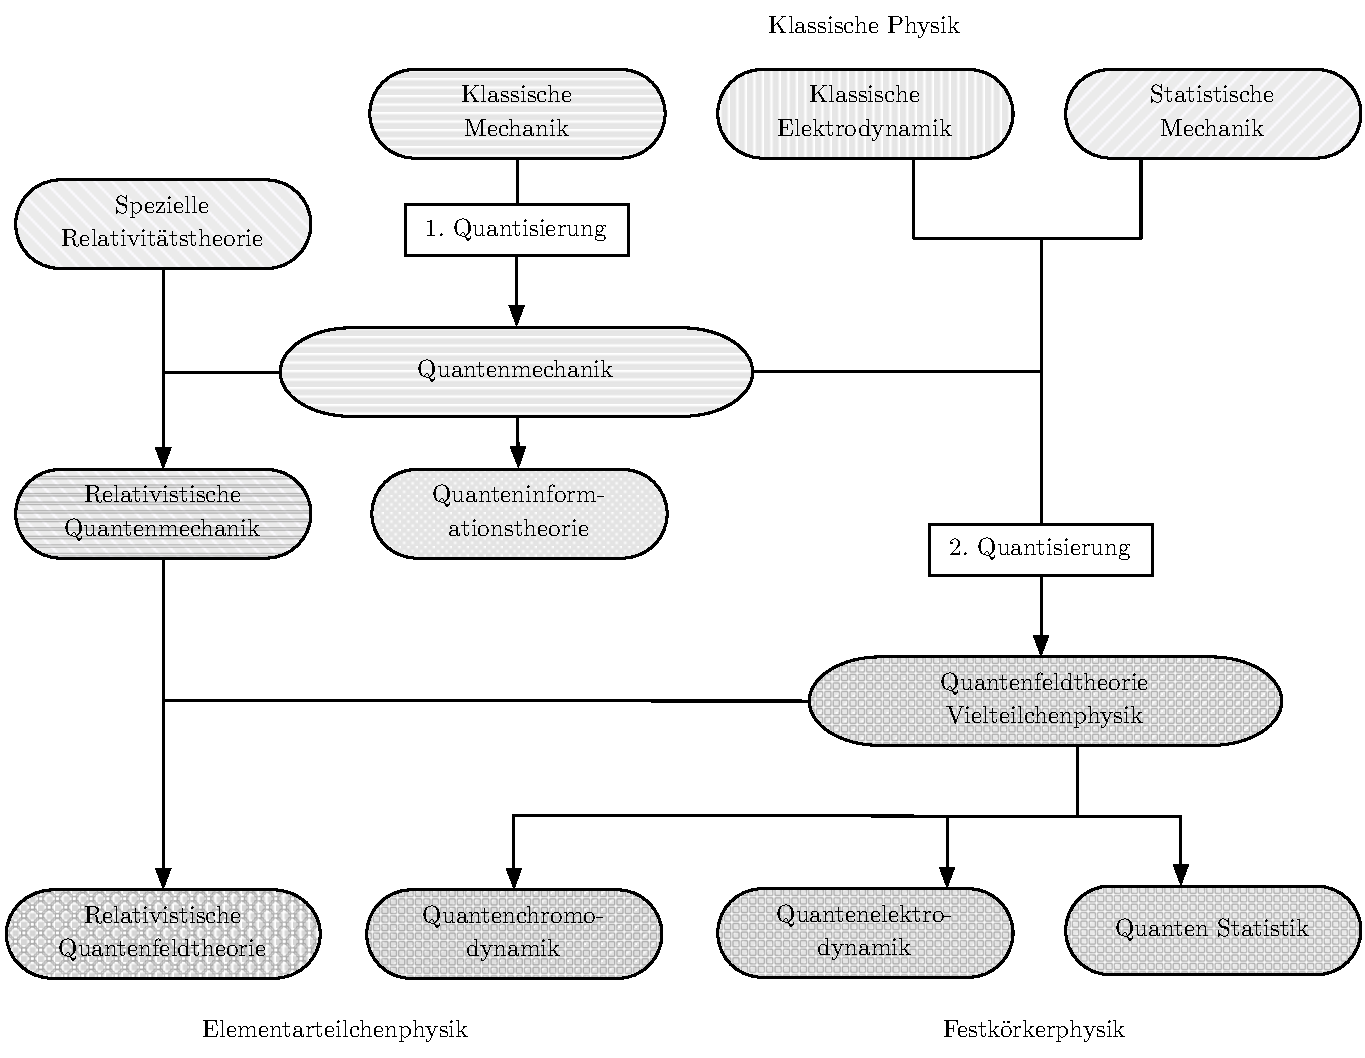
\includegraphics[width=.95\linewidth]{Figs/overview.pdf}
\end{figure}

%\end{document} \newpage 
\thispagestyle{plain}
\kapitel{Nichtrelativistische Quantenmechanik}{Nichtrelativistische \\Quantenmechanik}
\thispagestyle{plain} %\documentclass[a4paper,12pt,final,twoside]{scrartcl}
\setcounter{secnumdepth}{3}
\setcounter{tocdepth}{5}

\usepackage[utf8]{inputenc}
\usepackage[T1]{fontenc}
\linespread{1.4}
\usepackage{dsfont}
\usepackage{amsfonts}
\usepackage{amsmath}
\usepackage{amssymb}
\usepackage{amsthm}
\usepackage{mathtools}
\usepackage{mathbbol}
\usepackage{amsmath1}
\usepackage[ngerman]{babel}
\usepackage{bibgerm}
\usepackage[pdftex]{graphicx}
%\usepackage{mathpazo}
\usepackage{floatflt}
%%\usepackage{epsfig}
\usepackage{wrapfig}
\usepackage{graphicx}
\usepackage{tabularx}
\usepackage{caption} 
\usepackage{multicol} 
\usepackage{mathrsfs}
%\usepackage{pspicture}
%\usepackage{eepic}
%\usepackage{epic}
%\usepackage{trfsigns}

%\usepackage[ansinew]{inputenc}
\usepackage{longtable,array,dcolumn}
%\usepackage{ngerman}
\usepackage{epic}
\usepackage{rotate}
\usepackage{graphpap}
\usepackage{amssymb}
\usepackage[squaren]{SIunits}
\usepackage{curves}
\usepackage{float}
\usepackage{array}
\usepackage{enumerate}
\usepackage{marvosym}
\usepackage{slashed}%für feynmanslsash
\usepackage[breaklinks,pdfborder={0 0 0}]{hyperref}
\usepackage{ulem}	%angeblich funktioniert dann
\let\underbar\uline	%underbar in math auch bei greek letters
\usepackage{multirow}
%\usepackage{multicolumn}
\usepackage{enumitem}


\setlength{\parskip}{12pt}
\setlength{\parindent}{0mm}
%\newcommand{\grad}{\ensuremath{^{\circ}}
%\renewcommand{\figurename}{Abb.}		% mit usepackage caption2
%\renewcommand{\captionfont}{\small \itshape}	% mit usepackage caption2
%\setkomafont{caption}{\small \itshape}		%sollte mit caption im userpackage funktionieren
%\setkomafont{captionlabel}{\small , \itshape}	%sollte mit caption im userpackage funktionieren
\captionsetup{font = {small, sf}} %mit it anstelle von sf gibts kusiv

\date{2009-20-10}
\newcommand{\kreis}[1]{
 \qbezier(-#1,0)(-#1,#1)(0,#1)
  \qbezier(0,#1)(#1,#1)(#1,0)
  \qbezier(#1,0)(#1,-#1)(0,-#1)
  \qbezier(0,-#1)(-#1,-#1)(-#1,0)}
\newcommand{\s}{\ \big| \ }
\newcommand{\lo}{\left <}
\newcommand{\ro}{\ri >}
\newcommand{\g}{&=&}

\newcommand{\ham}{\mathcal H}
\newcommand{\hil}{\mathscr H}
\newcommand{\fok}{\mathscr F}
\newcommand{\wh}{\widehat}
%\newcommand{\left}{\left}
\newcommand{\ri}{\right}
\newcommand{\Sp}{\text{Sp}}
\newcommand{\babsatz}{\par \begingroup \leftskip=2cm}
\newcommand{\eabsatz}{\par\endgroup}

\newcommand{\D}{\text{\itshape D}}
\newcommand{\Lr}{\mathcal L }%\textit{L}}
\newcommand{\rot}{\text{rot}}
\newcommand{\divergenz}{\text{div}}
\newcommand{\grad}{\text{grad}}
\newcommand{\grat}{${}^{\circ}$}
%\newcommand{\tanh}{\text{tanh}} already defined

\newcommand{\RM}[1]{\text{\MakeUppercase{\romannumeral #1}}}
\newcommand{\dell}{\partial}
\renewcommand{\div}{\operatorname{div}}
\newcommand{\I}{\dot{\text{\i\!\i}}}
\newcommand{\e}{\mathrm{e}}
\newcommand{\ket}[1]{\mid\!\!\!\,\,{#1}\rangle}
\newcommand{\bra}[1]{\langle{#1}\!\!\!\,\,\mid}
\newcommand{\braket}[2]{\langle{#1}\!\!\!\,\,\mid\!\!\!\,\,{#2}\rangle}
\newcommand{\bracket}[3]{\langle{#1}\!\!\!\,\,\mid\!\!\!\,\,{#2}\!\!\!\,\,\mid\!\!\!\,\,{#3}\rangle}
\newcommand{\1}{\mathds{1}}
\newcommand{\EW}[1]{\langle\!\!\,\,#1\!\!\,\,\rangle}
\newcommand{\arrowbox}[1]{-\!\!\!\!\:\text{(#1)}\!\!\!\;\;\!\!\!\rightarrow}

\newcommand{\ketI}[1]{\ket{#1}_{\!\!\;\text{I}}}
\newcommand{\ketII}[1]{\ket{#1}_{\!\!\;\text{II}}}
\newcommand{\ketIII}[1]{\ket{#1}_{\!\!\;\text{III}}}
\newcommand{\braI}[1]{\,\!_{\text{I}\!\!\;}\bra{#1}}
\newcommand{\braII}[1]{\,\!_{\text{II}\!\!\;}\bra{#1}}
\newcommand{\braketI}[2]{\,_{\text{I}\!\!\;}\braket{#1}{#2}_{\!\!\;\text{I}}\,}
\newcommand{\braketII}[2]{\,_{\text{II}\!\!\;}\braket{#1}{#2}_{\!\!\;\text{II}}\,}
\newcommand{\braketIII}[2]{\,_{\text{III}\!\!\;}\braket{#1}{#2}_{\!\!\;\text{III}}\,}
\newcommand{\bracketI}[3]{\,_{\text{I}\!\!\;}\bracket{#1}{#2}{#3}_{\!\!\;\text{I}}\,}
\newcommand{\bracketII}[3]{\,_{\text{II}\!\!\;}\bracket{#1}{#2}{#3}_{\!\!\;\text{II}}\,}


\newcommand{\up}{\ket{\uparrow}}
\newcommand{\updg}{\bra{\uparrow}}
\newcommand{\down}{\ket{\downarrow}}
\newcommand{\downdg}{\bra{\downarrow}}
\newcommand{\upup}{\ket{\uparrow\uparrow}}
\newcommand{\updown}{\ket{\uparrow\downarrow}}
\newcommand{\downup}{\ket{\downarrow\uparrow}}
\newcommand{\downdown}{\ket{\downarrow\downarrow}}

\newenvironment{itemize1}{\begin{itemize}[leftmargin=5mm,itemsep=-1ex,topsep=-1ex]}{\end{itemize}}

%\usepackage[left=2cm,right=2cm,top=1cm,bottom=1cm,includeheadfoot]{geometry}

\usepackage{fancyhdr}
\pagestyle{fancy}{\fancyhf{}
\fancyhead[LO,RE]{\footnotesize \rightmark}
\fancyfoot[C]{\footnotesize -$\,$\thepage$\;$-}
\renewcommand{\headrulewidth}{0.4pt}
\renewcommand{\footrulewidth}{0pt}}

\fancypagestyle{plain}{\fancyhf{}
\renewcommand{\headrulewidth}{0.4pt}
\fancyfoot[C]{\footnotesize -$\,$\thepage$\,$-}}

\usepackage{titlesec}
\titleformat{\section}[display]{\sffamily\bfseries\Huge\center}{Kapitel \thetitle:}{1ex}{}{}
\newcommand{\kapitel}[2]{$\;$\vspace{-1.5cm} \section[#1]{#2} \rule{17cm}{0.4pt}\vspace{3cm}}
\titleformat{\paragraph}[hang]{\sffamily\bfseries}{\thetitle:}{0ex}{\vspace{-0.15cm}}{\vspace{0.5cm}}

\title{ \vspace{1.5cm}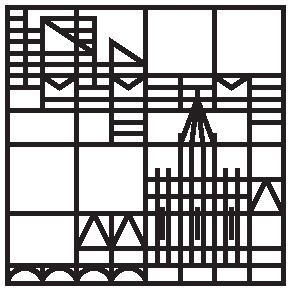
\includegraphics[width=5cm]{logo}
\\ \Large Universität Konstanz  \\ \vspace{4ex} \huge 
Skript zur Vorlesung\\ Höhere Quantentheorie und Elektrodynamik
\\ \vspace{4ex} \Large Prof. Dr. Wolfgang Belzig 
\\ Version vom 30. Juli 2012 \\ \vspace{4.5cm}
\normalsize Ursprünglichen Mitschrift von Birte Heinze im WS 09/10 \\ Ausführliche Überarbeitung von Tobias Lohse im WS 11/12 \vspace{-10cm}}
\author{}
\date{}
%\begin{document}

\setcounter{subsection}{-1}
\subsection{Wiederholung der Grundlagen der Quantenmechanik}
In diesem ersten Abschnitt sollen die wichtigsten Grundlagen der Quantenmechanik wiederholt werden. Diese Darstellung legt dabei weniger Wert auf Vollständigkeit als vielmehr darauf die Formeln und Definitionen zusammen zufassen, welche in den folgenden Abschnitten gebraucht werden. 

\subsubsection{Zustand eines Systems}

Der Zustand eines Systems ist die Gesamtheit der zur vollständigen Beschreibung des Systems minimal erforderlichen Informationen. 

In der analytischen Mechanik ist der Zustand eines Systems zum Zeitpunkt $t$ definiert als Vektor aus generalisierten Koordinaten $\vec{r}(t)$ und Impulsen $\vec{p}(t)$ des Systems zu diesem Zeitpunkt. Der Zustand zum Zeitpunkt $t$ ist also einem Vektor in einem reellen Vektorraum mit Dimension $2N+1$, wobei $N$ die Anzahl der generalisierten Koordinaten ist. Der Zustand im Laufe der Zeit kann als Trajektorie in diesem Vektorraum beschrieben werden. 

In der Quantenmechanik wird der Zustand des Systems zum Zeitpunkt $t$ hingegen als Wellenfunktion $\psi(\vec{r},t)$ in einem {\bf Hilbertraum} $\hil$ beschrieben. Die Dimension und Basis des Hilbertraums wird dabei durch die Randbedingungen des Systems festgelegt. 

Die Wellenfunktion kann in der algebraisch vorteilhaften {\bf Diracnotation} als sogenannter {\bf Ket-Vektor} $\ket{\psi(t)}$ dargestellt werden, die explizite Darstellung der Zeitabhängigkeit wird dabei meist weggelassen. Zu jedem Ket kann ein sogenannter {\bf Bra-Vektor} $\bra{\psi}$ im dualen Raum definiert werden, so dass $\braket{\psi}{\phi}$ das Skalarprodukt zwischen den beiden Kets $\ket{\psi}$ und $\ket{\phi}$ darstellt. Damit kann der Ket-Vektor in der Diracnotation dann wie folgt mit der Wellenfunktion in der {\bf Schrödingernotation} identifiziert werden: 
\begin{eqnarray*}
	\text{Diracnotation: $\ket{\psi(t)}$}\qquad \braket{\vec{r}}{\psi(t)} &=& \psi(\vec{r},t) \qquad\text{Schrödingernotation: $\psi(\vec{r},t)$} 
\end{eqnarray*}

\paragraph{Basis}
Jeder Hilbertraum $\hil$ besitzt eine {\bf orthonormale Basis} (ONB), das heißt eine Anzahl von linear unabängigen Vektoren $[\;(\ket{b_i})_i\;]=\hil$, die orthogonal zu einander und normiert sind: $\braket{b_i}{b_j}=\delta_{ij}$. Jeder Zustand im Hilbertraum lässt sich in einer solchen orthonormalen Basis entwickelnd. Im falle eines endlich dimensionalen Hilbertraums lässt sich dies schreiben als: 
\begin{eqnarray*}
	\ket{\psi} &=& \sum_{i} \underbrace{\braket{b_i}{\psi}}_{=c_i} \ket{b_i}
\end{eqnarray*}
Die Faktoren $c_i$ sind die {\bf Koordinaten} des Vektors $\ket{\psi}$ in der Basis $(\ket{b_i})_i$. In einer endlichen Basis lässt sich der Zustand somit als Spaltenvektor schreiben. Im Falle eines unendlich dimensionalen Hilbertraums, wir die Summe einfach durch ein integral über alle Basisvektoren ersetzt. 

\subsubsection{Wahrscheinlichkeitsinterpretation}

Im Gegensatz zur analytischen Mechanik legt der Zustand in der Quantenmechanik nicht den Ausgang jeglicher Messergebnisse fest, sondern wird als Wahrscheinlichkeit interpretiert. Die Wahrscheinlichkeit am System im Zustand $\ket{\psi}$ ein Teilchen am Ort $\vec{r}$ zur Zeit $t$ zu messen $p_{\vec{r}}(t)$ ist nach der {\bf Bornschen-Wahrscheinlichkeitsinterpretation} gegeben durch: 
\begin{eqnarray*}
	p_{\vec{r}}(t) &=& |\psi(\vec{r},t)|^2 = |\braket{\psi(t)}{\psi(t)}| 
\end{eqnarray*}
Der Zustand muss daher für alle Zeiten normiert werden: 
\begin{eqnarray*}
	|\braket{\psi(t)}{\psi(t)}| = \int \mathrm{d}^3r\; |\psi(\vec{r},t)| &\overset{!}=& 1
\end{eqnarray*}
Die Wahrscheinlichkeitsinterpretation kann für beliebige Messgrößen verallgemeinert werden. Die Wahrscheinlichkeit $p_{m}(t)$ das System im Zustands $\ket{m}$ zu finden ist dann gegeben durch: 
\begin{eqnarray*}
	p_m(t) &=& |\braket{m}{\psi(t)}|^2
\end{eqnarray*}

\subsubsection{Zeitentwicklung und Schrödingergleichung}

Die Zeitentwicklung des Zustandes wird durch die {\bf Schrödingergleichung} beschreiben: 
\begin{equation}
	\I \hbar\; \partial_t \ket{\psi(t)} = \hat{\ham}(\vec{r},t) \ket{\psi(t)}	\label{SG}
\end{equation}
Der {\bf Hamiltonoperator} $\hat{\ham}(\vec{r},t)$ kann mittels des Korrespondenzprinzips aus der Hamiltonfunktion der analytischen Mechanik hergeleitet werden, indem die Koordinaten $r_i$ und ihre konjugierten Impulse $p_i$ kanonisch quantisiert werden. Dies bedeutet, dass die Variablen $r_i$ und $p_i$ als Operatoren $\hat{r}_i$ und $\hat{p}_i$ interpretiert werden, welch die {\bf Vertauschungsrelation} $[\hat{r}_i,\hat{p}_i]=\delta_{ij}\I\hbar$ erfüllen. 

Für ein Teilchen im elektromagnetischen Feld mit Vektorpotential $\vec{ A}(\vec{r},t)$ und skalarem Potential $\phi(\vec{r},t)$ ergibt sich dann beispielsweise folgender Hamiltonoperator:
\begin{eqnarray*}
	\hat{\ham}(\vec{r},t) &=& \frac1{2m} \Big( \hat{\vec{p}} - q\hat{\vec{A}}(\hat{\vec{r}},t)\Big)^2 + q\hat{\phi}(\hat{\vec{r}},t)
\end{eqnarray*}
Das elektrische Feld $\vec{E}$ und das magnetische Feld $\vec{B}$ ergeben sich, ganz normal zu: 
\begin{eqnarray*}
	\vec{E} = -\nabla\phi - \partial_t\vec{A} &\qquad& \vec{B} = \nabla \times \vec{A}
\end{eqnarray*}
Die Ortsoperatoren $\hat{\vec{r}}$ und Implusoperatoren $\hat{\vec{p}}$ ergeben sich aus der kanonischen Vertauschungsrelation im Orts- bzw. Impulsraum wie folgt: 
\begin{eqnarray*}
	\text{Ortsraum:}\qquad \hat{\vec{p}} \;\psi(\vec{r}) &=& -\I\hbar \vec \nabla_{\vec{r}}\;\psi(\vec{r})
	\\
	\text{Impulsraum:}\qquad \hat{\vec{r}} \;\psi(\vec{p}) &=& +\I\hbar \vec \nabla_{\vec{p}}\;\psi(\vec{r})
\end{eqnarray*}

\paragraph{Stationäre Zustände}
Falls die Potentiale $\hat{\phi}$ und $\hat{\vec{A}}$ zeitunabhängig sind, lässt sich mit folgendem Lösungsansatz die Zeitabhängigkeit separieren und es ergibt sich die sogenannte {\bf stationäre Schrödingergleichung}: 
\begin{eqnarray}
	\psi(\vec{r},t) = \e^{-\I\frac{E t}{\hbar}} \cdot \psi(\vec{r}) &\overset{(\ref{SG})}{\Rightarrow}& E \psi(\vec{r}) = \hat{\ham}(\vec{r})\psi(\vec{r}) \label{statSG}
\end{eqnarray}
Die Lösung der Schrödingergleichung reduziert sich damit auf ein Eigenwertproblem. Damit ist die Energie des Systems nicht kontinuierlich, sondern kann nur bestimmte quantisierte Eigenwerte annehmen. 

\subsubsection{Observablen und Operatoren}

Eine Observable ist eine messbarer Parameter des Systems. In der Quantenmechanik werden Observablen nicht als Funktionen der Parameter des Systems geschrieben, sondern als lineare hermitesche Operatoren, welche auf die Zustände des Systems wirken und mittels derer die Wahrscheinlichkeit einer Messung am System bestimmt werden kann. Damit ein Operator eine reelle Messgröße repräsentieren kann muss er die Bedingung der Hermitizität erfüllen: $\hat{A}=\hat{A}^{\dagger}$. 

\paragraph{Spektrum}
Jeder hermitesche Operator $\hat{A}$ kann in einer orthonormalen Basis $(\ket{b_i})_i$ entwickelt werden. In einem endlich dimensionalen Hilbertraum lässt sich dies wie folgt darstellen: 
\begin{eqnarray*}
	\hat{A} &=& \sum_{i,j} \ket{b_i}\underbrace{\bracket{b_j}{\hat{A}}{b_i}}_{= A_{ij}}\bra{b_j} = \sum_{i,j} A_{ij} \ket{b_i}\bra{b_j}
\end{eqnarray*}
Die Faktoren $A_{ij}$ sind dann die Matrixelemente des Operators $\hat{A}$ in der Basis $(\ket{b_i})_i$ und der Operator kann somit als reellwertige Matrix geschrieben werden. In unendlich dimensionalen Hilberträumen muss die Summe durch ein Integral ersetzt werden. 

Für jede Observable lässt sich eine orthonormale Basis finden, in der diese Matrix nur diagonal Elemente hat. Diese Basis wird als Eigenbasis des Operators und die Diagonalenelemente als Spektrum des Operators bezeichnet. Die Darstellung des Operators in seiner Eigenbasis wird auch als {\bf Spektralform} $\hat{A}=\sum_{i}a_i\ket{a_i}\bra{a_i}$ bezeichnet. Ein Element des Spektrum $a_i$ wird auch als {\bf Eigenwert} und das zugehörige Element der Eigenbasis als {\bf Eigenzustand} $\ket{a_i}$ bezeichnet, da sie folgende Eigenwertgleichung erfüllen: 
\begin{eqnarray*}
	\hat{A}\ket{a_i} &=& a_i \ket{a_i}
\end{eqnarray*}
Man spricht davon, dass $a_i$ ein Eigenwert des Operators $\hat{A}$ zum Eigenzustand $\ket{a_i}$ ist. 


\paragraph{Erhaltungsgrößen}

Eine Observable $\hat{A}$ ist eine Erhaltungsgröße des Systems, das heißt eine zeitliche Konstante $\mathrm{d}\EW{\hat{A}}/\mathrm{d}t=0$, genau dann wenn sie mit dem Hamiltonoperator kommutiert, dass bedeutet der {\bf Kommutator} wird 0: $[\hat{\ham},\hat{A}]=\hat{\ham}\hat{A}-\hat{A}\hat{\ham}=0$. 


\subsubsection{Messprozess}

Der {\bf Erwartungswert} der Messung einer Observable $\hat{A}$ am System mit Zustand $\ket{\psi}$ ist gegeben durch: $\EW{\hat{A}}=\bracket{\psi}{\hat{A}}{\psi}$. Der Erwartungswert entspricht dabei dem theoretischen Mittelwert nach beliebig vielen Messungen. Das Ergebnis einer einzelnen Messung hingegen ist immer ein Eigenwert $a_i$ des Operators $\hat{A}$ mit zugehörigem Eigenzustand $\ket{a_i}$. Der Mittelwert selbst ist nicht notwendigerweise ein Eigenwert. Der Erwartungswert einer Observable hat in diesem Sinne keine physikalische, sondern lediglich eine statistische Realität. 

Die Wahrscheinlichkeit $p_{a_i}$ für die Messung des Eigenwerts $a_i$ mit Eigenzustand $\ket{a_i}$ ergibt sich nach der Bornschen-Wahrscheinlichkeitsinterpretation dann zu: $p_{a_i}=|\braket{a_i}{\psi}|^2$

Zwei Observablen $\hat{A}$ und $\hat{B}$ sind nur gleichzeitig messbar, wenn sie gemeinsame Eigenzustände besitzen, was der Falls ist, wenn sie miteinander kommutieren: $[\hat{A},\hat{B}]=0$. 

\paragraph{Projektionspostulat}

Das Projektionspostulat besagt, dass sich das System nach der Messung des einer Observablen im Eigenzustand des gemessenen Eigenwerts befindet: 
\begin{eqnarray*}
	\ket{\psi} \quad\arrowbox{Messung von $a_i$}\quad \ket{a_i}
\end{eqnarray*}
Der Zustand eines Systems wird also durch die Messung in den Eigenzustand projiziert und damit verändert. Dies wird auch als {\bf Kollaps der Wellenfunktion} bezeichnet. Durch die Messung wird der Zustand des Systems somit geändert. In der Quantenmechanik gibt es somit eine weitere Form der Zeitentwicklung mit folgenden Eigenschaften: 

\begin{itemize1}
	\item Die Projektion ist eine nicht unitäre, das heißt unumkehrbar, Zeitentwicklung. 
	\item Bei der Projektion gehen alle Informationen über den Zustand $\ket{\psi}$ vor der Messung verloren.
	\item Nach der Projektion befindet sich das System in einem reinen Zustand, eine wiederholte Messung ergibt somit immer erneut den zuvor gemessenen Eigenwert.
\end{itemize1}


\subsubsection{freies Teilchen}

Für den Fall, dass kein Potential vorhanden ist, $\hat{V}=0$, spricht man von einem freien Teilchen. Der Hamilton Operator ergibt sich dann zu: $\hat{\ham}=\hat{\vec{p}}/2m$. Der Impulsoperator kommutiert offensichtlich mit dem Hamiltonoperator, $[\hat{\ham},\hat{\vec{p}}\,]=0$, und ist somit erhalten. Die Eigenzustände sind somit {\bf ebene Wellen}, die im Ortsraum wie folgt geschrieben werden: 
\begin{eqnarray*}
	\psi_{\vec k}(\vec{r}) &=& C \cdot \e^{\I \vec{k}\vec{r}} \qquad \text{mit: } \hat{\vec{p}}\;\;\psi_{\vec k}(\vec r) = \underbrace{\hbar\vec{k}}_{=\vec{p}}\psi_{\vec k}(\vec r)
\end{eqnarray*}
Die Energie-Eigenwerte $E_{\vec{k}}$ des Hamiltonoperators ergeben sich somit zu: $E_{k}=\hbar^2k^2/2 m=\hbar\omega_k$. Damit ergibt sich die Zeitentwicklung des Zustandes zu: $\psi_{\vec{k}}(\vec{r},t) = C\cdot\e^{\I(\vec{k}\vec{r}-\omega_kt)}$. 

Die allgemeine Lösung ist eine Überlagerung dieser ebenen Wellen in einem Wellenpaket: 
\begin{eqnarray*}
	\psi(\vec{r},t) &=& \int \mathrm{d}^3k\; C(\vec{k})\cdot\e^{\I\big(\vec{k}\vec{r}-\omega(k)t\big)} \qquad\text{mit: }\omega(k) = \frac{E(k)}{\hbar} = \frac{\hbar k^2}{2m}
\end{eqnarray*}


\subsubsection{Harmonischer Oszillator}

Für ein quadratisches Potential: $\hat{V} = m/2\cdot\omega^2 \hat{x}^2$, ergibt sich der Hamilton Operator des harmonischen Oszillators zu:
\begin{eqnarray*}
\hat \ham = \frac{\hat{p}^2}{2m} + \frac12 m\omega^2 \hat{x}^2
\end{eqnarray*}
Zur Lösung der Schrödingergleichung des harmonischen Oszillators nach der sogenannte Dirac-Methode, führen wir zunächst einheitenlose Koordinaten $\hat{P}=\hat{p}\cdot\hbar\ell$ und $\hat{X}=\hat{x}/\ell$ ein, wobei $\ell=\sqrt{m\omega/\hbar}$ die sogenannte Oszillator-Länge ist. Damit lässt sich der Hamiltonoperator dann wie folgt schreiben: 
\begin{eqnarray*}
	\hat{\ham} = \frac{\hbar\omega}{2} (\hat{P}^2+\hat{X}^2) \quad\text{mit: } \hat{P}=\sqrt{\hbar m\omega}\cdot\hat{p}\text{,  }\hat{X}=\sqrt{\frac {\hbar}{m \omega}}\cdot\hat{x} \text{,  }[\hat{X}, \hat{P}]=\I
\end{eqnarray*}
Es können nun der sogenannte {\bf Aufsteigeoperator} $\hat{a}^{\dagger}$ und der sogenannte {\bf Absteigeoperator} $\hat{a}$ definiert werden:
\begin{eqnarray*}
	\hat{a}=\frac1{\sqrt{2}}\cdot(\hat{X}+\I\hat{P}) &\quad& \hat{a}^{\dagger} = \frac1{\sqrt2}\cdot(\hat{X}-\I \hat{P})
\end{eqnarray*}
Der Kommutator ergibt sich zu: $[\hat{a},\hat{a}^{\dagger}]=1$. Außerdem wird noch der sogenannte {\bf Anzahloperator} $\hat{n}=\hat{a}^{\dagger}\hat{a}$ definiert, so dass sich der Hamiltonoperator einfach schreiben lässt und man direkt sieht, dass die Eigenzustände des Hamiltonoperators mit Eigenenergy $E_n$ die Eigenzustände $\ket{n}$ des Anzahloperators sind:
\begin{eqnarray*}
	\hat{\ham}=\hbar\omega\cdot\Big(\hat{n}+\frac12\Big) &\Rightarrow& \hat{\ham}\ket{n}=\underbrace{\hbar\omega\Big(n+\frac12\Big)}_{=E_n}\ket{n}
\end{eqnarray*}
Es lässt sich zeigen, dass die Eigenwerte des Anzahloperators die natürlichen Zahlen $n\in\mathbb{N}$ sind. Somit sieht man, dass der Anzahloperator angibt, in der wievielten Anregungen $E_n$ des Oszillators sich das System befindet. Außerdem lässt sich nun zeigen, dass die Auf- und Absteigeoperatoren tatsächlich die Anregung um ein Niveau anheben, beziehungsweise absenken: 
\begin{eqnarray*}
	\hat{a}^{\dagger}\ket{n} = \sqrt{n+1}\ket{n+1} &\qquad&\hat{a}\ket{n} = \sqrt{n}\ket{n-1}
\end{eqnarray*}
Der harmonische Oszillator ist eines wichtigsten Modelle in der Quantenmechanik, welches vielseitige Anwendungen in der Modellbildung und verschiedenen Näherungen hat. 


\subsubsection{Zentralpotential und Drehimpulsoperator}

Ein weiteres wichtiges Modellsystem in der Quantenmechanik ist ein Zentralpotential $V(\vec{r})=V(r)$, in welchen - wie wir aus der klassischen Mechanik wissen - der Bahndrehimpuls erhalten ist. Ein typisches Beispiel für ein solches System ist das Wasserstoffatom. 

Der Bahndrehimpulsoperator $\hat{\vec{L}}$ kann ganz 'normal' als Kreuzprodukt aus Impulsoperator $\hat{\vec{p}}$ und Ortsoperator $\hat{\vec{r}}$ definiert werden: $\hat{\vec{L}}=\hat{\vec{r}} \times \hat{\vec{p}}$. Es lässt sich leicht zeigen, dass für ein Zentralpotential der Drehimpulsoperator mit dem Hamiltonoperator $\hat{\ham}(\hat{\vec{r}},\hat{\vec{p}})=\hat{\ham}(\hat{r},\hat{\vec{p}})$ kommutiert $[\hat{\vec{L}},\hat{\ham}]=0$, der Drehimpuls ist also auch in der Quantenmechanik eine Erhaltungsgröße. 


\paragraph{Eigenschaften von Drehimpulsoperatoren}
Das Konzept des Drehimpulses in der Quantenmechanik kann verallgemeinert werden. Der Drehimpulsoperator ist durch eine spezifische Algebra ausgezeichnet, die als {\bf Drehimpulsalgebra} bezeichnet und durch folgende Bedingung beschrieben wird: 
\begin{eqnarray}
	[\hat{L}_i, \hat{L}_j] = \I\hbar\sum_{k=1}^{3} \varepsilon_{ijk} \hat{L}_k &\quad\Leftrightarrow\quad& \hat{\vec{L}} \times \hat{\vec{L}} = \I\hbar \hat{\vec{L}}	\label{Drehimpulsalgebra}
\end{eqnarray}
Jeder Satz von drei Operatoren, für die die Drehimpulsalgebra (\ref{Drehimpulsalgebra}) gilt, wird als quantenmechanischer Drehimpuls behandelt. Ein wichtiges Beispiel für einen anderen solchen Operator in der Quantenmechanik ist der Spinoperator $\hat{\vec{S}}$. 

Ein Drehimpulsoperator $\hat{\vec{L}}=\sum_{i\in\{x,y,z\}}\hat{L}_i \vec{e}_i$ hat einige wichtige Eigenschaften, auf die im folgenden eingegangen werden soll: 
\begin{itemize1}
	\item Der Drehimpulsbetragsoperator, beziehungsweise sein Quadrat $\hat{L}^2=\sum_{i\in\{x,y,z\}}\hat{L}_i^2$ kommutiert mit jeder Komponente des Drehimpulsoperators: 
	\begin{eqnarray*}
		[\hat{L}^2,\hat{L}_i] &=& 0 \qquad\forall i\in\{x,y,z\}
	\end{eqnarray*}
	\item Das Spektrum des Drehimpulsoperators lässt sich in der orthonormalen Basis der $\ket{m,l}$ entwickeln, welche folgende Eigenwertgleichungen erfüllen: 
	\begin{eqnarray*}
		\hat{L}^2 \ket{m,l} = \hbar^2\cdot l(l+1) \ket{m,l} &\quad\land\quad& \hat{L}_z \ket{m,l} = \hbar m\ket{m,l}
	\end{eqnarray*}
	Aus der Algebra folgt $l\in\{n/2\;\big|\; n\in\mathbb{N}\}$ und $m\in\{-l+n\;\big|\; n\in\mathbb{N}\land n\leq 2l\}$. Die Eigenwerte $m$ und $l$ sind somit quantisiert und werden auch als Quantenzahlen bezeichnet. Für jeden Zustand $\ket{l}$ lassen sich somit $2l+1$ Eigenzustände von $\hat{L}_z$ finden, man spricht davon, dass $\ket{l}$ $2l+1$-fach entartet ist. 
	\item Für die diskreten Zustände $\ket{l,m}$ können die  {\bf Leiteroperatoren} $\hat{L}^{\pm} = \hat{L}_x \pm \I\hat{L}_y$ definiert werden. Aus der Drehimpulsalgebra lässt sich folgern, dass gilt: 
	\begin{eqnarray*}
		[\hat{L}_z,\hat{L}^{\pm}] = \pm\hbar\;\hat{L}^{\pm} &\quad\land\quad& [\hat{L}^+,\hat{L}^-] = 2\hbar\;\hat{L}_z
	\end{eqnarray*}
	Daraus und aus der Normierung folgt dann die Wirkung auf die Eigenzustände: 
	\begin{eqnarray*}
		\hat{L}^{\pm}\ket{l,m} = \hbar \underbrace{\sqrt{l(l+1)-m(m\pm1)}}_{=a_{l,m}^{\pm}}\ket{l,m\pm1}
	\end{eqnarray*}
	Wegen $\hat{L}^+\ket{l,l}=0$ und $\hat{L}^-\ket{l,-l}=0$ ist dann sofort ersichtlich, dass $\ket{l,l}$ der maximale Zustand und $\ket{l,-l}$ der minimaler Zustand des Systems ist. 
\end{itemize1}

Ein klassisches Beispiel für ein Zentralpotential ist das Wasserstoffatom, dessen quantisierte Atomorbitale sich aus den Eigenschaften des Bahndrehimpulsoperators erklären lassen. Der Bahndrehimpuls $\hat{\vec{L}}$ der Wasserstoff-Elektronen kann ganzzahlige Werte für $l$ annehmen. Die Eigenzustände des Bahdrehimpulses sind die Kugelflächenfunktionen. 

Neben dem Bahndrehimpuls spielt in der Quantenmechanik der Spin $\hat{\vec{S}}$ - auch Eigendrehimpuls genannt - eine wichtige Rolle, welcher ebenfalls die Drehimpulsalgebra erfüllt. Dieser kann halbzahlige Werte annehemen und ist eine Eigenschaft eines jeden Teilchens, welche sich mittels relativistischer Quantenmechanik (siehe Kapitel 4) erklären lässt. 

Der Gesamtdrehimpuls $\hat{\vec{J}}$ eines Teilchen ist die Summe aus Bahndrehimpuls und Spin: $\hat{\vec{J}} = \hat{\vec{L}} + \hat{\vec{S}}$. 


%\end{document} \newpage 
\thispagestyle{plain} %\documentclass[a4paper,12pt,final,twoside]{scrartcl}
\setcounter{secnumdepth}{3}
\setcounter{tocdepth}{5}

\usepackage[utf8]{inputenc}
\usepackage[T1]{fontenc}
\linespread{1.4}
\usepackage{dsfont}
\usepackage{amsfonts}
\usepackage{amsmath}
\usepackage{amssymb}
\usepackage{amsthm}
\usepackage{mathtools}
\usepackage{mathbbol}
\usepackage{amsmath1}
\usepackage[ngerman]{babel}
\usepackage{bibgerm}
\usepackage[pdftex]{graphicx}
%\usepackage{mathpazo}
\usepackage{floatflt}
%%\usepackage{epsfig}
\usepackage{wrapfig}
\usepackage{graphicx}
\usepackage{tabularx}
\usepackage{caption} 
\usepackage{multicol} 
\usepackage{mathrsfs}
%\usepackage{pspicture}
%\usepackage{eepic}
%\usepackage{epic}
%\usepackage{trfsigns}

%\usepackage[ansinew]{inputenc}
\usepackage{longtable,array,dcolumn}
%\usepackage{ngerman}
\usepackage{epic}
\usepackage{rotate}
\usepackage{graphpap}
\usepackage{amssymb}
\usepackage[squaren]{SIunits}
\usepackage{curves}
\usepackage{float}
\usepackage{array}
\usepackage{enumerate}
\usepackage{marvosym}
\usepackage{slashed}%für feynmanslsash
\usepackage[breaklinks,pdfborder={0 0 0}]{hyperref}
\usepackage{ulem}	%angeblich funktioniert dann
\let\underbar\uline	%underbar in math auch bei greek letters
\usepackage{multirow}
%\usepackage{multicolumn}
\usepackage{enumitem}


\setlength{\parskip}{12pt}
\setlength{\parindent}{0mm}
%\newcommand{\grad}{\ensuremath{^{\circ}}
%\renewcommand{\figurename}{Abb.}		% mit usepackage caption2
%\renewcommand{\captionfont}{\small \itshape}	% mit usepackage caption2
%\setkomafont{caption}{\small \itshape}		%sollte mit caption im userpackage funktionieren
%\setkomafont{captionlabel}{\small , \itshape}	%sollte mit caption im userpackage funktionieren
\captionsetup{font = {small, sf}} %mit it anstelle von sf gibts kusiv

\date{2009-20-10}
\newcommand{\kreis}[1]{
 \qbezier(-#1,0)(-#1,#1)(0,#1)
  \qbezier(0,#1)(#1,#1)(#1,0)
  \qbezier(#1,0)(#1,-#1)(0,-#1)
  \qbezier(0,-#1)(-#1,-#1)(-#1,0)}
\newcommand{\s}{\ \big| \ }
\newcommand{\lo}{\left <}
\newcommand{\ro}{\ri >}
\newcommand{\g}{&=&}

\newcommand{\ham}{\mathcal H}
\newcommand{\hil}{\mathscr H}
\newcommand{\fok}{\mathscr F}
\newcommand{\wh}{\widehat}
%\newcommand{\left}{\left}
\newcommand{\ri}{\right}
\newcommand{\Sp}{\text{Sp}}
\newcommand{\babsatz}{\par \begingroup \leftskip=2cm}
\newcommand{\eabsatz}{\par\endgroup}

\newcommand{\D}{\text{\itshape D}}
\newcommand{\Lr}{\mathcal L }%\textit{L}}
\newcommand{\rot}{\text{rot}}
\newcommand{\divergenz}{\text{div}}
\newcommand{\grad}{\text{grad}}
\newcommand{\grat}{${}^{\circ}$}
%\newcommand{\tanh}{\text{tanh}} already defined

\newcommand{\RM}[1]{\text{\MakeUppercase{\romannumeral #1}}}
\newcommand{\dell}{\partial}
\renewcommand{\div}{\operatorname{div}}
\newcommand{\I}{\dot{\text{\i\!\i}}}
\newcommand{\e}{\mathrm{e}}
\newcommand{\ket}[1]{\mid\!\!\!\,\,{#1}\rangle}
\newcommand{\bra}[1]{\langle{#1}\!\!\!\,\,\mid}
\newcommand{\braket}[2]{\langle{#1}\!\!\!\,\,\mid\!\!\!\,\,{#2}\rangle}
\newcommand{\bracket}[3]{\langle{#1}\!\!\!\,\,\mid\!\!\!\,\,{#2}\!\!\!\,\,\mid\!\!\!\,\,{#3}\rangle}
\newcommand{\1}{\mathds{1}}
\newcommand{\EW}[1]{\langle\!\!\,\,#1\!\!\,\,\rangle}
\newcommand{\arrowbox}[1]{-\!\!\!\!\:\text{(#1)}\!\!\!\;\;\!\!\!\rightarrow}

\newcommand{\ketI}[1]{\ket{#1}_{\!\!\;\text{I}}}
\newcommand{\ketII}[1]{\ket{#1}_{\!\!\;\text{II}}}
\newcommand{\ketIII}[1]{\ket{#1}_{\!\!\;\text{III}}}
\newcommand{\braI}[1]{\,\!_{\text{I}\!\!\;}\bra{#1}}
\newcommand{\braII}[1]{\,\!_{\text{II}\!\!\;}\bra{#1}}
\newcommand{\braketI}[2]{\,_{\text{I}\!\!\;}\braket{#1}{#2}_{\!\!\;\text{I}}\,}
\newcommand{\braketII}[2]{\,_{\text{II}\!\!\;}\braket{#1}{#2}_{\!\!\;\text{II}}\,}
\newcommand{\braketIII}[2]{\,_{\text{III}\!\!\;}\braket{#1}{#2}_{\!\!\;\text{III}}\,}
\newcommand{\bracketI}[3]{\,_{\text{I}\!\!\;}\bracket{#1}{#2}{#3}_{\!\!\;\text{I}}\,}
\newcommand{\bracketII}[3]{\,_{\text{II}\!\!\;}\bracket{#1}{#2}{#3}_{\!\!\;\text{II}}\,}


\newcommand{\up}{\ket{\uparrow}}
\newcommand{\updg}{\bra{\uparrow}}
\newcommand{\down}{\ket{\downarrow}}
\newcommand{\downdg}{\bra{\downarrow}}
\newcommand{\upup}{\ket{\uparrow\uparrow}}
\newcommand{\updown}{\ket{\uparrow\downarrow}}
\newcommand{\downup}{\ket{\downarrow\uparrow}}
\newcommand{\downdown}{\ket{\downarrow\downarrow}}

\newenvironment{itemize1}{\begin{itemize}[leftmargin=5mm,itemsep=-1ex,topsep=-1ex]}{\end{itemize}}

%\usepackage[left=2cm,right=2cm,top=1cm,bottom=1cm,includeheadfoot]{geometry}

\usepackage{fancyhdr}
\pagestyle{fancy}{\fancyhf{}
\fancyhead[LO,RE]{\footnotesize \rightmark}
\fancyfoot[C]{\footnotesize -$\,$\thepage$\;$-}
\renewcommand{\headrulewidth}{0.4pt}
\renewcommand{\footrulewidth}{0pt}}

\fancypagestyle{plain}{\fancyhf{}
\renewcommand{\headrulewidth}{0.4pt}
\fancyfoot[C]{\footnotesize -$\,$\thepage$\,$-}}

\usepackage{titlesec}
\titleformat{\section}[display]{\sffamily\bfseries\Huge\center}{Kapitel \thetitle:}{1ex}{}{}
\newcommand{\kapitel}[2]{$\;$\vspace{-1.5cm} \section[#1]{#2} \rule{17cm}{0.4pt}\vspace{3cm}}
\titleformat{\paragraph}[hang]{\sffamily\bfseries}{\thetitle:}{0ex}{\vspace{-0.15cm}}{\vspace{0.5cm}}

\title{ \vspace{1.5cm}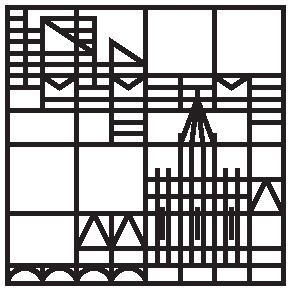
\includegraphics[width=5cm]{logo}
\\ \Large Universität Konstanz  \\ \vspace{4ex} \huge 
Skript zur Vorlesung\\ Höhere Quantentheorie und Elektrodynamik
\\ \vspace{4ex} \Large Prof. Dr. Wolfgang Belzig 
\\ Version vom 30. Juli 2012 \\ \vspace{4.5cm}
\normalsize Ursprünglichen Mitschrift von Birte Heinze im WS 09/10 \\ Ausführliche Überarbeitung von Tobias Lohse im WS 11/12 \vspace{-10cm}}
\author{}
\date{}
%\begin{document}

\subsection{Addition von Drehimpulsen}

In manchen Systemen ist der Gesamtdrehimpuls, welcher als Summe aus Bahndrehimpuls und Spin oder Summe aus den Spins oder Gesamtdrehimpulsen mehrerer Teilchen definiert ist, eine wichtige Größe. Es ist daher hilfreich die Addition von zwei allgemeinen Drehimpulsoperatoren $\hat{\vec{J}}_1$ und $\hat{\vec{J}}_2$ näher zu untersuchen. Der {\bf Gesamtdrehimpuls} $\hat{\vec{J}}$ ist gegeben durch: 
\begin{eqnarray*}
\hat{\vec{J}} &=& \hat{\vec{J}}_1+\hat{\vec{J}}_2
\end{eqnarray*}
Die Drehimpulsoperatoren $\hat{\vec{J}}_1$ und $\hat{\vec{J}}_2$ erfüllen die Drehimpulsalgebra (\ref{Drehimpulsalgebra}) und vertauschen Komponentenweise untereinander aber nicht mit dem Gesamtdrehimpulsquadrat $\hat{J}^2$: 
\begin{eqnarray*}
	\big[\hat{J}_{1i},\hat{J}_{2j}\big] &=& 0 \qquad \forall i\neq j \qquad i,j\in\{x,y,z\}
	\\
	\big[\hat{J}_{1/2\;i},\hat{J}^2\big] &\neq& 0 \qquad \forall i\neq j \qquad \text{mit: } \hat{J}^2=\hat{J}_1^2+\hat{J}_2^2+2\cdot\hat{\vec{J}}_1\cdot\hat{\vec{J}}_2
\end{eqnarray*}
Dies bedeutet, dass wir zwar eine orthonormale Basis mit Produktzuständen $\ket{j_1,m_1}_{\hil_1}\;\oplus\\\ket{j_2,m_2}_{\hil_2}=\;\ket{j_1,j_2,m_1,m_2}_{\hil_1\oplus\hil_2}$ der beiden Drehimpulsoperatoren $\hat{\vec{J}}_1$ und $\hat{\vec{J}}_2$ finden, diese allerdings nicht orthogonal zu den Eigenzuständen des Gesamtdrehimpulses $\ket{j,m}$ sind. 

Dieser Umstand ist relevant für die Erklärung, der Spin-Bahn-Kopplung in Atomen (welche sich allerdings nur mittels relativistischer Quantenmechanik erklären lässt) und der Bandstruktur von Festkörpern und damit insbesondere Halbleitern. 


\subsubsection{Addition von zwei Spin 1/2-Operatoren}

Wir wollen die Addition von Drehimpulsen zunächst am Beispiel zweier Spin 1/2-Operatoren $\hat{\vec{S}}_1$ und $\hat{\vec{S}}_2$ untersuchen. Diese beiden Operatoren sollen wie gesagt komponentenweise miteinander vertauschen und die Drehimplusalgebra erfüllen. Die möglichen Zustände der beiden Teilsysteme $\ket{s_i,m_i}$ sind dann wie wir wissen $s = 1/2$ und $m = \pm 1/2$, die beiden Teilhilberträume $\hil_i$ sind also nur zweidiagonal. Wir führen die übliche abkürzende Schreibweise für die beiden Basiszustände ein: 
\begin{eqnarray*}
	\ket{1/2,+1/2} &=:& \up \qquad\text{wird als 'spin up' bezeichnet}
	\\
	\ket{1/2,-1/2} &=:& \down \qquad\text{wird als 'spin down' bezeichnet}
\end{eqnarray*}
Der Produktraum der beiden Spin-Systeme besitzt dann die vier folgenden Basiszustände:
\begin{eqnarray*}
	\up_{\hil_1}\;\oplus\up_{\hil_2} =\;\upup &\qquad& \down_{\hil_1}\;\oplus\down_{\hil_2} =\;\downdown
	\\
	\up_{\hil_1}\;\oplus\down_{\hil_2} =\;\updown &\qquad& \down_{\hil_1}\;\oplus\up_{\hil_2} =\;\downup
\end{eqnarray*}
Im folgenden werden wir Planck-Einheiten verwenden, also $\hbar=1$ setzen. Der Gesamtspin $\hat{\vec{S}}=\hat{\vec{S}}_1 + \hat{\vec{S}}_2$ erfüllt ebenfalls die Drehimpulsalgebra und seine Eigenzustände haben damit auch die Form $\ket{s,m}$. Wobei die Quantenzahl $m$ den Gesamtdrehimpuls in $z$-Richtung angibt: $\hat{S}_z = \hat{S}_{1z} + \hat{S}_{2z}$. Es sollen also nun die möglichen Werte für $s$ und $m$ bestimmt werden. Dazu untersuchen wir zunächst die Wirkung des Operators $\hat{S}_z$ auf die Basiszustände $\ket{s_1,m_1,s_2,m_2}=\ket{\uparrow\!\!/\!\!\downarrow\;\uparrow\!\!/\!\!\downarrow}$: 
\begin{eqnarray*}
	\hat{S}_z \upup = (\hat{S}_{1z} + \hat{S}_{2z})\upup = \Big(\frac12+\frac12\Big)\upup &=& +1\cdot\upup
	\\
	\hat{S}_z \updown/\downup = \Big(\pm\frac12\mp\frac12\Big)\updown/\downup &=& 0\cdot\updown/\downup
	\\
	\hat{S}_z \downdown = \Big(-\frac12-\frac12\Big)\downdown &=& -1\cdot\downdown 
\end{eqnarray*}
Die Werte von $m$ sind somit ganzzahlig und nehmen werte zwischen $-1$ und $+1$ an.

Nun wollen wir die Werte für $s$ bestimmen, indem wir die Wirkung des Opeators $\hat{\vec{S}}^{\;2}$ untersuchen. Diesen schreiben wir dazu zunächst wie folgt: 
\begin{eqnarray*}
	\hat{S}^2 &=& \hat{S}_1^2 + \hat{S}_2^2 + 2\cdot\hat{\vec{S}}_1\cdot\hat{\vec{S}}_2 = \hat{S}_1^2 + \hat{S}_2^2 + 2\hat{S}_{1z}\hat{S}_{2z} +2 \hat{S}_{1x} \hat{S}_{2x} + 2\hat{S}_{1y}\hat{S}_{2y} 
	\\
	&=& \hat{S}_1^2 + \hat{S}_2^2 + 2\hat{S}_{1z}\hat{S}_{2z}+S^{+}_1S^{-}_2 + S^{-}_1 S^+_2
\end{eqnarray*}
Für den Spin 1/2 gilt nun $\hat{S}_{1/2}^2\up/\down = 1/2\cdot(1/2+1) \up/\down = 3/4 \up/\down$. Und somit ergibt sich für die Wirkung des Operators $\hat{S}^2$ auf den Zustand $\upup$ folgendes: 
\begin{eqnarray*}
	&& \hat{S}^2 \upup = \Big(\frac34+\frac34+2\cdot\frac12\cdot\frac12+0+0\Big) \upup = 2\cdot \upup = 1\cdot(1+1) \upup \;\overset!=\; s(s+1) \upup 
	\\
	&\Rightarrow& \upup \;=\; \ket{s=1,m=1}
\end{eqnarray*}
Auf die selbe Weise können wir den Zustand $\downdown$ als $\ket{s=1,m=-1}$ identifizieren. 
 
Um den Zustand $\ket{s=1,m=0}$ zu bestimmen, verwenden wir den Operator $\hat{S}^-=\hat{S}_1^-+\hat{S}_2^-$, dessen Wirkung auf $\ket{s,m}$ wir kennen: $\hat{S}^-\ket{s,m}=\sqrt{s(s+1)-m(m-1)}\ket{s,m-1}$. Somit ergibt sich: 
\begin{eqnarray*}
	&&\hat{S}^-\upup = (\hat{S}_1^-+\hat{S}_2^-)\upup = \downup+\updown \quad=\quad \hat{S}^-\ket{1,1} = \sqrt2 \ket{1,0}
	\\
	&\Rightarrow& \ket{1,0} \;=\; \frac1{\sqrt2}\cdot(\updown+\downup)
\end{eqnarray*}
Der letzte Basiszustand $\ket{s=0,m=0}$ ergibt sich unter Ausnutzung der Orthogonalitäts-Bedingung dann als $1/\sqrt2\cdot(\updown-\downup)$. 

Die Eigenzustände von $\hat{S}^2$ und $\hat{S}_z$ werden abhängig vom Wert der Gesamtspinquantenzahl in zwei Gruppen eingeteilt: 
\begin{itemize1}
	\item Den sogenannten {\bf Singulet} Zustand: 
	\\$\ket{0,0}=1/\sqrt2\cdot(\updown-\downup)$
	\item Und die sogenannten {\bf Triplet} Zustände: 
	\\$\ket{1,0}=1/\sqrt2\cdot(\updown-\downup)$
	\\$\ket{1,1}=\upup$
	\\$\ket{1,-1}=\downdown$
\end{itemize1}



\subsubsection{Addition von zwei allgemeinen Drehimpulsoperatoren}

Wir wollen nun den Fall zweier allgemeiner Drehimpulsoperatoren $\hat{\vec{J}}_1$ und $\hat{\vec{J}}_2$ betrachten. Diese vertauschen wie bereits beschrieben Komponentenweise untereinander und erfüllen die Drehimpulsalgebra. Wir werden auch hier im folgenden Planck-Einheiten $\hbar=1$ verwenden. 

In einen Raum indem ein Drehimpulsoperator definiert werden kann, lässt sich für den Teilraum, welcher die Drehimpulssymmetrie beschreibt, eine vollständige orthonormale Basis immer in Eigenzuständen des Operators des Drehimpulsbetrags $\hat{J}_i^2\ket{j_i,m_i}=j_i(j_i+1)\ket{j_i,m_i}$ und des Operators des Drehimpluses in $z$-Richtung $\hat{J}_{iz}\ket{j_i,m_i}=m_i\ket{j_i,m_i}$ beschreiben. Als Basis des Produktraums, indem beide Drehimpulsoperatoren definiert sind, können wir dann folgende Zustände wählen: $\ket{j_1,m_1}_{\hil_1}\;\oplus\ket{j_2,m_2}_{\hil_2}=\ket{j_1,j_2,m_1,m_2}$. 

Der Gesamtdrehimpuls ergibt sich aus der Addition der beiden Drehimpulse $\hat{\vec{J}}=\hat{\vec{J}}_1+\hat{\vec{J}}_2$ und erfüllt damit ebenso die Drehimpulsalgebra (\ref{Drehimpulsalgebra}). Damit gibt es eine weitere Basis mit Eigenzuständen des Operators des Gesamtdrehimpulsbetrags $\hat{J}^2\ket{j,m}=j(j+1)\ket{j,m}$ und des Operators des Gesamtdrehimpulses in $z$-Richtung $\hat{J}_z\ket{j,m}=m\ket{j,m}$. Da der Gesamtdrehimpulsbetrag mit den einzelnen Drehimpulsbeträgen vertauscht $[\hat{J}^2,\hat{J}_{1/2}^2]=0$, ist eine weitere vollständige orthonormale Basis des Systems durch die Zustände $\ket{j_1,j_2,j,m}$ gegeben. 

Da der Operator des Gesamtdrehimpulsbetrags jedoch nicht mit den Operatoren der einzelnen Drehimpulse in $z$-Richtung vertauscht, sind die Basiszustände $\ket{j_1,j_2,m_1,m_2}$ und $\ket{j_1,j_2,j,m}$ nicht identisch. Wir suchen daher die Koordinaten der Eigenzustände der letzteren Darstellung in der ersten Darstellung: 
\begin{eqnarray*}
	\ket{j_1,j_2,j,m} = \sum_{m_1,m_2} \underbrace{\braket{j_1,j_2,m_1,m_2}{j_1,j_2,j,m}}_{=C_{m_1,m_2}^{j,m}}\cdot \ket{j_1,j_2,m_1,m_2} 
\end{eqnarray*}
Es muss hier nicht über $j_1$ und $j_2$ summiert werden, da die Zustände in beiden Basen Eigenzustände von $\hat{J}_1^2$ und $\hat{J}_2^2$ sind und die Eigenzustände zu verschiedenen Eigenwerten $j_1$ oder $j_2$ somit orthogonal sind. Manchmal werden die Zustände daher auch etwas unvollständig als $\ket{m_1,m_2}$ und $\ket{j,m}$ geschrieben. Außerdem ist die Summe beschränket auf alle Kombinationen von $m_1$ und $m_2$ für die gilt: $m_1+m_2=m$. Dies lässt sich leicht einsehen, wenn man die Eigenzustände des Gesamtdrehimpulsoperators in $z$-Richtung $\hat{J}_z=\hat{J}_{1z}+\hat{J}_{2z}$ betrachtet, welche sich wie man leicht sieht als $m=m_1+m_2$ ergeben. Die Koordinaten $C_{m_1,m_2}^{j,m}$ werden als {\bf Clebsch-Gordan-Koeffizienten} bezeichnet und sind für verschiedenste Systeme tabelliert. 

Folgendes ist dabei über die Zustände anzumerken: 
\begin{itemize1}
	\item Die Gesamtdrehimpuls-Quantenzahl $j$ ist bei gegebenen $j_1$ und $j_2$ auf folgende Werte beschränkt: $|j_1-j_2|\leq j \leq |j_1 + j_2|$. 
	\item Die Anzahl der Zustände im $j_1$-$j_2$ Unterraum für einen festen Wert von $j_1$ und $j_2$ und die üblichen $2j_i+1$ Zuständen pro $j_i$ lässt sich für $j_1\geq j_2$ bestimmen zu: 
	\begin{eqnarray*}
	\dim\big(\hil_{j_1,j_2}\big) = \sum_{j=|j_1-j_2|}^{|j_1+j_2|} 2j+1 \overset{(k=j-j_1)}= \sum_{k =-j_2}^{+j_2} 2\cdot(j_1 + k)+1 &=& (2j_1 +1)\cdot(2j_2+1)
	\end{eqnarray*}
\end{itemize1}

\paragraph{Systhematische Vorgehensweise zur Bestimmung der Clebsch-Gordan-Koeffizienten}

Im folgenden soll ein systematisches Verfahren zur Bestimmung der Clebsch-Gordan-Koeffizienten $C_{m_1,m_2}^{j,m}$ für zwei beliebige Drehimpulsoperatoren beschrieben werden. Wir benutzen dazu die oben beschriebene Notation, wobei wir die Zustände verkürzt als $\ket{j,m}$ und $\ket{m_1,m_2}$ beschreiben. 

\begin{itemize1}
	\item Zunächst können wir einen Ausgangszustand völlig frei wählen, konventionell ist dies der Zustand mit maximalem Gesamtdrehimpuls $\ket{j=j_1+j_2,m=j_1+j_2}:=\ket{m_1=j_1,m_2=j_2}$, wir legen also $C_{j_1,j_2}^{j_1+j_2,j_1+j_2}=1$ fest. 
	\item Der zweite Schritt besteht darin Zustände mit demselben Gesamtdrehimpulsbetrag aber anderem Gesamtdrehimpuls in $z$-Richtung zu erzeugen. Dazu wenden wir den Leiteroperator $\hat{J}^-=\hat{J}^-_1+\hat{J}^-_2$ auf die Zustände in beiden Notationen an: 
	\begin{eqnarray*}
		\hat{J}^- \ket{j,m} &=& a^-_{j,m} \ket{j,m-1} \quad =
		\\ 
		(\hat{J}^-_1+\hat{J}^-_2) \ket{m_1,m_2} &=& a^-_{j_1,m_1}\ket{m_1-1,m_2} + a^-_{j_2,m_2}\ket{m_1,m_2-1}
	\end{eqnarray*}
	Wobei die Koeffizienten gegeben sind  durch: $a^-_{j,m}=\sqrt{j(j+1)-m(m-1)}$. Wir können nun die Clebsch-Gordan-Coeffizienten $C^{j,m-1}_{m_1-1,m_2}$ und $C^{j,m-1}_{m_1,m_2-1}$ bestimmen, indem wir die obige Gleichung mit $\bra{m_1-1,m_2}$ beziehungsweise $\bra{m_1,m_2-1}$ multiplizieren. Es ergibt sich dann unter Ausnutzung der Orthogonalität der $\ket{m_1,m_2}$ Zustände folgendes: 
	\begin{eqnarray*}
	C^{j,m-1}_{m_1-1,m_2} = \braket{m_1-1,m_2}{j,m-1} = \frac{a^-_{j_1,m_1}}{a^-_{j,m}} && C^{j,m-1}_{m_1,m_2-1} = \braket{m_1,m_2-1}{j,m-1} = \frac{a^-_{j_2,m_2}}{a^-_{j,m}}
	\end{eqnarray*}
	Ausgehend vom ersten Zustand können somit dann die Koeffizienten $C^{j_1+j_2,j_1+j_2-1}_{j_1-1,j_2}$ und $C^{j_1+j_2,j_1+j_2-1}_{j_1,j_2-1}$ bestimmt werden. 
	\item Im dritten Schritt werden die zu den Zuständen $\ket{j,m}$ orthogonalen Zustände $\ket{j-1,m}$ konstruiert, indem wir die in Schritt zwei hergeleitete Notation benutzen, von der aus man den Orthogonalen Zustand direkt sehen kann: 
	\begin{eqnarray*}
	\ket{j,m-1} &=& C^{j,m-1}_{m_1-1,m_2} \ket{m_1-1,m_2} + C^{j,m-1}_{m_1,m_2-1} \ket{m_1,m_2-1}
	\\
	\Rightarrow\quad \ket{j-1,m-1} &=& C^{j,m-1}_{m_1-1,m_2} \ket{m_1-1,m_2} - C^{j,m-1}_{m_1,m_2-1} \ket{m_1,m_2-1}
	\end{eqnarray*}
	Die Koeffizienten ergeben sich dann zu: $C^{j-1,m-1}_{m_1-1,m_2}=C^{j,m-1}_{m_1-1,m_2}$ und $C^{j-1,m-1}_{m_1,m_2-1}=-C^{j,m-1}_{m_1,m_2-1}$. Ausgehend von den ersten drei Zuständen können dann  Somit beispielsweise die beiden Koeffizienten $C_{j_1-1,j_2}^{j_1+j_2-1,j_1+j_2-1}$ und $C_{j_1,j_2-1}^{j_1+j_2-1,j_1+j_2-1}$ bestimmt werden. 
	\item Nun ist die Quantenzahl $m$ wieder maximal für den neuen Wert von $j-1$ und es kann wiederum Schritt zwei und drei auf die beiden neu entstandenen Zustände angewandt werden und das Verfahren so lange wiederholt werden, bis alle Clebsch-Gordan-Koefizienten bestimmt sind. 
\end{itemize1}

%\end{document} \newpage
\thispagestyle{plain} %\documentclass[a4paper,12pt,final,twoside]{scrartcl}
\setcounter{secnumdepth}{3}
\setcounter{tocdepth}{5}

\usepackage[utf8]{inputenc}
\usepackage[T1]{fontenc}
\linespread{1.4}
\usepackage{dsfont}
\usepackage{amsfonts}
\usepackage{amsmath}
\usepackage{amssymb}
\usepackage{amsthm}
\usepackage{mathtools}
\usepackage{mathbbol}
\usepackage{amsmath1}
\usepackage[ngerman]{babel}
\usepackage{bibgerm}
\usepackage[pdftex]{graphicx}
%\usepackage{mathpazo}
\usepackage{floatflt}
%%\usepackage{epsfig}
\usepackage{wrapfig}
\usepackage{graphicx}
\usepackage{tabularx}
\usepackage{caption} 
\usepackage{multicol} 
\usepackage{mathrsfs}
%\usepackage{pspicture}
%\usepackage{eepic}
%\usepackage{epic}
%\usepackage{trfsigns}

%\usepackage[ansinew]{inputenc}
\usepackage{longtable,array,dcolumn}
%\usepackage{ngerman}
\usepackage{epic}
\usepackage{rotate}
\usepackage{graphpap}
\usepackage{amssymb}
\usepackage[squaren]{SIunits}
\usepackage{curves}
\usepackage{float}
\usepackage{array}
\usepackage{enumerate}
\usepackage{marvosym}
\usepackage{slashed}%für feynmanslsash
\usepackage[breaklinks,pdfborder={0 0 0}]{hyperref}
\usepackage{ulem}	%angeblich funktioniert dann
\let\underbar\uline	%underbar in math auch bei greek letters
\usepackage{multirow}
%\usepackage{multicolumn}
\usepackage{enumitem}


\setlength{\parskip}{12pt}
\setlength{\parindent}{0mm}
%\newcommand{\grad}{\ensuremath{^{\circ}}
%\renewcommand{\figurename}{Abb.}		% mit usepackage caption2
%\renewcommand{\captionfont}{\small \itshape}	% mit usepackage caption2
%\setkomafont{caption}{\small \itshape}		%sollte mit caption im userpackage funktionieren
%\setkomafont{captionlabel}{\small , \itshape}	%sollte mit caption im userpackage funktionieren
\captionsetup{font = {small, sf}} %mit it anstelle von sf gibts kusiv

\date{2009-20-10}
\newcommand{\kreis}[1]{
 \qbezier(-#1,0)(-#1,#1)(0,#1)
  \qbezier(0,#1)(#1,#1)(#1,0)
  \qbezier(#1,0)(#1,-#1)(0,-#1)
  \qbezier(0,-#1)(-#1,-#1)(-#1,0)}
\newcommand{\s}{\ \big| \ }
\newcommand{\lo}{\left <}
\newcommand{\ro}{\ri >}
\newcommand{\g}{&=&}

\newcommand{\ham}{\mathcal H}
\newcommand{\hil}{\mathscr H}
\newcommand{\fok}{\mathscr F}
\newcommand{\wh}{\widehat}
%\newcommand{\left}{\left}
\newcommand{\ri}{\right}
\newcommand{\Sp}{\text{Sp}}
\newcommand{\babsatz}{\par \begingroup \leftskip=2cm}
\newcommand{\eabsatz}{\par\endgroup}

\newcommand{\D}{\text{\itshape D}}
\newcommand{\Lr}{\mathcal L }%\textit{L}}
\newcommand{\rot}{\text{rot}}
\newcommand{\divergenz}{\text{div}}
\newcommand{\grad}{\text{grad}}
\newcommand{\grat}{${}^{\circ}$}
%\newcommand{\tanh}{\text{tanh}} already defined

\newcommand{\RM}[1]{\text{\MakeUppercase{\romannumeral #1}}}
\newcommand{\dell}{\partial}
\renewcommand{\div}{\operatorname{div}}
\newcommand{\I}{\dot{\text{\i\!\i}}}
\newcommand{\e}{\mathrm{e}}
\newcommand{\ket}[1]{\mid\!\!\!\,\,{#1}\rangle}
\newcommand{\bra}[1]{\langle{#1}\!\!\!\,\,\mid}
\newcommand{\braket}[2]{\langle{#1}\!\!\!\,\,\mid\!\!\!\,\,{#2}\rangle}
\newcommand{\bracket}[3]{\langle{#1}\!\!\!\,\,\mid\!\!\!\,\,{#2}\!\!\!\,\,\mid\!\!\!\,\,{#3}\rangle}
\newcommand{\1}{\mathds{1}}
\newcommand{\EW}[1]{\langle\!\!\,\,#1\!\!\,\,\rangle}
\newcommand{\arrowbox}[1]{-\!\!\!\!\:\text{(#1)}\!\!\!\;\;\!\!\!\rightarrow}

\newcommand{\ketI}[1]{\ket{#1}_{\!\!\;\text{I}}}
\newcommand{\ketII}[1]{\ket{#1}_{\!\!\;\text{II}}}
\newcommand{\ketIII}[1]{\ket{#1}_{\!\!\;\text{III}}}
\newcommand{\braI}[1]{\,\!_{\text{I}\!\!\;}\bra{#1}}
\newcommand{\braII}[1]{\,\!_{\text{II}\!\!\;}\bra{#1}}
\newcommand{\braketI}[2]{\,_{\text{I}\!\!\;}\braket{#1}{#2}_{\!\!\;\text{I}}\,}
\newcommand{\braketII}[2]{\,_{\text{II}\!\!\;}\braket{#1}{#2}_{\!\!\;\text{II}}\,}
\newcommand{\braketIII}[2]{\,_{\text{III}\!\!\;}\braket{#1}{#2}_{\!\!\;\text{III}}\,}
\newcommand{\bracketI}[3]{\,_{\text{I}\!\!\;}\bracket{#1}{#2}{#3}_{\!\!\;\text{I}}\,}
\newcommand{\bracketII}[3]{\,_{\text{II}\!\!\;}\bracket{#1}{#2}{#3}_{\!\!\;\text{II}}\,}


\newcommand{\up}{\ket{\uparrow}}
\newcommand{\updg}{\bra{\uparrow}}
\newcommand{\down}{\ket{\downarrow}}
\newcommand{\downdg}{\bra{\downarrow}}
\newcommand{\upup}{\ket{\uparrow\uparrow}}
\newcommand{\updown}{\ket{\uparrow\downarrow}}
\newcommand{\downup}{\ket{\downarrow\uparrow}}
\newcommand{\downdown}{\ket{\downarrow\downarrow}}

\newenvironment{itemize1}{\begin{itemize}[leftmargin=5mm,itemsep=-1ex,topsep=-1ex]}{\end{itemize}}

%\usepackage[left=2cm,right=2cm,top=1cm,bottom=1cm,includeheadfoot]{geometry}

\usepackage{fancyhdr}
\pagestyle{fancy}{\fancyhf{}
\fancyhead[LO,RE]{\footnotesize \rightmark}
\fancyfoot[C]{\footnotesize -$\,$\thepage$\;$-}
\renewcommand{\headrulewidth}{0.4pt}
\renewcommand{\footrulewidth}{0pt}}

\fancypagestyle{plain}{\fancyhf{}
\renewcommand{\headrulewidth}{0.4pt}
\fancyfoot[C]{\footnotesize -$\,$\thepage$\,$-}}

\usepackage{titlesec}
\titleformat{\section}[display]{\sffamily\bfseries\Huge\center}{Kapitel \thetitle:}{1ex}{}{}
\newcommand{\kapitel}[2]{$\;$\vspace{-1.5cm} \section[#1]{#2} \rule{17cm}{0.4pt}\vspace{3cm}}
\titleformat{\paragraph}[hang]{\sffamily\bfseries}{\thetitle:}{0ex}{\vspace{-0.15cm}}{\vspace{0.5cm}}

\title{ \vspace{1.5cm}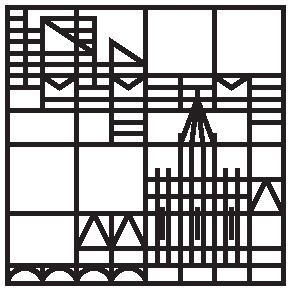
\includegraphics[width=5cm]{logo}
\\ \Large Universität Konstanz  \\ \vspace{4ex} \huge 
Skript zur Vorlesung\\ Höhere Quantentheorie und Elektrodynamik
\\ \vspace{4ex} \Large Prof. Dr. Wolfgang Belzig 
\\ Version vom 30. Juli 2012 \\ \vspace{4.5cm}
\normalsize Ursprünglichen Mitschrift von Birte Heinze im WS 09/10 \\ Ausführliche Überarbeitung von Tobias Lohse im WS 11/12 \vspace{-10cm}}
\author{}
\date{}
%\begin{document}

\subsection{Zeitabhängige Störungstheorie}
Näherungsmethoden stellen in der theoretischen Physik ein äußerst wichtiges Instrument dar, da nur die allerwenigsten und einfachsten Systeme direkt analytisch lösbar sind. Die Störungstheorie ist dabei das am häufigsten anwendbare Verfahren und beruht auf dem Grundgedanke den Hamiltonoperator eines Systems $\hat{\ham}$ durch den Hamiltonoperator $\hat{\ham}_0$ eines Systems anzunähern, dessen Lösung bereits bekannt ist und den Restterm, die {\bf Störung} $\hat{\ham}-\hat{\ham}_0=\lambda\hat{\ham}'$, in einer Potenzreihe zu entwickeln um deren Einfluss auf die Lösung anzunähern. Dieses Verfahren funktioniert immer dann gut, wenn der Einfluss der Störung $\lambda\hat{\ham}'$ auf das Gesamtsystem $\hat{\ham}=\hat{\ham}_0+\lambda\hat{\ham}'$ gering ist. In diesem Abschnitt soll insbesondere auf die Störungstheorie für einen zeitabhängigen Störterm $\hat{\ham}'(t)$ eingegangen werden. Dies ist beispielsweise relevant, wenn der Einfluss von Rauschen auf ein System untersucht werden soll. 

\subsubsection{Zeitabhängigkeit in der Schrödingertheorie}
Zunächst soll an dieser Stelle auf die Zeitabhängigkeit in der Schrödingertheorie eingegangen werden. Diese ergibt sich aus der Lösung der zeitabhängigen Schrödingergleichung (\ref{SG}): $\I\hbar\;\partial_t\ket{\psi(t)}=\hat{\ham}(\hat{\vec{p}},\hat{\vec{r}},t)\ket{\psi(t)}$. Im Normalfall hat der Hamiltonoperator dabei folgende Form: $\hat{\ham}(\hat{\vec{p}},\hat{\vec{r}},t) = T(\hat{\vec{p}}) + \hat{V}(\hat{\vec{r}},t)$. Im Falle eines zeitunabhängigen Potentials $\hat{V}(\hat{\vec{r}},t)=\hat{V}(\hat{\vec{r}})$ lässt sich die Zeitabhängigkeit wie bereits im ersten Abschnitt erwähnt in einen Phasenfaktor abseparieren $\ket{\psi(t)}=\exp(\I E t/\hbar)\ket{\psi}$. Die Schrödingergleichung wird dann zu einem zeitunabhängigen Eigenwertproblem (\ref{statSG}): $\hat{\ham}\ket{\psi}=E\ket{\psi}$. Deren Lösungen die Eigenzustände $\ket{\psi_n}$ mit den zugehörigen Eigenenergien $E_n$ sind. Die Allgemeine Lösung ergibt sich aus dem Superpositionsprinzip zu: 
\begin{eqnarray*}
	\ket{\psi(t)} = \sum_n c_n\cdot \e^{\frac{\I}{\hbar}E_n t}\ket{\psi_n}
\end{eqnarray*}
Die $c_n$ sind dabei komplexe Koeffizienten, die allein von den Anfangsbedingungen abhängen. 

Besitzt das Potential einen zeitabhängigen Teil $\hat{V}(\hat{\vec{r}},t)=\hat{V}_0(\hat{\vec{r}})+\hat{V}(\hat{\vec{r}},t)$, so kann der Hamiltonoperator in einen zeitunabhängigen und einen zeitabhängigen Teil aufgeteilt werden: $\hat{\ham}(\hat{\vec{p}},\hat{\vec{r}},t)=\hat{\ham}_0(\hat{\vec{p}},\hat{\vec{r}})+\hat{V}(\hat{\vec{r}},t)$. Da die Eigenzustände $\ket{\psi_n^{(0)}}$ des stationären Teils $\hat{\ham}_0$ eine vollständige Basis des Hilbertraums des Systems bilden, kann als Lösungsansatz folgendes verwendet werden: 
\begin{eqnarray*}
	\ket{\psi(t)} = \sum_n c_n(t)\cdot\ket{\psi_n^{(0)}}
\end{eqnarray*}
Die zeitabhängigen Koeffizienten $c_n(t)$ können nun durch einsetzten in die Schrödingergleichung gefunden werden. Dazu müssen $N$ Differenzialgleichungen erster Ordnung gelöst werden, deren Anfangsbedingungen bekannt sein sollten. $N$ ist dabei die Anzahl der Eigenzustände von $\hat{\ham}_0$.


\subsubsection{Zeitunabhängige Störungstheorie}
Wir wollen zunächst kurz auffrischen, wie im Falle einer zeitunabhängigen Störung die Störungstheorie funktioniert. Wir gehen also davon aus, dass sich der Hamiltonoperator $\hat{\ham}$ aufteilen lässt in einen Teil $\hat{\ham}_0$, dessen Lösung bekannt ist, und eine Störung $\lambda\hat{V}$. Der Parameter $\lambda$ hat hierbei keine besondere Bedeutung, es handelt sich lediglich um einen dimensionsloser Entwicklungsparameter. Wir schreiben den Hamiltonoperator also wie folgt: 
\begin{eqnarray*}
	\hat{\ham} = \hat{\ham}_0+\lambda \hat{V}
\end{eqnarray*}
Wir wollen nun die Eigenzustände $\ket{\psi_n}$ und Eigenenergien $E_n$ des gesamten Systems in einer Potenzreihe im Parameter $\lambda$  entwickeln: 
\begin{eqnarray*}
	E_n &=& E_n^{(0)} + \lambda E_n^{(1)} + \lambda^2 E_n^{(2)} + \ldots \;=\;  \sum_{k=0} \;\lambda^k E_n^{(k)}
	\\
	\ket{\psi_n} &=& \ket{\psi_n^{(0)}} + \lambda\ket{\psi_n^{(1)}} + \lambda^2 \ket{\psi_n^{(2)}} + \ldots \;=\; \sum_{k=0} \;\lambda^k \ket{\psi_n^{(k)}}
\end{eqnarray*}
Dabei sind die $\ket{\psi_n^{(0)}}$ und zugehörigen $E_n^{(0)}$ die bekannten Eigenzustände und Eigenenergien des ungestörten Hamiltonoperators. Die Eigenzustände des hermiteschen Operators $\hat{\ham}_0$ stellen eine vollständiges Orthonormalsystem $\braket{\psi_n^{(0)}}{\psi_m^{(0)}}=\delta_{n,m}$ dar und wir können die Normierung zweckmäßig auf $\braket{\psi_n^{(0)}}{\psi_n}=1$ festlegen. Falls die Eigenwerte nicht entartet sind, folgt unmittelbar, dass $\braket{\psi_n^{(0)}}{\psi_n^{(k)}}=\delta_{0,k}$ gilt. Wenn wir nun den Ansatz in die stationäre Schrödingergleichung (\ref{statSG}) einsetzen und nach Potenzen in $\lambda$ ordnen, so lassen sich durch Multiplikation der Gleichung mit $\bra{\psi_n^{(0)}}$ die Energien in den verschiedenen Ordnungen bestimmen als: 
\begin{eqnarray*}
	E_n^{(k)} &=& \bracket{\psi_n^{(0)}}{\lambda\hat{V}}{\psi_n^{(k-1)}}
\end{eqnarray*}
Um die Zustände $\ket{\psi_n^{(k)}}$ höherer Ordnung zu erhalten, multiplizieren wir die Gleichung mit $\bra{\psi_m^{(0)}}$ mit $m\neq n$. Für die Zustandskorrektur in erster Ordnung ergibt sich dann: 
\begin{eqnarray*}
	\ket{\psi_n^{(1)}} &=& \sum_{m\neq n} \; \frac{|\bracket{\psi_m^{(0)}}{\lambda\hat{V}}{\psi_n^{(0)}}|}{E_n^{(0)}-E_m^{(0)}}\cdot \ket{\psi_n^{(0)}}
\end{eqnarray*}
Im Falle einer Entartung des Eigensystems von $\hat{\ham}_0$ muss $\lambda\hat{V}$ zunächst im Unterraum der entarteten Zustände diagonalisiert werden, bevor die Störungstheorie angewandt werden kann. 


\subsubsection{Darstellung der Zeitabhängigkeiten in der Quantenmechanik}
Zeitabhängigkeiten können auf Grund der speziellen Struktur des Formalismus der Quantenmechanik auf verschiedene Art und Weise ausgedrückt werden. Man unterscheidet hauptsächlich drei Konventionen zur Zeitabhängigkeit von Zuständen und Observablen in der Quantenmechanik: 
\begin{itemize1}
	\item Das {\bf Schrödinger-Bild}, in dem wir bisher gearbeitet haben und in welchem die Zustände Zeitabhängig sind.  
	\item Das {\bf Heisenberg-Bild}, indem die Zeitabhängigkeit in die Observablen verschoben wird. 
	\item Das {\bf Dirac-Bild} oder {\bf Wechselwirkungsbild}, in welchem die Zeitentwicklung sowohl in den Observablen als auch in den Zuständen vorkommt. 
\end{itemize1}
Alle drei Konventionen können für die Lösung bestimmter Probleme vorteilhaft sein. Im allgemeinen sind die verschiedenen Bilder allerdings völlig gleichberechtigt. 

Im folgenden sollen die drei Bilder und ihre Unterschiede etwas genauer erläutert werden: 

\paragraph{Das Schrödinger-Bild}

Bisher haben wir uns ausschließlich mit dem Schrödinger-Bild befasst. In folgenden sollen dessen wichtigste Eigenschaften noch einmal zusammen gefasst werden:

\begin{itemize1}
	\item Die Zustandsvektoren sind zeitabhängig $\ket{\psi(t)}$. Die Zeitentwicklung der Zustandsvektoren wird durch die Schrödingergleichung beschrieben: $\I\hbar\;\dell_t\ket{\psi(t)} = \hat{\ham}(t) \ket{\psi(t)}$
	\item Operatoren $\hat{A}(t)$ können explizit von der Zeit abhängen, sind aber keiner Zeitentwicklung unterworfen. 
	\item Der Erwartungswert eines Operators ist das gemittelte Messergebnisse der Observablen und berechnet sich damit als $\EW{\hat{A}(t)} = \bracket{\psi(t)}{\hat{A}(t)}{\psi(t)}$. 
	\item Für zeitunabhängigen Hamiltonoperatoren $\hat{\ham(t)}=\hat{\ham}_0$ ist eine formale Lösung der Schrödingergleichung gegeben durch: 
	\begin{eqnarray*}
		\ket{\psi(t)} &=& \underbrace{\e^{-\frac{\I}{\hbar}\cdot\hat{\ham}_0\;t}}_{=\hat{U}_0} \ket{\psi(0)} = \hat{U}_0\ket{\psi(0)}
	\end{eqnarray*}
	Der Operator $\hat{U}_0=\exp(-\I/\hbar\cdot\hat{\ham}_0\;t)$ wird dabei als unitärer {\bf Zeitentwicklungsoperator} des zeitunabhängigen Hamiltonoperators $\hat{\ham}_0$ bezeichnet. Unitäre Operatoren erfüllen die Gleichung $\hat{U}^{\dagger}\hat{U}=\hat{U}\hat{U}^{\dagger}=1$. 
\end{itemize1}

\paragraph{Das Heisenberg-Bild}

Im Heisenberg-Bild wird die Zeitabhängigkeit in die Operatoren verschoben. Operatoren und Zustände im Heisenberg-Bild werden häufig mit einem Index $_H$ versehen um sie als solche zu kennzeichnen. Der Formalismus ist durch folgende Definitionen und Eigenschaften gekennzeichnet: 

\begin{itemize1}
	\item Der Zustandsvektor im Heisenberg-Bild ist definiert als: 
	\begin{eqnarray*}
		\ket{\psi_H} &=& \hat{U}^{\dagger}\ket{\psi(t)} \quad=\quad \ket{\psi(0)}
	\end{eqnarray*}
	Damit sind die Zustandsvektoren zeitunabhängig und die Zeitentwicklung kann nicht mehr durch die Schrödingergleichung beschrieben werden. 
	\item Der unitäre Zeitentwicklungsoperator $\hat{U}$ ist dabei im einfachsten Fall eines zeitunabhängigen Hamilton Operators $\hat{\ham}_0$ gegeben durch $\hat{U}_0(t)=\exp(-\I/\hbar\cdot\hat{\ham}_0\;t)$, im Falle eines zeitabhängigen Hamilton Operators kann er ebenfalls definiert werden, seine Darstellung wird allerdings komplizierter. Die definierende Bestimmung für den Zeitentwicklungsoperator ist die Differentialgleichung $\I\hbar \dell_t \hat{U}(t)=\hat{\ham}(t)\hat{U}(t)$. Mehr zu deren allgemeiner Lösung im übernächsten Paragraph. 
	\item Die Operatoren im Heisenberg-Bild sind definiert als: 
	\begin{eqnarray*}
		\hat{A}_H(t) &=& \hat{U}^{\dagger}\;\hat{A}(t)\;\hat{U}
	\end{eqnarray*}
	\item Der Erwartungswert muss in allen Bildern gleich bleiben. Dies lässt sich leicht zeigen: $\EW{\hat{A}}=\bracket{\psi(t)}{\hat{A(t)}}{\psi(t)}=\bracket{\psi(0)}{\hat{U}^{\dagger}\hat{A}(t)\hat{U}}{\psi(0)}=\bracket{\psi_H}{\hat{A}_H(t)}{\psi_H}$. 
	\item Die Zeitentwicklung ist im Heisenberg-Bild durch eine Operator-Gleichung bestimmt, welche sich aus der Definition des Zeitentwicklungsoperators ergibt als: 
	\begin{eqnarray}
		\frac{\mathrm{d}}{\mathrm{d}t} \hat{A}_H(t) &=& \frac{\mathrm{d}}{\mathrm{d}t} \Big(\hat{U}^{\dagger}(t)\hat{A}(t)\hat{U}(t)\Big) = \hat{U}^{\dagger}\Big(\underbrace{\frac{\I}{\hbar}\hat{\ham}\hat{A}(t)-\frac{\I}{\hbar}\hat{A}(t)\hat{\ham}}_{=\I/\hbar\cdot[\hat{\ham},\hat{A}(t)]}+\dell_tA(t)\Big)\hat{U} \nonumber
		\\
		&=& \frac{\I}{\hbar}\cdot[\hat{H},\hat{A}_H(t)]+\big(\dell_tA(t)\big)_H \label{HG}
	\end{eqnarray}
	Diese Gleichung wird auch als {\bf Heisenberg Gleichung} bezeichnet. Man beachte außerdem, dass selbstverständlich $[\hat{H},\hat{A}_H(t)]=\big([\hat{H},\hat{A}(t)]\big)_H$ gilt, da der Hamiltonoperator mit dem Zeitentwicklungsoperator vertauscht. 
\end{itemize1} 


\paragraph{Das Wechselwirkungsbild}

Für Probleme mit zeitabhängigem Hamiltonoperator $\hat{\ham}(t)=\hat{\ham}_0+\hat{V}(t)$ eignet sich die Einführung eines gemischten Bildes, in dem sowohl Zustände als auch Operatoren teilweise zeitabhängig sind. Dieses Bild wird als Wechselwirkungsbild oder Dirac-Bild bezeichnet und die Zustände und Operatoren werden häufig mit einem Index $_I$ für englisch 'interaction' gekennzeichnet. Folgendes sind die essentiellen Definitionen: 

\begin{itemize1}
	\item Das Wechselwirkungsbild ist in einem System mit einem zeitabhängigen Hamiltonoperator $\hat{\ham}(t)$ definiert, welcher aus einem zeitunabhängigen Teil $\hat{\ham}_0$ und einem zeitabhängigen Teil $\hat{V}(t)$ zusammengesetzt ist: 
	\begin{eqnarray*}
		\hat{\ham}(t) &=& \hat{\ham}_0+\hat{V}(t) 
	\end{eqnarray*}
	Für den zeitunabhängigen Teil des Hamiltonoperators wird der Zeitentwicklungsoperator $\hat{U}_0=\exp(-\I/\hbar\cdot \hat{\ham}_0t)$ definiert. 
	\item Die Zustände im Wechselwirkungsbild sind wie folgt definiert: 
	\begin{eqnarray*}
		\ket{\psi_I(t)} &=& \hat{U}_0^{\dagger}\ket{\psi(t)} \;=\; \e^{\;\frac{\I}{\hbar}\; \hat{\ham}_0\; t}\ket{\psi(t)}
	\end{eqnarray*}
	\item Die Operatoren im Wechselwirkungsbild sind definiert als: 
	\begin{eqnarray*}
		\hat{A}_I(t) &=& \hat{U}^{\dagger}_0\;\hat{A}(t)\;\hat{U}_0
	\end{eqnarray*}
	\item Die Bewegungsgleichung im Wechselwirkungsbild ergibt sich aus der Schrödingergleichung: 
	\begin{eqnarray}
		\I\hbar\;\dell_t \ket{\psi_I(t)} &=& \I\hbar\;\dell_t \;\Big(\hat{U}^{\dagger}_0(t) \ket{\psi(t)}\Big) = \hat{U}^{\dagger}_0 \big(\I\hbar\;\dell_t-\hat{\ham}_0\big)\ket{\psi(t)} = \hat{U}^{\dagger}_0\big(\underbrace{\hat{\ham}-\hat{\ham}_0}_{=\hat{V}(t)}\big)\underbrace{\hat{U}_0 \hat{U}^{\dagger}_0}_{=\1} \ket{\psi(t)} \nonumber
		\\
		&=& \hat{V}_I(t) \ket{\psi_I(t)} \label{WechselwirkungsbildSG}
	\end{eqnarray}
	Die Zeitentwicklung in Wechselwirkungsbild ist also allein durch $\hat{V}_I$ bestimmt. 
\end{itemize1}

\subsubsection{Allgemeine Lösung der Schrödingergleichung im Wechselwirkungs}

Wir wollen nun die Schrödingerlgeichung des Wechselwirkungsbilds (\ref{WechselwirkungsbildSG}) ganz allgemein lösen. Dazu verwenden wir die Anfangsbedingungen $\ket{\psi_I(0)}=\ket{\psi(0)}=:\ket{\psi_0}$ und integrieren Schrödingerlgeichung des Wechselwirkungsbilds (\ref{WechselwirkungsbildSG}): 
\begin{eqnarray*}
	\ket{\psi_I(t)} &=& \ket{\psi_0} - \frac{\I}{\hbar}\int_0^t \mathrm{d}t'\; \hat{V}_I(t') \ket{\psi_I(t')} 
\end{eqnarray*}
Wenn wir nun die linke Seite in die Rechte einsetzen erhalten wir folgende Gleichung: 
\begin{eqnarray*}
	\ket{\psi_I(t)} &=& \ket{\psi_0} - \frac{\I}{\hbar}\int_0^t\mathrm{d}t'\; \hat{V}_I(t') \ket{\psi_0} + \Big(\frac{-\I}{\hbar}\Big)^2 \int_0^t \mathrm{d}t'\; \int_0^{t'}\mathrm{d}t''\; \hat{V}_I(t')\hat{V}_I(t'')\ket{\psi_I(t'')}
\end{eqnarray*}
Durch wiederholtes Einsetzten der linken Seite in die rechte, entsteht eine unendliche Summe und die Gleichung erhält folgende Form:
\begin{eqnarray*}
	\ket{\psi_I(t)} &=& \underbrace{\sum_{n=0}^{\infty} \Big(\frac{-\I}{\hbar}\Big)^n \int_0^t\mathrm{d}t_1 \int_0^{t_1}\mathrm{d}t_2\;\; \cdots \int_0^{t_{n-1}}\mathrm{d}t_n\; \hat{V}_I(t_1)\hat{V}_I(t_2) \cdots \hat{V}_I(t_n)}_{=:\;\hat{U}_I(t,0)} \ket{\psi_0}
\end{eqnarray*}
Damit haben wir einen Zeitentwicklungsoperator $\hat{U}_I(t,0)$ für das Potential $\hat{V}_I(t)$ definiert. Dabei ist auf die Zeitordnung zu achten, da die Operatoren $\hat{V}_I(t_i)$ zu verschiedenen Zeiten $t_i$ nicht notwendigerweise vertauschen. Der Operator mit dem kleinsten Zeitparameter steht am weitesten rechts: $t\geq t_1\geq t_2\geq \cdots \geq t_n\geq 0$. Um diesem Umstand Rechnung zu tragen führen wir daher den Dysonschen {\bf Zeitordnungsoperator} $\widehat{T}$ ein, welcher zwei Operatoren vertauscht, auch wenn deren Kommutator nicht null ist:
\begin{eqnarray*}
	\widehat{T}\big(\hat{A}(t)\hat{B}(t')\big) = \left\{ \begin{array}{rl} \hat{A}(t)\hat{B}(t') & t > t'\\\hat{B}(t')\hat{A}(t) & t < t'\end{array}\right. 
\end{eqnarray*}
Mit Hilfe des Zeitordnungsoperators lässt sich nun die Gleichung wie folgt umformen:
\begin{eqnarray*}
	&&\!\!\!\!\! \widehat{T}\;\bigg( \int_0^{t}\mathrm{d}t_1 \int_0^{t_1}\mathrm{d}t_2\;\cdots\int_0^{t_{n-1}}\mathrm{d}t_n\; \hat{V}_I(t_1)\hat{V}_I(t_2) \cdots \hat{V}_I(t_n) \bigg)
	\\
	&&\!=\;\widehat{T}\;\bigg( \frac{1}{n!}\cdot \int_0^{t}\mathrm{d}t_1 \int_0^{t}\mathrm{d}t_2\;\cdots\int_0^{t}\mathrm{d}t_n\; \hat{V}_I(t_1)\hat{V}_I(t_2) \cdots \hat{V}_I(t_n) \bigg) \;=\; \widehat{T}\;\Bigg( \frac{1}{n!}\cdot \bigg(\int_0^{t}\mathrm{d}t'\; \hat{V}_I(t')\bigg)^n \Bigg)
\end{eqnarray*}
Die Korrektheit des Faktors $1/n!$, welcher bei der Erweiterung der Integrale auftaucht, lässt sich beweisen, indem die Gleichung nach $t$ abgeleitet wird. Der Zeitentwicklungsoperator $\hat{U}_I(t,0)$ lässt sich damit nun sehr kompakt schreiben als: 
\begin{eqnarray}
	\hat{U}_I(t,0) &=& \widehat{T}\;\Bigg( \sum_{n=0}^{\infty} \cdot \frac{1}{n!}\cdot \bigg(\!\!-\frac{\I}{\hbar}\cdot\int_0^{t}\mathrm{d}t'\; \hat{V}_I(t')\bigg)^n \Bigg) \;=\;\; \widehat{T}\;\exp \bigg(\!\!-\frac{\I}{\hbar}\cdot\int_0^{t}\mathrm{d}t'\; \hat{V}_I(t')\bigg) \qquad\label{Zeitentwicklungsoperator}
\end{eqnarray}
Somit haben wir eine allgemeine Form des Zeitentwicklungsoperators hergeleitet. Im folgenden sollen dessen Eigenschaften zusammen gefasst werden: 

\begin{itemize1}
	\item Der Zeitentwicklungsoperator stellt die Lösung der folgenden Differentialgleichung dar, welche sich direkt aus der Schrödingergleichung ableitet:
	\begin{eqnarray*}
		\I\hbar\;\dell_t\;\hat{U}_I(t,0) = \hat{U}_I(t,0)\;\hat{V}_I(t)
	\end{eqnarray*}
	Da bei der Lösung dieser Differentialgleichung keine Annahmen über die Form von $\hat{V}_I$ getroffen wurden, stellt die Definition in Gleichung (\ref{Zeitentwicklungsoperator}) die allgemeine Definition eines Zeitentwicklungsoperators $\hat{U}$ eines Quantenmechanischen Systems mit einem beliebigen Hamiltonoperator $\hat{\ham}(t)=\hat{V}_I(t)$ dar, welcher beispielsweise für die Formulierung des Heisenberg-Bilds genutzt werden kann. 
	\item Für zeitunabhängige Hamiltonoperatoren $\hat{V}_I(t)=\hat{\ham}$ ergibt sich sofort der bereits bekannte Zeitentwicklungsoperator: $\hat{U}_0=\widehat{T}\exp(-\I/\hbar\cdot\int_0^t\mathrm{d}t'\;\hat{\ham}_0) = \exp(-\I/\hbar\cdot \hat{\ham}_0\;t)$. 
	\item Es gilt wie man leicht sieht $\hat{U}_I(t,t) = \1$. 
	\item Der Zeitentwicklungsoperator zwischen zwei Zeitpunkten $t$ und $t'$ kann wie man leicht sieht immer auf folgende weise zusammengesetzt werden: $\hat{U}_I(t,t')=\hat{U}_I(t,t'') \hat{U}_I(t'',t')$:
	\item Falls für alle $t,t'$ gilt $[\hat{V}_I(t),\hat{V}_I(t')]=0$, so wird der Zeitordnungsoperator $\widehat{T}$ in Gleichung (\ref{Zeitentwicklungsoperator}) überflüssig.
	\item Da der Zeitentwicklungsoperator durch eine Potenzreihe gegeben ist, kann sich die Zeitentwicklung nähern lassen, wenn wir die Potenzreihe ab einer bestimmten Ordnung abbrechen lassen. 
	\item In der niedrigsten Ordnung ist der Zeitordnungsoperator $\widehat{T}$ ebenfalls überflüssig und der Zeitenetwicklungsoperator ergibt sich zu: $\hat{U}_I(t,0) = \1-\I/\hbar\cdot\int_0^t\mathrm{d}t'\; \hat{V}_I(t')$
	\item Es lässt sich außerdem zeigen, dass folgendes gilt: $\hat{U}_I(t,0)-\1 = \hat{U}_I^{\dagger}(t,0) = \hat{U}_I(0,t)$. 
\end{itemize1}


\subsubsection{Übergangswahrscheinlichkeiten}

Anstatt die gesamte Zeitentwicklung eines Systems zu berechnen ist es häufig interessant einfach nur die Übergangswahrscheinlichkeit von einem Zustand in einen anderen zu berechnen, wenn das System gestört wird. 

Dies wollen wir im folgenden Abschnitt für ein System mit zeitunabhängigem Hamiltonoperaotr $\hat{\ham}_0$ und eine zeitabhängige Störung $\hat{V}(t)$ tun, welche zum Zeitpunkt $t=0$ eingeschaltet wird: $\hat{V}(t<0)=0$. Eine solch Störung könnte beispielsweise ein für eine gewisse Zeitspanne eingeschaltetes äußeres Feld oder der Vorbeiflug eines geladenen Teilchens sein. Das System befindet sich also zum Zeitpunkt $t=0$ in einem Initialzustand $\ket{i}$. Die Übergangswahrscheinlichkeit $P_{i\to f}(t)$ in einem Finalzustand $\ket{f}$ zum Zeitpunkt $t$ ist dann gegeben durch: 
\begin{eqnarray*}
	P_{i\to f}(t) &=& \big|\braket{f}{\psi(t)}\big|^2 = \big|\bracket{f}{\hat{U}_0}{\psi_I(t)} = \big|\bracket{f}{\e^{-\frac{\I}{\hbar}\cdot \hat{\ham}_0\;t}}{\psi_I(t)}\big|^2
\end{eqnarray*}
Wobei $\ket{\psi(t)}$ der Zustand des Systems zum Zeitpunkt $t$ ist. Wenn der Finalzustand $\ket{f}$ nun ein Eigenzustand des zeitunabhängigen Hamiltonoperators mit Eigenenergie $E_f$ ist, so verursacht $\hat{U}_0$ nur eine Phasenverschiebung, welche den Betrag nicht ändert: 
\begin{eqnarray*}
	P_{i\rightarrow f}(t)=\big|\bracket{f}{\e^{-\frac{\I}{\hbar}\cdot \hat{\ham}_0\;t}}{\psi_I(t)}\big|^2 = \big|\e^{-\frac{\I}{\hbar}\cdot E_f\;t}\cdot\braket{f}{\psi_I(t)}\big|^2 &=& \big|\braket{f}{\psi_I(t)}\big|^2 = \big|\bracket{f}{\hat{U}_I}{i}\big|^2 
\end{eqnarray*}
Für den Fall, dass $\ket{i}$ und $\ket{f}$ orthogonal zueinander sind: $\braket{i}{f}=0$ und auch $\ket{i}$ ein Eigenzustand von $\hat{\ham}_0$ mit Eigenenergie $E_i$ ist ergibt sich dann in Näherung erster Ordnung für $\hat{U}_I$, also für relativ kleine Störpotentiale und relativ kleine Zeitintervalle $t$ die Übergangswahrscheinlichkeit zu: 
\begin{eqnarray}
	P_{i\to f}(t) &\approx& \Big|\braket{f}{i} - \frac{\I}{\hbar} \int_0^t\mathrm{d}t'\; \bracket{f}{\hat{V}_I(t')}{i} \Big|^2 = \frac{1}{\hbar^2}\cdot \Big|\int_0^t\mathrm{d}t'\; \bracket{f}{\hat{U}^{\dagger}_0(t')\;\hat{V}(t')\;\hat{U}_0(t')}{i} \Big|^2 \nonumber
	\\
	&& \qquad\qquad= \frac{1}{\hbar^2}\cdot \Big|\int_0^t\mathrm{d}t'\; \exp\Big(\I\cdot\underbrace{\frac{E_f-E_i}{\hbar}}_{=:\;\omega_{fi}}\cdot t'\Big) \cdot\bracket{f}{\hat{V}(t')}{i} \Big|^2 \nonumber
	\\
	\Rightarrow\quad P_{i\to f}(t) &\approx& \frac{1}{\hbar^2}\cdot \Big|\int_0^t\mathrm{d}t'\; \e^{\;\I\;\omega_{fi}\cdot t'} \cdot\bracket{f}{\hat{V}(t')}{i}\;\Big|^2 \label{Uebergangswahrscheinlichkeit} 
\end{eqnarray} 
Wir haben somit eine recht einfache Näherung für die Übergangswahrscheinlichkeit zwischen zwei orthogonalen Eigenzuständen $\ket{i}$ und $\ket{f}$ des zeitunabhängigen Hamiltonoperators unter Einfluss einer zeitlichen Störung $\hat{V}(t)$ gefunden. Die Näherung funktioniert nicht, falls $P_{i\rightarrow f}(t)\approx0$ gilt. 


\paragraph{Konstante Störung}

Übergangswahrscheinlichkeit im Falle eines nach dem Einschalten zeitlich konstanten Potentials untersuchen. Mit Hilfe der Theta-Funktion $\Theta(t>0)=1\land\Theta(t<0)=0$, lässt sich dieses schreiben als: $\hat{V}(t)=\Theta(t)\cdot\hat{V}$. Gleichung (\ref{Uebergangswahrscheinlichkeit}) lässt sich in diesem Fall vereinfachen zu:  
\begin{eqnarray*}
	P_{i\to f}(t,\omega_{fi}) = \underbrace{\frac{1}{\hbar^2}\cdot\big|\bracket{f}{\hat{V}}{i}\big|^2 }_{=:\;M_{fi}} \cdot 
	\Big|\int_0^t\mathrm{d}t'\; \e^{\;\I\;\omega_{fi}\cdot t'} \Big|^2 = M_{fi} \cdot \Big| \frac{\e^{\;\I\;\omega_{fi}\cdot t'}-1}{\I\;\omega_{fi}}\Big|^2 =\; M_{fi} \cdot\frac{\sin^2\big(\frac{\omega_{fi}}{2}\cdot t\big)}{\big(\frac{\omega_{fi}}{2}\big)^2}
\end{eqnarray*}
Die Übergangswahrscheinlichkeit hängt also linear vom Matrixelement $M_{fi}$ ab und wird maximal für kleine $\omega_{fi}$, also für Zustände mit nur wenig unterschiedlichen Energieeigenwerten. Die Übergangswahrscheinlichkeit wird null für $\omega_{fi}=2\pi/t\cdot n$ mit $n\in\mathbb{N}$ und wird für große $\omega_{fi}$ sehr schnell klein, die Halbwertsbreite ist proportional zu $1/t$. Das Maximum von $P_{i\to f}(t,\omega_{fi})$ ergibt sich für $\omega_{fi}\to0$ mit l'Hospitale zu: 
\begin{eqnarray*}
	\max\big(P_{i\to f}(t)\big) &=& \lim_{\omega_{fi}\to0}M_{fi}\cdot\frac{\sin^2\big(\frac{\omega_{fi}}{2}\cdot t\big)}{\big(\frac{\omega_{fi}}{2}\big)^2}= M_{fi}\cdot t^2 = \frac{1}{\hbar^2}\cdot\big|\bracket{f}{\hat{V}}{i}\big|^2 \cdot t^2
\end{eqnarray*}
Der folgende Plot soll das Verhalten von $P_{i\to f}(t,\omega_{fi})$ noch einmal veranschaulichend darstellen:
\vspace{-2ex}\begin{figure}[!h]\center
	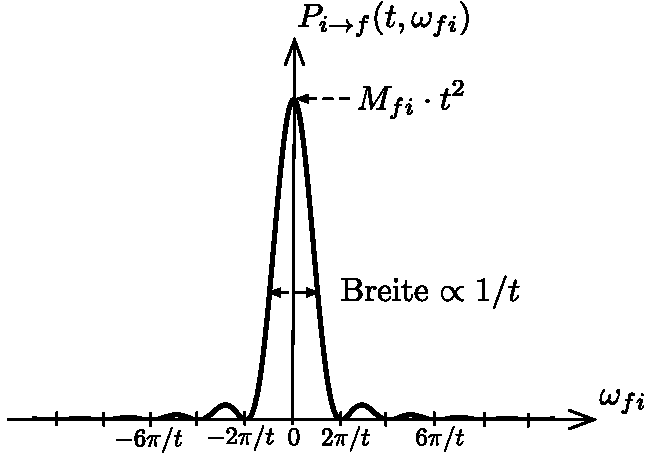
\includegraphics[scale=.75]{Figs/Sin2Plot}
\end{figure}\vspace{-4ex}

Interessant ist der Grenzfall für lange Zeiten $t\to\infty$. Für diesen können wir, wenn wir $\omega_{fi}:=\alpha$ substituieren, die folgende Funktionenfolge $\delta_t(\alpha)$ definieren: 
\begin{eqnarray*}
	P_{i\to f}(t,\omega_{fi}) = M_{fi}\cdot\pi\cdot t\cdot \frac{\sin^2\big(\frac{\omega_{fi}}{2}\cdot t\big)}{\pi \big(\frac{\omega_{fi}}{2}\big)^2\cdot t} = M_{fi}\cdot\pi\cdot t\cdot\underbrace{\frac{\sin^2(\alpha\cdot t)}{\pi\alpha^2\cdot t}}_{=:\;\delta_t(\alpha)} = M_{fi}\cdot\pi\cdot t\cdot \delta_t(\alpha)
\end{eqnarray*}
Die Funktionenfolge $\delta_t(\alpha)$ hat in einem Kontinuum folgende Eigenschaft: 
\begin{eqnarray*}
	\lim_{t\to\infty}\int_{-\infty}^{\infty}\mathrm{d}\alpha\;\delta_t(\alpha)\cdot F(\alpha) = \lim_{t\to\infty}\frac{1}{\pi}\underbrace{\int_{-\infty}^{\infty}\mathrm{d}y\;\frac{\sin^2y}{y^2}}_{=\;\pi}\cdot F(y/t) = F(0)
\end{eqnarray*}
Für $t\to\infty$ ist $\delta_t(\alpha)$ also eine Darstellung der Deltafunktion. Damit ergibt sich dann die Übergangswahrscheinlichkeit, wenn $\omega_{fi}$ als Kontinuum betrachtet werden kann zu: 
\begin{eqnarray*}
	\lim_{t\to\infty}P_{i\to f}(t) &=& M_{fi}\cdot\pi\cdot t\cdot \delta\Big(\frac{E_f-E_i}{2\hbar}\Big) = 2\pi\hbar\cdot M_{fi}\cdot t\cdot \delta(E_f-E_i)
\end{eqnarray*}
Für eine lange andauernde relativ kleine Störung in einem kontinuierlichen Energiespektrum haben wir somit eine einfache Darstellung für die {\bf Übergangsrate} $\Gamma_{i\to f}=\dell_t\;P_{i\to f}$ gefunden, welche in zahlreichen physikalischen Problemen sehr nützlich ist und auch als {\bf Fermis Goldene Regel} bezeichnet wird: 
\begin{eqnarray}
	\Gamma_{i\to f} =  \frac{2\pi}{\hbar}\cdot\big|\bracket{f}{\hat{V}}{i}\big|^2 \cdot \delta(E_f-E_i) \label{FermisGoldeneRegel}
\end{eqnarray}
Dabei mag es vielleicht zunächst etwas verwirrend erscheinen, dass wir für die Herleitung von (\ref{Uebergangswahrscheinlichkeit}) in erster Ordnung der zeitabhängigen Störungstheorie angenommen haben, dass das Zeitintervall $t$ relativ klein ist und nun eine Näherung für $t\to\infty$ gemacht haben, was in einer mit der Zeit unbegrenzt linear anwachsenden Überganswahrscheinlichkeit resultiert ist. Dies ist natürlich nur zulässig sofern die Störung innerhalb des Zeitintervalls $t$ klein bleibt: $|\bracket{i}{\hat{V}}{f}|^2\cdot t\ll1$. Die Näherung durch die Deltafunktion wird legitim, wenn die Breite der Funktion $P_{i\to f}(E_f-E_i)$, welche wir auf halbem Weg zum ersten Minimum als $2\pi\hbar/t$ abschätzen können (Man beachte $E_f-E_i=2\cdot\hbar\omega_{fi}$), deutlich kleiner ist als die Breite der kontinuierlichen Energieverteilung $\Delta\varepsilon$. Andererseits muss die Anzahl der Zustände innerhalb des Peaks von $P_{i\to f}(E_f-E_i)$ groß genug sein, um die Energie als Kontinuum zu nähern, das heißt der Abstand zwischen den einzelnen Energien $\delta\varepsilon$ muss viel kleiner als $2\pi\hbar/t$ sein. Im folgenden Plot ist die Funktion $P_{i\to f}(E_f-E_i)$ in der Energieverteilung mit Breite $\Delta\varepsilon$ mit den einzelnen Energien im Abstand $\delta\varepsilon$ noch einmal schematisch dargestellt: 
\vspace{-2ex}\begin{figure}[!h]\center
	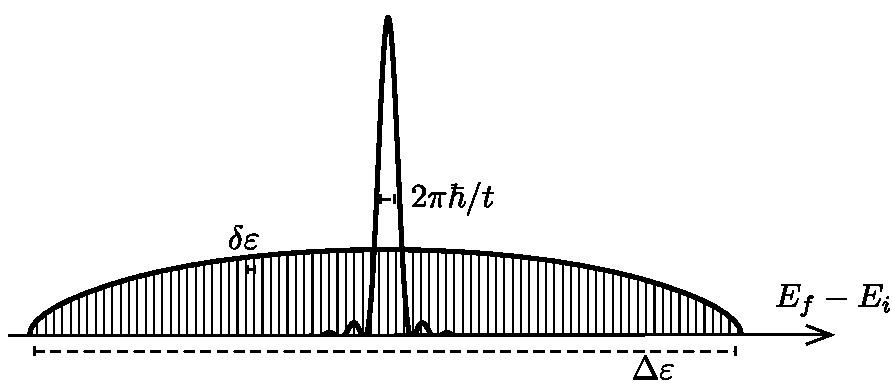
\includegraphics[scale=.75]{Figs/Escale}
\end{figure}\vspace{-4ex} 

Die Bedingung für den Zeitmaßstab in der Kontinuums und Deltapeak Näherung lautet also zusammengefasst wie folgt: 
\begin{eqnarray*}
	\frac{2 \pi \hbar}{\delta\varepsilon} \quad\gg\quad t \quad\gg\quad \frac{2\pi \hbar}{\Delta\varepsilon}
\end{eqnarray*}
Es mag außerdem etwas seltsam erscheinen, dass die Übergangswahrscheinlichkeit durch eine Deltafunktion beschrieben wird. Die Formel macht mehr Sinn, wenn wir statt der Übergangswahrscheinlichkeit in den Zustand eines Energieeigenwerts den Übergang in ein Energieintervall betrachten, was auf Grund von Messungenauigkeiten in allen realen Prozessen natürlich der Fall ist. 

Um die Übergangsrate in ein Intervall von Zuständen zu beschreiben, müssen wir zunächst die {\bf Zustandsdichte} $\varrho(\varepsilon)$ definieren, welche in jeglichen Viel-Teilchen Theorien eine wichtige Rolle spielt. Diese ist definiert durch die Aussage, dass $\varrho(\varepsilon)\mathrm{d}\varepsilon$ die Zahl der ungestörten Eigenzustände mit Energiewerten im Intervall $\varepsilon+\mathrm{d}\varepsilon$ angibt. Dies bedeutet wir können in der Kontinuumsnäherung $\delta\varepsilon\ll2\pi\hbar/t$ folgendes schreiben: $\varrho(\varepsilon)=\sum_f\delta(\varepsilon - E_f)$. Und für eine beliebige Funktion $F(E)$ lässt sich die Summe über mehrere Energien schreiben als $\sum_f F(E_f) = \int\mathrm{d}\varepsilon\;\varrho(\varepsilon)F(\varepsilon)$. Damit ergibt sich die Übergangsrate von $\ket{i}$ in ein Intervall von Endzuständen $\Delta\varepsilon_f$ zu: 
\begin{eqnarray*}
	\Gamma_{i\to\Delta\varepsilon_f} &=& \sum_{f\in\Delta\varepsilon_f} \Gamma_{i\to f}(\varepsilon_f) = \int_{\Delta\varepsilon_f}\mathrm{d}\varepsilon_f\;\varrho(\varepsilon_f)\cdot\Gamma_{i\to f}(\varepsilon_f)
\end{eqnarray*}
Im Falle eines breiten Energiespektrums $\Delta\varepsilon_f\gg2\pi\hbar/t$ können wir $\Gamma_{i\to f}(\varepsilon_f)$ durch die Deltafunktion nähern und dürfen das Integral von $-\infty$ bis $\infty$ laufen lassen. Außerdem können wir davon ausgehen, dass wir das Matrixelement an der Stelle $E_f=E_i$ als konstante vor das Integral ziehen können. Damit ergibt sich dann folgende Übergangsrate für Übergänge mit Energieerhaltung: 
\begin{eqnarray*}
	\Gamma_i &=& \frac{2\pi}{\hbar}\cdot\big|\bracket{f}{\hat{V}}{i}\big|^2 \cdot\varrho(E_i)
\end{eqnarray*}
Die Goldene Regel kann beispielsweise angewandt werden, wenn wir die Streuung eines Teilchens betrachten, durch die sich dessen Impuls ändert, oder den $\alpha$-Zerfall, indem die Teilchen mit einem bestimmten Impuls aus dem Kernpotential entkommen oder auch für optische Übergänge, bei denen Photonen emittiert werden. 


\paragraph{Periodische Störung}

Wir wollen nun die Goldene Regel noch auf den Fall eines nach dem einschalten periodisch variierenden Potentials erweitern, beispielsweise ein oszillierendes elektromagnetisches Feld. Wir nehmen an, dass das Potential die folgende Form hat: 
\begin{eqnarray*}
	\hat{V}(t) = \Theta(t)\big(\hat{F}^+ \cdot \e^{\;\I\omega t} + \hat{F}^- \cdot \e^{-\I\omega t}\big)
\end{eqnarray*}
Aus Gleichung (\ref{Uebergangswahrscheinlichkeit}) ergibt sich dann folgende Form für die Übergangswahrscheinlichkeit in erster Ordnung zeitabhängiger Störungstheorie: 
\begin{eqnarray*}
	P_{i\rightarrow f} (t) = \frac{1}{\hbar} \Big| \int_0^t \mathrm{d}t' \big(\e^{\;\I(\omega_{fi}-\omega)t'}\cdot\bracket{f}{\hat{F}^-}{i} + \e^{\;\I(\omega_{fi}+\omega)t'}\cdot\bracket{f}{\hat{F}^+}{i} \big) \Big|^2
\end{eqnarray*}
Für einigermaßen große Zeiten $2\pi/t\gg\omega$ ist der Überlapp zwischen den beiden $\delta$-artigen Funktionen quasi nicht vorhanden und die gemischten Terme im Absolutbetragsquadrat haben keinen Beitrag. Wir erhalten somit eine Superposition zweier Funktionen $\delta_t(\omega_{fi}\pm\omega)$, deren Maxima bei $\omega$ und $-\omega$ liegen. Der Verlauf der Übergangswahrscheinlichkeit für diesen Fall ist in dem folgenden Diagramm schematisch dargestellt:\newpage 
\begin{figure}[!h] \centering
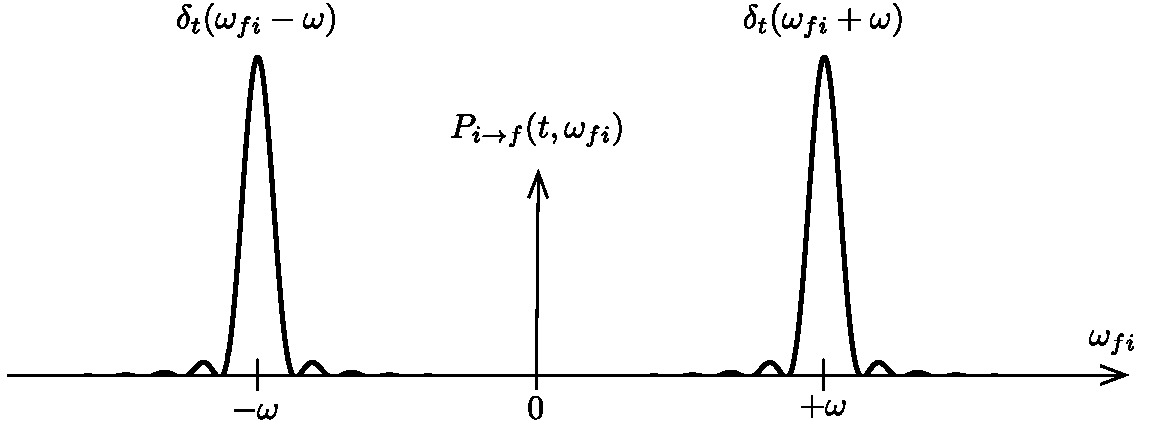
\includegraphics[scale=0.75]{Figs/DoppelSinPlot}
\end{figure}\vspace{-2ex}

Die Goldene Regel für die Übergangsrate im periodischen Fall lässt sich somit schreiben als: 
\begin{eqnarray*}
	\Gamma_{i\rightarrow f} &=& \frac{2\pi}{\hbar} \Big( \big|\bracket{f}{\hat{F}^-}{i}\big|^2\cdot \delta(E_f-E_i-\hbar \omega) + \big|\bracket{f}{\hat{F}^+}{i}\big|^2\cdot \delta(E_f-E_i +\hbar \omega) \Big)
\end{eqnarray*}
Damit gibt es nur Übergänge zwischen Anfangs- und Endzuständen, welche sich um die Energie $\hbar\omega$ unterscheiden. Die Energieerhaltung wird unter Absorption der Endzustandsenergiedifferenz erhalten. Bei Absorption gilt $E_f=E_i+\hbar\omega$ und bei Emission: $E_f=E_i-\hbar\omega$. 

Die Quantenfeldtheorie fordert an dieser Stelle einen Korrekturterm, der im letzten Kapitel behandelt werden wird.

%\end{document} \newpage 
\thispagestyle{plain} %\documentclass[a4paper,12pt,final,twoside]{scrartcl}
\setcounter{secnumdepth}{3}
\setcounter{tocdepth}{5}

\usepackage[utf8]{inputenc}
\usepackage[T1]{fontenc}
\linespread{1.4}
\usepackage{dsfont}
\usepackage{amsfonts}
\usepackage{amsmath}
\usepackage{amssymb}
\usepackage{amsthm}
\usepackage{mathtools}
\usepackage{mathbbol}
\usepackage{amsmath1}
\usepackage[ngerman]{babel}
\usepackage{bibgerm}
\usepackage[pdftex]{graphicx}
%\usepackage{mathpazo}
\usepackage{floatflt}
%%\usepackage{epsfig}
\usepackage{wrapfig}
\usepackage{graphicx}
\usepackage{tabularx}
\usepackage{caption} 
\usepackage{multicol} 
\usepackage{mathrsfs}
%\usepackage{pspicture}
%\usepackage{eepic}
%\usepackage{epic}
%\usepackage{trfsigns}

%\usepackage[ansinew]{inputenc}
\usepackage{longtable,array,dcolumn}
%\usepackage{ngerman}
\usepackage{epic}
\usepackage{rotate}
\usepackage{graphpap}
\usepackage{amssymb}
\usepackage[squaren]{SIunits}
\usepackage{curves}
\usepackage{float}
\usepackage{array}
\usepackage{enumerate}
\usepackage{marvosym}
\usepackage{slashed}%für feynmanslsash
\usepackage[breaklinks,pdfborder={0 0 0}]{hyperref}
\usepackage{ulem}	%angeblich funktioniert dann
\let\underbar\uline	%underbar in math auch bei greek letters
\usepackage{multirow}
%\usepackage{multicolumn}
\usepackage{enumitem}


\setlength{\parskip}{12pt}
\setlength{\parindent}{0mm}
%\newcommand{\grad}{\ensuremath{^{\circ}}
%\renewcommand{\figurename}{Abb.}		% mit usepackage caption2
%\renewcommand{\captionfont}{\small \itshape}	% mit usepackage caption2
%\setkomafont{caption}{\small \itshape}		%sollte mit caption im userpackage funktionieren
%\setkomafont{captionlabel}{\small , \itshape}	%sollte mit caption im userpackage funktionieren
\captionsetup{font = {small, sf}} %mit it anstelle von sf gibts kusiv

\date{2009-20-10}
\newcommand{\kreis}[1]{
 \qbezier(-#1,0)(-#1,#1)(0,#1)
  \qbezier(0,#1)(#1,#1)(#1,0)
  \qbezier(#1,0)(#1,-#1)(0,-#1)
  \qbezier(0,-#1)(-#1,-#1)(-#1,0)}
\newcommand{\s}{\ \big| \ }
\newcommand{\lo}{\left <}
\newcommand{\ro}{\ri >}
\newcommand{\g}{&=&}

\newcommand{\ham}{\mathcal H}
\newcommand{\hil}{\mathscr H}
\newcommand{\fok}{\mathscr F}
\newcommand{\wh}{\widehat}
%\newcommand{\left}{\left}
\newcommand{\ri}{\right}
\newcommand{\Sp}{\text{Sp}}
\newcommand{\babsatz}{\par \begingroup \leftskip=2cm}
\newcommand{\eabsatz}{\par\endgroup}

\newcommand{\D}{\text{\itshape D}}
\newcommand{\Lr}{\mathcal L }%\textit{L}}
\newcommand{\rot}{\text{rot}}
\newcommand{\divergenz}{\text{div}}
\newcommand{\grad}{\text{grad}}
\newcommand{\grat}{${}^{\circ}$}
%\newcommand{\tanh}{\text{tanh}} already defined

\newcommand{\RM}[1]{\text{\MakeUppercase{\romannumeral #1}}}
\newcommand{\dell}{\partial}
\renewcommand{\div}{\operatorname{div}}
\newcommand{\I}{\dot{\text{\i\!\i}}}
\newcommand{\e}{\mathrm{e}}
\newcommand{\ket}[1]{\mid\!\!\!\,\,{#1}\rangle}
\newcommand{\bra}[1]{\langle{#1}\!\!\!\,\,\mid}
\newcommand{\braket}[2]{\langle{#1}\!\!\!\,\,\mid\!\!\!\,\,{#2}\rangle}
\newcommand{\bracket}[3]{\langle{#1}\!\!\!\,\,\mid\!\!\!\,\,{#2}\!\!\!\,\,\mid\!\!\!\,\,{#3}\rangle}
\newcommand{\1}{\mathds{1}}
\newcommand{\EW}[1]{\langle\!\!\,\,#1\!\!\,\,\rangle}
\newcommand{\arrowbox}[1]{-\!\!\!\!\:\text{(#1)}\!\!\!\;\;\!\!\!\rightarrow}

\newcommand{\ketI}[1]{\ket{#1}_{\!\!\;\text{I}}}
\newcommand{\ketII}[1]{\ket{#1}_{\!\!\;\text{II}}}
\newcommand{\ketIII}[1]{\ket{#1}_{\!\!\;\text{III}}}
\newcommand{\braI}[1]{\,\!_{\text{I}\!\!\;}\bra{#1}}
\newcommand{\braII}[1]{\,\!_{\text{II}\!\!\;}\bra{#1}}
\newcommand{\braketI}[2]{\,_{\text{I}\!\!\;}\braket{#1}{#2}_{\!\!\;\text{I}}\,}
\newcommand{\braketII}[2]{\,_{\text{II}\!\!\;}\braket{#1}{#2}_{\!\!\;\text{II}}\,}
\newcommand{\braketIII}[2]{\,_{\text{III}\!\!\;}\braket{#1}{#2}_{\!\!\;\text{III}}\,}
\newcommand{\bracketI}[3]{\,_{\text{I}\!\!\;}\bracket{#1}{#2}{#3}_{\!\!\;\text{I}}\,}
\newcommand{\bracketII}[3]{\,_{\text{II}\!\!\;}\bracket{#1}{#2}{#3}_{\!\!\;\text{II}}\,}


\newcommand{\up}{\ket{\uparrow}}
\newcommand{\updg}{\bra{\uparrow}}
\newcommand{\down}{\ket{\downarrow}}
\newcommand{\downdg}{\bra{\downarrow}}
\newcommand{\upup}{\ket{\uparrow\uparrow}}
\newcommand{\updown}{\ket{\uparrow\downarrow}}
\newcommand{\downup}{\ket{\downarrow\uparrow}}
\newcommand{\downdown}{\ket{\downarrow\downarrow}}

\newenvironment{itemize1}{\begin{itemize}[leftmargin=5mm,itemsep=-1ex,topsep=-1ex]}{\end{itemize}}

%\usepackage[left=2cm,right=2cm,top=1cm,bottom=1cm,includeheadfoot]{geometry}

\usepackage{fancyhdr}
\pagestyle{fancy}{\fancyhf{}
\fancyhead[LO,RE]{\footnotesize \rightmark}
\fancyfoot[C]{\footnotesize -$\,$\thepage$\;$-}
\renewcommand{\headrulewidth}{0.4pt}
\renewcommand{\footrulewidth}{0pt}}

\fancypagestyle{plain}{\fancyhf{}
\renewcommand{\headrulewidth}{0.4pt}
\fancyfoot[C]{\footnotesize -$\,$\thepage$\,$-}}

\usepackage{titlesec}
\titleformat{\section}[display]{\sffamily\bfseries\Huge\center}{Kapitel \thetitle:}{1ex}{}{}
\newcommand{\kapitel}[2]{$\;$\vspace{-1.5cm} \section[#1]{#2} \rule{17cm}{0.4pt}\vspace{3cm}}
\titleformat{\paragraph}[hang]{\sffamily\bfseries}{\thetitle:}{0ex}{\vspace{-0.15cm}}{\vspace{0.5cm}}

\title{ \vspace{1.5cm}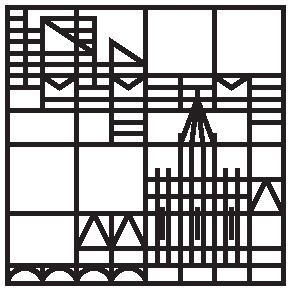
\includegraphics[width=5cm]{logo}
\\ \Large Universität Konstanz  \\ \vspace{4ex} \huge 
Skript zur Vorlesung\\ Höhere Quantentheorie und Elektrodynamik
\\ \vspace{4ex} \Large Prof. Dr. Wolfgang Belzig 
\\ Version vom 30. Juli 2012 \\ \vspace{4.5cm}
\normalsize Ursprünglichen Mitschrift von Birte Heinze im WS 09/10 \\ Ausführliche Überarbeitung von Tobias Lohse im WS 11/12 \vspace{-10cm}}
\author{}
\date{}
%\begin{document}

\subsection{Streutheorie}
Im folgenden Abschnitt soll die quantenmechanische Beschreibung von Streuprozessen näher beschrieben werden. Diese stellt einen der wichtigsten Anwendungsbereiche der Quantenmechanik dar, beispielsweise zur Bestimmung von Kernkräften oder Kristallstrukturen. Im Gegensatz  zu spektroskopischen Prozessen liegen bei Streuprozessen Anfangs- und Endzustand des betrachteten Systems im kontinuierlichen Teil des Eigenwertspektrums. Das gestreute Teilchen kommt aus dem Unendlichen in den Wirkungsbereich des Streukörpers, um nach dem Stoß asymptotisch detektiert zu werden. Es befindet sich also nicht in einem gebundenen Zustand. 

Im Gegensatz zur klassischen Streutheorie kann die Quantenmechanik nur  stochastische Aussagen über das Ergebnis der Ergebnis der Streuung machen. Insbesondere ist der Wirkungsquerschnitt des Streuprozesses, der sogenannte {\bf Streuquerschnitt}, interessant, welcher die Wahrscheinlichkeit angibt mit der ein Teilchen in einen bestimmten Raumwinkel $\Omega=(\vartheta,\varphi)$ gestreut wird. Der Streuquerschnitt kann direkt experimentell bestimmt werden, indem ein Teilchenstrahl auf den zu untersuchenden Streukörper gelenkt wird und mit einem Detektor der Teilchenstrahl nach der Streuung in allen Raumwinkeln abgetastet wird. Aus diesen Daten können dann Rückschlüsse auf die Struktur des Streukörpers gezogen werden, sofern der Zusammenhang zwischen dem Wirkungsquerschnitt und den elementaren Wechselwirkungspotentialen bekannt ist. Dieser Aufgabe wollen wir uns im folgenden zuwenden. 


\subsubsection{Streuung eines Wellenpakets}

Es soll zunächst die Ablenkung eines einlaufenden freien Teilchens, welches durch ein ebenes Wellenpaket beschrieben wird, an einem lokalisierten Potential beschrieben werden. Die folgende Abbildung soll diesen Prozess veranschaulichen: 
\vspace{-2ex}\begin{figure}[!h]\center
	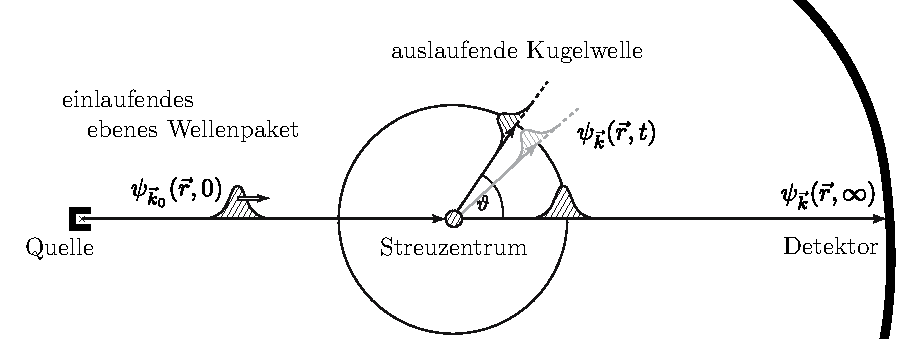
\includegraphics[scale=1]{Figs/Streuung}
\end{figure}\vspace{-4ex} 

Ein ebenes Wellenpaket $\psi_{\vec{k}_0}(\vec{r},0)$ mit Geschwindigkeit $\hbar\vec{k}_0/m$ trifft auf ein lokalisiertes Potential $\hat{V}$. Der Wechselwirkungsbereich dieses Potentials $\hat{V}(\vec{r})\neq0$ ist relativ klein, so dass wir es uns als relativ kleines Streuzentrum vorstellen können. Das Wellenpaket wechselwirkt nun also mit dem Potential und wird zu $\psi_{\vec{k}}(\vec{r},t)$, welches sich zusammensetzt aus einem Teil des Wellenpakets $\psi_{\vec{k}_0}(\vec{r},0)$ welches mit geringerer Intensität weiter läuft und einem anderer Teil, welcher asymptotisch als Kugelwelle beschrieben werden kann. Durch einen weit entfernten Detektor wird dann das Wellenpaket $\psi(\vec{r},\infty)$ detektiert. 

Das System wird durch den Hamiltonoperator $\hat{\ham}=-\hbar^2/2m\cdot\triangle + \hat{V}(\vec{r})$ beschrieben. Das einfallende Wellenpaket zur Zeit $t=0$ lässt sich wie folgt beschreiben:
\begin{eqnarray*}
	\psi_{\vec{k}_0}(\vec{r},0) &=& \int \frac{\mathrm{d} ^3k}{(2\pi)^3}\cdot \e^{\;\I\vec{k}\vec{r}}\cdot a_{\vec{k}} 
\end{eqnarray*}
Dabei haben die $a_{\vec{k}}$ ein Maximum bei $\vec{k}=\vec{k}_0$ und  $\e^{\;\I\vec{k}\vec{r}}$ sind die Eigenzustände des ungestörten Hamiltonoperators $\hat{\ham}_0=-\hbar^2/2m\cdot\triangle$ mit den Eigenwerten $E_{\vec{k}}=\hbar^2k^2/2m$. Die Eigenzustände $\psi_{\vec{k}}(\vec{r})$ des vollständigen Hamiltonoperators mit denselben Energien $E_{\vec{k}}$ sind durch die stationäre Schrödingergleichung (\ref{statSG}) bestimmt: 
\begin{eqnarray*}
	\Big(\frac{\hbar^2}{2m}\cdot\triangle + E_{\vec{k}}\Big)\;\psi_{\vec{k}}(\vec{r}) &=& \hat{V}(\vec{r})\;\psi_{\vec{k}}(\vec{r})
\end{eqnarray*}
Die Entwicklung des Eigenzustands $\psi_{\vec{k}_0}(\vec{r},0)$ nach $\psi_{\vec{k}}(\vec{r})$ liefert somit folgendes:
\begin{eqnarray*}
	\psi_{\vec{k}_0}(\vec{r},0) &=& \int \frac{\mathrm{d}^3 k}{(2 \pi)^3}\cdot \psi_{\vec{k}}(\vec{r})\cdot a_{\vec k}
\end{eqnarray*}
Wegen der asymptotischen Form $\e^{\;\I\vec{k}\vec{r}}$ der $\psi_{\vec{k}}(\vec{r})$ sind die $a_{\vec{k}}$ die selben für beide Darstellungen von $\psi_{\vec{k}_0}(\vec{r},0)$. Das heißt es kommen keine gebundenen Zustände vor, denn diese würden per Definition für $|\vec{r}| \to \infty$ verschwinden. 

Die Zustände zu einem beliebigen späteren Zeitpunkt $t>0$ ergeben sich für den zeitunabhängigen Hamiltonoperator direkt zu: 
\begin{eqnarray*}
	\psi(\vec{r},t) = \int \frac{d^3 k}{(2\pi)^3}\cdot\psi_{\vec{k}}(\vec{r})\cdot a_{\vec k} \cdot \e^{-\frac{\I}{\hbar}\cdot  E_{\vec{k}} t}
\end{eqnarray*}
Die Koeffizienten $a_{\vec{k}}$ sind dabei näherungsweise dieselben, wenn $\psi(\vec{r},0)$ vollständing außerhalb des Potentials liegt und $\psi_{\vec{k}}(\vec{r})\approx \e^{\I kr}$ gilt. 

Die Zeitentwicklung ist also mit der obigen Gleichung beschrieben, soll hier aber noch einmal anschaulich beschreiben werden. Nach der Streuung läuft einerseits das Wellenpaket mit geringerer Intensität weiter und andererseits läuft eine gestreute Kugelwelle aus, die jedoch eine winkelabhängige Amplitude besitzt.


\subsubsection{Formale Lösung der zeitunabhängigen Schrödingergleichung}\label{sec3.2}

Wir wollen nun die Form der $\psi_{\vec{k}}(\vec{r})$ bestimmen. Dazu müssen wir eine allgemeine Lösung der stationären Schrödingergleichung finden. Da das Potential in unserem Fall üblicherweise im Ortsraum nur eine einfache Funktion darstellt $\hat{V}(\vec{r})=V(\vec{r})$, hat die Gleichung die Form einer stationären Wellengleichung mit einer Inhomogenität: 
\begin{eqnarray}
	\Big( \frac{\hbar^2}{2m}\cdot \triangle + E_{\vec{k}}\Big)\;\psi_{\vec{r}}(\vec{r}) &=& V(\vec{r}) \cdot\psi_{\vec{k}}(\vec{r}) \label{statSGwelle}
\end{eqnarray}
Eine solche Gleichung lässt sich mit Hilfe der retardierten {\bf Greenschen Funktion} $G_{\vec{k}}(\vec{r}-\vec{r}\,')$ lösen. Die Greensche Funktion der Wellengleichung ist definiert als: 
\begin{eqnarray*}
	\Big( \frac{\hbar^2}{2m}\cdot\triangle + E_{\vec{k}}\Big)\; G_{\vec{k}}(\vec{r}- \vec{r}\,') &=& \delta(\vec{r} - \vec{r}\,')
\end{eqnarray*}
Diese Eigenwertgleichung ist mittels Fourier-Transformation einfach zu lösen. Es ergibt sich folgende explizite Darstellung der Greenschen Funktion:
\begin{eqnarray*}
	G_{\vec k}(r) &=& -\frac{m}{2\pi \hbar^2} \cdot \frac{e^{i k r}}{r}
\end{eqnarray*}
Die Greensche Funktion hat wie vermutet die Form einer auslaufenden Kugelwelle. Wir können somit die Gleichung (\ref{statSGwelle}) in eine Integralgleichung umschreiben:
\begin{eqnarray*}
	\psi_{\vec{k}}(\vec{r}) &=& \e^{\;\I\vec{k}\vec{r}} + \int\mathrm{d}^3 r'\; G(\vec{r}-\vec{r}\,')\cdot V(\vec{r}\,') \cdot\psi_{\vec{k}}(\vec{r}\,')
\end{eqnarray*}
Der Term $\e^{\;\I\vec{k}\vec{r}}$ ist die Lösung der homogenen Gleichung, er gewährleistet, dass die Anschlussbedingungen für asymptotisches Verhalten $|\vec{r}|\gg|\vec{r}\,'|$, erfüllt ist. In der Asymptotik gilt: 
\begin{eqnarray*}
	k \cdot |\vec{r}-\vec{r}\,'| = k \sqrt{r^2+r'\,^2-2\cdot\vec{r}\cdot\vec{r}\,'} \approx  k r \underbrace{\sqrt{1- \frac{2\cdot\vec{r}\cdot\vec{r}\,'}{r^2}}}_{\ll 1} \approx k r -\vec{k}_{\vec{r}}\vec{r}\,' \qquad \text{mit: } \vec k _{\vec r} = k \cdot \frac{\vec r}r
\end{eqnarray*}
Die folgende Skizze soll die Lage der Vektoren $\vec{k}$ und $\vec{k}_{\vec{r}}$ verdeutlichen. Wir können dabei $\vec{k}$ ohne Beschränkung der Allgemeinheit entlang der $z$-Achse legen: 
\begin{center}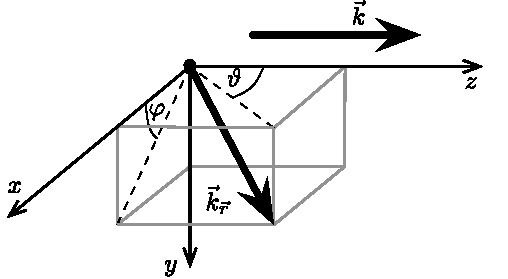
\includegraphics[scale=1]{Figs/kkr}\end{center}

Wir können somit die Welle $\psi_{\vec{k}}(\vec{r})$ in folgende Form umschreiben: 
\begin{eqnarray}
	\psi_{\vec{k}}(\vec{r}) = \e^{\;\I\vec{k}\vec{r}} + \frac{1}{r}\cdot f_{\vec{k}}(\vartheta,\varphi)\cdot\e^{\;\I kr} &\quad& \text{mit: } f_{\vec{k}}(\vartheta,\varphi) = -\frac{m}{2\pi\hbar^2} \int\mathrm{d}^3r'\;\e^{-\I\vec{k}_{\vec{r}}\;\vec{r}\,'}\cdot V(\vec{r}\,')\cdot \psi_{\vec{k}}(\vec{r}\,')\qquad\quad \label{streuzustand}
\end{eqnarray}
In dieser Form kann man nun gut erkennen, dass die ebene Welle hinter dem Streupotential mit geringerer Intensität weiterläuft und die gestreute Welle als Kugelwelle ausläuft, wobei die winkelabhängige Streuamplitude $f_{\vec{k}}(\vartheta,\varphi)$, die Information über das Potential enthält. Die Streuamplitude hängt dabei von der Richtung $(\vartheta,\varphi)$ der Beobachtung sowie von der Wellenlänge $\lambda=2\pi/k$ ab. Sie wird außerdem durch die exakten Lösung $\psi_{\vec k}(\vec r)$ der Schrödingergleichung bestimmt und hat die Dimension einer Länge. 


\subsubsection{Streuquerschnitt}

Wie bereits erwähnt ist der Streuquerschnitt eine wichtige Größe zur Beschreibung des Streuprozessen. Man Unterscheidet generell zwischen dem differentiellen und totalen Streuquerschnit. Der {\bf differentieller Streuquerschnitt} $\mathrm{d}\sigma/\mathrm{d}\Omega\;$ ist definiert als Quotient aus dem Strom der  pro Raumwinkel gestreuten Teilchen $\mathrm{d}I/\mathrm{d}\Omega$ und dem Betrag der Stromdichte der einfallenden Teilchen $j_{\text{ein}}$:
\begin{eqnarray*}
	\frac{\mathrm{d}\sigma}{\mathrm{d}\Omega} &=& \frac{\mathrm{d} I}{\mathrm{d}\Omega}\cdot\frac{1}{j_{\text{ein}}} \quad\!=\!\quad \frac{j_r\cdot r^2}{j_{\text{ein}}}
\end{eqnarray*}
Dabei ist $j_r$ der Betrag der Stromdichte der auslaufenden Kugelwelle. Zur Umformung wurde dabei die Kugelsymmetrie ausgenutzt, wegen der sich der infinitesimale Strom der ausfallenden Teilchen schreiben lässt als $\mathrm{d}I=\vec{j}_r\;\mathrm{d}\vec{A} = j_r\cdot r^2\;\mathrm{d}\Omega$. Die folgende Skizze soll die räumlichen Zusammenhänge etwas besser verdeutlichen: 
\vspace{-1ex}\begin{figure}[!h]\center
	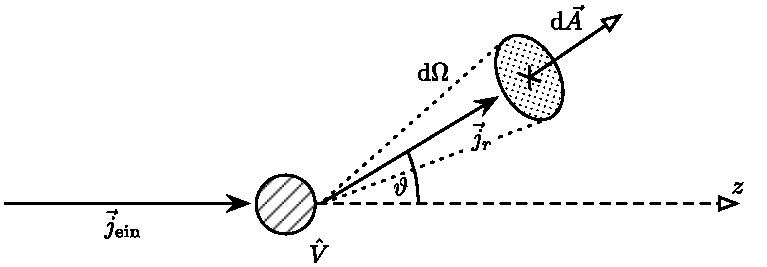
\includegraphics[scale=1]{Figs/DiffStreuQuer}
\end{figure}\vspace{-4ex} 

Die Stromdichte $j_{\text{ein}}$ der einfallenden Welle $\psi_{\vec{k}_0}(\vec{r},0)$ lässt sich berechnen zu:
\begin{eqnarray*}
	\vec{j}_{\text{ein}} &=& -\frac{\I\hbar}{2m}\cdot\big(\psi_{\vec{k}_0}^*\nabla\psi_{\vec{k}_0}-\psi_{\vec{k}_0}\nabla\psi_{\vec{k}_0}^*\big) \;=\; \frac {\hbar \vec{k}}{m}
\end{eqnarray*}
Der Betrag der Stromdichte $j_r$ der radial auslaufenden Kugelwelle $\psi_{\vec{k}}(r,t)\propto 1/r\cdot \e^{\;\I kr}$ ergibt sich dann zu: 
\begin{eqnarray*}
	j_r = -\frac{\I\hbar}{2m}\cdot\big|\psi_{\vec{k}}^*\nabla\psi_{\vec{k}}-\psi_{\vec{k}}\nabla\psi_{\vec{k}}^*\big| = \frac{\hbar}{m}\cdot \frac{k}{r^2}\cdot \big|f_{\vec{k}}(\vartheta, \varphi)\big|^2 = \frac{j_{\text{ein}}}{r^2}\cdot \big|f_{\vec{k}}(\vartheta, \varphi)\big|^2 
\end{eqnarray*}
Damit ergibt sich nun, dass der differentielle Streuquerschnitt $\mathrm{d}\sigma/\mathrm{d}\Omega$ das Betragsquadrat der Streuamplitude ist: 
\begin{eqnarray*}
\frac{\mathrm{d} \sigma}{\mathrm{d} \Omega} &=& \left | f_{\vec{k}}(\vartheta, \varphi) \ri|^2
\end{eqnarray*}
In der Asymptotik, kann außerdem der {\bf totalen Streuquerschnitt} $\sigma(\vec{k})$ angegeben werden, welcher ein Maß für die absolute Wahrscheinlichkeit einer Streuung der einfallenden Welle am Potential darstellt. Dieser ergibt sich wie folgt: 
\begin{eqnarray*} 
	\sigma(\vec{k}) &=& \int\mathrm{d}\Omega\; \big|f_{\vec k}(\vartheta,\varphi)\big|^2
\end{eqnarray*}
Der totale Streuquerschnitt ist ein Wirkungsquerschnitt und hat die Dimension einer Fläche. Er kann als 'Fläche' des Potentials vorgestellt werden, je größer diese ist, desto eher wird ein Teilchen an ihr gestreut. 


\subsubsection{Lösung des Radialteils der freien Schrödinger Gleichung}

Im folgenden soll die allgemeine Lösung der freien Schrödingergleichung noch einmal diskutiert werden. Die Eigenfunktionen der freien Schrödinger Gleichung in Kugelkoordinaten bestehen aus zwei Teilen: $\psi(r,\vartheta,\varphi) = R_l(r)\cdot Y_{lm}(\vartheta,\varphi)$. Die $Y_{lm}(\vartheta,\varphi)$ sind dabei die gut bekannten Kugelflächenfunktionen. Uns soll im folgenden der Radialteil $R_l(r)$ interessieren. Diese werden durch den Radialteil der freien Schrödingergleichung bestimmt, welcher folgende Form hat:
\begin{eqnarray*}
	\bigg( -\frac{\hbar^2}{2mr^2}\cdot \frac{\mathrm{d}}{\mathrm{d}r} \Big( r^2\cdot\frac{\mathrm{d}}{\mathrm{d}r} \Big) + \frac{\hbar^2 l(l+1)}{2mr^2} \bigg)\; R_l(r) &=& E\cdot R_l(r)
\end{eqnarray*}
Man definiert nun ein $\varrho=\sqrt{2mE/\hbar^2}\cdot r=kr$, mit dessen Hilfe man schreiben kann: 
\begin{eqnarray*}
\left( \frac{\mathrm{d}^2}{\mathrm{d}\varrho^2} + \frac{2}{\varrho}\cdot\frac{\mathrm{d}}{\mathrm{d}\varrho} + 1 + \frac{l(l+1)}{\varrho^2} \right) R_l(\varrho) &=& 0
\end{eqnarray*}
Diese Radialgleichung wird durch die sphärischen Bessel und Neumannfunktionen gelöst. Die sphärischen {\bf Besselfunktionen} $j_l(\varrho)$ haben folgende Eigenschaften: 
\begin{itemize1}
	\item Die Integraldarstellung der Besselfunktion ist folgende: 
	\begin{eqnarray*} 
		j_l(\varrho) &=& \frac{\varrho^l}{2^{l+1}l!}\cdot\int_{-1}^1 \!\!\mathrm{d}u\; \e^{\;\I\varrho u}(1-u^2)^l = \frac{1}{2\I^l} \cdot\int_{-1}^1\!\! \mathrm{d}u\; \e^{\I\varrho u} P_l(u)
	\end{eqnarray*}
	Dabei sind $P_l(u)$ die Legendre Polynome. 
	\item Die Besselfunktion ist am Ursprung regulär, für kleine $\varrho$ gilt also $j_l(\varrho)\propto \varrho^l$. 
	\item Das Asymptotische Verhalten ($\varrho\gg l$) der Besselfunktion ist gegeben durch: 
	\begin{eqnarray*}
		j_l(\varrho) &\approx& \frac{1}{\varrho} \cdot \sin\left(\varrho-\frac{\pi}{2} \cdot l \right)
	\end{eqnarray*}
\end{itemize1}

Die sphärischen {\bf Neumannfunktionen} $n_l(\varrho)$ haben folgende Eigenschaften: 
\begin{itemize1}
	\item Die Integraldarstellung der Neumannfunktion ist folgende: 
	\begin{eqnarray*} 
		n_l(\varrho) &=& j_{-(l+1)}(\varrho) = \frac{1}{2\I^{-(l+1)}} \cdot\int_{-1}^1\!\! \mathrm{d}u\; \e^{\;\I\varrho u} P_{-(l+1)}(u) 
	\end{eqnarray*}
	\item Die Neumannfunktion ist am Ursprung regulär, für kleine $\varrho$ gilt also $n_l(\varrho)\propto \varrho^{-(l+1)}$. 
	\item Das asymptotische Verhalten ($\varrho\gg l$) der Besselfunktion ist gegeben durch: 
	\begin{eqnarray*}
		n_l(\varrho) &\approx& -\frac{1}{\varrho} \cdot \cos\left(\varrho-\frac{\pi}{2} \cdot l \right)
	\end{eqnarray*}
\end{itemize1}

Die Allgemeine Lösung der Radialgleichung ist eine Überlagerung der sphärischen Bessel- und Neumannfunktionen: 
\begin{eqnarray*}
	R_{l,k}(r) &=& A_l\cdot j_l(kr)+B_l\cdot n_l(kr) 
\end{eqnarray*}
Jede Lösung der Schrödingergleichung muss sich also in Bessel- und Neumannfunktionen zerlegen lassen. Dies soll am Beispiel einer ebenen Welle gezeigt werden. Dazu wählen wir eine zur $z$-Achse rotationssymmetrische ebene Welle: $\vec{k}$ liegt also in $z$-Richtung. Für diese kommen nur Kugelflächenfunktionen  mit $m=0$ in Frage, welche die Form von Legendre Polynomen haben: $Y_{l0}=P_l(\cos\vartheta)$. Wir entwickeln die ebene Welle unter Verwendung der Definition $\varrho:=kr$ und $u:=\cos\vartheta$ in Legendre Polynomen: 
\begin{eqnarray*}
	\e^{\;\I \vec{k}\vec{r}} = \e^{\I kr\cos\vartheta}=\e^{\;\I\varrho u} &=& \sum_{l=0}^{\infty} b_l(\varrho)\cdot P_l(u)
\end{eqnarray*}
Wir suchen also die Koeefizienten $b_l(\varrho)$. Aus der Orthogonalität der Legendre Polynome folgt: 
\begin{eqnarray*}
	\int_{-1}^1 \!\!\mathrm{d}u\;\;P_l(u)\;P_{l'}(u)=\frac{2}{2l+1}\cdot\delta_{ll'} &\Rightarrow& b_l(\varrho) = (2l+1)\cdot\I^l \cdot j_l(\varrho)
	\\
	\Rightarrow \quad \e^{\;\I \vec{k}\vec{r}} &=& \sum_{l=0}^{\infty}(2l+1)\cdot\I^l \cdot j_l(\varrho) P_l(u)
\end{eqnarray*}



\subsubsection{Partialwellen-Zerlegung}
Falls $V(\vec{r})$ nur von $r$ abhängig ist, also ein Zentralpotential ist, so folgt aus der Rotationssymmetrie um die Einfallsachse, dass $f_{\vec{k}}(\vartheta,\varphi)$ nicht von $\varphi$ abhängt, sonder nur von $\vartheta$. 

Wir zerlegen zunächst die Streuamplitude $f_{\vec k}(\vartheta)$ nach Kugelflächenfunktionen $Y_{l0}=P_l(\cos\vartheta)$: 
\begin{eqnarray*}
	f_{\vec{k}}(\vartheta) &=& \sum_{l=0}^{\infty} (2l + 1)\cdot f_l(k)\cdot P_l(\cos{\vartheta})
\end{eqnarray*}
Die Koeffizienten $f_l(k)$ werden Partialwellenamplituden genannt. Wir betrachten nun die asymptotischen Streuzustände außerhalb des Potentials und entwicklen diese ebenfalls nach den Kugelflächenfunktionen $Y_{l0}$: 
\begin{eqnarray*}
	\psi_{\vec k}(\vec r) &=& \sum_{l=0}^{\infty} \I^l (2l + 1)\cdot R_l(r)\cdot P_l(\cos{\vartheta})
\end{eqnarray*}
Dabei sind $R_l(r)$ sind Lösungen der radialen Schrödingergleichung mit dem Potential $V(r)$ 

Die Streuzustände können aber asymptotisch ebenfalls wie in Gleichung (\ref{streuzustand}) als Überlagerung von ebener Welle und Kugelwelle mit Streuamplitude $f_{\vec{k}}(\vartheta)$ geschrieben werden. Wenn wir nun die ebenen Wellen und die Streuamplituden entwickeln und die Asymptotik der Besselfunktion benutzen, folgt aus dem Verglecih der beiden Darstellungen folgende asymptotische Form der $R_l(r)$: 
\begin{eqnarray*}
	R_l(r) &\approx& \I^lj_l(kr) + \frac{\e^{\;\I kr}}{r} f_l(k) \approx \frac 1 {2\I k} \Big( \big( 1 + 2\I k\cdot f_l(k) \big)\frac{\e^{\;\I kr}}r - \frac{\e^{-\I(kr-l\pi)}}r\Big)
\end{eqnarray*}
Der Effekt des Potentials ist somit eine Änderung des Vorfaktors der auslaufenden Kugelpartialwellen um den Vorfaktor $1+2\I k\cdot f_l(k) =: S_l(k)$, der als S-Matrix bezeichnet wird.

Aus der Unitarität folgt, dass Stromerhaltung gilt. Die einlaufende ist also gleich der auslaufenden Wahrscheinlichkeitsstromdichte. Mit dem Noethertheorem folgt aus der Rotationssymmetrie die Drehimpulserhaltung. Damit ist für jede Partialwelle der Betrag der einlaufenden Welle gleich dem der auslaufenden: $|S_l(k)|=1$. Der Effekt der Streuung ist somit eine reine Phasenverschiebung der auslaufenden Kugelwelle um eine sogenannte {\bf Streuphase} $\delta_l(k)$:  
\begin{eqnarray*}
	S_l = \e^{\;2\I\delta_l(k)} &\Rightarrow& R_l(r) \approx \frac 1 {2kr} \cdot\Big(\e^{\I(kr+2\delta_l(k))} - \e^{-\I(kr -l\pi)}\Big)
\end{eqnarray*}
Damit können wir nun die Partialwellenamplituden und somit auch die Streuamplitude in Abhängigkeit der Streuphase schreiben: 
\begin{eqnarray*}
	f_l(k) &=& \frac{1}{2\I k} \cdot\Big( \e^{\;2\I\delta_l(k)} -1\Big) = \frac{1}{k}\cdot \e^{\;\I\delta_l(k)}\cdot \sin\big(\delta_l(k)\big) \approx \frac{\delta_l(k)}{k}
	\\
	\Rightarrow\quad f_k(\vartheta) &=& \frac{1}{k} \cdot\sum_l (2l + 1)\cdot \e^{\I\delta_l(k)}\cdot \sin\big(\delta_l(k)\big)\cdot P_l(\cos\vartheta)
\end{eqnarray*}
Der Streuquerschnitt $\sigma(\vec{k})$ ergibt sich somit zu:
\begin{eqnarray*} 
	\sigma(k,\vartheta) &=& \int\mathrm{d}\Omega\; \big|f_k(\vartheta) \big|^2 = \int\mathrm{d}\Omega\; \sum_{ll'} (2l + 1)\cdot(2l' +1 )\cdot f_l f_{l'}\cdot P_l(\cos\vartheta)P_{l'}(\cos\vartheta) 
\end{eqnarray*}
Unter Ausnutzung der Orthogonalität der Legenre Polynome folgt dann: 
\begin{eqnarray} 
	\sigma(k,\vartheta) &=& 4 \pi \cdot\sum_{l} (2l + 1)\cdot |f_l|^2 = \frac{4\pi}{k^2}\cdot\sum_{l=0}^{\infty} (2l + 1)\cdot\sin^{2}\big(\delta_l(k)\big) \label{Streuquerschnit} 
\end{eqnarray}


\paragraph{Optisches Theorem}

Für den Imaginärteil der Partialwellenamplitude gilt:
\begin{eqnarray*}
	\Im\big(f_l(k)\big) = \frac{1}{k}\cdot\sin^2\big(\delta_l(k)\big) &\Rightarrow& \Im\big(f_k(\vartheta)\big) = \sum_{l = 0}^{\infty} (2l+1)\cdot \frac{1}{k}\cdot\sin^2\big(\delta_l(k)\big)\cdot P_l(\cos\vartheta)
\end{eqnarray*}
Für den Anteil der Welle, die das Potential auf gradem Weg durchläuft, aber trotzdem von diesem abgelenkt wird, ist $\vartheta=0$. Damit gilt für das Legendre Polynom $P_l(1) = 1$ und somit folgt aus Gleichung (\ref{Streuquerschnit}) folgende Darstellung für den Streuqueerschnitt:
\begin{eqnarray}
	\sigma(k,0) = \frac{4\pi}{k} \Im\big(f_k(0)\big) = \frac{4\pi}{k^2}\cdot\sum_{l=0}^{\infty}(2l+1)\cdot\sin^2\big(\delta_l(k)\big) \label{OptischesTheorem}
\end{eqnarray}
Diese Gleichung wird als optisches Theorem bezeichnet. Wir sehen also, dass die gesamte Amplitude des gestreuten Anteils der Abschwächung der Amplitude der durchgehenden Welle ($\vartheta = 0$) entspricht. Die Streuung hat ihr Maximum bei $\delta_l(k)=\pi/2+n\cdot\pi$ mit $n\in\mathbb{N}$, wo der Streuqueerschnitt einen Wert von $\sigma_l(k,0)=4\pi(2l+1)/k^2$ annimmt. $\sigma_l(k,0)$ hängt nicht mehr vom Potential ab, daher gilt das optische Theorem im Allgemein nicht nur für Zentralpotentiale. 



\subsubsection{Bornsche Näherung}

Wir haben bereits die allgemeine Bestimmungsgleichung für die Streuamplitude (\ref{streuzustand}) hergeleitet. Im Falle eines Zentralpotentials $V(r)$ können wir in diese Gleichung nun die Entwicklung der asymptotischen Streuzustände außerhalb des Potentials nach Kugelflächenfunktionen einsetzten. Wenn wir außerdem die Entwicklung von $\e^{\;\I \vec{k}\vec{r}}$ nach Kugelflächenfunktionen und die Orthogonalität der Kugelflächenfunktionen ausnutzen, ergibt sich folgende Gleichung für die Streuamplitude in Abhängigkeit von Legendre Polynomen $P_l$ und Besselfunktionen $j_l$: 
\begin{eqnarray*}
	f_k(\vartheta) &=& -\sum_{l = 0}^{\infty} (2l+1)\cdot P_l(\cos\vartheta)\cdot \underbrace{\frac {2 m}{\hbar^2}\cdot\int_0^{\infty}\!\! \mathrm{d}r\;r^2\cdot V(r) \cdot j_l(kr)\cdot R_l(r)}_{=\;-f_l(k)} 
\end{eqnarray*}
Für mit hoher Energie einfallende Teilchen und schwache Potentiale, die nur einen geringer Effekt auf $R_l$ haben, können wir die Näherung $R_l(r)\approx j_l(kr)$ machen. Außerdem wir für diesen Fall die Streuphase klein $\delta_l(k)\ll1$ und wir können die Partialwellenamplituden nach $\delta_l(k)$ entwickeln und enthalten folgende Darstellung der Streuphasen: 
\begin{eqnarray*}
	\delta_l(k) \approx k\cdot f_l = -\frac{2mk}{\hbar^2}\cdot \int_0^{\infty}\!\! \mathrm{d}r\; r^2\cdot V(r)\cdot j^2_l(kr)
\end{eqnarray*}
Diese Näherung wird als Bornsche Näherung der Streuphasen bezeichnet. Die Bornsche Näherung wird für große $l$ genau, also für Teilchen, die weit weg vom Streuer einfallen und wenig beeinflusst werden. 

Falls der Einfluss des Potentials auf alle Partialwellen klein ist,
so können wir in (\ref{streuzustand}) direkt die Näherung $\psi_{\vec{k}}(\vec{r})\approx\e^{\;\I\vec{k}\vec{r}}$ machen. Nach dieser Form der Bornschen Näherung ist die Streuamplitude dann proportional zur Fouriertransformierten des Potentials $\tilde{V}$: 
\begin{eqnarray*}
	f_{\vec{k}}(\vartheta,\varphi) &\approx& -\frac{m}{2\pi\hbar^2}\cdot \int \mathrm{d}^3r'\; \e^{\;\I(\vec{k}-\vec{k}_{\vec{r}})\vec{r}\,'}\cdot V(\vec{r}\,') \;\;=\; -\frac{m}{2\pi\hbar^2}\cdot \tilde{V}(\vec{k}_{\vec{r}}-\vec{k})
\end{eqnarray*}


\subsubsection{Streuung am Yukawa-Potential}

Wir wollen im folgenden die Streuung am sogenannten Yukawa-Potential betrachten, welches das Potential von massebehafteten Austauschteilchen darstellt und für starke Wechselwirkung und in Supraleitern eine Rolle spielt. Es wird auch als abgeschirmtes  Coulombpotential bezeichnet, da es für $\mu\to0$ in das Coulombpotential übergeht. Das Yukawa-Potenital hat folgende allgemeine Form: 
\begin{eqnarray*}
	V(r) = V_0 \frac{\e^{-\mu r}}{\mu r}
\end{eqnarray*}
Die Fouriertransformierte $\tilde{V}$ des Yukawa-Potentials lässt sich dann berechnen zu: 
\begin{eqnarray*}
	\tilde{V}(\vec{q}) &=& \frac{V_0}{2}\cdot \int\mathrm{d}^3r\; \e^{-\I\vec{q}\,\vec{r}}\cdot\frac{\e^{-\mu r}}{r} = \frac{4\pi}{q} \cdot \frac{V_0}{\mu}\cdot \int_0^{\infty} \mathrm{d}r\; \e^{-\mu r}\cdot \sin(qr) = \frac{4\pi}{\mu^2 + q^2} \cdot \frac{V_0}{\mu}
\end{eqnarray*}
In der obigen Umformung wurden dabei einige Schritte übersprungen, die uns aber an dieser Stelle nicht weiter interessieren sollen. 

Um die Streuamplitude in Bornscher Näherung zu berechnen, müssen wir $\tilde{V}(\vec{k}_{\vec{r}}-\vec{k})$ kennen. Wir finden dabei für $q^2=|\vec{q}|^2=|\vec{k}_{\vec{r}}-\vec{k}|^2$ mit Hilfe geometrischer Beziehungen, zu deren Veranschaulichung die Skizze in Abschnitt $\ref{sec3.2}$ hilfreich ist, folgende Darstellung: 
\begin{eqnarray*}
	q^2 &=& k_{\vec{r}}^2+k^2 - 2\cdot\vec{k}_{\vec{r}}\cdot\vec{k} = 2k^2\cdot(1-\cos\vartheta) = 4 k^2\cdot \sin^2(\vartheta/2)
\end{eqnarray*}
Damit ergibt sich für die Streuamplitude in Bornscher Näherung dann folgende Darstellung:
\begin{eqnarray*}
	|f_{\vec{k}(\vartheta)}| &=& - \frac{2m}{\hbar^2} \cdot V_0\cdot \frac{1}{4 k^2\cdot\sin^2(\vartheta/2)+\mu^2} 
\end{eqnarray*}
Im Grenzfall $\mu\to0$ für ein Coulombpotential mit $V_0/\alpha=q_1q_2/4\pi\varepsilon_0$ ergibt sich erstaunlicherweise obwohl die Voraussetzungen für die Bornsche Näherung nicht erfüllt sind der exakte Streuquerschnitt in Form der {\bf Rutherfordformel}: 
\begin{eqnarray*}
	\frac{\mathrm{d}\sigma}{\mathrm{d}\Omega} &=& \frac{(q_1q_2/4\pi\varepsilon_0)^2}{16E_k^2\cdot \sin^4(\vartheta/2)}
\end{eqnarray*}


\subsubsection{Resonanzstreuung am Potentialtopf}

Wir wollen zum Abschluss noch die Streuung an einem sphärischen Potentialtopf mit Radius $a$ und Potentialstärke $V_0$ betrachten: $V(r)=-V_0\cdot\Theta(a-r)$

Wegen der Kugelsymmetrie wird das Problem durch die radiale Schrödingergleichung mit der dimensionslosen Koordinate $\varrho=kr$ beschrieben:
\begin{eqnarray*}
	\bigg( \frac{\mathrm{d}^2}{\mathrm{d}\varrho^2} + \frac{2}{\varrho}\frac{\mathrm{d}}{\mathrm{d}\varrho} - \frac{l(l+1)}{\varrho^2} + \frac{2m\big(E-V(\varrho)\big)}{\hbar^2k^2} \bigg)\;R_l(\varrho) &=& 0
\end{eqnarray*}
Mit der Energie $E=\hbar^2k^2/2m$. Für ein konstantes Potential ändert sich nur der Wellenvektor und die linear unabhängigen Lösungen sind immer noch durch die sphärischen Bessel und Neumann Funktionen: 
\begin{eqnarray*}
	j_l(\varrho) = (-\varrho)^l \cdot\left(\frac{1}{\varrho}\frac{\mathrm{d}}{\mathrm{d}\varrho}\ri)^l\cdot\frac{\sin(\varrho)}{\varrho} &\quad& n_l(\varrho) = -(-\varrho)^l \cdot\left(\frac{1}{\varrho}\frac{\mathrm{d}}{\mathrm{d}\varrho}\ri)^l\cdot\frac{\cos(\varrho)}{\varrho}
\end{eqnarray*}
Für $l=0$ ergeben sich also $j_0(\varrho)=\sin\varrho/\varrho$ und $n_0(\varrho)=-\cos\varrho/\varrho$. Und als allgemeine Lösung ergibt sich unter der Bedingung, dass die Lösung für $r=0$ regulär sein soll für $r<a$ zu $R_l(r)=A_l\cdot j_l(k'r)$ und für $r\geq a$ zu $R_l=B_l\cdot j_l(kr)+C_l\cdot n_l{kr}$. Dabei ist der Wellenvektor für $r<a$ gegeben durch $k'=\sqrt{2m(E+V_0)/\hbar^2}$ und für $r\geq a$ durch $k=\sqrt{2mE/\hbar^2}$. Die Koeffizienten $A_l$, $B_l$ und $C_l$ ergeben sich dabei aus der Stetigkeitsbedingung für $R_l(r)|_{r=a}$ und $\dell_r R_l(r)|_{r=a}$ als Funktionen der Streuphase. 

In der Asymptotik $r\to\infty$ dominiert für langsame Teilchen $ka\ll1$ gilt $\tan\delta_l\ll1$ und somit dominiert die $s$-Welle $l=0$, deren Steuphase gegeben ist durch $\tan\delta_0=-C/B$. Die Eigenfunktionen ergeben sich dann als: 
\begin{eqnarray*}
	R_l(r) &\approx& B_0\cdot j_0(kr) + C_0 \cdot n_0(kr) = \frac B{kr}\cdot\Big(\sin(kr)-\frac{C}{B}\cdot\cos(kr) \Big) = \frac{B}{kr}\cdot\frac{\sin(kr + \delta_0)}{\cos(\delta_0)} 
\end{eqnarray*}
Für langsamen Teilchen liegt also auch im Fall des Potentialtopfs eine isotrope $s$-Streuung vor, wie bei der Streuung an einer harten Kugel mit Radius $a$. 

Im allgemeinen $l\neq0$ kann die Streuphase beliebige Werte annehmen. Ein Maximum nimmt der partielle Streuquerschnitt nach dem optischen Theorem für Werte $\delta_l \approx\pi/2+n\pi$ mit $n\in \mathbb{N}$ an, hier gilt: 
\begin{eqnarray*}
	\sigma_l = \frac{4\pi}{k^2}\cdot (2l +1)\cdot \underbrace{\sin^2(\delta_l)}_{=1}
\end{eqnarray*}
Diese Maxima von $\sigma_l$ treten auf, wenn die Energie in den Bereich der sogenannten Resonanzenergie $E_R$ kommt. Für den Fall eines tiefen und schmalen Potentialtopfs $k'a\gg l$ entspricht diese Energie der Energie eines gebundenen Zustands im tiefen dreidimensionalen Potentialtopf. Wir sprechen in diesem Fall von {\bf Resonanzstreuung}, da hier quasi gebundene Zustände auftreten. Da im Bereich der Potentialstreuung wegen $\tan\delta_l\ll1$ gilt $\delta_l\approx n\pi$, muss offensichtlich $\delta_l(E)$ bei $E_R$ einen Sprung haben. Das Problem lässt sich somit durch ein effektives Potential $V_{\text{eff}}$ beschreiben, welches in etwa folgende Form hat: 
\begin{figure}[!h]\center
	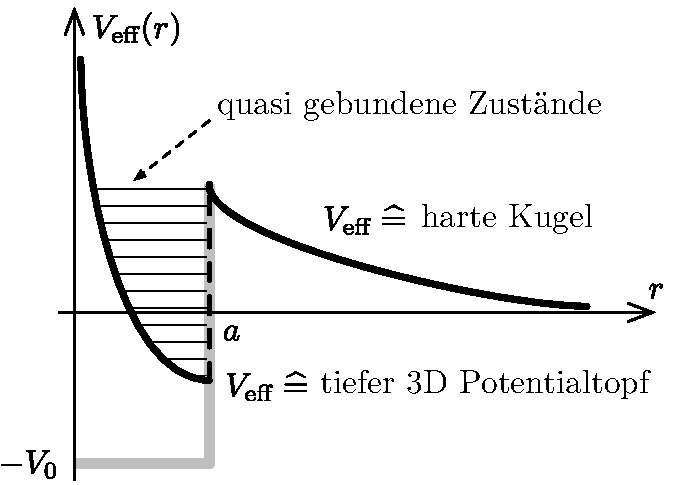
\includegraphics[scale=0.75]{Figs/Veff} 
\end{figure}\vspace{-4ex} 

In linearer Näherung gilt in der Nähe von $E_R$: $\cot(\delta_l)\approx E-E_R/\Gamma_l$. Wobei $\Gamma_l$ einen hier nicht näher bestimmten Faktor darstellt, welcher von der Resonanzenergie $E_R$ abhängt. Es lässt sich damit dann die sogenannte \textbf{Breit-Wigner-Formel} für die partiellen Streuquerschnitte herleiten: 
\begin{eqnarray*}
	\sigma_l(E) &=& \frac{4\pi(2l+1)}{k^2}\cdot \frac{(\Gamma_l/2)^2}{(E-E_r)^2+(\Gamma_l/2)^2}
\end{eqnarray*}
Der totale Streuquerschnitt $\sigma$ ergibt sich dann als $\sigma=\sum_l\sigma_l$. 

%\end{document} \newpage
\thispagestyle{plain} %\documentclass[a4paper,12pt,final,twoside]{scrartcl}
\setcounter{secnumdepth}{3}
\setcounter{tocdepth}{5}

\usepackage[utf8]{inputenc}
\usepackage[T1]{fontenc}
\linespread{1.4}
\usepackage{dsfont}
\usepackage{amsfonts}
\usepackage{amsmath}
\usepackage{amssymb}
\usepackage{amsthm}
\usepackage{mathtools}
\usepackage{mathbbol}
\usepackage{amsmath1}
\usepackage[ngerman]{babel}
\usepackage{bibgerm}
\usepackage[pdftex]{graphicx}
%\usepackage{mathpazo}
\usepackage{floatflt}
%%\usepackage{epsfig}
\usepackage{wrapfig}
\usepackage{graphicx}
\usepackage{tabularx}
\usepackage{caption} 
\usepackage{multicol} 
\usepackage{mathrsfs}
%\usepackage{pspicture}
%\usepackage{eepic}
%\usepackage{epic}
%\usepackage{trfsigns}

%\usepackage[ansinew]{inputenc}
\usepackage{longtable,array,dcolumn}
%\usepackage{ngerman}
\usepackage{epic}
\usepackage{rotate}
\usepackage{graphpap}
\usepackage{amssymb}
\usepackage[squaren]{SIunits}
\usepackage{curves}
\usepackage{float}
\usepackage{array}
\usepackage{enumerate}
\usepackage{marvosym}
\usepackage{slashed}%für feynmanslsash
\usepackage[breaklinks,pdfborder={0 0 0}]{hyperref}
\usepackage{ulem}	%angeblich funktioniert dann
\let\underbar\uline	%underbar in math auch bei greek letters
\usepackage{multirow}
%\usepackage{multicolumn}
\usepackage{enumitem}


\setlength{\parskip}{12pt}
\setlength{\parindent}{0mm}
%\newcommand{\grad}{\ensuremath{^{\circ}}
%\renewcommand{\figurename}{Abb.}		% mit usepackage caption2
%\renewcommand{\captionfont}{\small \itshape}	% mit usepackage caption2
%\setkomafont{caption}{\small \itshape}		%sollte mit caption im userpackage funktionieren
%\setkomafont{captionlabel}{\small , \itshape}	%sollte mit caption im userpackage funktionieren
\captionsetup{font = {small, sf}} %mit it anstelle von sf gibts kusiv

\date{2009-20-10}
\newcommand{\kreis}[1]{
 \qbezier(-#1,0)(-#1,#1)(0,#1)
  \qbezier(0,#1)(#1,#1)(#1,0)
  \qbezier(#1,0)(#1,-#1)(0,-#1)
  \qbezier(0,-#1)(-#1,-#1)(-#1,0)}
\newcommand{\s}{\ \big| \ }
\newcommand{\lo}{\left <}
\newcommand{\ro}{\ri >}
\newcommand{\g}{&=&}

\newcommand{\ham}{\mathcal H}
\newcommand{\hil}{\mathscr H}
\newcommand{\fok}{\mathscr F}
\newcommand{\wh}{\widehat}
%\newcommand{\left}{\left}
\newcommand{\ri}{\right}
\newcommand{\Sp}{\text{Sp}}
\newcommand{\babsatz}{\par \begingroup \leftskip=2cm}
\newcommand{\eabsatz}{\par\endgroup}

\newcommand{\D}{\text{\itshape D}}
\newcommand{\Lr}{\mathcal L }%\textit{L}}
\newcommand{\rot}{\text{rot}}
\newcommand{\divergenz}{\text{div}}
\newcommand{\grad}{\text{grad}}
\newcommand{\grat}{${}^{\circ}$}
%\newcommand{\tanh}{\text{tanh}} already defined

\newcommand{\RM}[1]{\text{\MakeUppercase{\romannumeral #1}}}
\newcommand{\dell}{\partial}
\renewcommand{\div}{\operatorname{div}}
\newcommand{\I}{\dot{\text{\i\!\i}}}
\newcommand{\e}{\mathrm{e}}
\newcommand{\ket}[1]{\mid\!\!\!\,\,{#1}\rangle}
\newcommand{\bra}[1]{\langle{#1}\!\!\!\,\,\mid}
\newcommand{\braket}[2]{\langle{#1}\!\!\!\,\,\mid\!\!\!\,\,{#2}\rangle}
\newcommand{\bracket}[3]{\langle{#1}\!\!\!\,\,\mid\!\!\!\,\,{#2}\!\!\!\,\,\mid\!\!\!\,\,{#3}\rangle}
\newcommand{\1}{\mathds{1}}
\newcommand{\EW}[1]{\langle\!\!\,\,#1\!\!\,\,\rangle}
\newcommand{\arrowbox}[1]{-\!\!\!\!\:\text{(#1)}\!\!\!\;\;\!\!\!\rightarrow}

\newcommand{\ketI}[1]{\ket{#1}_{\!\!\;\text{I}}}
\newcommand{\ketII}[1]{\ket{#1}_{\!\!\;\text{II}}}
\newcommand{\ketIII}[1]{\ket{#1}_{\!\!\;\text{III}}}
\newcommand{\braI}[1]{\,\!_{\text{I}\!\!\;}\bra{#1}}
\newcommand{\braII}[1]{\,\!_{\text{II}\!\!\;}\bra{#1}}
\newcommand{\braketI}[2]{\,_{\text{I}\!\!\;}\braket{#1}{#2}_{\!\!\;\text{I}}\,}
\newcommand{\braketII}[2]{\,_{\text{II}\!\!\;}\braket{#1}{#2}_{\!\!\;\text{II}}\,}
\newcommand{\braketIII}[2]{\,_{\text{III}\!\!\;}\braket{#1}{#2}_{\!\!\;\text{III}}\,}
\newcommand{\bracketI}[3]{\,_{\text{I}\!\!\;}\bracket{#1}{#2}{#3}_{\!\!\;\text{I}}\,}
\newcommand{\bracketII}[3]{\,_{\text{II}\!\!\;}\bracket{#1}{#2}{#3}_{\!\!\;\text{II}}\,}


\newcommand{\up}{\ket{\uparrow}}
\newcommand{\updg}{\bra{\uparrow}}
\newcommand{\down}{\ket{\downarrow}}
\newcommand{\downdg}{\bra{\downarrow}}
\newcommand{\upup}{\ket{\uparrow\uparrow}}
\newcommand{\updown}{\ket{\uparrow\downarrow}}
\newcommand{\downup}{\ket{\downarrow\uparrow}}
\newcommand{\downdown}{\ket{\downarrow\downarrow}}

\newenvironment{itemize1}{\begin{itemize}[leftmargin=5mm,itemsep=-1ex,topsep=-1ex]}{\end{itemize}}

%\usepackage[left=2cm,right=2cm,top=1cm,bottom=1cm,includeheadfoot]{geometry}

\usepackage{fancyhdr}
\pagestyle{fancy}{\fancyhf{}
\fancyhead[LO,RE]{\footnotesize \rightmark}
\fancyfoot[C]{\footnotesize -$\,$\thepage$\;$-}
\renewcommand{\headrulewidth}{0.4pt}
\renewcommand{\footrulewidth}{0pt}}

\fancypagestyle{plain}{\fancyhf{}
\renewcommand{\headrulewidth}{0.4pt}
\fancyfoot[C]{\footnotesize -$\,$\thepage$\,$-}}

\usepackage{titlesec}
\titleformat{\section}[display]{\sffamily\bfseries\Huge\center}{Kapitel \thetitle:}{1ex}{}{}
\newcommand{\kapitel}[2]{$\;$\vspace{-1.5cm} \section[#1]{#2} \rule{17cm}{0.4pt}\vspace{3cm}}
\titleformat{\paragraph}[hang]{\sffamily\bfseries}{\thetitle:}{0ex}{\vspace{-0.15cm}}{\vspace{0.5cm}}

\title{ \vspace{1.5cm}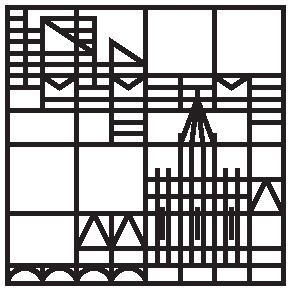
\includegraphics[width=5cm]{logo}
\\ \Large Universität Konstanz  \\ \vspace{4ex} \huge 
Skript zur Vorlesung\\ Höhere Quantentheorie und Elektrodynamik
\\ \vspace{4ex} \Large Prof. Dr. Wolfgang Belzig 
\\ Version vom 30. Juli 2012 \\ \vspace{4.5cm}
\normalsize Ursprünglichen Mitschrift von Birte Heinze im WS 09/10 \\ Ausführliche Überarbeitung von Tobias Lohse im WS 11/12 \vspace{-10cm}}
\author{}
\date{}
%\begin{document}

\subsection{Quantendynamik mit Propagatoren}
Im folgenden Abschnitt soll auf die Beschreibung der Dynamik quantenmechanischer Systeme mittels sogenannter Propagatoren eingegangen werden, welche schließlich auf die Pfadintegralformilierung der Quantenmechanik nach Feynman führt. 

\subsubsection{Propagatoren und die Greensche Funktion der Schrödingergleichung}
Wir wollen uns im folgenden mit der allgemeinen Lösung der Schrödingergleichung (\ref{SGL}) für einen zeitunanbhängigen Hamiltonoperator $\hat{\ham}$ im Ortsraum beschäftigen. 

Die Basis des Ortsraum besteht aus den Zuständen $\ket{x}$ mit $x\in\mathbb{R}$, ist also unendlich dimensional. Die Orthonormalität der Ortszustände wird dann mit der Deltafunktion notiert: $\braket{x}{x'}=\delta(x-x')$. Der Ket-Vektor $\ket{\psi}$ kann im Ortsraum geschrieben werden als Wellenfunktion: $\braket{x}{\psi(t)}=\psi(x,t)$. Die Lösung der Schrödingergleichung für einen zeitunabhängigen Hamiltonoperator ergibt sich, wie wir bereits gezeigt haben zu: 
\begin{eqnarray*} 
	\ket{\psi(t)} &=& \e^{-\frac{\I}{\hbar}\cdot \hat{\ham}\cdot(t-t')}\; \ket{\psi(t')}
\end{eqnarray*} 
Wenn wir in diese Gleichung eine $\1=\int \mathrm{d}x\;\ket{x}\bra{x}$ einfügen und beide Seiten von links mit $\bra{x}$ multiplizieren, so ergibt sich:
\begin{eqnarray}
	\braket{x}{\psi(t)} &=& \int\mathrm{d}x'\; \underbrace{\bracket{x}{\e^{-\frac{\I}{\hbar}\cdot\hat{\ham}\cdot(t-t')}}{x'}}_{=:\;K(x,t,x',t')} \cdot \braket{x'}{\psi(t)} \nonumber
	\\
	\Leftrightarrow\qquad \psi(x,t) &=& \int\mathrm{d}x'\; K(x,t,x't') \cdot\psi(x',t') \label{PropagatorDynamik}
\end{eqnarray}
Die Funktion $K(x,t,x',t')$ wird dabei als {\bf Propagator} bezeichnet. Die Bestimmung des Propagators ist somit äquivalent zur Lösung der zeitabhängigen Schrödingergleichung. Der Propagator beschreibt die Amplitude am Ort $x$ zur Zeit $t$, die von der Ausgangsamplitude bei $x'$ zur Zeit $t'$ verursacht wird. Der Endzustand ergibt sich also als Superposition der Anfangszustände mit Amplitudengewichtung $K(x,t,x',t')$. Der Propagator selbst erfüllt die Schrödingergleichung:
\begin{eqnarray*} 
	\I\hbar\cdot\dell_t\;K(x,t,x',t') = \hat{\ham}\;K(x,t,x',t') &\quad& \text{mit Anfangsbedingung: } K(x,t,x',t) = \delta(x-x')
\end{eqnarray*} 
Der Propagator hat somit eine gewisse Ähnlichkeit mit einer Greenschen Funktion. Und tatsächlich können wir mit seiner Hilfe leicht eine {\bf retardierte Greensche Funktion} $G_R(x,t,x',t')$ und eine {\bf avancierte Greensche Funktion} $G_A(x,t,x',t')$ der Schrödingergleichung einführen: 
\begin{eqnarray*}
	G_R(x,t,x't') = -\frac{\I}{\hbar}\cdot\Theta(t-t')\cdot K(x,t,x',t')
	\\
	G_A(x,t,x't') = \frac{\I}{\hbar}\cdot\Theta(t'-t)\cdot K(x,t,x',t')
\end{eqnarray*}
Die unterschiedlichen Theta-Funktionen sorgen dafür, dass die retardierte Greensche Funktion nur für kausale Zusammenhänge ungleich 0 ist und die avancierte nur für antikausale. In der Physik wird Kausalität dabei verstanden als zeitliche Abfolge von Zusammenhängen, deren Propagation eindeutig positiv bestimmt ist. 

Wenn wir die retardierte oder avancierte Greensche Funktion in die Schrödingergelichung einsetzten, lässt sich zeigen, dass es sich bei den von uns definierten Funktionen tatsächlich um Greensche Funktionen handelt: 
\begin{eqnarray*}
	\I\hbar\cdot\partial_t\; G_{R/A}(x,t,x',t') &=& \I\hbar \frac{\mp\I}{\hbar}\Big(K(x,t,x',t')\cdot\underbrace{\partial_t\;\Theta(\pm t\mp t')}_{=\;\delta(\pm t\mp t')} + \Theta(\pm t\mp t')\cdot\underbrace{\partial_t\; K(x,t;x',t')}_{= \hat{\ham}\;K(x,t,x',t')/\I\hbar}\Big)
	\\
	&=& \pm\Big(\underbrace{K(x,t,x',t)}_{=\;\delta(x-x')}\cdot\delta(t-t')\pm\hat{\ham}\;\underbrace{\frac{\mp\I}{\hbar}\cdot\Theta(\pm t\mp t')\cdot K(x,t,x',t')}_{=\;G_{R/A}(x,t,x',t')}\Big) 
	\\\;\\
	\Leftrightarrow\quad \big(\I\hbar\partial_t-\hat{\ham}\big)\; G_{R/A}(&&\!\!\!\!\!\!\!\!\!\!\!\!\!\!x,t,x',t') \;\;=\;\; \delta(x-x')\cdot\delta(t-t') 
\end{eqnarray*}
Wegen der Zeitumkehrinvarianz der Schrödingergleichung ist diese jedoch nicht hinreichend um die Greensche Funktion zu definieren, da sie keine Unterscheidung zwischen retardierter und avancierter Greenscher Funktion zulässt. 

Da die Greensche Funktion eine inhomogenen Differentialgleichungung erfüllt, ist sie im Fourierraum sehr leicht lösbar und ist somit bei der allgemeinen Lösung von Problemen hilfreich sein. 


\subsubsection{Greensche Funktion eines freien Teilchens}

Im folgenden wollen wir die Verwendung und Bestimmung der Greenschen Funktion am Beispiel eines freien Teilchens mit dem Hamiltonoperaotr $\hat{\ham}=-\triangle/2m$ erläutern. 

Die Fouriertransformierte der Greenschen Funktion $\tilde{G}(\omega,k)$ lässt sich leicht bestimmen und ist gegeben durch: 
\begin{eqnarray*}
	\widetilde{G}(\omega,k) \;\;=\;\; \frac{2m}{\omega-\hbar^2k^2} &=& \frac{1/\hbar}{\omega-\omega(k)} \quad\qquad\text{mit: } \omega(k) = \frac{\hbar k^2}{2 m} 
\end{eqnarray*}
Die Greensche Funktion ist dann bestimmt durch die Rücktransformation, welche sich als folgendes Integral schreiben lässt: 
\begin{eqnarray*}
	G(x,t,0,0) &=& \int\frac{\mathrm{d}\omega}{2\pi}\int\frac{\mathrm{d}k}{2\pi}\;\e^{\;\I(kx-\omega t)}\cdot \widetilde{G}(\omega,k)
\end{eqnarray*}
Allerdings besteht das Problem, dass die Fouriertransformierte Greensche Funktion $\tilde{G}$ singulär für $\omega(k)=\omega$ ist, sodass die Kausalität in diesem Fall unklar ist. Dies können wir lösen, indem wir die Frequenz $\omega$ um einen imaginären  Parameter verschieben und dann diesen Parameter gegen Null gehen lassen. 
\begin{eqnarray*} 
	\widetilde{G}_{R/A}(\omega,k) = \lim_{\delta\to0}\;\widetilde{G}(\omega\pm\I\delta,k)
\end{eqnarray*} 
Wir wollen uns zunächst mit dem Integral über $\mathrm{d}\omega$ für die Greensche Funktion beschäftigen: 
\begin{eqnarray*}
	\tilde{G}_{R/A}(t,k) &=& \lim_{\delta\to0}\;\;\frac{1}{\hbar}\cdot \int_{-\infty}^{+\infty}\!\!\!\mathrm{d}\omega\;\underbrace{\frac{\e^{-\I\omega t}/2\pi}{\omega-(\omega(k)\mp\I\delta)}}_{:=\;g_{R/A}(\omega)}
\end{eqnarray*}
Zur Berechnung dieses Integral können wir den {\bf Residuensatz} verwenden: 
\begin{eqnarray*}
	\oint_{\gamma}\mathrm{d}s\;f = 2\pi\I\cdot\sum_n\mathrm{ind}_{z_n}\cdot\text{Res}_f(z_n) \qquad\text{Pol erster Ordnung: } \text{Res}_f(z_0)=\lim_{z\to z_0}\;(z-z_0)\cdot f(z)
\end{eqnarray*}
Dabei sind $z_n$ die Polstellen der Funktion $f$ und $\mathrm{ind}_{z_n}$ die Windungszahlen der Polstelle. Wir wandeln das Integral dazu in eine Kurvenintegral in der komplexen Ebene von $\omega=|\omega|\cdot\e^{\;\I\varphi}$ um und lassen dann $|\omega|$ gegen unendlich gehen. Die folgende Skizze soll dies verdeutlichen: 
\begin{figure}[h!]\centering
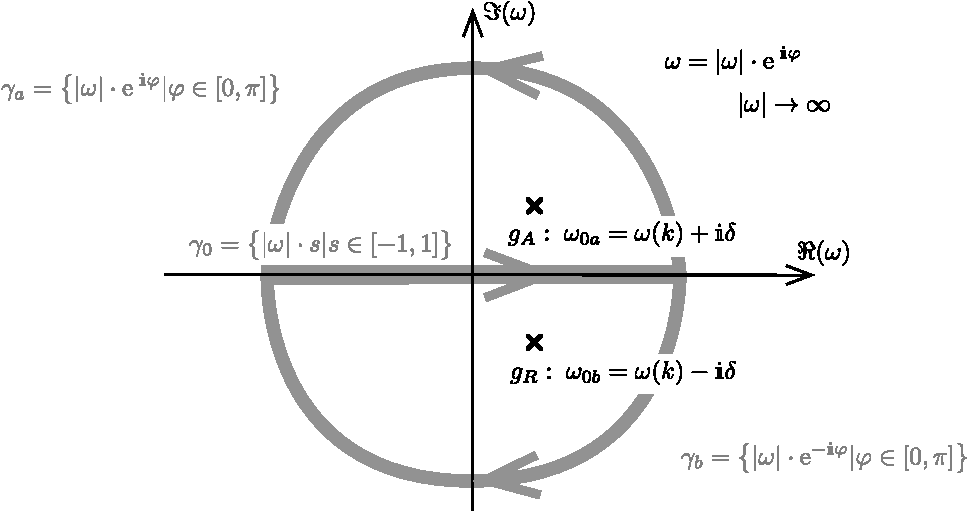
\includegraphics[scale=1]{Figs/komplexeebene}
\end{figure}

Wir erweitern den Integrationsweg $\gamma_0$ also um den oberen Integrationsweg $\gamma_a$ beziehungsweise den unteren Integrationsweg $\gamma_b$, um ein geschlossenes Kurvenitegral zu erhalten. Dies ist möglich, sofern für $|\omega|\to\infty$ dieses zusätzliche Kurvenintegral verschwindet. Ob das Integral über $\gamma_a$ beziehungsweise $\gamma_b$ verschwindet hängt dabei davon ab, ob die Zeit negativ oder positiv ist. Es lässt sich zeigen, dass gilt: 
\begin{eqnarray*}
	t>0:&\;&\int_{\gamma_a}\!\!\!\mathrm{d}s\; g_{R/A}=\int_0^{\pi}\!\!\!\mathrm{d}\varphi\;g_{R/A}\big(|\omega|\cdot\e^{\;\I\varphi}\big)\cdot|\omega|\;\underset{|\omega|\to\infty}{\to}\;\infty \qquad\land\qquad \int_{\gamma_b}\!\!\!\mathrm{d}s\; g_{R/A}\;\underset{|\omega|\to\infty}{\to}\;0
	\\\;\\
	t<0:&\;&\int_{\gamma_a}\!\!\!\mathrm{d}s\; g_{R/A}\;\underset{|\omega|\to\infty}{\to}\;0 \qquad\land\qquad \int_{\gamma_b}\!\!\!\mathrm{d}s\; g_{R/A}=\int_0^{\pi}\!\!\!\mathrm{d}\varphi\;g_{R/A}\big(|\omega|\cdot\e^{-\I\varphi}\big)\cdot|\omega|\;\underset{|\omega|\to\infty}{\to}\;\infty
\end{eqnarray*}
Wir können somit für $t>0$ den geschlossenen Integrationsweg $\gamma_0+\gamma_b$ wählen und für $t<0$ den geschlossenen Integrationsweg $\gamma_0+\gamma_a$. Wir müssen nun noch das Residuum für die beiden Integrationswege an den Polstellen der Funktionen $g_{R/A}$ berechnen. Dabei hat $g_R$ eine Polstelle bei $\omega_{0b}=\omega(k)-\I\delta$, die auf Weg $\gamma_0+\gamma_a$ nicht umlaufen wird und auf Weg $\gamma_0+\gamma_b$ mit Windungszahl $\mathrm{ind}_{\omega_0}=-1$ umlaufen wird. $g_A$ hat eine Polstelle bei $\omega_0=\omega(k)+\I\delta$, die auf Weg $\gamma_0+\gamma_a$ mit Windungszahl $\mathrm{ind}_{\omega_{0a}}=1$ umlaufen wird und auf Weg $\gamma_0+\gamma_b$ nicht umlaufen wird. Wir sehen somit, dass die Kausalität beziehungsweise Antikausalität für die retardierte undavancierte Greensche Funktion gewährlesitet ist. Es ergibt sich dann $\tilde{G}_{R/A}(t,k)$ zu: 
\begin{eqnarray*}
	\oint_{\gamma_0+\gamma_a}^{(t<0)}\!\!\!\!\!\!\!\!\!\mathrm{d}s\;g_A = 2\pi\I\cdot\text{Res}_{g_A}(\omega_{0a})= \lim_{\omega\to\omega_{0a}}\;\I\cdot\e^{-\I\omega t}\;=\;\I\cdot\e^{-\I(\omega(k)+\I\delta)t}\;\land\; \oint_{\gamma_0+\gamma_b}^{(t>0)}\!\!\!\!\!\!\!\!\!\mathrm{d}s\;g_R = -\I\cdot\e^{-\I(\omega(k)-\I\delta)t}
	\\
	\land\;\oint_{\gamma_0+\gamma_b}^{(t>0)}\!\!\!\!\!\!\!\!\!\mathrm{d}s\;g_A = \oint_{\gamma_0+\gamma_a}^{(t<0)}\!\!\!\!\!\!\!\!\!\mathrm{d}s\;g_R = 0 \qquad\Rightarrow\qquad\qquad \tilde{G}_{R/A}(t,k) = \mp\frac{\I}{\hbar}\cdot\Theta(\pm t)\cdot \e^{-\I\omega(k) t} \qquad\qquad
\end{eqnarray*}
Es bleibt noch das Integral über $\mathrm{d}k$ zu bestimmen. Dieses hat nun folgende Form: 
\begin{eqnarray*}
	G_{R/A}(t,x) &=& \mp \frac{\I}{\hbar}\cdot\Theta(\pm t)\cdot\int_{-\infty}^{+\infty}\frac{\mathrm{d}k}{2\pi}\; \e^{\I(kx-\omega(k)t)} 
\end{eqnarray*}
Der Exponent der e-Funktion im Integral kann dabei so umgeformt werden, dass sich ein Fresnelintegral ergibt, welches sich leicht lösen lässt: 
\begin{eqnarray} 
	&&\!\!\!\! \I\cdot\big(kx-\omega(k)t\big) = \I\cdot\Big(kx-\frac{\hbar k^2}{2m}t\Big) = -\I\cdot\underbrace{\frac{\hbar t}{2m}\cdot\Big(k-\frac{mx}{\hbar t}\Big)^2}_{=:\;u^2} +\I\cdot\underbrace{\frac{\hbar t}{2m}\cdot\frac{m^2x^2}{\hbar^2t^2}}_{=\; mx^2/2\hbar t\;=:\;d} = -\I\cdot(u^2-d) \nonumber
	\\\;\nonumber\\
	\Rightarrow&&\!\!\!\!\int_{-\infty}^{+\infty}\frac{\mathrm{d}k}{2\pi}\; \e^{\I(kx-\omega(k)t)} = \frac{\mathrm{d}k}{\mathrm{d}u}\cdot \int_{-\infty}^{+\infty} \frac{\mathrm{d}u}{2\pi}\;\e^{-\I(u^2-d)} = \sqrt{\frac{2m}{2\hbar t}}\cdot \frac{\e^{\;\I d}}{\sqrt{4\pi\I}} = \sqrt{\frac{m}{2\pi\I\hbar t}}\cdot\e^{\frac{\I mx^2}{2\hbar t}} \label{FresnelIntegral}
\end{eqnarray}
Wir können den Propagator $K(x,t,x',t')$ und die allgemeine Lösung für $\psi(x,t)$ somit schreiben als: 
\begin{eqnarray*}
	K(x,t,x',t') &=& \sqrt{\frac{m}{2\pi\I\hbar(t-t')}}\cdot\exp\Big(\frac{\I m(x-x')^2}{2\hbar (t-t')}\Big)
	\\
	\Rightarrow\quad \psi(x,t) &=& \sqrt{\frac{m}{2\pi\I\hbar(t-t')}}\cdot \int \mathrm{d}x'\; \exp\Big(\frac{\I m(x-x')^2}{2\hbar(t-t')}\Big)\cdot\psi(x',t')
\end{eqnarray*}
Der Propagator hat somit eine Form ähnlich einem mit $t-t'$ zerlaufenden Gaußschen Wellenpaket. 

In drei Dimensionen lässt sich die Koordinate $x$ einfach durch den Ortsvektor $\vec{r}$ ersetzen und der Vorfaktor des Propagator erhält einen kubischen Exponenten. 


\subsubsection{Physikalische Bedeutung des Propagators}

Wir wollen im folgenden zunächst noch einmal die physikalische Bedeutung des Propagators $K(x,t,x',t')$ klarstellen: 
\begin{itemize1}
	\item Der Propagator ist definiert als das Matrixelement des Zeitentwicklungsoperators $\hat{U}(t,t')$ in der Ortsbasis: 
	\vspace{-2ex}\begin{eqnarray*}
		K(x,t,x',t') &=& \bracket{x}{\;\hat{U}(t',t)\;}{x'}
	\end{eqnarray*}\vspace{-5ex}
	\item Der Propagator gibt die {\bf Wahrscheinlichkeitsamplitude} an mit der der ein zum Zeitpunkt $t'$ bei $x'$ lokalisiertes Teilchen zum Zeitpunkt $t$ bei $x$ zu finden ist: 
	\begin{eqnarray*}
		\psi(x,t) &=& \int\mathrm{d}x'\; K(x,t,x't') \cdot\psi(x',t')
	\end{eqnarray*}
	Allgemein wird der Zustand $\psi$ des Systems an einem Ort $x$ zum Zeitpunkt $t$ vollständig durch den Zustand zum Zeitpunkt $t'<t$ an allen Orten $x'$ im Raum bestimmt, wobei der Einfluss der verschiedenen Orte $x'$ auf den neuen Zustand durch den Propagator gewichtet wird. 
	\item Der Propagator beinhaltet dieselbe Information über die Zeitentwicklung des Systems wie die Schrödingerlgeichung. Die Kentniss der Propagator-Funktion ist also äquivalent zur Lösung der Schrödingergleichung. 
	\item Der Propagator bestimmt direkt die Greensche Funktion der Schrödingergleichung. 
\end{itemize1}


\subsubsection{Pfadintegralformilierung der Quantenmechanik}

Mit Hilfe des Propagators ist es möglich die gesamte quantenmechanische Dynamik im Ortsraum und jedem mathematischen Raum mit ähnlicher Algebra komplett ohne Operatoren zu formulieren. Allerdings ist der Propagator selbst über den Hamiltonoperator definiert, beruht also auf einer bereits quantisierten Hamiltonfunktion. Im folgenden soll gezeigt werden, wie sich der Propagator auch direkt aus der klassischen {\bf Lagrangefunktion} eines Systems herleiten kann, ohne den Umweg über die Quantisierung zu wählen. Die Formulierung der Quantenmechanik ohne Operatoren direkt aus der klassischen Mechanik wird als Pfadintegralformulierung bezeichnet und beruht auf Feynman. Die Pfadintegralformulierung der Quantenmechanik ist insbesondere als Grundlage für die Weiterführung der einfachen Quantenmechanik in der Quantenfeldtheorie von Bedeutung. 


\paragraph{Vergleich des Propagators eines freien Teilchens mit der Wirkung}

Wir haben gesehen, dass der Propagator eines freien Teilchens folgende Proportionalität erfüllt: 
\begin{eqnarray*} 
	K(x,t,x',t') &\propto& \exp\Big(\frac{\I m(x-x')^2}{2\hbar (t-t')}\Big)
\end{eqnarray*} 
Wir wollen den Propagator nun mit der klassischen {\bf Wirkung} vergleichen. Wir erinnern uns, dass in der klassischen Mechanik jeder Bahn $x(t)$ im Ortsraum, die im Laufe der Zeit $t_1-t_2$ von einem Anfangspunkt $x_1=x(t_1)$ zu einem Endpunkt $x_2=x(t_2)$ durchlaufen wird, eine Wirkung $S\big(x(t),t_1,t_2\big)$ zugeordnet werden konnte:
\begin{eqnarray*}
	S\big(x(t),t_1,t_2\big) &=& \int_{t_1}^{t_2}\mathrm{d}t\; \mathcal{L}\big(x(t),\dot{x}(t),t\big)
\end{eqnarray*}
Dabei ist $\mathcal{L}=T-V$ die Lagrangefunktion des Systems. Für ein freies Teilchen gilt dann $\mathcal{L}(\dot{x})=m/2\cdot\dot{x}^2$. In der klassischen Theorie folgt aus dem {\bf Hamiltonschen Prinzip} der stationären Wirkung die Lagrangegleichung für ein freies Teilchen: $\mathrm{d}/\mathrm{d}t\;\dell_{\dot{x}}\;\mathcal{L}(\dot{x},x,t)=\dell_x\;\mathcal{L}(\dot{x},x,t)$. Damit ist die Geschwindigkeit $\dot{x}_{\text{kl}}=\Delta x/\Delta t$ konstant. Der {\bf klassische Pfad} $x_{\text{kl}}(t)$ eines freien Teilchens ist somit gegeben durch: 
\begin{eqnarray*}
	x_{\text{kl}}(t) &=& x_0 + \dot{x}_{\text{kl}}\cdot(t-t_0) = x_0 + \frac{\Delta x}{\Delta t}\cdot(t-t_0) = x_0 + \frac{x_1-x_2}{t_1-t_2}\cdot(t-t_0) 
\end{eqnarray*}
Wobei $t_1$ und $t_2$ und $x_1=x(t_1)$ und $x_2=x(t_2)$ beliebig gewählt werden können. Die Wirkung entlang des klassischen Pfads ergibt sich somit zu: 
\begin{eqnarray*}
	S\big(x_{\text{kl}}(t),t_1,t_2\big) &=& \int_{t_1}^{t_2}\mathrm{d}t\; \frac{m}{2} \cdot\dot{x}_{\text{kl}}^2 = \frac{m}{2}\cdot \frac{\Delta x^2}{\Delta t^2}\cdot (t_2-t_1) = \frac{m}{2}\cdot \frac{(x_2-x_1)^2}{t_2-t_1}
\end{eqnarray*}
Wir sehen also, dass der Propagator eines freien Teilchens in einen einfachen Zusammenhang mit der klassischen Wirkung gesetzt werden kann: 
\begin{eqnarray*}
	K(x,t,x',t')\propto \exp\Big(\frac{\I}{\hbar}\cdot S\big(x_{\text{kl}}(t),t',t\big)\Big)
\end{eqnarray*}


\paragraph{Herleitung der Definition des Propagators als Pfadintegral}

Wir wollen im folgenden eine allgemeine Beziehung zwischen der Wirkung beziehungsweise der Lagrangefunktion eines Systems und seinem quantenmechanischen Propagator herstellen. Dazu betrachten wir ein System mit einem allgemeinen Hamiltonoperator $\hat{\ham}=\hat{T}+\hat{V}$, welcher zeitunabhängig ist: $\hat{\ham}(t)=\hat{H}$. Wir können den Zeitentwicklungsoperator $\hat{U}(0,t)$ dann als Produkt von $N$ Zeitentwicklungsoperatoren über Zeitintervalle $\Delta t=t/N$ schreiben: 
\begin{eqnarray*}
	\hat{U}(t,0)=\e^{-\frac{\I}{\hbar}\cdot\hat{\ham}t} = \Big(\e^{-\frac{\I}{\hbar}\cdot\hat{\ham}\Delta t}\Big)^N = \Big(\e^{-\frac{\I}{\hbar}\cdot(\hat{T}+\hat{V})\Delta t}\Big)^N = \Big(\e^{-\frac{\I}{\hbar}\cdot\hat{T}\Delta t}\cdot\e^{-\frac{\I}{\hbar}\cdot\hat{V}\Delta t}\cdot\e^{\;\mathcal{O}(\Delta t^2)} \Big)^N
\end{eqnarray*}
Wobei wir für die obige Umformung die {\bf Baker-Campbell-Hausdorff-Formel} verwendet haben: $\e^{\hat{A}+\hat{B}}=\e^{\hat{A}}\cdot\e^{\hat{B}}\cdot\e^{-\frac12[\hat{A},\hat{B}]+\frac{1}{12}[\hat{A},[\hat{A},\hat{B}]]-\frac{1}{12}[\hat{B},[\hat{A},\hat{B}]]+\dots}$. Wir wollen im folgenden die Therme $\mathcal{O}(\Delta t^2)$ vernachlässigen, da wir später sowieso $N$ gegen unendlich gehen lassen werden, so dass diese Therme verschwinden: $\mathcal{O}(\Delta t^2)\!\overset{\;}{\underset{N\to\infty}{\to}}\!0$. 

Wir wollen nun den Propagator $\bracket{x}{\hat{U}}{x'}$ berechnen. Dazu definieren wir zunächst den Identitätsoperator $\1$ im Impuls und Ortsraum, welcher sich mit Hilfe der Relation $\braket{x}{p}=\e^{\;\I/\hbar\cdot xp}$ darstellen lässt als: 
\begin{eqnarray*}
	\1 = \int\mathrm{d}x_n\int\mathrm{d}p_n\; \ket{x_n}\braket{x_n}{p_n}\bra{p_n} &=& \int\mathrm{d}x_n \int\mathrm{d}p_n\;\ket{x_n}\bra{p_n}\cdot \frac{1}{\sqrt{2\pi\hbar}}\cdot\e^{\;\frac{\I}{\hbar}x_np_n}
\end{eqnarray*}
Wenn wir nun Annehmen, dass die Eigenzustände des Potentialoperators $\hat{V}=\hat{V}(\hat{x})$ Ortszustände sind $\hat{V}\ket{x} =V(x)\ket{x}$ und die Eigenzustände des Operators der kinetischen Energie $\hat{T}=\hat{T}(\hat{p})$ Impulszustände sind $\hat{T}\ket{p}=T(p)\ket{p}$. Dann ergibt sich, wenn wir $(\e^{\I/\hbar\;\Delta t\cdot\hat{T}})\,^{\dagger}$ auf $\bra{p_n}$ und $\e^{-\I/\hbar\;\Delta t\cdot\hat{V}}$ auf $\ket{x_{n+1}}$ wirken lassen folgendes: 
\begin{eqnarray*}
	\1\big(\e^{\frac{\I}{\hbar} \Delta t\cdot\hat{T}}\,\big)^\dagger\e^{-\frac{\I}{\hbar}\Delta t\cdot\hat{V}} \ket{x_{n+1}} \!\!&=&\!\! \underset{\;}{\iint}\!\mathrm{d}x_n\mathrm{d}p_n\;\e^{\;\frac{\I}{\hbar}\cdot(\,T(p_n)-V(x_{n+1})\,) \Delta t}\cdot\ket{x_n}\braket{x_n}{p_n}\braket{p_n}{x_{n+1}} 
	\\
	&=&\!\! \frac{1}{2\pi\hbar}\cdot\iint\!\mathrm{d}x_n\mathrm{d}p_n\; \e^{\;\frac{\I}{\hbar}\Delta t\cdot\left(T(p_n)-V(x_{n+1})-p_n\cdot\frac{\Delta x_n}{\Delta t}\right)}\ket{x_n} 
\end{eqnarray*}
Dabei ist $\Delta x_n=x_{n+1}-x_n$ der Ortsunterschied zwischen $t_n$ und $t_{n+1}$ und im Gegensatz zu $\Delta t$ nicht notwendigerweise unabhängig von $n$. Wir können nun $\bracket{x}{(\e^{-\I/\hbar\;\Delta t\cdot\hat{T}}\e^{-\I/\hbar\;\Delta t\cdot\hat{V}})^N}{x'}$ berechnen indem wir zwischen den $N$ Faktoren des Operators jeweils einen Identitätsoperator $\1$ einfügen und die obige Relation verwenden. Es ergibt sich dann folgende Darstellung des Propagators $K(x,0,x',t)=\bracket{x}{\hat{U}(t,0)}{x'}$ durch Integrale: 
\begin{eqnarray*}
	&&\!\!\!\!\!\!\!\!\!\bracket{x}{\hat{U}(t,0)}{x'} = \lim_{N\to\infty}\;\bracket{x}{\Big(\e^{-\frac{\I}{\hbar}\Delta t\cdot\hat{T}}\e^{-\frac{\I}{\hbar}\Delta t\cdot\hat{V}}\Big)^N}{x'} = \lim_{N\to\infty}\;\bracket{x}{\Big( \1\big(\e^{\frac{\I}{\hbar} \Delta t\cdot\hat{T}}\,\big)^\dagger\e^{-\frac{\I}{\hbar}\Delta t\cdot\hat{V}} \Big)^N}{x'}
	\\\;\\
	&&\quad = \lim_{N\to\infty}\;\Big(\frac{1}{2\pi\hbar}\Big)^N\cdot \underset{(x_0=x',x_N=x)}{\int\prod_{n=0}^{N-1}\mathrm{d}x_n}\int\prod_{n=0}^{N-1}\mathrm{d}p_n\;\exp\bigg(\frac{\I}{\hbar}\Delta t\cdot\sum_{n=0}^{N-1}\Big(T(p_n)-V(x_{n+1})-p_n\cdot\frac{\Delta x_n}{\Delta t} \Big)\bigg)
\end{eqnarray*}
Falls die kinetische Energie quadratisch in $p$ ist, also $T(p) = p^2/2m$ gilt, so können alle Integrale über $p_n$ ausgeführt werden. Die Integrale sind dabei identisch mit den Bereits in Gleichung (\ref{FresnelIntegral}) berechneten. Somit ergibt sich direkt: 
\begin{eqnarray*}
	\e^{-\frac{\I}{\hbar}\Delta t\cdot V(x_{n+1})}\int\mathrm{d}p_n\;\frac{1}{2\pi\hbar}\cdot\exp\Big(\frac{\I\Delta t}{2\hbar m}\cdot p_n^2-\frac{\I\Delta x_n}{\hbar}\cdot p_n\Big)=\sqrt{\frac{m}{2\pi\hbar\Delta t}}\cdot \e^{\;\frac{\I}{\hbar}\Delta t\big(\frac{m}{2} \left(\frac{\Delta x_n}{\Delta t}\right)^2-V(x_{n+1})\big)}
\end{eqnarray*} 
Für $N\to\infty$ geht die Summe im Exponenten somit in ein Riemannsches Integral über die Lagrangefunktion $\mathcal{L}(x,\dot{x})=T(\dot{x})-V(x)$ des Systems über. 
\begin{eqnarray*}
	\lim_{N\to\infty}\; \Delta t \cdot \sum_{n=0}^{N-1}\bigg(\frac{m}{2}\Big(\frac{\Delta x_n}{\Delta t}\Big)^2 - V(x_{n+1})\bigg) = \int_0^{t}\mathrm{d}t'\;\underbrace{\Big(\frac{m}{2}\dot{x}(t')^2-V(x(t')\Big)}_{=\;T(\dot{x})-V(x) \;=\; \mathcal{L}(\dot{x},x)} = S\big(x(t),0,t\big)
\end{eqnarray*}
Wir haben somit den Zusammenhang zwischen Propagator $K$ und Wirkung $S$ gefunden. Dabei ist zu bemerken, dass nicht nur die stationäre Wirkung entlang des klassischen Pfads einen Beitrag zum Propagator leistet. Die verbleibenden Integrale werden üblicherweise mit folgender abkürzender Schreibweise geschrieben: 
\begin{eqnarray*}  
	\underset{x(t') = x',\;x(t) = x}{\int \mathscr{D} x} := \lim_{N\to\infty}\;\bigg(\frac{2\pi\I\hbar\Delta t}{m}\bigg)^{\!\!-\frac{N}{2}} \underset{(x_0=x',x_N=x)}{\int\prod_{n=0}^{N-1}\mathrm{d}x'}
\end{eqnarray*}
Somit ergibt sich der Propagator für einen zeitunabhängigen und in $\hat{p}$ quadratischen Hamiltonoperator $\hat{\ham}=\hat{p}^2/2m-\hat{V}(\hat{x})$ dann zu: 
\begin{eqnarray}
	K(x,t,x',t') \;&=&\; \underset{\;}{\bracket{x}{\e^{-\frac{\I}{\hbar}\cdot\big(\frac{\hat{p}^2}{2m}-\hat{V}(\hat{x})\big)\cdot t}}{x'}} \nonumber 
	\\
	&=& \underset{x(t')=x',\;x(t)=x}{\int\mathscr{D}x} \!\!\!\! \e^{\;\frac{\I}{\hbar} S(x(t),t,t')} \quad= \underset{x(t')=x',\;x(t)=x}{\int\mathscr{D}x} \!\!\!\! \e^{\;\frac{\I}{\hbar} \int_t^{t'}\mathrm{d}t''\;\mathcal{L}(x(t''),\dot{x}(t''))} \label{Pfadintegral}
\end{eqnarray}
Wir haben somit den Propagator zwischen $x$ und $x'$ als sogenanntes {\bf Pfadintegral} über die Wirkung auf allen Wegen von $x$ nach $x'$ dargestellt. Wir haben somit die Quantendynamik auf eine Formulierung ganz ohne Operatoren zurückgeführt. Allerdings ist der Propagator über ein Produkt aus unendlich vielen Integralen dargestellt, welches sich nicht in allen Fällen analytisch lösen lässt. 


\paragraph{Bemerkungen zur Pfadintegralformulierung der Quantenmechanik}

Wir wollen uns im folgenden Überlegen, wie wir uns die Bedeutung der Pfadintegralformulierung veranschaulichen können und welche Vorteile sie besitzt. 

Wir haben bereits bemerkt, dass der Propagator die Wahrscheinlichkeitsamplitude angibt, mit der ein ein bei $x$ lokalisiertes Teilchen nach $x'$ gelangt. Wir haben nun gesehen, dass diese Wahrscheinlichkeitsamplitude über das Pfadintegral gegeben ist, also eine Summe über alle Pfade zwischen $x$ und $x'$, dabei stellt die in Einheiten von $\hbar$ gemessene Wirkung Wirkung einen Phasenfaktor dar, mit dem jeder Weg gewichtet wird. Damit haben wir eine sehr anschauliche Beschreibung dafür gefunden, was in der Quantenmechanik passiert und die Wirkung als eine allgemeine Größe der Mechanik identifiziert, aus der sich mittels des Extremalprinzips die klassische und mittels des Propagators die Quantenmechanik ableiten lässt. Somit sollte auch leicht ersichtlich werden, was der Zusammenhang zwischen klassischer und Quantenmechanik ist. Die folgende Abbildung soll veranschaulichen, wie wir uns die verschiedenen Pfade und den Pfad stationärer Wirkung vorstellen können im Falle eines freien Teilchens:  
\begin{figure}[h!]\centering
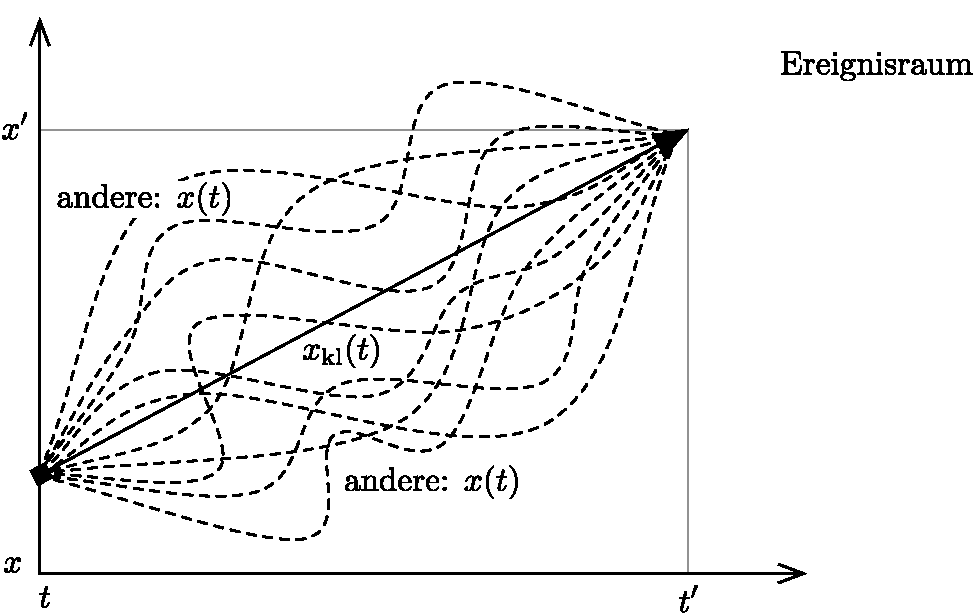
\includegraphics[scale=.75]{Figs/Pfade}
\end{figure}\vspace{-4ex}

Die Pfadintegralformulierung und ihr Bezug zur bereits wohl bekannten Formulierung der Quantenmechanik lässt sich  besser Verstehen, wenn wir uns das {\bf Doppelspaltexperiment} noch einmal vergegenwärtigen. Dort ist die Wahrscheinlichkeit das Teilchen im Abstand $d_i$ vom Spalt $i\in\{1,2\}$ zu finden durch das Betragsquadrat von $\psi_i\propto\e^{\I\;k\,d_i}$ gegeben, sofern nur ein Spalt offen ist und sofern beide Spalte offen sind durch das Betragsquadrat von $\psi_1+\psi_2$. Dass sich die Wahrscheinlichkeiten auf diese eigenartige Weise aufsummieren, ist dabei eine experimentelle Beobachtung. Wir können uns nun das Experiment verallgemeinert vorstellen für unendlich viele Spalte. Die Wahrscheinlichkeitsamplitude ist dann durch das Integral über die Einzelamplituden gegeben. Die Form der Einzelamplituden können wir uns erschließen, wenn wir uns an die Herleitung der Wellenmechanik in Analogie zur Eikonalgleichung erinnern, in der die Amplituden gegeben sind durch Wellen konstanter Wirkung $\psi=\e^{\;\I/\hbar\cdot S_0}$, so dass für $\hbar\to0$ die Schrödingergleichung in die Hamilton-Jacobi-Gleichung übergeht. Damit sind wir bis auf den Vorfaktor wieder bei der Definition des Propagators. 

Es wird nun auch der Übergang zur klassischen Mechanik leichter deutlich, welche sich also für $S/\hbar\to\infty$ ergeben sollte. Dies lässt sich dadurch erklären, dass in diesem Fall der Phasenfaktor stark oszilliert und somit im Mittel nicht zum Integral beiträgt. Nur der klassische Pfad $x_{\text{kl}}$, für den nach dem Hamiltonschen Prinzip die Wirkung ja stationär $\delta S=0$ wird trägt dann noch zur Zeitentwicklung bei. 

Es ist außerdem anzumerken, dass die Pfadintegralformulierung insbesondere zwei wichtige Vorteile in der Anwendung hat: 
\begin{itemize1}
	\item Zum einen bietet sich die Pfadintegralformulierung durch die Formulierung mittels Integralen für numerische Berechnungen an und lässt sich einfacher approximieren. 
	\item Zum anderen vereinfacht sie die Quantisierung von {\bf Eichtheorien}, da im Gegensatz zur Operatorformulierung die Zeitvariable nicht besonders behandelt werden muss, was in relativistischen Formulierungen, in denen Kovarianz erfüllt sein muss, gewisse Schwierigkeiten hervorruft, die im Pfadintegralformalismus hingegen nicht auftreten. Mehr dazu im nächsten Abschnitt. 
\end{itemize1}


\paragraph{Tunneln aus metastabilem Zustand}

Wir wollen im folgenden als Beispielhafte Anwendung des Pfadintegralformalismus einen eindimensionalen Tunnelprozess in $x$-Richtung zwischen den Punkten $0$ und $a$ im Potential $V(x)$ betrachten. Der klassische Pfad stationärer Wirkung der Lagrangefunktion $\mathcal{L}=T(\dot{x})-V(x)=m/2\cdot\dot{x}^2-V(x)$ kann in diesem Fall für imaginäre Zeiten: $t\to \I\tau$ einfach bestimmt werden. Die Bewegungsgleichung $\mathrm{d}/\mathrm{d}t\;\dell_{\dot{x}}\,\mathcal{L}=-\dell_x\,\mathcal{L}$ kann dann in Abhängigkeit von $\tau$ geschrieben werden als: 
\begin{eqnarray*}
	m\cdot\dell_t^2\; x = -\dell_x\; V(x) &\quad\overset{t\to \I\tau}{\Rightarrow}\quad& m\cdot \dell_{\tau}^2\; x = \dell_x\; V(x) 
\end{eqnarray*}
Dies entspricht der Bewegung im Potential mit umgedrehten Vorzeichen $V(x)\to-V(x)$, also $\mathcal{L}=T(\dell_{\tau}x)+V(x)$. Da in dem System Energieerhaltung $\dell_{\tau} \ham = 0$ gilt, können wir ohne Beschränkung der Allgemeinheit $\ham=T-V=E=:0$ setzen, so dass sich $m/2\cdot(\mathrm{d}x/\mathrm{d}\tau)^2 = V(x)$ ergibt. Damit folgt für die Wirkung entlang des klassischen Pfads $S\big(x_{\text{kl}}(t),0,\tau\big)$: 
\begin{eqnarray*}
	-\I\cdot S\big(x_{\text{kl}},0,t\big) &=& \int_0^{\tau}\mathrm{d}\tau'\!\!\!\!\!\!\!\!\!\!\!\!\!\!\!\!\!\!\!\!\!\!\!\!\!\underbrace{\frac{m}{2}\cdot\Big(\frac{\mathrm{d}x}{\mathrm{d}\tau}\Big)^2+V(x)}_{\qquad\quad\qquad=\;m(\mathrm{d}x/\mathrm{d}\tau)^2\;=\;m\;\mathrm{d}x/\mathrm{d}\tau\cdot\sqrt{2V(x)/m}}\!\!\!\!\!\!\!\!\!\!\!\!\!\!\!\!\!\!\!\!\!\!\!\!\! = \int_0^{\tau} \mathrm{d}\tau'\;\frac{\mathrm{d}x}{\mathrm{d}\tau'}\; \sqrt{2mV(x)} = \int_0^a\mathrm{d}x\; \sqrt{2m V(x)}
\end{eqnarray*}
Der führende Ausdruck im Propagator ist damit der Näherungsausdruck für die Tunnelamplitude, wie er sich aus der Wentzel–Kramers–Brillouin ({\bf WKB}) Methode ergibt: 
\begin{eqnarray*}
	K(0,0,a,t) &\approx& C\cdot\e^{\;\frac{\I}{\hbar}\cdot S(x_{\text{kl}},0,t)}=C\cdot\e^{\;\frac{1}{\hbar}\cdot\int_0^a\mathrm{d}x\;\sqrt{2mV(x)}}
\end{eqnarray*}


\paragraph{Statistische Mechanik eines Teilchens}
Die Zustandsumme $Z$ eines Teilchens im Potential $V(x)$ ist in der statistischen Mechanik gegeben durch: 
\begin{eqnarray*}
	Z &=& \Sp\big(\e^{-\beta\hat{\ham}}\,\big) = \int \mathrm{d}x\; \bracket{x}{\e^{-\beta\hat{\ham}}}{x} \qquad \text{mit: } \beta=\frac{1}{k_BT}
\end{eqnarray*}
Sie spielt eine wichtige Rolle, da sie in der Maxwell-Boltzmann-Verteilung auftaucht, welche die Wahrscheinlichkeit $p_{E_n}$ beschreibt, das das System in einem bestimmten Zustand der Energie $E_n$ zu finden: $p_{E_n}=1/Z\cdot\e^{-\beta E_n}$. 

Wir sehen, dass die Zustandssumme dabei grade dem Propagator $K(x,0,x,t)=\bracket{x}{\e^{-\I/\hbar\cdot \hat{\ham}t}}{x}$ entspricht, wenn wir die imaginäre Zeit $t\to \I\hbar \beta$ verwenden. Es ergbit sich dann folgender Ausdruck für die Zustandssumme als Pfadintegral: 
\begin{eqnarray*}
	Z \;= \int\mathrm{d}x\;\bracket{x}{\e^{-\beta\hat{\ham}}}{x} \;= \int \mathrm{d}x\!\!\!\!\underset{x(0)=x,\;x(\beta)=x}{\int \mathscr{D}x} \e^{-\frac{1}{\hbar}\int_0^{\hbar\beta}\mathrm{d}\tau\; \frac{m}{2}\left(\!\frac{\mathrm{d}x}{\mathrm{d}\tau}\!\right)^2+V(x)}
\end{eqnarray*}
Das Pfadintegral berücksichtigt dabei die quantenmechanischen Fluktuationen, welche proportional zu $\Delta x$  sind. Es gilt: 
\begin{eqnarray*}
	\Delta x \propto \sqrt{\frac{2\pi \hbar^2}{m k_B T}} =: \lambda_{\text{therm}}
\end{eqnarray*}
Wobei $\lambda_{\text{therm}}$ als thermodynamische De-Broglie-Wellenlänge bezeichnet wird. Im klassischen Grenzfall, wenn sich $V(x)$ auf der Scala von $\lambda_{\text{therm}}$ nur wenig ändert, können wir den Propagator dann auf den Propagator eines freien Teilchens $K_{\text{frei}}$ reduzieren und es ergibt sich die klassische Zustandssumme mit dem bekannten Vorfaktor: 
\begin{eqnarray*}
	Z \;= \int\mathrm{d}x\;\bracket{x}{\e^{-\beta\hat{\ham}}}{x} \;\approx\; \int \mathrm{d}x\;\e^{-\beta V(x)}\cdot\!\!\!\!\!\!\!\!\! \underbrace{\underset{x(0)=x,\;x(\beta)=x}{\int \mathscr{D}x} \e^{-\frac{m}{2\hbar}\int_0^{\hbar\beta}\mathrm{d}\tau\; \left(\!\frac{\mathrm{d}x}{\mathrm{d}\tau}\!\right)^2}}_{=\; K_{\text{frei}}(x,-\I\hbar\beta,x,0)\;=\;\sqrt{\frac{mk_BT}{2\pi\hbar^2}}} &=& \int \mathrm{d}x\;\;\frac{\e^{-\beta V(x)}}{\lambda_{\text{therm}}}
\end{eqnarray*}




\subsubsection{Eichtransformationen in der Quantenmechanik}

Als Eichtransformation bezeichnet man eine Transformation sogenannter Eichfelder, beispielsweise die elektromagnetischen Potentiale, unter der die Dynamik eines Systems invariant bleibt. Man unterscheidet dabei zwischen {\bf globalen Eichtransformationen}, welche die Eichfelder an allen Orten um einen Faktor verschiebt, Beispiel hierfür sind Nullpunktsverschiebungen, und {\bf lokalen Eichtransformationen}, welche die Eichfelder um eine ortsabhängige Funktion verschiebt. Wenn die Dynamik einer Feldtheorie aus einer lokal eichinvarianten, also unter Eichtransformationen unveränderten, Wirkung folgt, so wird die physikalsiche Theorie auch als {\bf Eichtheorie} bezeichnet und man spricht davon, dass die Theorie einer lokalen Eichsymmetrie genügt. 

Wir haben gesehen, dass sich die Quantenmechanik durch den Pfadintegralformalismus aus der Wirkung ableiten lässt und wir erinnern uns, dass die Wirkung für elektromagnetische Felder im klassischen Fall eichinvariant war. Die Quantenmechanik sollte also auch eine Eichtheorie sein. Dies wollen wir im folgenden auch explizit in der kanonischen Formulierung der Quantenmechanik zeigen. 

Dazu erinnern wir uns zunächst, dass der Hamiltonoperator $\hat{\ham}$ eines Teilchens in einem elektromagnetischen Feld mit skalarem Potential $\hat{\phi}(\hat{\vec{r}},t)$ und Vektorpotential $\hat{\vec{A}}(\hat{\vec{r}},t)$ gegeben war durch:
\begin{eqnarray*}
	\hat{\ham}(\hat{\vec{r}},\hat{\vec{p}},t) &=& \frac{1}{2m}\cdot \big(\hat{\vec{p}}-q\cdot\hat{\vec{A}}(\hat{\vec{r}},t)\big)^2 + q\cdot\hat{\phi}(\hat{\vec{r}},t)
\end{eqnarray*}
Wir definieren nun den {\bf Geschwindigkeitsoperator} $\hat{\vec{v}}=\mathrm{d}/\mathrm{d}t\;\hat{\vec{r}}$, dessen explizite Darstellung sich aus der Heisenberg Gleichung (\ref{HG}) ergibt zu: 
\begin{eqnarray*}
	\hat{\vec{v}} &=& \frac{\mathrm{d}}{\mathrm{d}t}\;\hat{\vec{r}} = - \frac{\I}{\hbar} [\hat{\vec{r}},\hat{\ham}] = -\frac{\I}{2m\hbar}\Big[\hat{\vec{r}}\;,\;\hat{\vec{p}}\,^2-q\cdot\hat{\vec{p}}\hat{\vec{A}}- q\cdot\hat{\vec{A}}\hat{\vec{p}}\,\Big] = -\frac{1}{m}\cdot(\hat{\vec{p}}-q\cdot \hat{\vec{A}}\,)
\end{eqnarray*} 
Dabei vertauschen die Komponenten des Geschwindigkeitsoperators $\hat{v}_i$ mit $i\in\{x,y,z\}$ nicht untereinander und es lässt sich mit Hilfe von $\hat{\vec{B}}=\rot\hat{\vec{A}}$ folgende Relation finden: 
\begin{eqnarray*}
	[\hat{v}_i,\hat{v}_j] &=& -\frac{q}{m^2}\cdot \underset{\;}{\Big(} [\hat{p}_i,\hat{A}_j] + [\hat{A}_i,\hat{p}_j] \Big) = \frac{\I\hbar q}{m^2}\cdot(\partial_i\hat{A}_j-\partial_j\hat{A}_i) = \frac{\I\hbar q}{m^2}\cdot \varepsilon_{ijk}\hat{B}_k
	\\
	&&\Rightarrow\quad \hat{\vec{v}}\times\hat{\vec{v}} = \frac{\I q\hbar}{m^2}\cdot \hat{\vec{B}}
\end{eqnarray*} 
Mit Hilfe des Geschwindigkeitsoperators $\hat{\vec{v}}(\hat{\vec{r}},\hat{\vec{p}},t)$ können wir den Hamiltonoperator $\hat{\ham}$ nun schreiben wie folgt:
\begin{eqnarray*}
	\hat{\ham}(\hat{\vec{r}},\hat{\vec{p}},t) &=& \frac{m}2\cdot\hat{\vec{v}}(\hat{\vec{r}},\hat{\vec{p}},t)^2 + q\cdot\hat{\phi}(\hat{\vec{r}},t) 
\end{eqnarray*}
Die {\bf Wahrscheinlichkeitsstromdichte} $\vec{j}$ ergibt sich nun mit dem verallgemeinerten Impulsoperator im Ortsraum $\hat{\vec{p}}\to m\cdot\hat{\vec{v}}=-\I\hbar\cdot\vec{\nabla}-q\cdot\vec{A}$ zu: 
\begin{eqnarray*}
	\vec{j} &=& \frac{1}{2m} \cdot\Big(\psi^*(-\I\hbar\cdot\vec{\nabla}-q\cdot\vec{A}\,)\;\psi - \psi\;(-\I\hbar\cdot\vec{\nabla}-q\cdot\vec{A}\,)\;\psi^*\underset{\;}{\Big)}
	\\
	&=& -\frac{\I\hbar}{2 m}\cdot\big(\psi^*(\vec{\nabla}\psi)-\psi\;(\vec{\nabla}\psi^*)\big) - \frac{q}{m} \cdot |\psi|^2 \vec{A}
\end{eqnarray*}
Und erfüllt wie man leicht sieht weiterhin die Kontinuitätsgleichung: $\partial_t |\psi|^2+\vec{\nabla}\vec{j}=0$.

Wir wollen nun das Verhalten unter den folgenden aus der Elektrodynamik bekannten lokalen Eichtransformationen im Ortsraum an den Potentialen betrachten, welche zwar den Hamiltonoperator verändern werden, die elektromagnetischen $\vec{E}$- und $\vec{B}$-Felder jedoch unverändert lässt:
\begin{alignat*}{4}
	\vec{A}(\vec{r},t) &\qquad\to\qquad& \vec{A}\,'(\vec{r},t) &\;=\;\;& \vec{A}(\vec{r},t) + \vec{\nabla}\Lambda(\vec{r},t)
	\\
	\phi(\vec{r},t) &\qquad\to\qquad& \phi'(\vec{r},t) &\;=\;\;& \phi(\vec{r},t) - \dell_t\Lambda(\vec{r},t)
\end{alignat*}
Wir wollen nun zeigen, dass sich die Eichinavrianz der Schrödingergleichung unter dieser Eichtransformation durch eine lokale Phasentransformation der Wellenfunktion $\psi(\vec{r},t)$ mit dem unitären Operator $U(\vec{r},t)$ erreichen lässt: 
\begin{alignat*}{4}
	\psi(\vec{r},t) &\qquad\to\qquad& \psi'(\vec r,t) &\;=\;\;& \underbrace{\e^{\;\frac{\I}{\hbar}q\cdot \Lambda(\vec{r},t)}}_{=\;U(\vec{r},t)} \psi(\vec{r},t) = U(\vec{r},t)\cdot\psi(\vec{r},t)
\end{alignat*}
Wir wollen nun die Wirkung der Eichtransformation auf die Operatoren $\hat{\vec{r}}$, $\hat{\vec{p}}$ und $\hat{\vec{v}}$ untersuchen. Dazu untersuchen wir die Erwartungswerte der Operatoren $\hat{\vec{o}}\,$: 
\begin{eqnarray*}
	\EW{\hat{\vec{o}}\,}'=\bracket{\psi'}{\hat{\vec{o}}\,}{\psi'}=\bracket{\psi}{\hat{U}^{\dagger}\hat{\vec{o}}\,\hat{U}}{\psi}=\EW{\hat{U}^{\dagger}\hat{\vec{o}}\,\hat{U}} &\quad\Rightarrow\quad& \EW{\hat{\vec{o}}\,}'=\EW{\hat{\vec{o}}\,}\;\Leftrightarrow\;[\hat{\vec{o}},\hat{U}]=0
\end{eqnarray*}
Ein Operator ist also invariant unter der Eichtransformation wenn er mit dem unitären Operator $\hat{U}$ der Phasentransformation vertauscht. Für die Operatoren $\hat{\vec{r}}$ und $\hat{\vec{p}}$ ergibt sich somit bei der Untersuchung im Ortsraum folgendes: 
\begin{eqnarray*}
	\big[\vec{r},U(\vec{r},t)\big] &=& 0  
	\\
	\big[\hat{\vec{p}},U(\vec{r},t)\big] &=& \big[-\I\hbar\cdot\vec{\nabla},U(\vec{r},t)\big] = -\I\hbar\cdot\big(\vec{\nabla}U(\vec{r},t)\big) = q\cdot\big(\vec{\nabla}\Lambda(\vec{r},t)\big)\cdot U(\vec{r},t) \neq 0
\end{eqnarray*}
Der Impulsoperator ist also nicht eichinvariant, der Ortsoperator hingegen schon. Wir wollen nun noch den Geschwindigkeitsoperator $\hat{\vec{v}}$ betrachten, für den wir folgende Beziehung finden können: 
\begin{eqnarray*}
	m\cdot U^{\dagger}\hat{\vec{v}}\,U &=& U^{\dagger}(\hat{\vec{p}}-q\cdot\vec{A}\,)U = U^{\dagger}(U\hat{\vec{p}}+\!\!\!\!\!\!\!\underbrace{[\,\hat{\vec{p}},U]}_{\quad=\;q\cdot U (\vec{\nabla}\Lambda)}\!\!\!\!\!\!)-q\cdot U^{\dagger}U\vec{A} = \hat{\vec{p}} -q\cdot(\vec{\nabla}\Lambda+\vec{A}) 
	\\
	&=& \hat{\vec{p}}-q\cdot\vec{A}\,'= m\cdot\hat{\vec{v}}\,' \qquad\qquad\qquad\qquad\qquad\qquad\Rightarrow\quad\EW{\hat{\vec{v}}\,}=\EW{\hat{\vec{v}}\,'}'
\end{eqnarray*}
Die Schrödingergleichung $\I\hbar\cdot\dell_t \psi=\hat{\ham}\psi$ ist somit invariant, wenn wir den Hamiltonoperator transformieren $\hat{\ham}\to\hat{\ham}'$ zu:
\begin{eqnarray*}
	\hat{\ham}' &=& U\hat{\ham}U^{\dagger}+\I\hbar\cdot U^{\dagger}\partial_t U = \frac{m}{2}\cdot \hat{\vec{v}}\,'\,\!^2+q\cdot\hat{\phi}-q\cdot\dell_t\Lambda = \frac{m}{2}\cdot \hat{\vec{v}}\,'\,\!^2+q\cdot\hat{\phi}' \quad\Rightarrow\quad \I\hbar\dell_t\psi'=\hat{\ham}'\psi'
\end{eqnarray*}
Wir können somit als Fazit festhalten, dass die Quantenmechanik tatsächlich invariant ist unter den aus der Elektrodynamik bekannten Eichtransformationen und sich die Zustände um einen Phasenfaktor transformieren $\psi' =\psi\cdot\e^{\;\I/\hbar\cdot q\Lambda(\vec{r},t)}$, welcher keinen Einfluss auf die physikalischen Ergebnisse hat. 


\subsubsection{Der Aharonov-Bohm-Effekt}

Wir wollen uns im folgenden noch mit einem interessanten Effekt Beschäftigen, welcher aus der Struktur der quantenmechanischen Theorie folgt und ein neues Licht auf die Bedeutung der Potentiale von Feldern wirft, welche in der klassischen Mechanik ja keine physikalische Existenz haben, sondern nur mathematische Hilfskonstrukte sind. 

Dazu stellen wir uns ein Doppelspaltexperiment vor und fügen zwischen den beiden Spalten eine Box ein, in der ein Magnetfeld $\vec{B}$ herrscht welches allerdings vom Außenraum komplett abgeschirmt ist: $\vec{B}(\vec{r}\notin\text{Box}) = 0$. Das Vektorpotential $\vec{A}$ erstrecke sich jedoch auf den gesamten Raum. Die folgende Abbildung soll diesen Aufbau veranschaulichen: 
\vspace{-2ex}\begin{figure}[!h]\centering
	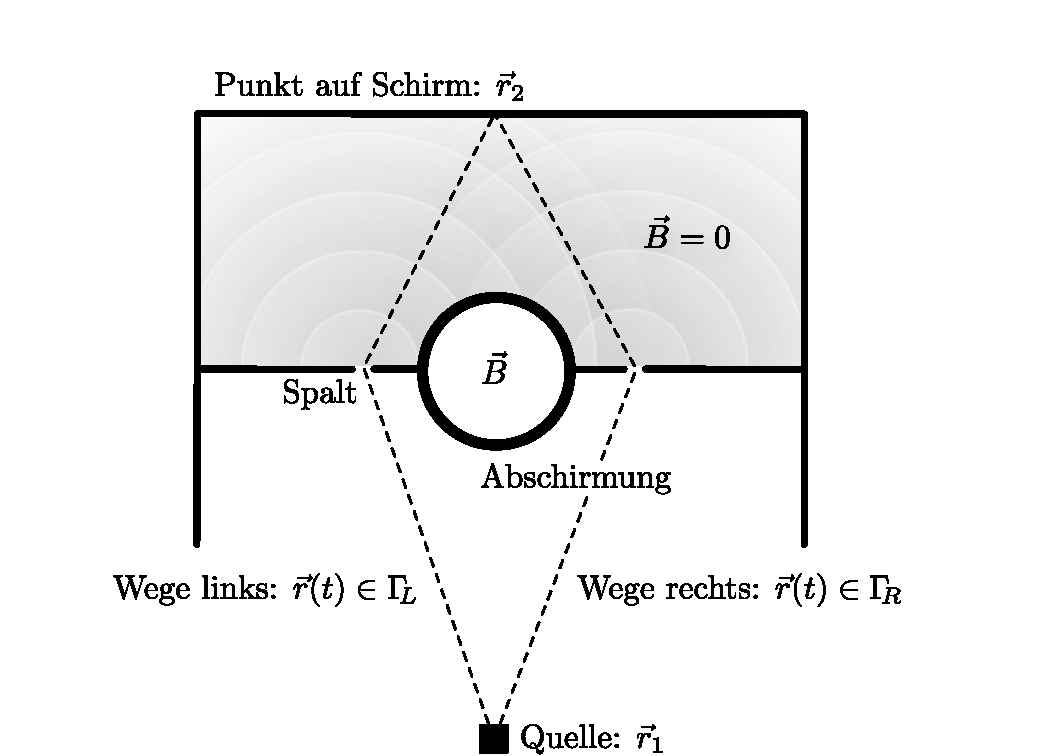
\includegraphics[scale=0.75]{Figs/DoppelspaltB}
\end{figure}

Wir wollen nun untersuchen, ob die Präsenz des Feldes $\vec{B}=\rot\vec{A}$ einen Einfluss auf unsere Messung hat. Dazu definieren wir zunächst den magnetischen Fluss $\phi_B(A)$ durch eine Fläche $A$, welcher nach dem Satz von Stokes für ein Magnetfeld durch die Fläche $A$ mit Normalenvektor $\vec{n}_A$ und Rand $\dell A$ gegeben ist durch:
\begin{eqnarray*}
	\phi_B(A) &=& \int_A\mathrm{d}\vec{A}\;\vec{B} = \int_A\mathrm{d}\vec{n}_A\; \vec{\nabla}\times\vec{A} = \oint_{\dell A}\mathrm{d}\vec{s}\; \vec{A} 
\end{eqnarray*}
Um die Bedingung zu erfüllen, dass das $\vec{B}$-Feld im Außenraum verschwindet, können wir das Vektorpotential $\vec{A}$ beispielsweise als reines Gradientenfeld definieren: $\vec{A}(\vec{r})=\vec{\nabla}\Lambda(\vec{r})$. Wenn wir beispielsweise ein Magnetfeld $\vec{B}$ betrachten, welches einen Zylinder mit Radius $R$ in $z$-Richtung durchdringt, so ergibt sich der gesamte magnetische Fluss durch die Fläche $\pi R^2$ zu $\phi_B=\pi R^2\cdot B$. Ein mögliches $\Lambda$ um das zugehörige Vektorpotential $\vec{A}$ als Gradientenfeld zu definieren wäre dann in Zylinderkoordinaten $\vec{r}=\varphi\cdot\vec{e}_{\varphi}+\rho\cdot\vec{e}_{\rho}+z\cdot\vec{e}_{z}$ beispielsweise durch $\Lambda=\phi_B/1\pi\cdot\varphi$ gegeben. Das Vektorpotential ergibt sich dann zu $\vec{A}=\phi_B/2\pi\rho\cdot \vec{e}_{\varphi}$. Die mögliche Wahl des Vektorpotentials als reines Gradientenfeld und nicht einfach als 0 ist dabei eine direkte Folge der Eichinvarianz, wegen der das verschwindende magnetische Feld $\vec{B}=0$ das Vektorpotential eben nicht eindeutig, sondern nur bis auf eine Eichtransformation bestimmt. 

Wir wollen nun betrachten, was mit dem Interferenzbild passiert. Dabei lässt sich aus den Überlegungen im vorigen Abschnitt einsehen, dass sich durch die Eichtransformation ein Phasenfaktor ergibt, der potentiell Einfluss auf die Wahrscheinlichkeitsamplitude haben kann, da sich diese ja als Betragsquadrat aus der Summe der Wellenfunktion für den Weg durch beide Spalte ergibt. Wenn zwischen den beiden Wegen also durch das Einschalten des Potentials ein Phasenunterschied vorliegt, so verändert sich das Interferenzmuster. Wir wollen dies im folgenden anhand des Propagators näher untersuchen. 

Wenn wir einen Propagator von der Quelle am Ort $\vec{r}_1=\vec{r}(t_1)$ zu einem Punkt auf dem Schirm bei $\vec{r}_2=\vec{r}(t_2)$ betrachte, so ergibt sich der Propagator zu:
\begin{eqnarray*}
	K(\vec{r}_1,t_1,\vec{r}_2,t_2) &=& \!\!\!\!\!\!\!\!\!\!\!\underset{\vec{r}(t_2)=\vec{r}_2,\;\vec{r}(t_1)=\vec{r}_1}{\int\mathscr{D}\vec{r}} \!\!\!\! \e^{\;\frac{\I}{\hbar} S(\vec{r}(t),t_1,t_2)} 
\end{eqnarray*}
Die Wirkung ergibt sich dabei für ein Teilchen im Vektorpotential $\vec{A}$ zu: 
\begin{eqnarray*}
	S\big(\vec{r}(t),t_1,t_2\big) = \underbrace{\int_{t_1}^{t_2}\!\!\!\!\mathrm{d}t\; \Big(\frac{m}{2}\cdot \dot{\vec{r}}\,^2 - V(\vec{r})\Big)}_{=\;S(\vec{r}(t),t_1,t_2)\left|_{\vec{A}=0}\right.} + \;q\cdot\!\!\!\!\!\!\!\!\!\!\!\!\!\underbrace{\int_{t_1}^{t_2}\!\!\!\!\mathrm{d}t\;\dot{\vec{r}}\vec{A}}_{\qquad =\;\int_{\gamma(\vec{r}_1,\vec{r}_2)}\mathrm{d}\vec{s}\;\vec{A}}\!\!\!\!\!\!\!\!\! = S\big(\vec{r}(t),t_1,t_2\big)\big|_{\vec{A}=0}+q\cdot\!\!\underbrace{\big(\Lambda(\vec{r}_2)-\Lambda(\vec{r}1)\big)}_{=\;\phi_B(\vec{r}(t),\vec{r}_1,\vec{r}_2)}
\end{eqnarray*}
Dabei ist $\phi_B\big(\vec{r}(t),\vec{r}_1,\vec{r}_2\big)$ magnetische Fluss durch die vom Weg $\vec{r}(t)$ zwischen $\vec{r}_1$ und $\vec{r}_2$ eingeschlossene Fläche. Wir wollen nun die Gesamtheit der Wege aufteilen in die Menge aller Wege durch den linken Spalt $\Gamma_{\!\!L}$ und die Menge aller Wege durch den rechten Spalt $\Gamma_{\!\!R}$. Dabei unterscheidet sich die Wirkung in diesen beiden Teilmengen strukturell nicht im Teil $S\big(\vec{r}(t),t_1,t_2\big)\big|_{\vec{A}=0}$. Wir können dann das Pfadintegral aufteilen in zwei Teile und folgendes schreiben: 
\begin{eqnarray*}
	&&K(\vec{r}_1,t_1,\vec{r}_2,t_2) \quad=\quad \int_{\vec{r}_1}^{\vec{r}_2}\!\!\!\!\!\mathscr{D}\vec{r}\; \e^{\;\frac{\I}{\hbar} S(\vec{r}(t),t_1,t_2)} \;\Big|_{\vec{r}(t)\,\in\,\Gamma_{\!L}} \!\!\!+ \int_{\vec{r}_1}^{\vec{r}_2}\!\!\!\!\!\mathscr{D}\vec{r}\; \e^{\;\frac{\I}{\hbar} S(\vec{r}(t),t_1,t_2)} \;\Big|_{\vec{r}(t)\,\in\,\Gamma_{\!R}} 
	\\
	&&\quad = \int_{\vec{r}_1}^{\vec{r}_2}\!\!\!\!\!\mathscr{D}\vec{r}\; \e^{\;\frac{\I}{\hbar} \left(S(\vec{r}(t),t_1,t_2)\left|_{\vec{A}=0}\right.+q\phi_B(\vec{r}(t),\vec{r}_1,\vec{r}_2)\right)} \;\Big|_{\vec{r}(t)\,\in\,\Gamma_{\!L}} \!\!\!+ \int_{\vec{r}_1}^{\vec{r}_2}\!\!\!\!\!\mathscr{D}\vec{r}\; \e^{\;\frac{\I}{\hbar} \left(S(\vec{r}(t),t_1,t_2)\left|_{\vec{A}=0}\right.+q\phi_B(\vec{r}(t),\vec{r}_1,\vec{r}_2)\right)} \;\Big|_{\vec{r}(t)\,\in\,\Gamma_{\!R}}
	\\
	&&\quad = \int_{\vec{r}_1}^{\vec{r}_2}\!\!\!\!\!\mathscr{D}\vec{r}\; \e^{\;\frac{\I}{\hbar} S(\vec{r}(t),t_1,t_2)\left|_{\vec{A}=0}\right.} \cdot \underbrace{\e^{\;\frac{\I}{\hbar}q\cdot\left(\phi_B(\vec{r}(t),\vec{r}_1,\vec{r}_2)\left|_{\vec{r}(t)\in\,\Gamma_{\!L}}\right.-\phi_B(\vec{r}(t),\vec{r}_2,\vec{r}_1)\left|_{\vec{r}(t)\in\,\Gamma_{\!R}}\right.\right)}}_{=:\;\e^{\I/\hbar\cdot q\cdot\Delta_{LR}\,\phi_{B}}}
\end{eqnarray*}
Der Phasenunterschied zwischen den Wegen auf der rechten Seite $\gamma\in\Gamma_{\!\!R}$ und der linken Seite $\gamma\in\Gamma_{\!\!L}$ ergibt sich dabei zu: 
\begin{eqnarray*}
	\quad\Delta_{LR}\,\phi_{B} = \frac{q}{\hbar}\cdot \bigg(\int_{\gamma(\vec{r}_1,\vec{r}_2)\in\Gamma_{\!L}}\!\!\!\!\!\!\!\!\!\!\!\!\!\!\!\!\!\!\mathrm{d}\vec{s}\;\vec{A}\;\;-\int_{\gamma(\vec{r}_2,\vec{r}_1)\in\Gamma_{\!R}}\!\!\!\!\!\!\!\!\!\!\!\!\!\!\!\!\!\!\mathrm{d}\vec{s}\;\vec{A}\quad\bigg) = \frac{q}{\hbar}\oint_{\gamma\in\,\Gamma_{\!L}\times\Gamma_{\!R}}\!\!\!\!\!\!\!\!\!\!\!\!\!\!\!\mathrm{d}\vec{s}\; \vec{A} = 2\pi\cdot\!\!\!\!\!\underbrace{\frac{q}{2\pi\hbar}}_{\quad=\;1/\Phi_0}\!\!\!\!\! \cdot\phi_B(A_{\gamma}) = 2\pi\cdot\frac{\phi_B(A_{\gamma})}{\Phi_0} 
\end{eqnarray*}
Dabei wird $\Phi_0$ als Flussquantum bezeichnet. Wir sehen also, dass die Phase nur davon abhängt, ob die möglichen Wege den Fluss eines magnetischen Feldes durch eine Fläche einschließen, nicht ob sie durch diesen führen. Und wir sehen, dass die Postition der Interferenzmaxima durch die Existenz dieses magnetischen Flusses abhängt, weil sie den Propagator signifikant beeinflusst. 

Wir können also festhalten, dass in der Quantenmechanik nicht nur Kraftfelder Einfluss auf die Dynamik eines Systems nehmen können, sondern auch ohne den direkten Einfluss eines Lorentzkraft auf ein geladenenes Teilchen, dessen Bewegung beeinflusst werden kann. Dies ist direkt dadurch bedingt, dass in der Quantenmechanik die Dynamik nicht furch einen determinierten Weg des Teilchens beschrieben wird, sondern alle möglichen Wege die Dynamik des Teilchens beeinflussen und somit ein durch diese Möglichen Wege eingeschlossener Fluss einen Einfluss haben kann. 

Die Interpretation der Kraftfelder stellt einen bedeutenden Unterschied der Quantenmechanik zur klassischen Mechanik da. Es gibt generell zwei Möglichkeiten die Bedeutung von Feldern in der Quantenmechanik zu interpretieren: 
\begin{itemize1}
\item Entweder in der Quantenmechanik sind die elektromagnetischen Potentiale $\vec{A}$ und $\phi$ die Grundlegenden physikalische Größen, anstelle der Felder $\vec{E}$ und $\vec{B}$. Jedoch gilt für sie weiterhin die Eichfreiheit. 
\item Oder die Felder $\vec{E}$ und $\vec{B}$ werden weiterhin als die Grundlegenden physikalische Größen betrachtet, aber es wird akzeptiert, dass sie auf nicht-lokale Weise wechselwirken können. Es müsste also die {\bf Lokalität} der Theorie aufgegeben werden. 
\end{itemize1}

%\end{document} \newpage
\thispagestyle{plain} %\documentclass[a4paper,12pt,final,twoside]{scrartcl}
\setcounter{secnumdepth}{3}
\setcounter{tocdepth}{5}

\usepackage[utf8]{inputenc}
\usepackage[T1]{fontenc}
\linespread{1.4}
\usepackage{dsfont}
\usepackage{amsfonts}
\usepackage{amsmath}
\usepackage{amssymb}
\usepackage{amsthm}
\usepackage{mathtools}
\usepackage{mathbbol}
\usepackage{amsmath1}
\usepackage[ngerman]{babel}
\usepackage{bibgerm}
\usepackage[pdftex]{graphicx}
%\usepackage{mathpazo}
\usepackage{floatflt}
%%\usepackage{epsfig}
\usepackage{wrapfig}
\usepackage{graphicx}
\usepackage{tabularx}
\usepackage{caption} 
\usepackage{multicol} 
\usepackage{mathrsfs}
%\usepackage{pspicture}
%\usepackage{eepic}
%\usepackage{epic}
%\usepackage{trfsigns}

%\usepackage[ansinew]{inputenc}
\usepackage{longtable,array,dcolumn}
%\usepackage{ngerman}
\usepackage{epic}
\usepackage{rotate}
\usepackage{graphpap}
\usepackage{amssymb}
\usepackage[squaren]{SIunits}
\usepackage{curves}
\usepackage{float}
\usepackage{array}
\usepackage{enumerate}
\usepackage{marvosym}
\usepackage{slashed}%für feynmanslsash
\usepackage[breaklinks,pdfborder={0 0 0}]{hyperref}
\usepackage{ulem}	%angeblich funktioniert dann
\let\underbar\uline	%underbar in math auch bei greek letters
\usepackage{multirow}
%\usepackage{multicolumn}
\usepackage{enumitem}


\setlength{\parskip}{12pt}
\setlength{\parindent}{0mm}
%\newcommand{\grad}{\ensuremath{^{\circ}}
%\renewcommand{\figurename}{Abb.}		% mit usepackage caption2
%\renewcommand{\captionfont}{\small \itshape}	% mit usepackage caption2
%\setkomafont{caption}{\small \itshape}		%sollte mit caption im userpackage funktionieren
%\setkomafont{captionlabel}{\small , \itshape}	%sollte mit caption im userpackage funktionieren
\captionsetup{font = {small, sf}} %mit it anstelle von sf gibts kusiv

\date{2009-20-10}
\newcommand{\kreis}[1]{
 \qbezier(-#1,0)(-#1,#1)(0,#1)
  \qbezier(0,#1)(#1,#1)(#1,0)
  \qbezier(#1,0)(#1,-#1)(0,-#1)
  \qbezier(0,-#1)(-#1,-#1)(-#1,0)}
\newcommand{\s}{\ \big| \ }
\newcommand{\lo}{\left <}
\newcommand{\ro}{\ri >}
\newcommand{\g}{&=&}

\newcommand{\ham}{\mathcal H}
\newcommand{\hil}{\mathscr H}
\newcommand{\fok}{\mathscr F}
\newcommand{\wh}{\widehat}
%\newcommand{\left}{\left}
\newcommand{\ri}{\right}
\newcommand{\Sp}{\text{Sp}}
\newcommand{\babsatz}{\par \begingroup \leftskip=2cm}
\newcommand{\eabsatz}{\par\endgroup}

\newcommand{\D}{\text{\itshape D}}
\newcommand{\Lr}{\mathcal L }%\textit{L}}
\newcommand{\rot}{\text{rot}}
\newcommand{\divergenz}{\text{div}}
\newcommand{\grad}{\text{grad}}
\newcommand{\grat}{${}^{\circ}$}
%\newcommand{\tanh}{\text{tanh}} already defined

\newcommand{\RM}[1]{\text{\MakeUppercase{\romannumeral #1}}}
\newcommand{\dell}{\partial}
\renewcommand{\div}{\operatorname{div}}
\newcommand{\I}{\dot{\text{\i\!\i}}}
\newcommand{\e}{\mathrm{e}}
\newcommand{\ket}[1]{\mid\!\!\!\,\,{#1}\rangle}
\newcommand{\bra}[1]{\langle{#1}\!\!\!\,\,\mid}
\newcommand{\braket}[2]{\langle{#1}\!\!\!\,\,\mid\!\!\!\,\,{#2}\rangle}
\newcommand{\bracket}[3]{\langle{#1}\!\!\!\,\,\mid\!\!\!\,\,{#2}\!\!\!\,\,\mid\!\!\!\,\,{#3}\rangle}
\newcommand{\1}{\mathds{1}}
\newcommand{\EW}[1]{\langle\!\!\,\,#1\!\!\,\,\rangle}
\newcommand{\arrowbox}[1]{-\!\!\!\!\:\text{(#1)}\!\!\!\;\;\!\!\!\rightarrow}

\newcommand{\ketI}[1]{\ket{#1}_{\!\!\;\text{I}}}
\newcommand{\ketII}[1]{\ket{#1}_{\!\!\;\text{II}}}
\newcommand{\ketIII}[1]{\ket{#1}_{\!\!\;\text{III}}}
\newcommand{\braI}[1]{\,\!_{\text{I}\!\!\;}\bra{#1}}
\newcommand{\braII}[1]{\,\!_{\text{II}\!\!\;}\bra{#1}}
\newcommand{\braketI}[2]{\,_{\text{I}\!\!\;}\braket{#1}{#2}_{\!\!\;\text{I}}\,}
\newcommand{\braketII}[2]{\,_{\text{II}\!\!\;}\braket{#1}{#2}_{\!\!\;\text{II}}\,}
\newcommand{\braketIII}[2]{\,_{\text{III}\!\!\;}\braket{#1}{#2}_{\!\!\;\text{III}}\,}
\newcommand{\bracketI}[3]{\,_{\text{I}\!\!\;}\bracket{#1}{#2}{#3}_{\!\!\;\text{I}}\,}
\newcommand{\bracketII}[3]{\,_{\text{II}\!\!\;}\bracket{#1}{#2}{#3}_{\!\!\;\text{II}}\,}


\newcommand{\up}{\ket{\uparrow}}
\newcommand{\updg}{\bra{\uparrow}}
\newcommand{\down}{\ket{\downarrow}}
\newcommand{\downdg}{\bra{\downarrow}}
\newcommand{\upup}{\ket{\uparrow\uparrow}}
\newcommand{\updown}{\ket{\uparrow\downarrow}}
\newcommand{\downup}{\ket{\downarrow\uparrow}}
\newcommand{\downdown}{\ket{\downarrow\downarrow}}

\newenvironment{itemize1}{\begin{itemize}[leftmargin=5mm,itemsep=-1ex,topsep=-1ex]}{\end{itemize}}

%\usepackage[left=2cm,right=2cm,top=1cm,bottom=1cm,includeheadfoot]{geometry}

\usepackage{fancyhdr}
\pagestyle{fancy}{\fancyhf{}
\fancyhead[LO,RE]{\footnotesize \rightmark}
\fancyfoot[C]{\footnotesize -$\,$\thepage$\;$-}
\renewcommand{\headrulewidth}{0.4pt}
\renewcommand{\footrulewidth}{0pt}}

\fancypagestyle{plain}{\fancyhf{}
\renewcommand{\headrulewidth}{0.4pt}
\fancyfoot[C]{\footnotesize -$\,$\thepage$\,$-}}

\usepackage{titlesec}
\titleformat{\section}[display]{\sffamily\bfseries\Huge\center}{Kapitel \thetitle:}{1ex}{}{}
\newcommand{\kapitel}[2]{$\;$\vspace{-1.5cm} \section[#1]{#2} \rule{17cm}{0.4pt}\vspace{3cm}}
\titleformat{\paragraph}[hang]{\sffamily\bfseries}{\thetitle:}{0ex}{\vspace{-0.15cm}}{\vspace{0.5cm}}

\title{ \vspace{1.5cm}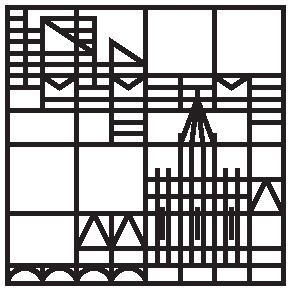
\includegraphics[width=5cm]{logo}
\\ \Large Universität Konstanz  \\ \vspace{4ex} \huge 
Skript zur Vorlesung\\ Höhere Quantentheorie und Elektrodynamik
\\ \vspace{4ex} \Large Prof. Dr. Wolfgang Belzig 
\\ Version vom 30. Juli 2012 \\ \vspace{4.5cm}
\normalsize Ursprünglichen Mitschrift von Birte Heinze im WS 09/10 \\ Ausführliche Überarbeitung von Tobias Lohse im WS 11/12 \vspace{-10cm}}
\author{}
\date{}
%\begin{document}


\subsection{Wahrscheinlichkeitsinterpretation und Messprozess}

Die Quantentheorie stellt gegenüber der klassischen Physik eine sehr Unterschiedliche Beschreibung der physikalischen Vorgänge dar. Nicht nur insofern der mathematische Formalismus sich in gravierenden Punkten von der Formulierung der klassischen Physik unterscheidet, sondern insbesondere auch, was die Bedeutung der Begriffe und die Natur der beschriebenen physikalischen Objekte angeht. 

Insbesondere die Beschreibung des Messprozess stellt dabei einen bedeutenden Unterschied zur klassischen Physik dar. Wir erinnern uns, dass bei der Messung einer Observablen der Zustand in den Eigenzustand zum zugehörigen gemessenen Eigenwert übergeht. Die Messung selbst stellt also eine Zeitentwicklung des Systems dar, welche insbesondere nicht umkehrbar ist, von der Messung abhängt und die nicht deterministische Natur der Quantenmechanik vor Augen führt. 	

Unter {\bf Determinismus} versteht man den Sachverhalt, dass der klassische Zustand, also Ort und Impuls, beliebig genau gemessen werden können. Dies ist in der Quantenmechanik nicht gegeben, da Orts und Impulsoperator keine gemeinsamen Eigenzustände haben und somit nach einer Messung von Impuls oder Ort die Information über die andere Größe verloren geht, und auch mit raffinierten Messmethoden nicht gleichzeitig exakt bestimmt werden kann. Die Zeitentwicklung in der Quantenmechanik wie in der klassischen Mechanik ist hingegen deterministisch im kausalen Sinne. Aus einem bekannten Anfangszustand lässt sich der Endzustand eines bekannten Systems, also wenn wir die Hamiltonfunktion und die Randbedingungen kennen, eindeutig ermitteln. Auch die Zeitentwicklung bei der Messung ist deterministisch, da sich der Endzustand bei bekannter Messung eindeutig ergibt. Allerdings wird beim Messprozess die nicht deterministische Natur des quantenmechanischen Zustands deutlich.  

Wir wollen uns im folgenden mit der Beschreibung des Zustands und der den Übergang zu klassischen Systemen durch sogenannte Dekohärenzen eingehen. Abschließend soll noch erörtert werden, ob die Quantenmechanik mittels verborgener Parameter erklärt werden könnte. 



\subsubsection{Messungen und Projektionspostulat}

Wir wollen noch einmal die Aussage des Projektionspostulats wiederholen: Die Messung einer durch den hermiteschen Operator $\hat{A}$ beschriebenen Observable ergibt immer einen Eigenwert $a_n$ des Operators: $\hat{A}\ket{a_n}=a_n\ket{a_n}$. Nach der Messung eines Eigenwerts $a_n$ befindet sich das System dann im zugehörigen Eigenzustand $\ket{a_n}$. Außerdem besagt die Bronsche Wahrscheinlichkeitsinterpretation, dass die Wahrscheinlichkeit das System im Zustand $\ket{a_n}$ zu finden gegeben ist durch $p_n=|\braket{a_n}{\psi}|^2$. Daraus ergibt sich dann, dass der Erwartungswert $\EW{\hat{A}}$ des Operators $\hat{A}$, also der Mittelwert der Messungen, gegeben ist durch: 
\begin{eqnarray*}
	\EW{\hat{A}} &=& \sum_n p_n\cdot a_n = \sum_n \braket{\psi}{a_n}\braket{a_n}{\psi}\cdot a_n = \bra{\psi}\underbrace{\sum_n a_n\cdot \ket{a_n}\bra{a_n}}_{=\; \hat{A}}\;\psi\rangle = \bracket{\psi}{\hat{A}}{\psi}
\end{eqnarray*}
Um die Aussagen des Projektionspostulats einfacher zu formulieren führen wir den sogenannten {\bf Projektionsoperator} $\hat{P}_a$ definieren. Ein hermetischer Projektionsoperator $\hat{P}^{\dagger}=\hat{P}$ ist dabei ganz allgemein durch die Eigenschaft gekennzeichnet, dass er den Zustand eindeutig auf seinen Eigenzustand festlegt. Es muss also gelten, dass sich das Ergebnis nach Hintereinanderausführung von Projektionen nicht ändert, dies können wir durch die Forderung $\hat{P}^2\overset!=\hat{P}$ beschreiben. 

Der Projektionsoperator $\hat{P}_a$ für den Zustand $\ket{a}$ wird dann definiert als $\hat{P}_a=\ket{a}\bra{a}$. Es ist leicht ersichtlich, dass dieser die obige Forderung erfüllt: $\hat{P}_a^2=\ket{a}\braket{a}{a}\bra{a}=\ket{a}\bra{a}=\hat{P}_a$. Es wir außerdem sofort klar, dass sich die Wahrscheinlichkeit das System im Zustand $\ket{a}$ zu finden als Erwartungswert des Projektionsoperators ergibt: $\EW{\hat{P}_{a_n}}=\braket{\psi}{a_n}\braket{a_n}{\psi}=|\braket{a_n}{\psi}|^2=p_n$. Dabei ist darauf zu achten, dass der Zustand $\ket{a}$ normiert ist, damit die obigen Relationen halten. Es lässt sich leicht zeigen, dass der Projektionsoperator nur die Eigenwerte 0 und 1 hat: 
\begin{eqnarray*}
	\hat{P} \ket{\lambda_P} = \lambda_P \ket{\lambda_P} &\quad\Leftrightarrow\quad& \hat{P}^2 \ket{\lambda_P} = \lambda_P\hat{P}\ket{\lambda_P}= \lambda_P^2 \ket{\lambda_P} \quad=\quad \hat{P}\ket{\lambda_P}=\lambda_P \ket{\lambda_P}
	\\
	&\quad\Rightarrow\quad& \hat{P}\ket{\lambda_P} \neq 0 \;\Leftrightarrow\; \lambda_P = 1 \quad\land\quad \hat{P}\ket{\lambda_P} = 1 \;\Leftrightarrow\; \lambda_P=0
\end{eqnarray*}
Es gilt außerdem, dass sich zu jedem Projektionsoperator $\hat{P}_a$ ein umgekehrter Projektionsoperator $\hat{Q}_a=\1-\hat{P}_a$ definieren lässt, bei dem die Zuordnung von Eigenwerten zu Eigenzuständen umgekehrt ist. Es lässt such leicht zeigen, dass dieser ebenfalls die Bedingung für einen Projektionsoperator erfüllt: $\hat{Q}_a^2=(\1-\hat{P}_a)^2=\1-2\hat{P}_a+\hat{P}_a^2=\1-\hat{P}_a=\hat{Q}_a$. Der Projektionsoperator und der umgekehrte Projektionsoperator erfüllen immer die Bedingung $\hat{P}_a \hat{Q}_a=\hat{Q}_a \hat{P}_a=0$. 



\subsubsection{Dichtematrix}

Um die statistische Beschreibung des Systems zu systematisieren ist es hilfreich das Konzept der sogenannten Dichtematrix einzuführen, welche gelegentlich auch als statistischer Operator oder Dichteoperator bezeichnet wird. Der Dichteoperator $\hat{\rho}$ ist dabei ein hermitescher Operator $\hat{\rho}^{\dagger}=\hat{\rho}$, welcher folgende Eigenschaften erfüllt: 
\begin{itemize1}
	\item Der Dichteoperators ist normiert: $\Sp(\hat{\rho})=1$. 
	\item Der Erwartungswert eines Operators $\hat{A}$ ist gegeben durch: $\Sp\big(\hat{\rho}\hat{A}\big)$. 
	\item Es gilt außerdem: $\Sp(\hat{\rho}^2)\leq1$. 
\end{itemize1}	
Die Spur eines beliebigen Operators $\hat{A}$ ist dabei definiert durch $\Sp(\hat{A})=\sum_n \bracket{n}{\hat{A}}{n}$, wobei die $\ket{n}$ eine beliebige Orthonormalbasis bilden. 


\paragraph{Reine und gemischte Gesamtheit}

In der Statistik unterscheidet man zwischen reinen und gemischten Gesamtheiten. Eine {\bf reine Gesamtheit} liegt vor, wenn alle für die untersuchte Statistik untersuchten Systeme in ein und demselben Zustand sind. Man spricht in diesem Fall auch davon, dass sich das System in einem reinen Zustand befindet. Um den Zustand $\ket{\psi}$ experiemtntell zu bestimmen oder verifizieren, muss man also wiederholt Messungen an einem identisch präparierten Objekten durchführen um die im Zustand enthaltene Wahrscheinlickeits-Aussage $\ket{\psi}=\sum_n c_n \ket{a_n}$ zu messen, wobei $|c_n|=p_n$ die Wahrscheinlichkeit für die Messung des Eigenwerts $a_n$ zum Eigenzustand $\ket{a_n}$ angibt. Wenn wir also insgesamt $N$ Messungen an identisch präparierten Systemen durchführen und $N_n$-mal den Eigenwert $a_n$ messen, so muss sich folgendes ergeben: 
\begin{eqnarray*}
	|c_n|^2 = p_n = \lim_{N\to\infty}\;\frac{1}{N}\cdot N_n \qquad\Rightarrow\qquad \EW{\hat{A}} = \sum_n p_n\cdot a_n = \lim_{N\to\infty}\; \frac{1}{N}\cdot\sum_n N_n\cdot a_n
\end{eqnarray*}
Für eine reine Gesamtheit können wir die Dichtematrix somit durch den Projektionsoperator $\hat{\rho}=\hat{P}_{\psi}$ in den Zustand des Systems $\ket{\psi}$ beschreiben: $\hat{\rho}=\ket{\psi}\bra{\psi}$. Damit gilt außerdem auch $\hat{\rho}^2=\hat{\rho}$ und $\Sp(\hat{\rho}^2)=1$

Eine {\bf gemischte Gesamtheit} liegt vor, wenn der Zustand des Systems nur statistisch gegeben ist, also eine statistische Verteilung von Zuständen im System vorliegt. Man spricht in diesem fall auch davon, dass sich das System in einem gemischten Zustand befindet, welcher durch das Ensemble der Zustände $\ket{\psi_i}$ gegeben ist. Die Wahrscheinlichkeit, dass sich ein beliebiges Element des Ensembles dann im Zustand $\ket{\psi_i}$ befindet ist gegeben durch $p_i$ und es muss gelten $\sum_i p_i=1$. Die Dichtematrix eines gemischten Zustandes ist dann gegeben durch $\hat{\rho}=\sum_i p_i \ket{\psi_i}\bra{\psi_i}$. Damit ergibt sich, dass $\Sp(\hat{\rho}^2)<1$ gilt. \\ 

Damit ergibt sich ein Kriterium um zu überprüfen, ob sich das System in einem reinen oder gemischten Zustand befindet: 
\begin{eqnarray*}
	\Sp(\hat{\rho}^2) = 1 \quad\Leftrightarrow\quad\text{reiner Zustand} &\qquad\qquad& \Sp(\hat{\rho}^2)<1 \quad\Leftrightarrow\quad\text{gemischter Zustand}
\end{eqnarray*}


\paragraph{Von Neumann-Gleichung}

Die Dynamik eines statistischen Systems, lässt sich nun auch direkt über die Dichtematrix beschreiben. Dazu verwenden wir die Schrödingergleichung (\ref{SGL}) für die einzelnen Zustände des Ensembles: 
\begin{eqnarray}
	\dell_t\ket{\psi_i}\;=&&\!\!\!\!\!\!\!\!\!\!\!\!-\frac{\I}{\hbar}\cdot\hat{\ham}\ket{\psi_i} \quad\land\quad \dell_t\;\bra{\psi_i}\;\;=\;\bra{\psi_i}\hat{\ham}\cdot\frac{\I}{\hbar}\nonumber
	\\\;\nonumber\\
	\Rightarrow\quad \dell_t\;\hat{\rho}(t) &=& \sum_i p_i\cdot \dell_t\ket{\psi_i}\bra{\psi_i} \;=\; \sum_i p_i\cdot\Big((\dell_t \ket{\psi_i})\bra{\psi_i}+\ket{\psi_i}(\dell_t\;\bra{\psi_i})\Big) \nonumber
	\\
	&=& -\frac{\I}{\hbar}\cdot\bigg( \hat{\ham}\sum_i p_i \ket{\psi_i}\bra{\psi_i} - \sum_i p_i \ket{\psi_i}\bra{\psi_i} \;\hat{\ham}\bigg) \quad=\quad -\frac{\I}{\hbar}\cdot \big[\hat{\ham},\hat{\rho}(t)\big]\qquad \label{vNGL}
\end{eqnarray}
Diese Gleichung wird als Von-Neumann-Gleichung bezeichnet und gilt für beliebige Hamiltonoperatoren. Es ist zu beachten, dass sie keinesfalls mit der Heisenbergschen Bewegungsgleichung (\ref{HGL}) zu verwechseln ist. Die Von-Neumann-Gleichung ist das quantenmechanische Analogon der Liouville-Gleichung der klassischen statistischen Mechanik. 

Mit Hilfe der formalen Lösung der Schrödingergleichung mit dem Zeitentwicklungsoperator $\hat{U}(t,t_0)$ lässt sich auch die formale Lösung der Von-Neumann-Gleichung beschreiben und wegen der zyklischen Vertauscbarkeit der Spur folgt dann: 
\begin{eqnarray*}
	&&\hat{\rho}(t) \;=\; \hat{U}(t,t_0)\,\hat{\rho}(t_0)\,\hat{U}^{\dagger}(t,t_0)
	\\
	&&\Rightarrow\quad \Sp\big(\hat{\rho}(t)\big)=\Sp\big(\hat{U}\,\hat{\rho}(t_0)\,\hat{U}^{\dagger}\big) = \Sp\big(\hat{U}\hat{U}^{\dagger}\hat{\rho}(t_0)\big) = \Sp\big(\hat{\rho}(t_0)\big) \quad\Rightarrow\quad \Sp\big(\hat{\rho}^2(t)\big)=\Sp\big(\hat{\rho}^2(t_0)\big)
\end{eqnarray*}
Somit bleibt die Dichtematrix normiert und ein reiner Zustand geht bei durch die Von-Neumann-Gleichung beschriebenen Zeitentwicklungen nie in einen gemischten Zustand über oder umgekehrt. 

Im Heisenberg-Bild ist die Dichtematrix Zeitunabhängig: $\hat{\rho}_H=\hat{\rho}(t_0)=:\hat{\rho}_0$. Der Erwartungswert eines Operators im Heisenbergbild $\hat{A}_H$ kann ebenso wie im Schrödinger-Bild geschrieben werden: $\EW{\hat{A}_H}=\Sp(\hat{\rho}_0\hat{A}_H)$. Somit bleiben alle Eigenschaften der Dichtematrix auch im Heisenberg-Bild erhalten. 


\paragraph{Spin-1/2-System}

für ein Spin-1/2-Teilchen, lässt sich zum Beispiel der Projektionsoperator für die Eigenzustände $\up$ und $\down$ des Drehimpulses in $z$-Richtung definieren als:
\begin{eqnarray*}
	\hat{P}_{\uparrow} = \frac12\cdot(\1+\hat{\sigma}_z) &\qquad& \hat{P}_{\downarrow} = \frac12\cdot(\1-\hat{\sigma}_z) = \1-\hat{P}_{\uparrow}
\end{eqnarray*}
Für eine allgemeine Spinrichtung $\vec{n}$ lassen sich dann die Projektionsoperatoren auf die Eigenzustände $\up_{\vec{n}}$ und $\down_{\vec{n}}$ dieser Spinrichtung definieren als: 
\begin{eqnarray*}
	\hat{P}_{\,\vec{n}\,\uparrow} &=& \frac12\cdot (\1+\vec{n}\cdot\hat{\vec{\sigma}}) \;=\; \frac12\cdot\Big(\1+\sum_i n_i\hat{\sigma}_i\Big)
	\\
	\hat{P}_{\,\vec{n}\,\downarrow} &=& \frac12\cdot (\1-\vec{n}\cdot\hat{\vec{\sigma}}) \;=\; \frac12\cdot\Big(\1-\sum_i n_i\hat{\sigma}_i\Big)
\end{eqnarray*}
Wobei die $\hat{\sigma}_i$ mit $i\in\{x,y,z\}$ die {\bf Pauli-Matrizen} sind, welche definiert sind als: 
\begin{alignat*}{3}
	\hat{\sigma}_x &\quad=\quad \up\downdg+\down\updg &\quad=\quad& \Bigg(\!\begin{array}{cc} 0 & 1 \\ 1 & 0 \end{array}\!\Bigg)
	\\
	\hat{\sigma}_y &\quad=\quad \I\cdot\big(\down\updg-\up\downdg\big) &\quad=\quad&\Bigg(\!\begin{array}{cc} 0 & -\I \\ \I & 0 \end{array}\!\Bigg)
	\\
	\hat{\sigma}_z &\quad=\quad \up\updg-\down\downdg &\quad=\quad&\Bigg(\!\begin{array}{cc} 1 & 0 \\ 0 & -1 \end{array}\!\Bigg)
\end{alignat*}
Dabei wurde für die Matrixdarstellung die Basis der Eigenzustände in $z$-Richtung $\up$ und $\down$ genutzt. Diese Darstellung wird häufig auch als {\bf Spinor-Raum} bezeichnet, in welchem die Basiszustände als $\up:=\chi_+$ und $\down:=\chi_-$ geschrieben und die Vektoren als Spinoren bezeichnet werden. In der Spinor-Basis kann man dann die Eigenzustände in $x$-, $y$- und $z$-Richtung als Vektoren mit folgender Form schreiben: 
\begin{alignat*}{7}
	\up_x &\;=\;\; \frac{1}{\sqrt{2}}\cdot(\up+\down) &\;=\;& \Bigg(\!\begin{array}{c} 1 \\ 1 \end{array}\!\Bigg) \qquad\qquad &\down_x &\;=\;\; \frac{1}{\sqrt{2}}\cdot(\up-\down) &\;=\;& \Bigg(\!\begin{array}{c} 1 \\ -1 \end{array}\!\Bigg)
	\\
	\up_x &\;=\; \frac{1}{\sqrt{2}}\cdot(\up+\I\down) &\;=\;& \Bigg(\!\begin{array}{c} 1 \\ \I \end{array}\!\Bigg) \qquad\qquad &\down_x &\;=\; \frac{1}{\sqrt{2}}\cdot(\up-\I\down) &\;=\;& \Bigg(\!\begin{array}{c} 1 \\ -\I \end{array}\!\Bigg)
	\\	
	\up_z &\;=\; \qquad\quad\up &\;=\;& \Bigg(\!\begin{array}{c} 1 \\ 0 \end{array}\!\Bigg) \qquad\qquad &\down_z &\;=\; \qquad\quad\down &\;=\;& \Bigg(\!\begin{array}{c} 0 \\ 1 \end{array}\!\Bigg)
\end{alignat*}
Die Pauli-Matrizen sind für die Beschreibung der Algebra von Systemen mit Drehsymmetrie von immenser Bedeutung und finden in der Teilchenphysik vielfach Anwendung. Wir werden im Abschnitt zur relativistischen Quantenmechanik darauf zurück kommen. Es sollen daher im folgenden noch einige wichtige Eigenschaften und Relationen aufgelistet werden: 
\begin{itemize1}
	\item Die Pauli Matrizen sind unitäre und hermitesche Operatoren: $\hat{\sigma}_i^2=\1$, welche die folgende algebraische Relation erfüllen: $-\I\cdot \hat{\sigma}_x\hat{\sigma}_y\hat{\sigma}_z=\1$. 
	\item Die Pauli-Matrizen verhalten sich bei Multiplikation wie folgt: 
	\begin{eqnarray*}
		\hat{\sigma}_i\cdot\hat{\sigma}_j &=& \delta_{ij}\cdot \1+\I\cdot \sum_k \varepsilon_{ijk}\cdot\hat{\sigma}_k 
	\end{eqnarray*}
	Damit ergibt sich ihr Kommutator beziehungsweise Antikommutator zu: 
	\begin{eqnarray*}
		\big[\hat{\sigma}_i,\hat{\sigma}_j\big]_-=2\I\cdot\sum_k\varepsilon_{ijk}\cdot\hat{\sigma}_k &\qquad& \big[\hat{\sigma}_i,\hat{\sigma}_j\big]_+=2\delta_{ij}\cdot\1
	\end{eqnarray*}
	Und es ergibt sich für die Spur folgender Zusammenhang: $\Sp(\hat{\sigma}_i\hat{\sigma}_j)=2\delta_{ij}$. 
	\item Es ist außerdem nützlich die folgenden beiden Relationen zu kennen, welche sich leicht aus der Algebra der Pauli-Matrizen herleiten lassen: 
	\begin{eqnarray*}
		\exp\big(\I\cdot(\vec{a}\cdot\hat{\vec{\sigma}}\;\!)\big) &=& \1\cdot \cos|\vec{a}|+\I\cdot (\vec{n}_{\vec{a}}\cdot \hat{\vec{\sigma}}\;\!)\cdot\sin|\vec{a}|
		\\
		(\vec{a}\cdot \hat{\vec{\sigma}}\;\!)\cdot(\vec{b}\cdot \hat{\vec{\sigma}}\;\!) &=& \1\cdot(\vec{a}\cdot\vec{b})+\I\cdot\hat{\vec{\sigma}}\cdot (\vec{a}\times\vec{b})
	\end{eqnarray*}
	Dabei ist $\vec{n}_{\vec{a}}=\vec{a}/|\vec{a}|$ der Normalenvektor in Richtung von $\vec{a}$. 
\end{itemize1}

Mit diesen Relationen lässt sich leicht zeigen, dass eine beliebige Drehung mit Winkel $\vartheta$ um die Achse $\vec{n}$ im Spinor-Raum beschrieben werden kann durch den unitären Dreh-Operator $\hat{D}_{\vec{n}}(\vartheta)=\exp(\I\cdot\vartheta/2\cdot \vec{n}\cdot\hat{\vec{\sigma}})$. Es fällt auf, dass für eine Drehung um $\vartheta=2\pi$ der Drehoperator $\hat{D}_{\vec{n}}(2\pi)=-\1$ wird. Eine Drehung um $2\pi$ ändert somit erstaunlicherweise das Vorzeichen eines Spinors und erst eine Drehung um $4\pi$ führt zur Identität $\hat{D}_{\vec{n}}(4\pi)=\1$. Diese Eigenschaft ist Grundlegend für Spinoren. 

Wir können außerdem nun die Eigenzustände für eine beliebige Drehung um die $x$-Achse auf die Achse $\vec{t}=(0,-\sin\vartheta,\cos\vartheta)$ ganz allgemein schreiben als: 
\begin{eqnarray*}
	\up_{\vec{t}(\!\vartheta\!\;\!)} \;=\; \Bigg(\!\begin{array}{c} \cos(\vartheta/2) \\ -\I\sin(\vartheta/2) \end{array}\!\Bigg) &\qquad& \down_{\vec{t}(\!\vartheta\;\!\!)} \;=\; \Bigg(\!\begin{array}{c} -\I\sin(\vartheta/2) \\ \cos(\vartheta/2) \end{array}\!\Bigg)
\end{eqnarray*}
Wir wollen nun an Hand einer Dichtematrix im Spinor-Raum die zuvor besprochenen Eigenschaften der Dichtematrix veranschaulichen. Dazu betrachten wir zunächst die Dichtematrix $\hat{\rho}_G$ eines Elektronenstrahls in dem die Spins $\uparrow$ und $\downarrow$ im Verhältnis 1:1 gemischt sind. Die Dichtematrix beschreibt somit einen gemischten Zustand: 
\begin{eqnarray*}
	\hat{\rho}_G = \frac12\big(\up\updg+\down\downdg\big) = \frac{1}{2}\cdot\Bigg(\!\begin{array}{cc} 1 & 0 \\ 0 & 1 \end{array}\!\Bigg) \quad\Rightarrow\quad \hat{\rho}_G^2 = \frac12 \cdot\hat{\rho}_G \neq \hat{\rho}_G
\end{eqnarray*}
Damit wollen wir die Dichtematrix eines reinen Zustands $\ket{\psi}=\big(\!\up+\e^{\;\I\alpha}\down\big)/\sqrt{2}$ vergleichen, welcher aus einer Superposition der beiden Spinrichtung mit einer eliebigen Phase $\alpha$ besteht. Die zugehörige Dichtematrix $\hat{\rho}_{\alpha}$ ist in diesem Fall gegeben durch: 
\begin{eqnarray*}
	\hat{\rho}_{\alpha} = \frac12\big(\up\updg+\down\downdg+\;\e^{-\I\alpha}\up\downdg+\;\e^{\;\I\alpha}\down\updg\big) = \frac{1}{2}\cdot\Bigg(\!\begin{array}{cc} 1 & \e^{-\I\alpha} \\ \e^{\;\I\alpha} & 1 \end{array}\!\Bigg)
\end{eqnarray*}
Wir sehen, dass sich die Dichtematrizen für den reinen und gemscihten Zustand dadurch unterschieden, dass im gemischten Zustand keine Außerdiagonalterme auftauchen. Da die Außerdiagonalterme somit nur auftauchen, wenn ein quantenmechanisch superponierter Zustand vorliegt, werden sie auch als Kohärenzen bezeichnet. Man kann sich leicht davon überzeugen, dass die Existenz von Außerdiagonaltermen in einer Matrix mit mehr als einem Eintrag mit der Bedingung $\Sp(\hat{\rho}^2)=1$ identisch ist. Wie wir schon erwähnt, kann durch eine unitäre Zeitentwicklung ein reiner Zustand nicht in einen gemischten Zustand übergehen, oder in anderen Worten: eine unitäre Transformation $\hat{U}$ kann in $\hat{\rho}'=\hat{U}\hat{\rho}\,\hat{U}^{\dagger}$ Außerdiagonaltherme von $\hat{\rho}$ nicht komplett verschwinden lassen. 

Die physikalische Signifikanz der Kohärenzen wird sofort ersichtlich, wenn man den Erwartungswert eines Operators $\hat{A}$ für die durch die beiden Dichtematrizen $\hat{\rho}_G$ und $\hat{\rho}_{\alpha}$ beschriebenen gemischten beziehungsweise ungemischten Zustände betrachtet: 
\begin{eqnarray*}
	\EW{\hat{A}}_G &=& \Sp(\hat{\rho}_G\hat{A}) = \frac{1}{2}\cdot\big(\bracket{\uparrow}{\hat{A}}{\uparrow}+\bracket{\downarrow}{\hat{A}}{\downarrow}\big) 
	\\
	\EW{\hat{A}}_{\alpha} &=& \Sp(\hat{\rho}_{\alpha}\hat{A}) = \frac{1}{2}\cdot\Big(\bracket{\uparrow}{\hat{A}}{\uparrow}+\bracket{\downarrow}{\hat{A}}{\downarrow} + 2\cdot\Re\big(\e^{\;\I\alpha}\bracket{\uparrow}{\hat{A}}{\downarrow}\big)\Big) = \EW{\hat{A}}_G+\Re\big(\e^{\;\I\alpha}\bracket{\uparrow}{\hat{A}}{\downarrow}\big)
\end{eqnarray*}
Für den Erwartungswert des Spins in $z$-Richtung macht dies wegen $\bracket{\uparrow}{\hat{\sigma}_z}{\downarrow}=0$ keinen Unterschied. Für den Spin in $x$-Richtung hingegen ergibt sich für den gemischten Zustand $\EW{\hat{\sigma}_x}_G=0$ für den reinen Zustand hingegen ergibt sich $\EW{\hat{\sigma}_x}_{\alpha}=\Re(\e^{\;\I\alpha})=\cos\alpha$ und für $\alpha\neq\pi/2$ unterscheiden sich die Ergebnisse somit. 

Mit Hilfe der allgemeinen Dichtematrix $\hat{\rho}=(\1+\vec{\Pi}\cdot\hat{\vec{\sigma}})$ für einen Strahl aus Spin-1/2-Teilchen lässt sich auch die Polarisationsrichtung $\vec{n}_{\vec{\Pi}}=\vec{\Pi}/|\vec{\Pi}|$ und der Polarisationsgrad $\Pi=|\vec{\Pi}|$ quantenmechanisch definieren. 


\paragraph{Dichtematrix von zusammengesetzten Systemen}

Wir haben gesagt, dass die Dichtematrix eines reinen Zustandes die Form $\hat{\rho}=\ket{n}\bra{n}$ hat. Dies gilt natürlich nur in einer speziellen Basis. Denn wir können den Zustand $\ket{n}$ ja auch in einer anderen Basis mit Vektoren $\ket{n'}$ entwickeln: $\ket{n}=\sum_{n'} c_{nn'} \ket{n'}$. In dieser Basis hat die Dichtematrix dann die folgende Form: 
\begin{eqnarray*}
	\hat{\rho} &=& \ket{n}\bra{n} \;\;=\; \sum_{n',n''} c_{nn'}\cdot c^*_{nn''} \ket{n'}\bra{n''}
\end{eqnarray*}
In dieser Basis besitzt die Dichtematrix also Außerdiagonalenelemente. Ein Beispiel dafür haben wir ja bereits im vorherigen Abschnitt gesehen. 

Wir wollen nun die Dichtematrix in einem zusammengesetzten System betrachten. Dabei sei die Basis in System I gegeben durch die Vektoren $\ketI{n}$ und in System II durch die Vektoren $\ketII{m}$. Die Dichtematrix des Zusammengesetzten Systems kann dann ganz allgemein geschrieben werden als:  
\begin{eqnarray*} 
	\hat{\rho} &=& \sum_{n,m,n',m'} \rho_{nmn'm'} \ketI{n}\ketII{m}\;\braII{m'}\braI{n'}
\end{eqnarray*} 
Um die Bedingungen $\Sp(\hat{\rho})=1$ und $\hat{\rho}=\hat{\rho}^{\dagger}$ zu erfüllen müssen dabei die Einschränkungen $\sum_{nm}\rho_{nmnm}=1$ und $\rho_{nmn'm'} = \rho^*_{n'm'nm}$ gemacht werden. Diese Bedingungen sind dabei erfüllt, wenn der reine Zustand im Produktraum gegeben ist durch $\ket{\psi}=\sum_{nm}c_{nm}\ketI{n}\ketII{m}$ und normiert ist, so dass gilt $\rho_{nmn'm'} = c_{nm}\cdot c_{n'm'}^*$, welches wie man leicht sieht die beiden Bedingungen erfüllt. 

Man kann nun in einem zusammengesetzten System die sogenannte {\bf partielle Spur} über eines der Teilsysteme definieren um die Wirkung eines allgemeinen Operators $\hat{A}$ auf nur eines der Teilsysteme zu beschreiben. Der reduzierte Operator $\hat{A}_{\text{red I}}=\Sp_{\text{II}}(\hat{A})$
ist dabei definiert als: 
\begin{eqnarray*} 
	&&\hat{A}\quad=\sum_{n,m,n',m'}a_{nmn'm'}\ketI{n}\ketII{m}\;\braII{m'}\braI{n'}
	\\
	\Rightarrow&&\hat{A}_{\text{red I}}=\Sp_{\text{II}}(\hat{A}) = \sum_m \bracketII{m}{\hat{A}}{m} = \sum_{n,n',m} a_{nmn'm} \ketI{n}\;\braI{n'}
\end{eqnarray*}
Die Wahrscheinlichkeit $p_m$ für die Messung einer Observablen im System II mit Eigenwert $m$ ist gegeben durch den Erwartungswert des Projektionsoperators $\hat{P}_m=\ketII{m}\;\braII{m}$: 
\begin{eqnarray*}
	p_m &=& \EW{\hat{P}_m}\;=\; \Sp\big(\ketII{m}\;\braII{m}\;\hat{\rho}\big) = \sum_{n'm'}\;\braI{n'}\underbrace{\braketII{m'}{m}}_{=\;\delta_{mm'}}\;\braII{m}\hat{\rho} \ketI{n'}\ketII{m'}
	\\ 
	&=& \sum_{n'}\braI{n'}\bracketII{m}{\hat{\rho}}{m}\ketI{n'} \;=\; \Sp_{\text{I}}\big(\bracketII{m}{\hat{\rho}}{m}\big) \;=\; \sum_n\rho_{nmnm} 
\end{eqnarray*}
Nach der Messung von $m$ im System II ist der Zustand des gesamten Systems zwar in System II kollabiert auf $\ketII{m}$, im System I ist der Zustand allerdings noch nicht eindeutig festgelegt. Die renormierte Dichtematrix $\hat{\rho}'(m)$ nach der Messung des Eigenwerts $m$ ist also gegeben durch: 
\begin{eqnarray*}
	\hat{\rho}'(m) &=& \frac{1}{\EW{P_m}}\cdot \ketII{m}\bracketII{m}{\hat{\rho}}{m}\braII{m} \;=\; \frac{1}{\sum\limits_n \rho_{nmnm}}\cdot\sum_{n,n'}\rho_{nmn'm}\ketI{n}\ketII{m}\;\braII{m}\braI{n'} 
\end{eqnarray*}



\subsubsection{Messprozess nach von Neumann}

Wir haben bereits festgestellt, dass eine unitäre Zeitentwicklung einen reinen Zustand nicht in einen gemischten überführen kann, also nicht die Kohärenz brechen kann. In der makroskopischen Welt treten allerdings üblicherweise keine quantenmechanischen Superpositionen auf: Gegenstände sind an einem eideutigen Ort zu finden und führen eindeutige Bewegungen aus. Was also führt zur Zerstörung der quantenmechanischen Superposition, welche auch als {\bf Dekohärenz} bezeichnet wird? Es muss sich um eine nicht unitäre Zeitentwicklung handeln und da wir ja wissen, dass die Messung eine nicht unitäre Zeitentwicklung darstellt liegt es nahe zu vermuten, dass der Übergang von der Quantenstatistik zur klassischen statistischen Mechanik durch das Projektionspostulat erklärt werden kann. Um dies besser zu verstehen, müssen wir uns vergegenwärtigen, dass jede Wechselwirkung mit der Umgebung im Endeffekt eine Messung darstellt, da bei der Wechselwirkung ja Information zwischen des Systemen ausgetauscht wird. Wir wollen also im folgenden den Messprozess an einem zusammengesetzten System untersuchen. 

Wir betrachten wieder ein zusammengesetztes System mit Teilsystemen I und II, welches sich zu Beginn im reinen Zustand $\ket{\psi}=\sum_{nm}c_{nm}\ketI{n}\ketII{m}$. Die Dichtematrix $\hat{\rho}=\ket{\psi}\bra{\psi}$ hat also die im vorigen Abschnitt beschriebene Form. Durch die Messung eines Eigenwerts $m$ am System II geht die Dichtematrix $\hat{\rho}$ des System dann über in die Dichtematrix $\hat{\rho}'$: 
\begin{eqnarray*}
	\hat{\rho} &\to& \hat{\rho}'(m) = \frac{1}{\EW{\hat{P}_m}}\cdot \hat{P}_m\,\hat{\rho}\,\hat{P}_m
\end{eqnarray*}
Wir stellen uns nun vor, dass System II ein Detektor mit Ablesezuständen $\ket{A(n)}$ ist und System I ein mikroskopisches Objekt ist. 

Zur Zeit $t=0$ befinde sich das System nun in einem eindeutigen Zustand des Detektors: $\ket{\psi(0)}=\sum_n c_n \ketI{n}\ketII{A}$. Nach einer Wechselwirkung zwischen Objekt und Detektor geht das System dann über im einen Zustand: $\ket{\psi(t)}=\sum_n c_n \ketI{n}\ketII{A(n)}$. Die Dichtematrix des Systems $\hat{\rho}(t)$ ist somit gegeben durch: 
\begin{eqnarray*}
	\hat{\rho}(t) &=& \sum_{n,n'} c_nc^*_{n'} \ketI{n}\ketII{A(n)}\;\braII{A(n')}\braI{n'}
\end{eqnarray*}
Der Detektor befindet sich somit in einem Überlagerungszustand. Dabei gehen wir davon aus, dass es sich um einen idealer Detektor handelt, bei dem verschiedene $A(n)$ unterscheidbar sind: $\braketII{A(n)}{A(n')}=\delta_{nn'}$. Wir wollen nun betrachten, was das ablesen des Detektors am Zustand des Objekts ändert: 
\begin{itemize1}
	\item Wenn wir den Detektor nicht ablesen, so befindet sich das Objekt in einem Zustand, welcher durch die reduzierte Dichtematrix $\hat{\rho}_{\text{red I}}$ beschrieben wird, welche wegen der unterscheidbarkeit der Zustände $\ketII{A(n)}$ gegeben ist durch: 
	\begin{eqnarray*} 
		\hat{\rho}_{\text{red I}} &=& \Sp_{\text{II}}\big(\hat{\rho}(t)\big) = \sum_n |c_n|^2 \ketI{n}\;\braI{n}
	\end{eqnarray*} 
	Die Kohärenzen verschwinden also, aber das System befindet sich noch in einem statistischen Gemisch der Zustände $\ketI{n}$. 
	\item Wenn wir am Detektor einen Eigenwert $A(n)$ ablesen, so kollabiert der Zustand und wird auf den reinen Zustand $\ketI{n}$ reduziert. Die Dichtematrix ist dann also durch den Projektor gegeben: $\hat{\rho}_n=\hat{P}_n=\ketI{n}\;\braI{n}$
\end{itemize1}
Wir haben somit eine Theorie gefunden, welche den Messvorgang etwas genauer beschreibt, indem es die Wechselwirkung zwischen Detektor und Objekt direkt beschreibt. Dabei mag es zunächst etwas seltsam erscheinen, dass durch die bloße Anwesenheit des Detektors die Kohärenzen wie oben erwähnt auch ganz ohne ablesen verschwinden. Dies wird etwas klarer, wenn wir bedenken, dass die Anwesenheit des Detektors ja nichts anderes als die Kopplung an ein umgebendes System bedeutet. Im allgemeinen wird dieses System immer einen Anteil haben, welcher nicht als Detektor fungiert und dessen Zustand somit auch nicht abgelesen wird, wir können diesen als ein weiteres System III beschreiben. Da im allgemeinen der Einfluss einer solchen beliebigen Umgebung $\ketIII{\!\,U(n)\,}$ aber einen distinkten Einfluss auf das Objekt haben wird, hält die Bedingung $\braketIII{U(n)}{U(n')}=\delta_{nn'}$. Da diese Umgebungsfunktion $U(n)$ nicht gemessen wird, reduziert sich die Dichtematrix des Systems also immer auf $\Sp_{\text{III}}\big(\hat{\rho}(t)\big)$ und die Kohärenzen verschwinden somit. Mit diesem Modell können wir also nun erklären, warum quantenmechanische Superpositionen bei Kopplung an eine Umgebung verschwinden. Warum treten dann aber überhaupt kohärente Zustände auf? Nun es ist zwar immer eine Umgebung vorhanden, aber die Wechselwirkung zwischen Umgebung und Objekt geschieht über eine gewisse Zeit hinweg. Die Kohärenzen verschwinden also nicht instantan, sondern werden je nach stärke der Kopplung über einen charakteristischen Zeitraum hinweg langsam kleiner. Der Zeitraum, indem das Objekt sich in einem ausreichend kohärenten Zustand befindet wird dabei als {\bf Kohärenzzeit} beschrieben. Um diese Kohärenzzeit näher zu bestimmen, bedarf es einer genaueren Theorie der Wechselwirkung zwischen Objekt und Umgebung, welche als Dekohärenztheorie bezeichnet wird und in der Quanteninformationstheorie einen wichtigen Stellenwert einnimmt. 


\paragraph{Schrödingers Katze}

Die obigen Überlegungen zum Messprozess werden allerdings trotz alledem einige gravierende Fragen zur Interpretation der Quantenmechanik auf. Besonders deutlich wird das am sogenannten Beispiel von Schrödingers Katze. Dieses verdeutlicht die (scheinbar) paradoxen Konsequenzen der Kopplung eines makroskopischen Systems an ein quantenmechanisches System. 

Wir stellen uns eine Katze vor, welche in einer Stahlkammer eingesperrt ist, zusammen mit einem Mechanismus, der ein tödliches Gift in die Stahlkammer entlässt, welches die Katze mit Sicherheit tötet. Dieser Tötungsmechanismus ist nun an die Messung des Spins eines Teilchens gekoppelt. Somit ist der Zustand der Lebendigkeit der Katze, welcher durch die Basiszustände tote Katze: $\ketI{\text{tot}}$ und lebendige Katze: $\ketI{\text{leb}}$ beschreiben wird, gekoppelt an den Spin des Teilchens, so dass gilt: 
\begin{eqnarray*}
	\ketI{\text{leb}} \;\Leftrightarrow\; \ketII{\uparrow} \qquad\land\qquad\ketI{\text{tot}} \;\Leftrightarrow\; \ketII{\downarrow}
\end{eqnarray*}
Das Teilchen ist so präpariert, dass es sich am Anfang in einem Überlagerungszustand befindet. Der Zustand des Systems ist somit gegeben durch: $\ket{\psi}=(\ketI{\text{leb}}\ketII{\uparrow}+\ketI{\text{tot}}\ketII{\downarrow})/\sqrt{2}$. Es sind nun folgende Fälle zu unterscheiden: 
\begin{itemize1}
	\item Im Ausgangszustand des Systems vor der Wechselwirkung mit der Umgebung befindet sich die Katze in einer quantenmechanischen Superposition der Lebendigkeitszustände. Die Dichtematrix des Systems ist gegeben durch: 
	\begin{eqnarray*}
		\hat{\rho} &=& \frac12 \ketII{\uparrow}\ketI{\text{leb}}\;\braI{\text{leb}}\braII{\uparrow} + \;\frac12 \ketII{\uparrow}\ketI{\text{leb}}\;\braI{\text{tot}}\braII{\downarrow} 
		\\
		&&\qquad\qquad +\;\frac12 \ketII{\downarrow}\ketI{\text{tot}}\;\braI{\text{leb}}\braII{\uparrow} + \;\frac12 \ketII{\downarrow}\ketI{\text{tot}}\;\braI{\text{tot}}\braII{\downarrow}
	\end{eqnarray*}
	Das heißt die Katze ist gleichzeitig tot und lebendig. Dabei muss man sich klar machen, dass es sich nach den Aussagen der Quantenmechanik nicht um eine reine statistische Superposition der Wahrscheinlichkeiten handelt, sondern um eine tatsächliche Superposition der physikalischen Zustände. 
	\item Wenn das System nun mit der Umgebung wechselwirkt, so verschwinden die Kohärenzen nach einer charakteristischen Dekohärenzzeit und die Dichtematrix wird zu: 
	\begin{eqnarray*} 
		\hat{\rho}' &=& \frac12 \ketII{\uparrow}\ketI{\text{leb}}\;\braI{\text{leb}}\braII{\uparrow} + \;\frac12 \ketII{\downarrow}\ketI{\text{tot}}\;\braI{\text{tot}}\braII{\downarrow}
	\end{eqnarray*}
	Die Katze befindet sich somit in einer statistischen Superposition der Zustände und ist entweder tot oder lebendig, wobei die Wahrscheinlichkeiten für die Messung eines der beiden Ereignisse jeweils 1/2 betragen. 
	\item Nach der Messung eines Spin-Eigenzustands kollabiert der Zustand in einen reinen Zustand. Nach der Messung von Spin $\downarrow$ ist die Dichtematrix dann gegeben durch: 
	\begin{eqnarray*}
		\hat{\rho}'' &=& \ketII{\downarrow}\ketI{\text{tot}}\;\braI{\text{tot}}\braII{\downarrow}
	\end{eqnarray*}
	Die Katze ist somit definitiv tot, wenn wir den Spin $\downarrow$ messen. Man kann also sagen, dass die Messung dieses Spinzustands die Katze tötet. 
\end{itemize1}
Schrödingers Katze stellt nicht notwendigerweise ein Paradoxon dar, da die Aussagen nicht widersprüchlich sind. Außerdem kann die Katze ja nicht beobachtet werden kann, wenn sie im quantenmechanischen Superpositionszustand gleichzeitig tot und lebendig ist. Somit widersprechen die Zustände auch keinen unmittelbaren Erfahrungswerten. Es ist jedoch eventuell etwas beunruhigend, dass der Zustand der Katze nicht notwendigerweise definitiv festgelegt ist und dass er nicht objektiv definiert werden kann, denn er hängt nun von der Kopplung des Systems des Beobachters mit dem der Katze zusammen. Diese Probleme sind allerdings mehr philosophischer Natur und gehören daher in den Bereich der Wissenschaftstheorie. 


%\subsubsection{Bellsche Ungleichung}
%
%Betrachten eine Quelle, die paarweise 2 Spin$\frac1 2$ Teilchen in einem Spin-Singlett-Zustand aussendet
%\begin{eqnarray*}
%\left|s\ro = \frac 1 {\sqrt 2}\left( \left|\uparrow\downarrow\ro - \left|\downarrow\uparrow\ro \ri).
%\end{eqnarray*}
%Die Teilchen fliegen in entgegengesetzten Richtungen. Sie werden von zwei Stern-Gerlach-Detektoren weit voneinander entfernt und weit weg von der Quelle gemessen. Der Detektor I misst bezüglich der Quantisierungsachse $\vec a$, während der Detektor II bezüglich der Quantisierungsachse $\vec b$ misst.\\
%Die Messwerte der Spins multipliziert mit $\frac 2 {\hbar}$ sind 1 oder -1. Die Messung bezüglich einer Achse wird als $A_{\vec a}$ bzw. $B_{\vec b}$ beschrieben.
%\begin{enumerate}
%
%\item {\bf Quantenmechanische Beschreibung}\\
%Berechnen die kombinierte Wahrscheinlichkeit $P_{\vec a\vec b}^{\left|s\ro}$ der Messung von $A_{\vec a}$ und $B_{\vec b}$, mit der Bedingung, dass sich die Teilchen vor der Messung in $\left|s\ro$ befindet.\\
%\underline{Zu zeigen:} \\Die Wahrscheinlichkeit $P_{\vec a\vec b}$ ist von der Reihenfolge unabhängig.
%
%\item{\bf Klassische Theorie mit sog. ,,versteckte Parametern''.}\\
%\underline{Annahme:} In der Quelle werden die Teilchen eins und zwei mit diesem versteckten/verborgenen Parametern $\lambda$ ausgestattet, die jedes mögliche spätere Messresultat bereits vorherbestimmen.
%\begin{alignat*}{2}
%A_{\vec a} &\longrightarrow & \text{Messergebnis an Teilchen }A \text{ entlang der Achse } \vec a\\
%B_{\vec b} &\longrightarrow & \text{Messergebnis an Teilchen }B \text{ entlang der Achse } \vec b
%\end{alignat*}
%Beide Messungen können nur Werte 1 oder -1 annehmen.\\
%$A$ ist unabhängig von $\vec b$\\
%$B$ ist unabhängig von $\vec a$\\
%$\lambda$ ist unabhängig von $\vec a$ und $\vec b$
%\begin{center} $\Longrightarrow$  \framebox{Lokalitätsannahme}\end {center}
%$\rho(\lambda)$ ist eine unbekannte Wahrscheinlichkeitsverteilung der $\lambda$s:\\
%\begin{eqnarray*}
%\boxed{\int d\lambda \rho(\lambda) = 1}
%\end{eqnarray*}
%Der klassische gemeinsame Erwartungswert für eine Messung von $A$ an I und $B$ an II ist gegeben durch
%\begin{eqnarray*}
%\underbrace{C_{\vec a\vec b}}_{\text{Korrelator}} = \int d\lambda \rho(\lambda)A_{\vec a}(\lambda)B_{\vec b}(\lambda)
%\end{eqnarray*}
%\underline{Bedingung:} \par \begingroup \leftskip=2cm
%Die Messungen werden weit weg voneinander durchgeführt, da sonst die Lokalitätsbedingung nicht erfüllt wäre.\\
%Zur Messung an I wird jeweils zufällig eine der beiden Achsen $\vec a$ und $\vec a'$ gewählt werden und zur Messung II $\vec b$ und $\vec b'$. Die Wahl findet in so kurzer Zeit statt, dass keine Kommunikation zwischen Detektor eins und Detektor zwei oder den Detektoren und der Quelle stattfinden kann.\par \endgroup
%Viele Messungen unter diesen Bedingungen ermöglichen es möglichst viele Werte von $\lambda$ ,,auszutesten''.\\
%$\Longrightarrow$ 4 Erwartungswerte: $C_{\vec a\vec b}$ ,$C_{\vec
%  a\vec b'}$ ,$C_{\vec a'\vec b}$ und $C_{\vec a'\vec b'}$.
%\begin{eqnarray*}
%\Rightarrow \boxed{-2 \leq C_{\vec a\vec b}- C_{\vec a\vec b'}+ C_{\vec a'\vec b}+C_{\vec a'\vec b'}\leq 2}
%\end{eqnarray*}
%Die oben umrahmte Ungleichung ist die {\bf Bellsche Ungleichung} in der Form von Clauser, Horne, Shimony und Holt. $\Rightarrow$ CHSH- Ungleichung
%
%\item{\bf Zur Berechnung von $C^{\left|s\ro} = C_{\vec a\vec b}^{\left|s\ro}- C_{\vec a\vec b'}^{\left|s\ro}+ C_{\vec a'\vec b}^{\left|s\ro}+C_{\vec a'\vec b'}^{\left|s\ro}$}\\
%Man kann zeigen, dass es Werte für die 4-Richtungen gibt, für die die Bellsche Ungleichung $\left|C^{\left|s\ro}\ri| \leq 2$ verletzt wird. $\Rightarrow$  Bedeutung ?
%
%\item {\bf Rechnung zu Punkt 1)}\\
%Rotation: allgemeine Rotationsmatrix $U$.
%\begin{eqnarray*}
%U = e^{-i\frac{\alpha}2 \vec n\vec \sigma} = \cos{\scriptstyle (\frac{\alpha}2)}-i\ \vec n \ \vec \sigma \sin{\scriptstyle(\frac{\alpha}2)}
%\end{eqnarray*}
%ist eine Drehung um die Achse in $\vec n$ um den Winkel $\alpha$. U ist unitär. Der Singlett Zustand $\left|s\ro$ ist Rotationsinvariant.\\
%z.B:
%\begin{eqnarray*}
%U = \frac 1 {\sqrt2} \left(\begin{array}{cc}1&1\\-1&1\end{array}\ri)
%\end{eqnarray*}
%Wir können o.B.d.A. die z-Achse als $\vec a$ -Achse wählen. $\vec b \rightarrow $x-y Ebene. $\theta$ ist der polare Winkel zwischen $\vec a$ und $\vec b$.\\
%Eine Messung von $A_{\vec a}$ an $\vec a \rightarrow$ kann 1 oder -1 mit der Wahrscheinlichkeit von jeweils $\frac 1 2$ ergeben oder falls $B_{\vec b}$ an $\vec b$ zuerst gemessen wurde$\rightarrow$ 1 oder -1 mit Wahrscheinlichkeit $\frac 1 2$.\\
%Man misst den Wert 1 $\rightarrow$ Zustand nach der Messung $\frac{\left|\uparrow \downarrow\ro}{\sqrt 2}$ oder man misst den Wert -1 $\rightarrow$ Zustand nach der Messung $-\frac{\left|\downarrow\uparrow\ro}{\sqrt 2}$.\\
%Wir rotieren den Spin des Teilchens zwei um die y-Achse mit der Rotationsmatrix 
%\begin{eqnarray*}
%U = e^{-i \frac{\theta}2 \sigma_y} = \left (\begin{array}{cc} \cos{\scriptstyle (\frac{\theta}2)}&-\sin{\scriptstyle (\frac{\theta}2)}\\ \sin{\scriptstyle (\frac{\theta}2)}&\cos{\scriptstyle (\frac{\theta}2)}\end{array}\ri).
%\end{eqnarray*}
%Wir führen die Eigenvektoren $\left|\uparrow\ro_{\vec b}$ und $\left|\downarrow\ro_{\vec b}$ bezüglich der Achse $\vec b$ ein.\\
%$\Rightarrow$ man bekommt in dem 1.Fall: $\left|\uparrow\ro \cdot \left ( -\sin{\scriptstyle (\frac{\theta}2)}\left|\uparrow\ro_{\vec b} + \cos{\scriptstyle (\frac{\theta}2)}\left|\downarrow\ro_{\vec b}\ri)$\\
%und im 2. Fall $-\left|\downarrow\ro \cdot \left ( \cos{\scriptstyle (\frac{\theta}2)}\left|\uparrow\ro_{\vec b} + \sin{\scriptstyle (\frac{\theta}2)}\left|\downarrow\ro_{\vec b}\ri)$.
%\begin{center}
%	\begin{tabular}[h!]{|c|c|c|}\hline
%		$A_{\vec a}$/$B_{\vec b}$ & 1 & -1 \\ \hline
%		1 & $\frac 1 2\sin^2{\scriptstyle (\frac{\theta}2)}$& $\frac 1 2\cos^2{\scriptstyle (\frac{\theta}2)}$ \\\hline
%		-1 & $\frac 1 2\cos^2{\scriptstyle (\frac{\theta}2)}$ & $\frac 1 2\sin^2{\scriptstyle (\frac{\theta}2)}$ \\\hline
%	\end{tabular}
%\end{center}
%\begin{alignat*}{4}
%\Rightarrow &P = \sin^2{\scriptstyle (\frac{\theta}2)}\quad&\text{ für}\quad&A_{\vec a}B_{ \vec b} = 1\\
%&P = \cos^2{\scriptstyle (\frac{\theta}2)}\quad&\text{ für}\quad&A_{\vec a}B_{ \vec b} = -1
%\end{alignat*}
%Wir messen zuerst $B_{\vec b} \Rightarrow$ das Ergebnis ist dasselbe ($\theta = 0$).\\
%\underline{Zum Beispiel:} \begin{alignat*}{3}
%&\theta = 0 &\rightarrow \vec a \uparrow\uparrow\vec b&\rightarrow \text{ man erhält } A_{\vec a}B_{\vec b} = -1\\
%&\theta = \pi &\rightarrow \vec a \uparrow\downarrow\vec b&\rightarrow \text{ man erhält } A_{\vec a}B_{\vec b} = 1\\
%&\theta = \frac{\pi}2 &\rightarrow \vec a \ \perp\vec b&\rightarrow \text{ Kombinierte W. sind gleich} = \frac 1 2\\
%\end{alignat*}
%$\Rightarrow$ Die Messergebnisse sind unkorreliert
%
%\item{\bf Rechnung zu Teil 2 siehe Übung}\\
%\item{\bf Rechnung zu Teil 3}\\
%Der Erwartungswert für $A_{\vec a}B_{\vec b}$ ist:
%\begin{eqnarray*}
%\lo s \ri| \ (\vec a \vec \sigma)(\vec b\vec \sigma) \ \left|s\ro \g \frac 1 2 \left( \lo \uparrow\downarrow\ri| - \lo\downarrow\uparrow\ri|\ri )(\vec a\vec \sigma)(\vec b\vec \sigma)\left (\lo \uparrow\downarrow\ri|- \lo \downarrow \uparrow\ri|\ri)^T\\
%\g \cdots = \frac 1 2 \left(-a_z b_z - (a_x-ia_y)(b_x+ib_y)-(a_x+i_y)(b_x-ib_y)-a_zb_z\ri)\\
%\g  -\vec a\vec b \rightarrow \lo s\s (\vec a\vec\sigma )(\vec b\vec \sigma)\s s\ro = -\cos{\scriptstyle (\theta_{\vec a} -\theta_{\vec b})}\\
%C^{\left|s\ro} \g -\cos{\scriptstyle (\theta_{\vec a} -\theta_{\vec b})} + \cos {\scriptstyle (\theta_{\vec a} -\theta_{\vec b'})} - \cos{\scriptstyle (\theta_{\vec a'} -\theta_{\vec b})}-\cos{\scriptstyle (\theta_{\vec a'} -\theta_{\vec b'})}\\
%\text{Z.B. }&{}& \theta_{\vec a}= 0,\quad \theta_{\vec b}= -\frac 3 4 \pi,\quad \theta_{\vec a'} = \frac{\pi}2, \quad\theta_{\vec b'} = \frac{-\pi}4\\
%\Rightarrow &{}& \boxed{C^{\left|s\ro} = 2 \sqrt{2} > 2}
%\end{eqnarray*}
%$\longrightarrow$ Die Quantenmechanik ist inkonsistent mit der Annahme von Lokalität und versteckte Variablen.\\
%Experimentell wurde dies 1982 von A.Aspect überprüft.
%\end{enumerate}



%\end{document} \newpage
\setcounter{equation}{0}
\setcounter{section}{1}
\thispagestyle{plain} 
\kapitel{Relativistische Elektrodynamik}{Relativistische \\Elektrodynamik}
\thispagestyle{plain} \subsection{Spezielle Relativitätstheorie}
\subsubsection{Koordinatentransformation und Newtonsche Mechanik}
Newtonsches Gesetz für N- Teilchen ist
\begin{eqnarray*}
m_i\ddot{\vec r}_i(t) = \vec F_i = - \frac{\partial V}{\partial \vec r_i}\\
\text{ mit }V(\vec r_1 , \dots, \vec r_N) = \sum \limits_{i<j} V_{ij}(\left|\vec r_i-\vec r_j\ri|)
\end{eqnarray*}
Wir betrachten die Koordinatentransformationen der Form
\begin{eqnarray*}\label{eq1}
\vec r' = \underbrace{\overleftrightarrow D \vec r}_{\text{Drehung}} + \underbrace{\vec vt}_{\text{gleichförmige Bewegung}} + \underbrace{\vec a}_{\text{Translation}}
\end{eqnarray*}
Für die Drehmatrix muss gelten $\overleftrightarrow D^{-1} = \overleftrightarrow D^T$. Die Geschwindigkeit $\vec{v}$ ist bei einer Galileotransformation konstant.\\ \\


Koordinatensysteme, die durch Galileotransformationen verbunden sind, heißen {\bf Inertialsysteme}(IS).\\

Zu zeigen ist: Das Newtonsche Gesetz ist unter den obigen Transformationen forminvariant.\\
Einziger nicht trivialer Fall ist die Drehtransformation, bei der gilt
\begin{eqnarray*}
\ddot{\vec r}_i' = \overleftrightarrow D\ddot{\vec r}_i \qquad \qquad
\left|\vec r'_i-\vec r'_j\ri|^2 \g \Big(\overleftrightarrow D(\vec
  r_i-\vec r_j)\Big)^T \Big (\overleftrightarrow D(\vec r_i-\vec
  r_j)\Big)\\ 
(\vec r_i-\vec r_j)^T \ \overleftrightarrow D^T \g (\vec r_i-\vec
r_j)^T \ \overleftrightarrow D^{-1} \longrightarrow \left|\vec
  r'_i-\vec r'_j \ri|^2 = \left|\vec r_j-\vec r_i\ri|^2\\ 
\end{eqnarray*}
\begin{eqnarray*}
\vec F'_i = -\frac {\partial}{\partial \vec r_i'}V = -
\overleftrightarrow D\frac{\partial V}{\partial \vec r_i} =
\overleftrightarrow D\vec F_i\\ 
m_i\ddot{\vec r}_i' = m_i \overleftrightarrow D\ddot{\vec r}_i =
\overleftrightarrow D \vec F_i = \vec F_i' 
\end{eqnarray*}
$\Longrightarrow$ Das Newtonsche Gesetz ist forminvariant.
\\
\\

Bemerkung:
\begin{itemize}
\item Äquivalente Formulierung:\\
Die Abstände zweier Punkte sind in allen Inertialsystemen gleich (d.h. $\Delta r = \left|\vec r_1 -\vec r_2\ri|=\left|\vec r_1' -\vec r_2'\ri|=\Delta r'$).
\item Relativitätsprinzip:\\
In allen Inertialsystemen sind die physikalischen Gesetze gleich.
\end{itemize}


\subsubsection{Elektrodynamik}
Wellengleichung im Vakuum:
\begin{eqnarray*}
\left[\frac{\partial^2}{\partial \vec r^2} - \frac 1 {c^2} \frac {\partial^2}{\partial t^2}\right] \vec E = 0
\end{eqnarray*}
Die Wellengleichung ist forminvariant unter Drehung und Translation, wie besipielsweise $\vec{r}'=\overleftrightarrow D\vec{r}+\vec{a}$ oder $E'(\vec{r},t)=\overleftrightarrow D E(\vec{r},t)$.
Eine mögliche Lösung ist: Kugelwelle, definiert durch eine Wellenfront
\begin{eqnarray*}
\vec r^2 - c^2t^2 = const.  = 0
\end{eqnarray*}
Was passiert unter $\vec r' = \vec r + \vec v t$ ?
\begin{eqnarray*}
(\vec r'+ \vec v t)^2 - c^2 t^2 = const.
\end{eqnarray*}

\begin{wrapfigure}{l}{5cm}
\begin{center}
	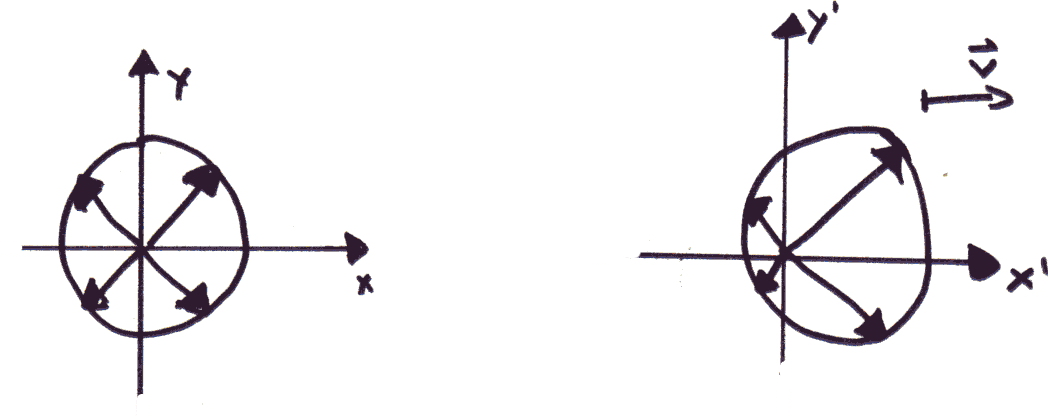
\includegraphics[scale=0.10]{Figs/Pim00013.png}
\end{center}
\end{wrapfigure}

$\longrightarrow$ Die Ausbreitungsgeschwindigkeit hängt von der Richtung ab! Dies steht im Widerspruch zu der aus den Maxwellgleichungen gefolgerten Wellengleichung. Eine der beiden Theorien muss also falsch sein. 

Dies ist im Widerspruch zum Experiment von Michelson und Morley (1887), welches zeigt, dass die Lichtgeschwindigkeit in \underline{allen} Inertialsystemen gleich ist.\\ \\
\underline{Lösung:} Einstein (1905) postuliert, dass die Lichtgeschwindigkeit in allen Inertialsystemen gleich ist.\\ \\
Konsequenzen:
\begin{itemize}
\item Die Galilei-Transformationen sind nicht mehr die korrekte Koordinatentransformation.
\item Die Newtonsche Mechanik ist nicht mehr gültig.
\item Die Zeitmessung hängt vom Inertialsystem ab. Die Zeit ist nicht mehr absolut.
\end{itemize}\vspace{1.5cm}
Beispielsweise sind die Maxwell-Gleichungen nicht invariant unter der Galilei-Transformationen.\\
\\
$\longrightarrow$ Einstein ersetzt die Galilei-Transformation durch die Lorentztransformation.\\

\subsubsection{Lorentztransformationen}
Gesucht ist die Transformation, die einen Lichtkegel invariant lässt:
\begin{eqnarray*}
\vec {r'}^2 - c^2 {t'}^2 = \vec r ^ 2 - c^2t^2
\end{eqnarray*}
Wir wählen den Ansatz einer linearen Transformation ($\vec r, t \rightarrow \vec r ',t'$) zwischen Inertialsystemem, die sich in x-Richtung mit einer Geschwindigkeit $\vec v$ gegeneinander bewegen.
\begin{alignat*}{5}
\text{Annahme:}\qquad \qquad &y' = y \qquad  \qquad \qquad \qquad \qquad  &z' \g z&\\
&t' = \gamma t- \gamma\beta \frac x c\qquad  &x' \g \gamma &x - \gamma\beta t \cdot c
\end{alignat*}
Der Ursprung sei bei $x' = 0$
\begin{eqnarray*}
\longrightarrow x = \beta c t  = v t \Rightarrow \boxed{\beta = \frac v c}\\
{\vec r}^{'2} -c^2{t}^{'2} = \vec r^2- c^2t^2 \Rightarrow \dots \Rightarrow\\
\boxed{\gamma = \frac1 {\sqrt{1 - \frac{v^2}{c^2}}} = \frac 1 {\sqrt{1- \beta^2}}}
\end{eqnarray*}
Dies sind die Lorentztransformationen (,,Boosts''):
\begin{eqnarray*}\boxed{
x' = \frac x  {\sqrt{1 - \frac{v^2}{c^2}}} - \frac{v t}{\sqrt{1 - \frac {v^2}{c^2}}}}\\\boxed{
t' = \frac t {\sqrt{1 - \frac{v^2}{c^2}}} - \frac{v \frac x{c^2}}{\sqrt{1 - \frac{v^2}{c^2}}}}
\end{eqnarray*}
Im Grenzfall $v\ll c$ wird aus den Lorentztransformationen die Galileitransformation und aus $t'$ wird $t$.

\vspace{1.5cm}
\underline{Transformationen im Minkowskidiagramm}\\
Die  Rücktransformation ist gegeben durch:
\begin{eqnarray*}
x = \gamma x' + \gamma \beta c t'\\
t = \gamma t' + \gamma \frac{\beta}  c x'
\end{eqnarray*}
Dies hat folgende physikalische Folgen:\\
\begin{wrapfigure}{l}{5.5cm}
\begin{center}
	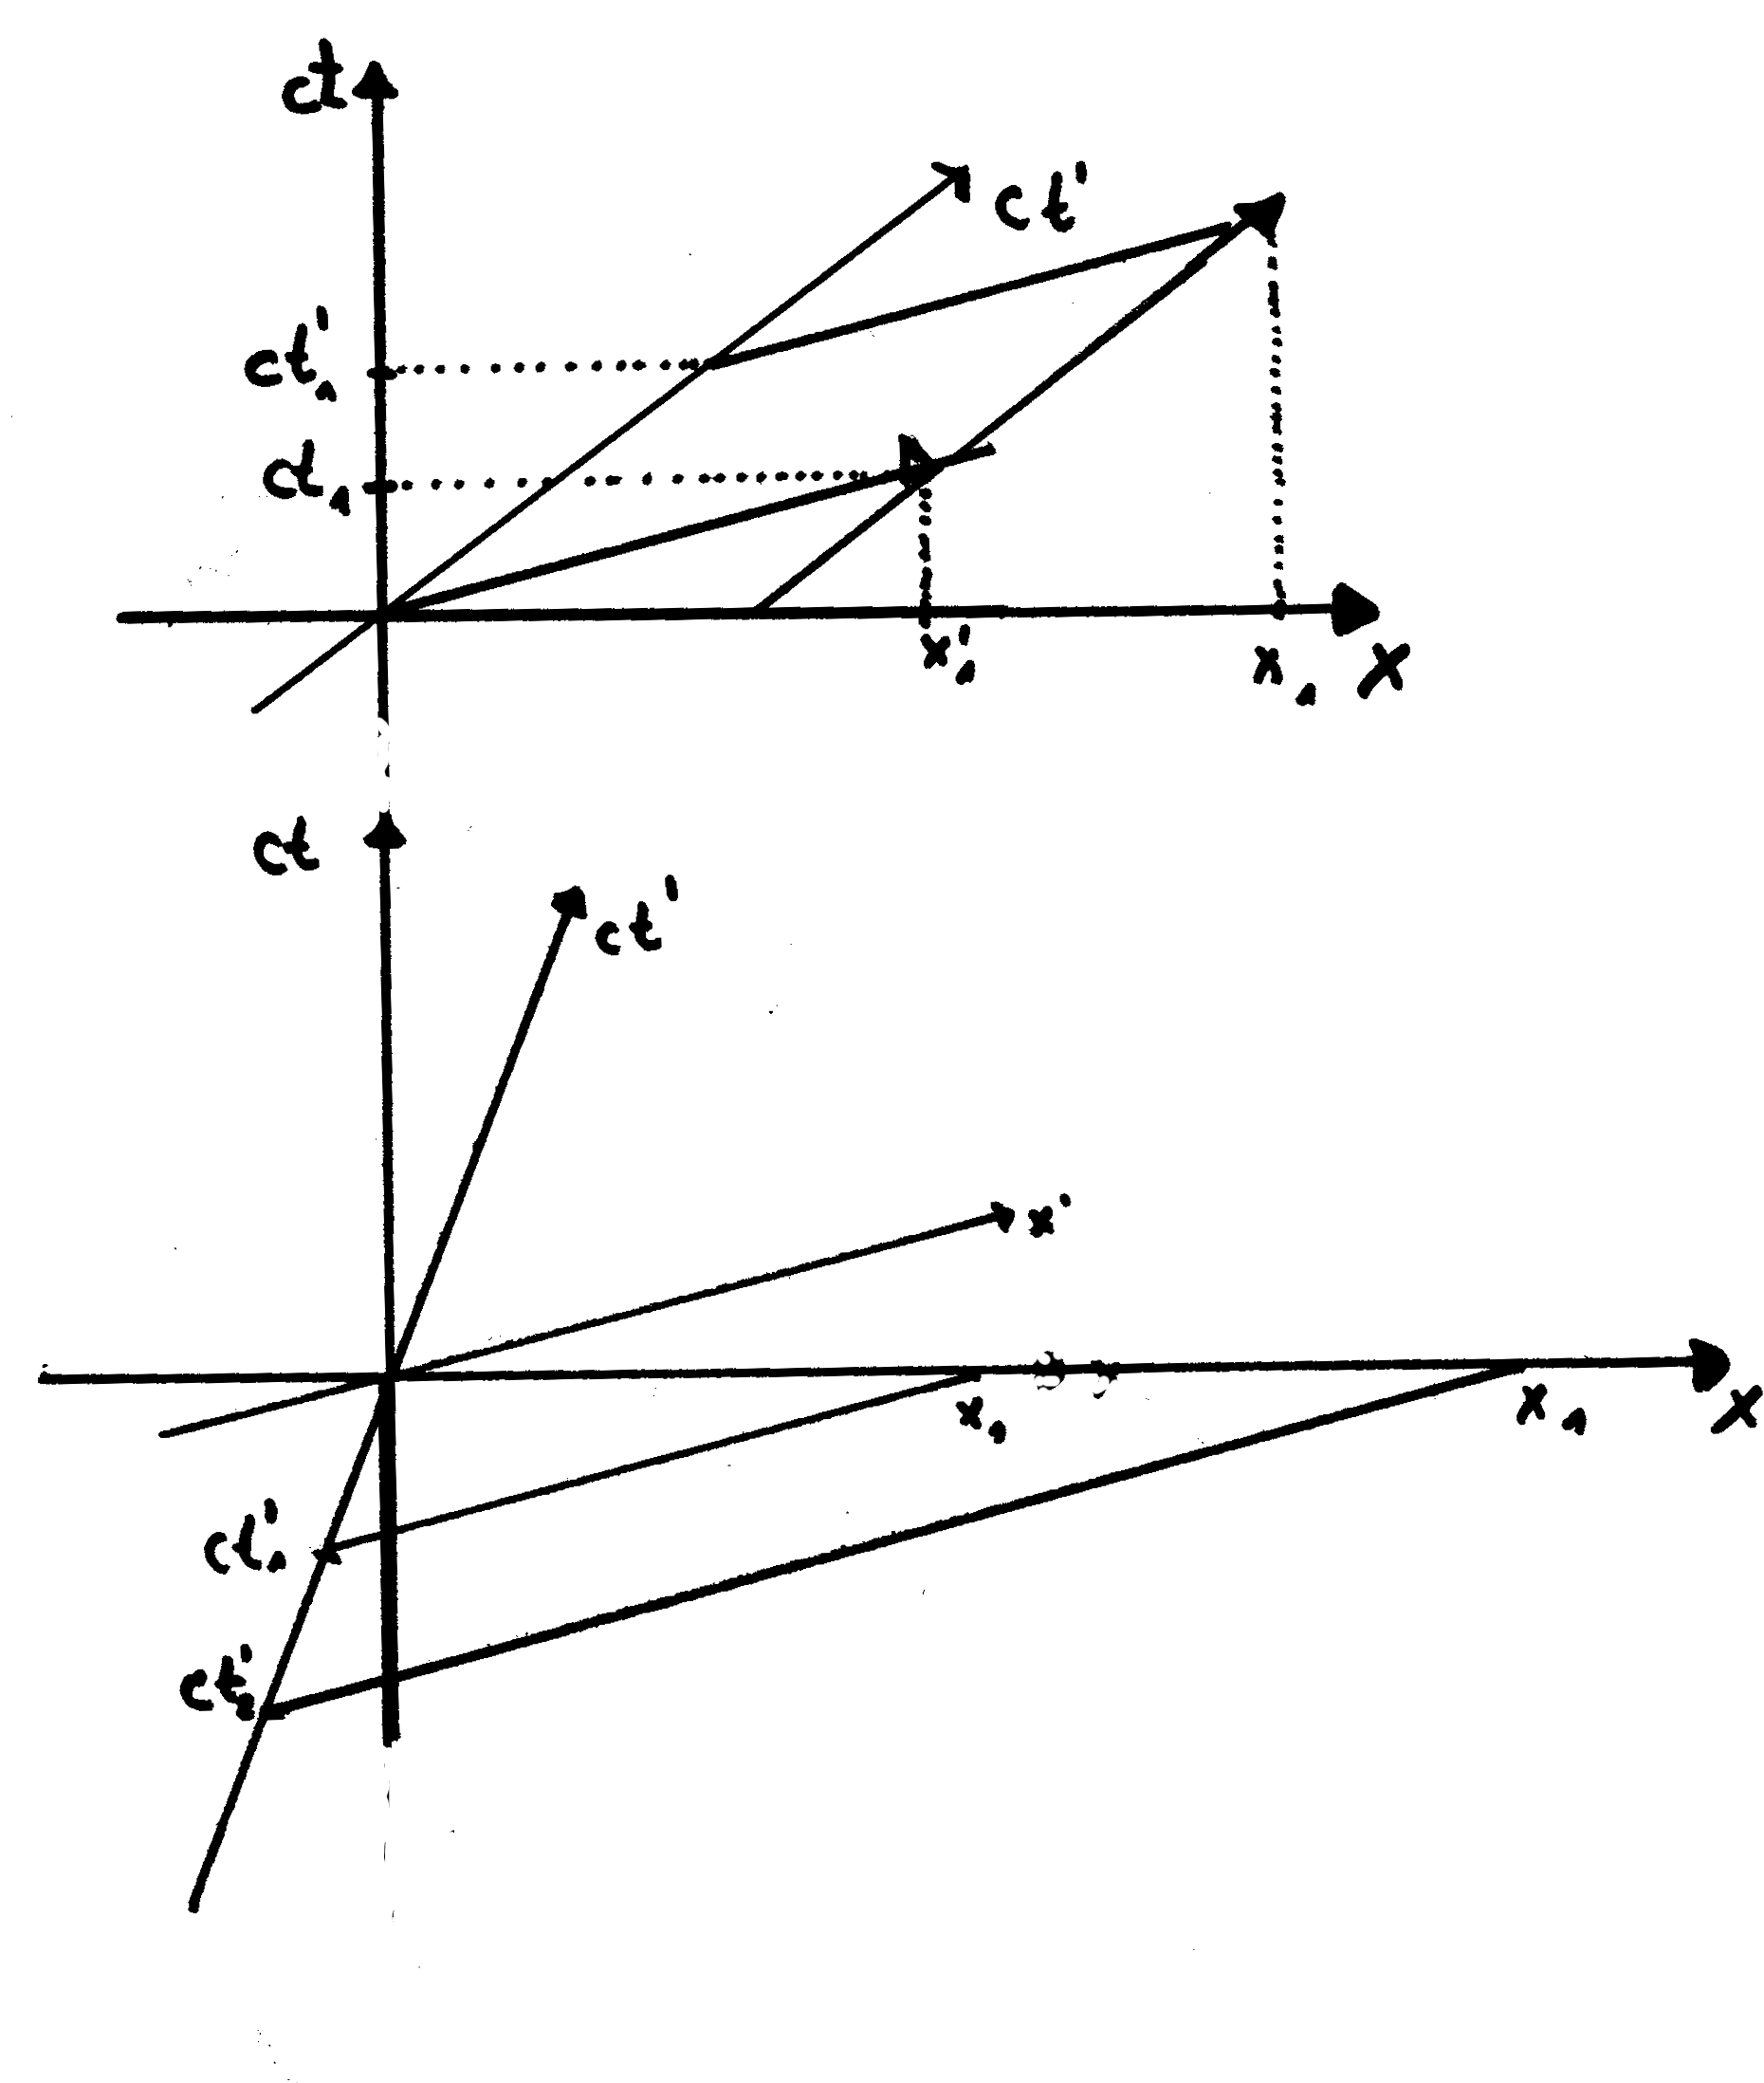
\includegraphics[scale=0.10]{Figs/Pim00012.png}
\caption{Minkowskidiagramm, unten: Relativität der Gleichzeitigkeit}
\end{center}
\end{wrapfigure}

\begin{itemize}


\item {Relativität der Gleichzeitigkeit:}\\
Zwei Ereignisse an verschiedenen Orten $x_1$ und $x_2$ zur Zeit $t=0$ im IS  sind nicht gleichzeitig im IS '.
\begin{eqnarray*}
t'_2-t'_1 \g -\beta \gamma \cdot \frac{(x_2-x_1)} c \neq 0\\
x'_2-x'_1 \g \gamma(x_2-x_1)\\
\Rightarrow (t'_2-t'_1) \g \frac {-\beta}c (x'_2-x'_1)
\end{eqnarray*}

\item {Zeitdilatation:}\\
Bei $x=0$ ist im IS' die Zeitdifferenz größer als im IS.
\begin{eqnarray*}
t'_2-t'_1 = \gamma(t_2-t_1) \ge t_2-t_1
\end{eqnarray*}

\item{Längenkontraktion:}\\
Der Wegunterschied $x_2-x_1$ ist zur Zeit $t'_2 = t'_1$  im IS'  geringer als im IS, d.h.\\ $x'_2-x'_1< x_2-x_1$.\\
\\




\begin{eqnarray*}
x'_2-x'_1 \g \gamma (x_2-x_1) - \beta\gamma(t_2-t_1) c\\
t'_2 - t'_1 = 0 \g \gamma (t_2-t_1) - \beta \gamma (x_2-x_1)\frac 1 c\\
\longrightarrow t_2-t_1 \g \beta \frac{(x_2-x_1) } c\\
\Longrightarrow x'_2 -x'_1 \g \gamma(1-\beta^ 2)(x_2-x_1) = \frac{(x_2-x_1)} {\gamma}
\end{eqnarray*}


\end{itemize}
\begin{center}
	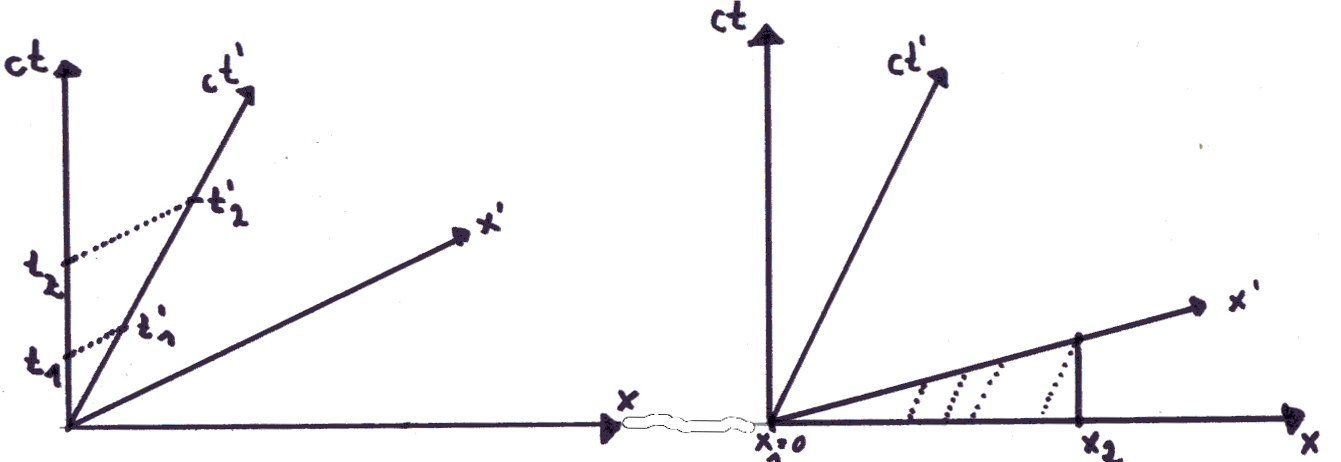
\includegraphics[scale=0.20]{Figs/Pim000111.png}
	\captionof{figure}{links: Zeitdilatation; rechts : Längenkontraktion}
\end{center}

\begin{itemize}
\item{ Kausalität bezüglich einem dem Ereignis im Ursprung}\\
Maximale Verschiebung liegt bei $ct = |\vec r| \ \ \ \rightarrow$ 45 \grat Verschiebung\\
$\Longrightarrow$ Lichtkegeloberfläche ist bei $|\vec r| = ct$\\
Ereignisse mit $|\vec r|^ 2<c^2 t^ 2$ befinden sich im Lichtkegel.\\
\begin{itemize}
\item Ereignisse mit $|\vec r|^ 2<c^2 t^ 2$ heißen {\bf zeitartig} und können mit $v<c$ erreicht werden.
\item Ereignisse mit $|\vec r|^ 2 > c^ 2t^ 2$ heißen {\bf raumartig} und können nicht erreicht werden.
\item Ereignisse mit $|\vec r| ^ 2 = c^2t^ 2$ heißen {\bf lichtartig} und können mit $v=c$ erreicht werden.

\begin{center}
	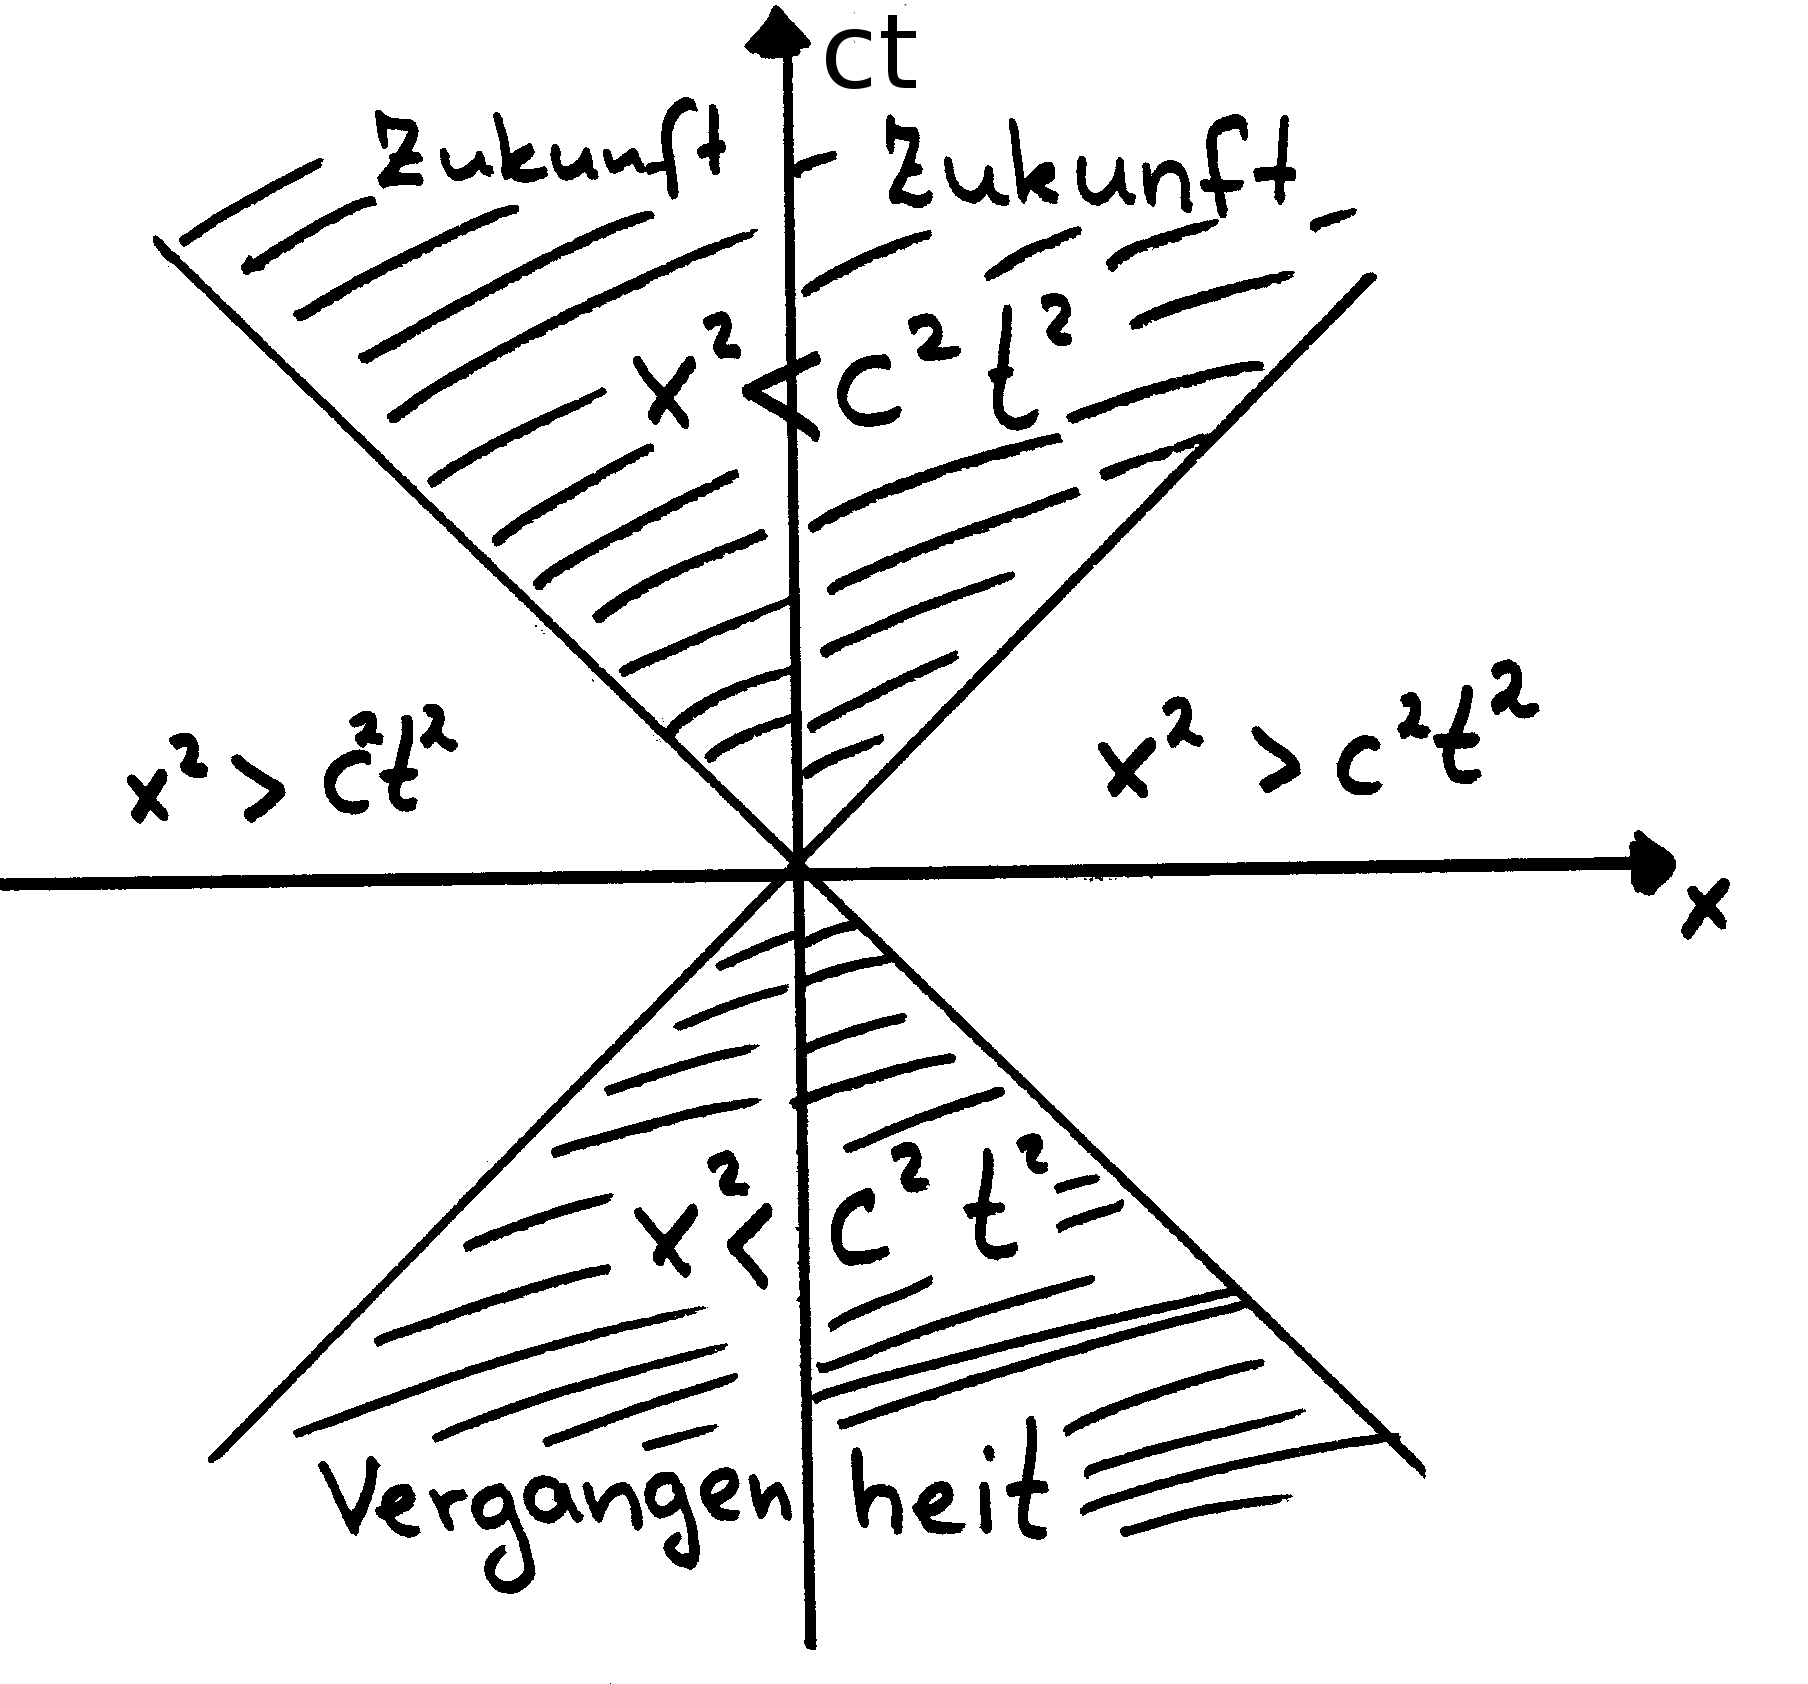
\includegraphics[scale=0.10]{Figs/Pim000112.png}
	\captionof{figure}{links: Zeitdilatation; rechts : Längenkontraktion}
\end{center}

\end{itemize}
Für Lorentztransformationen gilt: 
\begin{eqnarray*}
|\vec r|'^ 2-c^ 2t'^ 2 = |\vec r|^ 2- c^ 2t^ 2
\end{eqnarray*}
$\Longrightarrow$ Die Kausalität bleibt erhalten.
\end{itemize}

\subsubsection{Vierervektoren / Tensorrechnung}
Wir fassen Zeit und Raum zu einem sog. Vierervektor zusammen:
\begin{eqnarray*}
x \g (ct,x,y,z) = (x_0,x_1,x_2,x_3)\\
x^{\mu} \g \left ( \begin{array}{c} ct\\ x\\y\\z\end{array} \ri) = \left ( \begin{array}{c} ct\\ \vec r \end{array}\ri )
\end{eqnarray*}
Mit den Konventionen:
\begin{eqnarray*}
x^ 0 = c\cdot t \qquad x^ 1 = x \qquad x^ 2 = y \qquad x^ 2 = z
\end{eqnarray*}
\begin{center}
\begin{tabular}{cccccc}
\end{tabular}\end{center}
Lorentztransformationen lassen die Größe $c^ 2t^ 2 - \vec r^ 2$ invariant.\\
Definiere entsprechendes Skalarprodukt:
\begin{eqnarray*}
x^ 2_{\nu} = \sum \limits_{\mu = 0}^ 3 x^ {\mu} g_{\mu \nu} x^ {\nu} = c^ 2t^ 2- \vec r^ 2
\end{eqnarray*}
mit dem metrischen Tensor (Metrik):
\begin{eqnarray*}
g_{\mu\nu} = \left ( \begin{array}{cccc} +1&0&0&0\\0&-1&0&0\\0&0&-1&0\\0&0&0&-1\end{array} \ri)\\
g_{00} = 1 \qquad g_{ii} = -1 \qquad g_{\mu\nu} = 0 \text{ für  } \mu \neq \nu
\end{eqnarray*}
Definiere den kovarianten Vektor:
\begin{equation*}
 x_{\nu}=\sum_{\mu}g_{\mu\nu}x^{\mu}=(ct,-x,-y,-z)\quad\Rightarrow\quad x^2=\sum_{\nu}x_{\nu}x^{\nu}
\end{equation*}

\underline{Einsteinsche Summenkonvention}
Über wiederholt auftretende Indizes wird summiert.\\
Meist ist ein Index oben und einer unten gesetzt.\\
Lorentztransformation:
\begin{eqnarray*}
x'{}^{\mu} \g \Lambda^{\mu}_{\ \ \nu} \ \ x^{\nu}\\
\text{mit z.B. } \Lambda_{\ \ \nu}^{\mu} \g \left ( \begin{array}{cccc} \gamma&-\beta\gamma&0&0\\ -\beta \gamma&\gamma&0&0\\ 0&0&1&0\\0&0&0&1 \end{array} \ri)=\frac{\partial x'^{\mu}}{\partial x^{\nu}}
\end{eqnarray*}
Das Skalarprodukt ist invariant unter einer Lorentztransformation.
\begin{eqnarray*}
{x'}^2 \g {x'} ^{\mu} g_{\mu\nu} {x'}^{\nu} = x^{\lambda}\ \Lambda _{\ \ \lambda}^{\mu}\  \ g_{\mu\nu} \  \Lambda_{\ \ \kappa}^{\nu}\ \ x^{\kappa} \\ \g x^{\lambda} g_{\lambda \kappa} x^{\kappa}
\end{eqnarray*}
$\Longrightarrow$ Die Metrik ist in beiden Inertialsystemen die gleiche. (Dies folgt aus der Form der Lorentztransformation.)
\begin{itemize}
\item Es gilt ebenfalls:
\begin{eqnarray*} x \cdot y \g x^{\mu} \ g_{\mu\nu} \ y^{\nu} \\ \g x_0y_0 - x_1y_1-x_2y_2-x_3y_3 \end{eqnarray*}
\item Abstandsquadrat  $ds^2$\\
\begin{eqnarray*} ds^2 = dx^{\mu} \ g_{\mu \nu} dx^{\nu} = c^2dt^2 - d\vec r^2\end{eqnarray*}
Hieraus folgt, dass das Abstandsquadrat größer null, gleich null und kleiner null sein kann.\\
$\longrightarrow$ ,,pseudoeuklidischer Raum''
\end{itemize}
\vspace{1.5cm}
\underline{Verallgemeinerung der Vektoren auf {\bf Tensoren}.}
\begin{itemize}
\item {\bf Skalare (Tensoren 0. Stufe) }\\  Skalare ändern sich nicht unter einer Lorentztransformation ($s'(x') = s(x)$).\\
(Zum Beispiel : Skalarprodukt, Lichtgeschwindigkeit $c$, Ruhemasse,...)
\item {\bf Vektoren (Tensoren 1. Stufe)} Vektoren werden mit der Lorentztransformation transformiert.\\
Unterscheide zwischen:
\begin{itemize}
\item {\bf Kontravariante Vektoren}\\
\begin{eqnarray*} {A'}^{\mu} = \Lambda_{\ \ \nu}^{\mu} \ \ A^{\nu} \qquad \qquad
\big ( {x'}^{\mu} = \underbrace{\frac{\partial {x'}^{\mu}}{\partial x^\nu}}_{\Lambda_{\ \ \nu}^{\mu}} x^{\nu} \big)
\end{eqnarray*}
\item{\bf Kovariante Vektoren}\\ \begin{eqnarray*} B'_{\mu} = \Lambda_{\ \ \mu}^{\nu}\ \ B_{\nu} \qquad \qquad \big ( x'_{\mu} = \underbrace{\frac{\partial x^{\nu}}{\partial {x'}^{\mu}}}_{\Lambda_{\ \ \mu}^{\nu}}x_{\nu} \big )\end{eqnarray*}
\end{itemize}
Diese Vektoren können mit dem metrischen Tensor ineinander umgerechnet werden:
\begin{eqnarray*} B^{\mu} = g^{\mu\nu} B_{\nu}\end{eqnarray*}
Für das Skalarprodukt ergibt sich:
\begin{eqnarray*} AB = A^{\mu}B_{\mu} = A^{\mu} g_{\mu\nu} B^{\nu} \end{eqnarray*}
Als Beispiel kann der Vierervektor $x$ betrachtet werden:
\begin{eqnarray*}
x^{\mu} \g \Big ( ct, x,y,z \Big)\\ x_{\mu} \g g_{\mu\nu} B^{\nu} = \Big ( ct, -x,-y,-z\Big)
\end{eqnarray*}
Jedoch gilt für die Ableitungen:
\begin{alignat*}{6} \frac{\partial}{\partial x^{\mu}} \g \Big(\frac{\partial}{\partial ct}\ ,\frac{\partial}{\partial x} \ ,\frac{\partial}{\partial y}\ ,\frac{\partial}{\partial z} \Big ) \g \partial_{\mu} \qquad&\rightarrow& \quad \text{Kovariant}\\
\frac{\partial}{\partial x_{\mu}} \g \Big ( \frac{\partial}{\partial ct}\ ,\frac{-\partial}{\partial x}\ , \frac{-\partial}{\partial y}\ ,\frac{-\partial}{\partial z}\Big ) \g \partial^{\mu} \quad &\rightarrow& \quad \text{Kontravariant}
\end{alignat*}
Die obigen Gleichungen folgen aus der Umformung
\begin{eqnarray*} \frac{\partial}{\partial{x'}^{\mu}} = \underbrace{\frac{\partial x^{\nu}}{\partial{x'}^{\mu}}}_{\Lambda_{\ \ \mu}^{\nu}} \frac{\partial}{\partial x^{\nu}} \end{eqnarray*}
Die Divergenz ist wiederum ein Skalar $\partial_{\mu} A^{\mu} = \frac{\partial A^0}{\partial ct} + \nabla \vec A$

\item{\bf Tensoren höherer Stufe}\\
Tensoren der Stufe $k$ sind über ihr Transformationsverhalten unter $k$ Lorentztransformationen definiert.
\begin{eqnarray*}
{T'}^{\mu_1 \mu_2 \dots \mu_k} = \Lambda_{\ \ \nu_1}^{\mu_1} \ \ \Lambda_{\ \ \nu_2}^{\mu_2} \cdots \Lambda_{\ \ \nu_k}^{\mu_k}\ \ T^{\nu_1\nu_2\dots \nu_k} \end{eqnarray*}
$\longrightarrow$ Kontravariante Tensoren der $k$-ten Stufe (kovariant analog).\\ 
Für gemischte Terme gilt:
\begin{eqnarray*}
{T'}_{\ \ \ \  \ \ \ \ \mu_1 \dots\mu_k}^{\lambda_1 \dots \lambda_p} = \Lambda_{\ \ \mu_1}^{\nu_1} \cdots \Lambda_{\ \ \mu_k}^{\nu_k}\ \  \Lambda_{\ \ \kappa_1}^{\lambda_1}\cdots \Lambda_{\ \ \kappa_p}^{\lambda_p} \ \ T_{\ \ \ \ \ \ \ \nu_1 \dots\nu_k}^{\kappa_1 \dots \kappa_p}
\end{eqnarray*}
\underline{Beispiele:} \begin{itemize}
\item \begin{eqnarray*} T_{\mu\nu} ^{\ \ \ \ \ \lambda\delta}= x_{\mu}A_{\nu}\ x^{\lambda} B^{\delta}\end{eqnarray*}
\item Verjüngung eines Tensors \begin{eqnarray*} T_{\ \ \ \ \ \ \ \ \ \ \ \ \mu_1 \dots \mu_k}^{\nu_1 \dots \nu_{p-1} \mu_k}\end{eqnarray*}
Dies ist ein Tensor (mit $k-1$ kontra- und $p-1$ kovariante).
\begin{eqnarray*} &\rightarrow& \qquad  \qquad T_{\mu}^{\mu} = g_{\mu\nu} T^{\mu\nu} \quad \text{skalar} \\
&\rightarrow& \qquad\qquad x_{\mu}y^{\mu} = g_{\mu\nu}x^{\mu}y^{\nu} \end{eqnarray*}
\end{itemize}
\item{\bf D'Alembertoperator}
\begin{eqnarray*} 
\Box = \partial_{\mu} \partial^{\mu} = \frac 1 {c^2} \frac {\partial^2}{\partial t} - \frac{\partial ^2}{\partial \vec r^2} \ \widehat = \text{ skalare Größe}
\end{eqnarray*}
\item{\bf Invarianz vom Skalarprodukt}
\begin{eqnarray*} A'_{\mu} {B'}^{\mu} = \underbrace{\frac {\partial x^{\nu}}{\partial{x'}^{\mu}}\frac{\partial {x'}^{\mu}}{\partial x^{\gamma}}}_{= \frac{\partial x^{\nu}}{\partial x^{\gamma}}} A_{\nu}B^{\gamma} = A_{\nu}B^{\nu} \quad \text{mit } \frac{\partial x^{\nu}}{\partial x^{\gamma}} = \delta_{\gamma}^{\nu} = \delta_{\nu,\gamma}
\end{eqnarray*}
\item \begin{eqnarray*} g_{\mu\nu}g^{\nu\kappa} = g_{\mu}^{\kappa} = \delta_{\mu}^{\kappa} = \underbrace{\delta{(\kappa \mu)}}_{\text{Kronecker-}\delta}\end{eqnarray*}
\end{itemize}
\subsubsection{Relativistische Mechanik}
Die Newtonsche Mechanik ist nicht Lorentzkovariant, da Ableitungen nach der Zeit in der Newtonschen Mechanik auftreten, welche nicht kovariant sind.
\begin{eqnarray*} \frac{dx^ {\mu}}{dt} = \big ( c, \dot{\vec r} \big)\end{eqnarray*}
Die Konstruktion einer relativistischen Mechanik wird mit Hilfe der sog. {\bf Eigenzeit $\tau$} entwickelt. Diese Eigenzeit ist gleich der Zeit, die in einem mitbewegten Koordinatensystem vergeht:
\begin{eqnarray*}
c^2d\tau^2 \g c^2{dt'}^2 -\underbrace{d\vec {r'}^2}_{= 0} = c^2{dt}^2 - d\vec r^2\\
\g c^2dt^2\Big ( 1- \frac{\vec v(t)^2}{c^2} \Big) \qquad \text{mit }\vec v = \frac{d\vec r}{dt}
\end{eqnarray*}
\begin{eqnarray*}
\rightarrow \boxed{d\tau = \frac 1 {\gamma(t)} dt} \end{eqnarray*}
Beachte: In obiger Gleichung ist $\gamma$ von der Geschwindigkeit des Teilchens abhängig!
\underline{Definitionen:} 
\begin{itemize} \item{\bf Vierergeschwindigkeit}\\
\begin{eqnarray*}
\frac{dx^{\mu}}{d\tau} \g u^{\mu} = \frac{d}{d\tau} \big( ct, \vec r\big ) = \gamma \frac d{dt} \big( ct, \vec r\big)\\ \g \gamma(c,\vec v) \end{eqnarray*}
Der Betrag dieser Vierergeschwindigkeit $u_{\mu}$ ist gegeben durch
\begin{eqnarray*} u_{\mu}u^{\mu} = \gamma^2c^2 - \gamma^2v^2 = c^2.\end{eqnarray*}
\item{\bf Viererimpuls}\begin{eqnarray*} p^{\mu} = m \ u^{\mu}\end{eqnarray*}
\end{itemize}
\underline{Modifiziertes Newtonsches Gesetz}
\begin{eqnarray*}
\frac d{d\tau} p^{\mu} = m \frac{du^{\mu}}{d\tau} =: K^{\mu}
\end{eqnarray*}
Bestimmung der sog. {\bf Minkowskikraft} $K^{\mu}$\\
Betrachte die drei Raumkomponenten:
\begin{eqnarray*} m \frac {du^i}{d\tau} = \frac{dp^i}{d\tau} = \gamma \frac{dp^i}{d t} = \gamma F^i = K^i \end{eqnarray*}
und die Zeitkomponente:
\begin{eqnarray*} 
\underbrace{  m  u_{\mu} \frac{d u_{\mu}}{d\tau}}_{ = \ u_{\mu} K^{\mu}\ = \ u_0K^0 - \gamma\vec v\vec K} \g \frac m 2 \frac{d}{d \tau} u_{\mu}u^{\mu} = \frac m 2 \frac{d}{d\tau} c^2 = 0\\
\Longrightarrow K^0 \g \underbrace{\frac 1 {\gamma c}}_{= \frac 1 {u_0}} \gamma \vec v\vec K = \gamma \frac{\vec v\vec F} c.
\end{eqnarray*}
Mit der Forderung der Invarianz der Lorentztransformation lässt sich die Minkowskikraft mit $K^0$ bestimmen.
\begin{eqnarray*} \Longrightarrow K^{\mu} = \gamma \Big( \frac{\vec v\vec F}c , \vec F\Big )\end{eqnarray*}
\underline{Betrag des Viererimpulses $ p_{\mu}p^{\mu} = m^2 c^2$}\\
\begin{eqnarray*} 
cp^0 \g m\gamma c^2 = \frac{mc^2}{\sqrt{1 - \frac {v^2}{c^2}}} \quad\text{Entwickle nach $v$ für }v\ll c\\
\g \underbrace{mc^2}_{E_{\text{ruhe}}} + \underbrace{\frac 1 2m v^2 }_{\text{nicht relat. }E_{\text{kin}} } + \frac 3 8 m \frac{v^4}{c^2} + \dots
\end{eqnarray*}
$\longrightarrow$ Identifiziere $cp^0$ mit der Energie $E$.\\
$\longrightarrow$ Relativistischer Energie-Impuls Zusammenhang:
\begin{eqnarray*} \boxed{ E = \sqrt{m^2c^4 + c^2\vec p^2}}\end{eqnarray*}
Für ein Teilchen in Ruhe reduziert sich die Gleichung auf
\begin{eqnarray*} \boxed{E = mc^2}\end{eqnarray*}
und zeigt die Äquivalenz von Masse und Energie.


%%% Local Variables: 
%%% mode: latex
%%% TeX-master: "main"
%%% End: 
 \newpage
\thispagestyle{plain} \subsection{Kovariante Formulierung der Elektrodynamik}
Bisher wurde die Invarianz des Lichtkegels zur Herleitung der relativistischen Mechanik benutzt.\\
$\longrightarrow$ Lorentztransformation, Minkowskikraft.\\
$\longrightarrow$ Lichtwellenausbreitung bleibt invariant.\\ \\
\underline{Frage:} Wie sind die Transformationseigenschaften der Maxwellgleichungen ?\\
\subsubsection{Viererstrom}
\begin{itemize}
\item Wir gehen davon aus, dass die Ladung eines Punktteilchens ein Lorentzskalar ist.
\item Dies gilt jedoch nicht für die Ladungsdichte $\rho$, da das 3-dimensionale Volumen nicht Lorentzinvariant ist (Längenkontraktion).
\end{itemize}
Die Ladungsdichte und die Stromdichte hängen über die {\bf Kontinuitätsgleichung} zusammen.
\begin{eqnarray*} \frac{\partial}{\partial t} \rho + \nabla \vec j = 0 \end{eqnarray*}
\underline{Definition:} {\bf Viererstrom} $j^{\mu} = \big ( c\rho, \vec j\big)$\\
Daraus folgt \begin{eqnarray*} \partial_{\mu}j^{\mu}  = 0 .\end{eqnarray*}
Die  Kontinuitätsgleichung ist Lorentzinvariant. Anschaulich lässt es sich so betrachten, dass die ruhende Ladung im Inertialsystem IS der Stromdichte im Inertialsystem IS' entspricht.

\subsubsection{Viererpotential}
\begin{eqnarray*} A^{\mu}  \g \Big ( \frac{\phi}c,\vec A \Big )\\
\phi \g \text{skalares Potential}\\
\vec A \g \text{Vektorpotential}\\
\end{eqnarray*}
Das Viererpotential kann aus den Maxwellgleichungen hergeleitet werden.\\
\begin{equation}\label{eq4}
\vec E = - \grad (\phi) - \dot{\vec A} \qquad \qquad \vec B = \rot( \vec A)
\end{equation}
Schreibe die inhomogenen Maxwell-Gleichungen mit den Potentialen (\ref{eq4}) anstelle der $\vec E $- und $\vec B$-Felder.
\begin{eqnarray*}
\divergenz \vec E \g -\Delta \phi - \divergenz\dot{\vec A} = \frac{\rho}{\varepsilon_0}\\
\rot \vec B - \frac 1 {c^2} \dot{\vec E} \g \grad \ \divergenz \vec A - \Delta \vec A + \frac 1 {c^2} \grad \dot \phi + \frac 1 {c^2} \ddot{\vec A } = \mu_0 \vec j
\end{eqnarray*}
Zur Vereinfachung wird die folgende Eichtransformation durchgeführt.
\begin{eqnarray*} \text{wähle }\frac 1 {c^2 } \dot \phi + \divergenz \vec A \g 0 \text{  (Lorentzbedingung)}\\
\Rightarrow -\Delta \phi + \frac 1 {c^2} \ddot \phi \g \frac{\rho}{\varepsilon_0} = \mu_0 c^2 \rho\\
\Rightarrow -\Delta \vec A + \frac 1 {c^2} \ddot{\vec A} \g \mu_0 \vec j
\end{eqnarray*}
Die obigen Gleichungen haben die Form von Wellengleichungen, daher benutzen wir den \\ d'Alembertoperator $\square$, um diese auszudrücken. 
\begin{eqnarray*}
\Box  = \frac 1 {c^2} \partial_t^2 - \Delta \quad \quad \text{ist Lorentzskalar}\\
\Longrightarrow \text{  Viererpotential:}\qquad A^{\mu} = \Big ( \frac{\phi}c , \vec A \Big )
\end{eqnarray*}
Die inhomogenen Maxwellgleichungen sind  explizit kovariant:
\begin{eqnarray*}
\Box A^{\mu} \g \mu_0 j^{\mu}\\
\partial_{\mu} A^{\mu} \g 0 \qquad \widehat = \text{  Lorenzbedingung}
\end{eqnarray*}


\subsubsection{Feldstärketensor}
\begin{alignat*}{7}
&\vec B &=& \nabla \times \vec A \qquad \qquad \qquad &\vec E  \ \ &=& -\nabla \phi - \dot{\vec A}\\
&B_x &=& \partial_yA_z-\partial_zA_y \qquad\qquad\qquad &E_x &=& -\partial_x\phi - \partial_tA_x\\
&{}&=& -\partial^2A^3+ \partial^3A^2\qquad\qquad\qquad &{} &=& \ \partial^1A^0c - \partial^0A^1c
\end{alignat*}
Die rechten Seite hat die Form eines zweistufigen Tensors:\begin{eqnarray*}\boxed{F^{\mu\nu} = \partial^{\mu}A^{\nu}-\partial^{\nu}A^{\mu}} \quad \widehat = \ \ \text{\bf Feldstärketensor}\end{eqnarray*}
Ein antisymmetrischer Tensor 2. Stufe besitzt 6 freie Komponenten:
\begin{eqnarray*}
F^{\mu\nu} = \left ( \begin{array}{cccc} 0	& \frac{-E_x}c	&\frac{-E_y}c	&\frac{-E_z}c\\
				\frac{E_x}c	& 0		&-B_z		&B_y\\
				\frac{E_y}c	& B_z		& 0 		& -B_x\\
				\frac{E_z}c	&-B_y		&B_x		&0 \end{array}\ri)
\end{eqnarray*}\\
Der kovariante Feldstärketensor ergibt sich zu:
\begin{eqnarray*}
F_{\mu\nu} = g_{\mu\lambda}g_{\nu\kappa}F^{\lambda \kappa} =
 \left ( \begin{array}{cccc}            0       & \frac{E_x}c	&\frac{E_y}c	&\frac{E_z}c\\
				\frac{-E_x}c	& 0		&-B_z		&B_y\\
				\frac{-E_y}c	& B_z		& 0 		& -B_x\\
				\frac{-E_z}c	&-B_y		&B_x		&0 \end{array}\ri)
\end{eqnarray*}
Die Vorzeichen ergeben sich durch die Regeln
\begin{center}
	\begin{tabular}{cccccc}
		$\lambda \kappa$ &sind beide raumartig& $\rightarrow$ & $(-1) \cdot (-1)$ & $\rightarrow$& +1 \\
		$\lambda \kappa$ &sind beide zeitartig & $\rightarrow$& $(+1) \cdot (+1)$ & $\rightarrow$& +1 \\
		 $\lambda \kappa$ &eines ist zeit-, das andre raumartig & $\rightarrow$ & $(-1) \cdot (+1)$& $\rightarrow$ & -1 \\
	\end{tabular}
\end{center}

\underline{Definitionen}
\begin{itemize}
\item{\bf Total asymmetrischer Tensor 4. Stufe}
\begin{eqnarray*}
\varepsilon^{\alpha \beta\gamma\delta} = \left \{ \begin{array}{cc} +1 & \text{für }\alpha = 0, \beta = 1, \gamma= 2, \delta = 3\\&\text{und gerade Permutationen}\\ -1 &\text{für ungerade Permutationen}\\ 0 &\text{sonst} \end{array} \ri.
\end{eqnarray*}
\item{\bf Dualer Feldstärketensor}
\begin{eqnarray*} \boxed{ \tilde{F}^{\alpha\beta} = \frac 1 2 \varepsilon^{\alpha\beta\gamma\delta} F_{\gamma\delta}}
\end{eqnarray*}
Explizit ist der duale Feldstärketensor:
\begin{eqnarray*} \tilde F^{\alpha\beta} = \left ( \begin{array}{cccc}
 0	&	-B_x	&	-B_y	&	 -B_z\\
B_x	&	0	&	\frac{E_z}c	&-\frac{E_y}c\\
B_y	&	-\frac{E_z}c	&	0	&\frac{E_x}c\\
B_z	&	\frac{E_y}c	&-\frac{E_x}c	&	0
\end{array}\ri )
\end{eqnarray*}
\end{itemize}
\underline{Maxwellgleichungen:}
\begin{itemize}
\item{Inhomogen}
\begin{eqnarray*}
\underbrace{\nabla \vec E}_{\partial_{\mu}F^{\mu 0}c} = \underbrace{\frac{\rho}{\varepsilon_0}}_{\mu_0j^0c}\qquad \qquad \underbrace{\nabla \times \vec B}_{\partial_iF^{i j}} - \underbrace{\frac 1 {c^2}\dot{\vec E}}_{-\partial_oF^{0 j}} = \underbrace{\mu_0 \vec j}_{\mu_0 j^j}
\end{eqnarray*}
\begin{eqnarray*}\Rightarrow\boxed{\partial_{\mu}F^{\mu\nu} = \mu_0j^{\nu}}\end{eqnarray*}

\item{homogen}
\begin{eqnarray*} \nabla \times \vec E + \dot{\vec B} = 0 \qquad\qquad \nabla \vec B = 0\end{eqnarray*}
Mit Hilfe des dualen Feldstärketensors lassen sich die homogenen Maxwellgleichungen in einer Gleichung zusammenfassen.
\begin{eqnarray*} \boxed{ \partial_{\mu}\tilde F^{\mu\nu} = 0}\end{eqnarray*}
Eine äquivalente Formulierung ist:
\begin{eqnarray*} \partial^{\lambda} F^{\mu\nu} + \partial^{\mu}F^{\nu\lambda} + \partial^{\nu}F^{\lambda\mu} = 0\end{eqnarray*}
$\Longrightarrow$ Explizite kovariante Form der Maxwellgleichungen.

\end{itemize}





\underline{Transformationsverhalten der Felder}\\
Feldstärketensor: ${F'}^{\mu\nu} = \Lambda_{\kappa}^{\mu}\Lambda_{\delta}^{\nu}F^{\kappa \delta}$\\
Für einen Boost in $x$-Richtung ergibt sich 
\begin{eqnarray*} \Lambda_{\nu}^{\mu} = \left ( \begin{array}{cccc}
\gamma		& -\beta \gamma		&0	&0\\
-\beta\gamma	&\gamma			&0	&0\\
0		&0			&1	&0\\
0		&0			&0	&1 \end{array}\ri)
\end{eqnarray*}
						
Es gilt:
\begin{eqnarray*}
E'_x \g E_x \qquad \qquad B'_x = B_x\\
E'_y \g \gamma E_y  - \beta\gamma B_z c\\
B'_y \g \gamma B_y  +\beta\gamma \frac{E_z}c\\
E'_z \g \gamma E_z  + \beta\gamma B_y c\\
B'_z \g \gamma B_z  - \beta\gamma \frac{E_y}c
\end{eqnarray*}
$\longrightarrow$ Felder in $x$-Richtung bleiben unverändert.\\
Felder senkrecht zur $x$-Richtung: $\vec E$- und $\vec B$-Feld Komponenten werden gemischt.\\ \\
\underline{Beispiel:} Statisches Feld $E_y$ (sonst in Komponenten $=0$)\\
\begin{eqnarray*}
\rightarrow E'_y = \gamma E_y\qquad\qquad B'_z = -\beta\gamma\frac{E_y}c = -\beta \frac{E'_y}c\\
\rightarrow \vec B\perp\vec E \text{  und  } \perp \vec v
\end{eqnarray*}
Das $\vec B$-, $\vec E$-Feld und der Geschwindigkeitsvektor $\vec v$ stehen allgemein immer senkrecht zueinander in der Elektrostatik.\\ Es gilt:
\begin{eqnarray*} \vec B' = \vec v \times \frac{\vec E'}{c^2} \end{eqnarray*}


\subsubsection{Geladenes Teilchen}
Lorentzkraft ist $\vec F = q\big(\vec E + \vec v\times \vec B \big)$.\\
Die Minkowskikraft ist gegeben durch:
\begin{eqnarray*}
K^{\mu} \g \gamma q \big ( \vec v \frac{\vec E}c, \vec E + \vec v \times \vec B \big)\\
\g q \big( \vec u \frac{\vec E}c , u_0 \frac{\vec E}c + \vec u \times \vec B\big)\\
&{}&\text{mit }u^{\mu} = \gamma(c,\vec v)
\end{eqnarray*}
\begin{eqnarray*}
\text{d.h.}\quad \frac{dp_0}{d\tau} \g \frac q c \vec u\cdot\vec E\qquad \text{Energieänderung}\\
\frac{d\vec p}{d\tau} \g q \Big ( u_0 \frac{\vec E} c + \vec u\times \vec B\Big )
\end{eqnarray*}
Die rechte Seite kann geschrieben werden als:
\begin{eqnarray*}\boxed{\frac{dp^{\mu}}{d\tau} = qF^{\mu\nu}u_{\nu}}\end{eqnarray*}
$\longrightarrow$ Das Gleichungssystem ist \underline{kovariant} geschlossen.
\begin{eqnarray*}
\partial_{\mu} F^{\mu\nu} \g \mu_0 j^\nu\\
\partial_{\mu}\tilde F^{\mu\nu} \g 0\\
m\frac{du^{\mu}}{d\tau} \g q F^{\mu\nu} u_{\nu}\\
&{}&\longrightarrow  u^{\mu} \text{   bestimmt   }j^{\mu}
\end{eqnarray*}

%%% Local Variables: 
%%% mode: latex
%%% TeX-master: "main"
%%% End: 
 \newpage
\thispagestyle{plain} \subsection{Lagrangeformalismus}
\subsubsection{Mechanik eines freien Teilchens}
Die Wirkung ist $S = \int \Lr(q,\dot q,t)dt$.\\
\underline{Problem:} $dt$ ist nicht kovariant.\\
\underline{Lösung:} Wir führen die Eigenzeit $d\tau = \frac{dt}{\gamma}$ ein.
\begin{eqnarray*} \longrightarrow S_{\text{frei}} =\int \gamma \Lr_{\text {frei}}d\tau \end{eqnarray*}
Damit das Prinzip der kleinsten Wirkung gilt, muss $S$ (und damit $\delta S = 0$) ein Skalar sein! Da ein freies Teilchen orts- und richtungsunabhängig ist, ist der einzige geschwindigkeitsabhängige Skalar der Geschwindigkeitsbetrag:
\begin{eqnarray*} \text{mit  } u_{\mu}u^{\mu} = c^2\\ \Longrightarrow S \g - \int mc^2d\tau \\
\text{bzw. } S \g \int - \underbrace{m c^2 \sqrt{1 - \frac{\vec v ^2}{c^2}}}_{\Lr_{\text{frei}}=\sqrt{u_{\mu}u^{\mu}}mc}dt\end{eqnarray*}
Beachte: $u_{\mu}u^{\mu}$ darf erst nach Variation verwendet werden, da $u^0(\tau)=\frac{\text{d}t}{\text{d}\tau}$ erst als unabh‰ngige Funktion ausgerechnet werden muss.
Dies ergibt:
\begin{eqnarray*}
\frac d{dt} \frac{\partial \Lr}{\partial v_i} = \frac d {dt} m \gamma \vec v = 0 \qquad \widehat = \text{ konst. Geschwindigkeit}\end{eqnarray*}
\subsubsection{Mechanik mit elektromagnetischem Feld}
\begin{eqnarray*} \Lr = \Lr_{\text{frei}} + \Lr_{\text{int}} \qquad \text{mit  }\gamma\Lr \wh = \text{  Skalar}\end{eqnarray*}
Forderungen an $\Lr_{\text{int}}$ (neben der Kovarianz)
\begin{itemize}
\item Linear in der Ladung $q$
\item Linear in dem Potential $A^{\mu}$
\item Translationsinvariant ( explizit unabhängig von $x^{\mu}$ )
\item Möglichst Funktionen 1. Ableitung
\end{itemize}
\begin{eqnarray*}\longrightarrow \Lr_{\text{int}} \g - q u_{\mu} \frac{A^{\mu}}{\gamma} \\
\g - q \phi + q \vec v\vec A\\
\end{eqnarray*}
\begin{eqnarray*}
\Longrightarrow \boxed{ \Lr = -mc^2 \sqrt{1 - \frac{\vec v^2}{c^2}} + q \vec v\vec A - q \phi}
\end{eqnarray*}
\underline{Kanonische Impulse:}
\begin{eqnarray*}
\vec p_{\text{kan}} = \frac{\partial \Lr}{\partial \vec v} = m\gamma\vec v + q \vec A\\
\Longrightarrow \vec v = c ^2\frac{\vec p - q \vec A}{\sqrt{m^2c^4 + c^2(\vec p - q\vec A)^2}}
\end{eqnarray*}
\underline{Hamiltonfunktion:}
\begin{eqnarray*}
\ham = \sqrt{m^2c^4 + c^2(\vec p-q\vec A)^2} + e\phi \end{eqnarray*}
\underline{Bemerkung:} \babsatz Der Hamiltonformalismus kann nicht mehr mit der Energie identifiziert werden, da die Hamiltonfunktion nun ein Lorentzskalar ist und die Energie die Zeit-Komponente eines Vierervektors sein sollte.\eabsatz \vspace{0.5cm}

\underline{Kovariante Form der Lagrangefunktion}\\
Mit Hilfe der Vierer-Geschwindigkeit 
\begin{eqnarray*}
\sqrt{1 - \frac{\vec v^ 2}{c^ 2}} = \frac 1 { \gamma} \frac{u_{\mu} u^ {\mu}}{c^2}
\end{eqnarray*}
und der Eigenzeit $d\tau = \gamma dt$ lässt sich die Wirkung umschreiben:
\begin{eqnarray*}
S_{\text {frei}} = -mc \int \sqrt{u_{\mu}u^ {\mu }} d\tau\\
\text{mit Zwangsbedingung}\qquad u_{\mu}u^ {\mu} = c^ 2\\
\Longrightarrow \quad S_{\text{frei}} = \text{ const.}
\end{eqnarray*}
Ausweg: \babsatz  Wir führen ein Bahnparameter ($s$) ein, der \underline{nach} der Variation nach $ds = cd\tau$ mit der Eigenzeit identifiziert wird.\\
(D.h. $ \frac{dx^ {\mu}}{ds}\frac {dx_{\mu} }{ds} \neq 1$.)\eabsatz
\begin{eqnarray*}
\Longrightarrow S_{\text{frei}} = -mc \int \sqrt{g_{\mu\nu}\frac{dx^ {\mu}}{ds} \frac{dx^{\nu} }{ds} }ds\\
\text{Für die Ww. Mit dem e.m-Feld gilt:}\\
S_{\text{int}} = - q \int \frac{dx^ {\mu}}{ds} A_{\mu}(x) ds
\end{eqnarray*}
die Variation von $S_{\text{frei}} + S_{\text{int}}$ mit $ds = cd\tau$ und $u_{\mu}u^ {\mu} = c^ 2$ ergibt:
\begin{eqnarray*}
\Longrightarrow&{}& m \frac{d^ 2x^ {\mu}}{d\tau^ 2} + q
\underbrace{\frac{dA^ {\mu}}{d\tau}}_{=
  \frac{dx_{\nu}}{d\tau}\partial^ {\nu}A^ {\mu}} - q\frac{dx_{\nu}}{d\tau} \partial^ {\mu} A^ {\nu} = 0\\ 
\text{mit }&{}& \quad \big ( \partial^  {\nu}A^ {\mu} - \partial^ {\mu}A^ {\nu}\big ) = F^ {\nu\mu}\\
\g m \frac{d^ 2x^ {\mu}}{d\tau^ 2} + q \frac{dx_{\nu}}{d \tau} F^ {\nu\mu} = 0
\end{eqnarray*}
\subsubsection{Felder}
Behandlung von Feldern im Lagrangeformalismus: Fasse die Felder $\phi_k(x)$ als ,,k-te Koordinate eines Freiheitsgrades bei $x^\mu$ auf. Hierbei ist $x$ der Viererortsvektor.\\
In 4-Dimensionen ergibt dies:



\begin{center}
\begin{tabular}{ccc|c}
 & &Hier&Klassisch\\
Kontinuierlicher Index/Indizes&$\longrightarrow$&$x^ {\mu}$&$t$\\
Auslenkung&$\longrightarrow$&$\phi_k(x)$&$x(t)$\\
Geschwindigkeit&$\longrightarrow$&$\partial^ {\mu}\phi_k(x)$&$\partial_t x(t)$
\end{tabular}
\end{center}

Die Wirkung ist
\begin{eqnarray*}
S = \int d^ 4x \Lr\big(\phi_k,\partial ^ {\mu}\phi_k\big)
\end{eqnarray*}
Die Euler-Lagrangegleichung ergibt sich zu:
\begin{eqnarray*}
\partial^ {\mu} \frac{\partial \Lr}{\partial ( \partial^ {\mu}\phi_k)} - \frac{\partial \Lr}{\partial \phi_k} = 0
\end{eqnarray*}
\begin{itemize}
\item $k$ partielle Differentialgleichungen für $\phi_k(x)$.
\item $\Lr \wh =$Lagrangedichte.
\item $dx^ 4$ ist ein Lorentzskalar $\longrightarrow$ $\Lr$ muss ebenfalls ein Lorentzskalar sein.
\end{itemize}
Anwendung auf die Elektrodynamik:
\begin{itemize}
\item Freie Felder (Felder ohne Quellen) betrachten vier Potentiale ($A^ {\mu}$)\\
$\longrightarrow \ \Lr$ hängt nur von den Ableitungen ab.
\item Die Kopplung an der Materie ist linear in $A^ {\mu}$.
\end{itemize}
Ansatz:
\begin{eqnarray*} \boxed{ \Lr = \frac {-1}{4\mu_0} F_{\mu\nu}F^ {\mu\nu} - j_{\mu} A^ {\mu}}\end{eqnarray*}
Es gilt die Euler-Lagrangegleichung:
\begin{eqnarray*} \frac{\partial \Lr}{\partial A^ {\mu}}\g - j_{\mu}\\
\rightarrow -4\mu_0 \frac{\partial \Lr}{\partial\big ( \partial^ {\nu}A^{\mu}\big)} \g \frac{\partial}{\partial \big(\partial^ {\nu}A^{ \mu}\big)} g_{\alpha\beta}g_{\gamma\delta}F^ {\alpha\gamma}F^{\beta\delta}\\
\g g_{\alpha\beta}g_{\gamma\delta}\frac{\partial}{\partial\big(\partial^{\nu}A^{\mu}\big)} \Bigg[\Big( \underbrace{\partial^{\alpha}A^{\gamma}-\partial^{\gamma}A^{\alpha}}_{=F^{\alpha\gamma}}\Big)\Big(\underbrace{\partial^ {\beta}A^ {\delta}-\partial^ { \delta}A^ {\beta}}_{=F^{\beta\delta}}\Big)\Bigg]\\
\text{mit } \frac{\partial \big (\partial^ {\alpha}A^ {\gamma}\big )}{\partial\big(\partial^ {\nu}A^ {\mu}\big )} = \delta_{\nu}^ {\alpha}\delta_{\mu}^ {\gamma}\\
\g g_{\alpha\beta}g_{\gamma\delta} \Bigg[\Big(\delta_{\nu}^ {\alpha}\delta_{\mu}^ {\gamma}-\delta_{\nu}^ {\gamma}\delta_{\mu}^ {\alpha}\Big) F^ {\beta\delta} + \Big(\delta_{\nu}^ {\delta}\delta_{\mu}^ {\delta} - \delta_{\nu}^ {\delta}\delta_{\mu}^ {\beta}\Big )F^ {\alpha\gamma} \Bigg]\\
\g F_{\nu\mu}-F_{\mu\nu}+F_{\nu\mu}-F_{\mu\nu} = 4 F_{\nu\mu}\\
\Longrightarrow &{}& \boxed{\partial^ {\mu}F_{\mu\nu} = \mu_0 j_{\nu}}
\end{eqnarray*}
Die obige Gleichung ist die inhomogene Maxwellgleichung.\\
Die homogenen Maxwellgleichungen sind durch den Ansatz $F^ {\mu\nu} = \partial^ {\mu}A^ {\nu}-\partial^ {\nu}A^ {\mu}$ automatisch erfüllt.\\
Es gilt ebenfalls:
\begin{eqnarray*}
\underbrace{\partial^{\nu}\partial^{\mu}F_{\mu\nu}}_{\partial^ {\nu}\partial^ {\mu}=\partial^ {\mu}\partial^ {\nu} \text{ aber }F^ {\mu\nu}= -F^ {\nu\mu}} = -\mu_0\partial^ {\nu}j_{\nu}
\end{eqnarray*}
$\Longrightarrow \partial^ {\nu} j_{\nu} = 0$ Die Kontinuitätsgleichung ist erfüllt.\\


\subsubsection{Felder und Teilchen}
Für ein Teilchen $i$ mit \{$x_{(i)}^{\mu}(\tau)$\} und Felder $F^ {\mu\nu}(x^ {\mu})$ gibt es eine Lagrangefunktion mit dem Wechselwirkungsterm
\begin{eqnarray*} \int ds \ q \frac{dx^ {\mu}} {d s}\ A_{\mu}\left(x(s)\ri) \leftrightarrow \int d^4x \ j_{\mu}(x)A^ {\mu}(x).\end{eqnarray*}
Die Stromdichte für ein Teilchen ist
\begin{eqnarray*} j^ {\mu}(x) = \sum_i\int ds \ q_i \frac{dx^ {\mu}}{d s}\delta^ {(4)}(x-x_i(s)). \end{eqnarray*}
Einsetzen ergibt den obigen Wechselwirkungsterm, wobei $s$ mit $\tau$ identifiziert werden kann.
Ebenso ist die Lagrangefunktion für ein freies Teilchen
\begin{eqnarray*}
\Lr_{\text{frei}}\left( \frac{dx}{ds}\ri) = \int d^ 4x' \Lr \left( \frac{dx'}{ds}\ri )\delta^ {(4)}(x'-x(s)).\end{eqnarray*}
Die gesamte relativistische Mechanik und Elektrodynamik ist bestimmt durch:
\begin{eqnarray*}
S \g \int d^4x \ \Lr \left ( \Big\{x_i, \partial^{\mu}x_i\Big \} ,A^{\mu}(x),\partial^{\mu} A^{\nu}(x) \ri )\\
\Lr \g \sum \limits_i - m_ic \int d\tau \delta^{(4)}(x-x_i(\tau))\sqrt{u_{i}^{\mu}u_{i\;\mu}}\\ &{}& - \sum\limits_i q_i \int d\tau \frac{dx_{i}^{\mu}(\tau)}{d\tau} \delta^{(4)}\big(x-x_{i}(\tau)\big)A_{\mu}(x) \\&{}& -\frac 1 {4 \mu_0}F_{\mu\nu}F^{\mu\nu}
\end{eqnarray*}
\begin{itemize}
\item Variation von $S$ nach $x_i(s_i)$ und $A_{\mu}(x)$ ergibt die Bewegungsgleichung der Teilchen und die Maxwellgleichungen.
\item Die Beschreibung der effektiven Wechselwirkung zwischen den Teilchen wird nicht einfach sein, da die Potentiale von dem Ort der Teilchen zu retardierten Zeiten abhängen. $\longrightarrow$ nicht instantane Wechselwirkung.
\item In niedrigster relativistischer Ordnung $\longrightarrow$ Darwin Terme (siehe Übung).
\end{itemize}
\subsubsection{Energie-Impuls- oder Spannungstensor}
Für eine allgemeine Feldtheorie gilt:
\begin{eqnarray*}
\Lr(\varphi,\partial^{\mu}\varphi).
\end{eqnarray*}
$\Lr$ ist die {\bf Lagrangedichte} und ist explizit unabhängig von $x^{\mu}$.\\
Die Euler-Lagrangegleichung ist somit:
\begin{eqnarray*}
\partial_{\mu} \frac{\partial \Lr}{\partial(\partial_{\mu} \varphi)} - \frac{\partial \Lr}{\partial \varphi} = 0
\end{eqnarray*}
Wir betrachten die Erhaltungsgrößen:
\begin{eqnarray*}\nonumber
\partial _{\mu} \Lr \g \big(\partial _{\mu}\varphi\big) \frac{\partial \Lr}{\partial \varphi} + \big(\partial_{\mu}\partial_{\nu}\varphi\big) \frac{\partial \Lr}{\partial(\partial_{\nu} \varphi)}\\ \nonumber
\text{mit } &{}&\quad \partial_{\nu} \frac{\partial \Lr}{\partial(\partial_{\nu}\varphi)} = \frac{ \partial \Lr}{\partial \varphi}\quad \text{Euler-Lagrange}\\ \nonumber
\longrightarrow 0 \g \partial_{ \nu } \underbrace{\left((\partial _{\mu}\varphi)\frac{\partial \Lr}{\partial(\partial_{\nu} \varphi)}\ri)}_{T_{\ \ \mu}^{\nu}- \delta_{\mu}^{\ \ \nu}}\\ \label{eq:4}
\Longrightarrow &{}&\boxed{\partial_{\nu} T_{\ \ \mu}^{\nu} = 0}
\end{eqnarray*}
$T_{\ \ \mu}^{\nu}$ ist somit eine kovariante Erhaltungsgröße analog zur Energie-Impulserhaltung in der klassischen Mechanik.\vspace{1.5cm}



\underline{Physikalische Bedeutung von  $T^ {\mu\nu}$}\\ \\
Die Erhaltung ist eine Folge der Translationsinvarianz (unabhängig von $x^ {\mu}$) und gilt zu allen Zeiten und im ganzen Raum.
\begin{eqnarray*}
T^ {00} = \dot \varphi \frac{\partial \Lr}{\partial \dot \varphi} - \Lr
\end{eqnarray*}
Diese Gleichung entspricht genau der {\bf Energiedichte} $W$ des Feldes (analog einer Hamiltondichte).\\
Aus der Ableitung Gleichung (\ref{eq:4}) folgt:
\begin{eqnarray*}
\partial_{\nu} T^ {\nu 0} = \frac 1 c  \partial_t T^ {00} + \partial_iT^ {i0} = 0
\end{eqnarray*}
Dies ist die Kontinuitätsgleichung für die Energiedichte.
\begin{eqnarray*} \Longrightarrow T^ {i 0 } = \frac 1 c S^i \qquad \qquad \wh = \text{     \bf Energiestromdichte}\end{eqnarray*}
Integriere Gleichung (\ref{eq:4}) über das 3 dimensionale Volumen:
\begin{eqnarray*} \partial_0 \int T^ {0\mu}d^ 3x + \underbrace{\int \partial_k T^ {k\mu}d^3x}_{= 0,\ \ \  *}= 0\\
\Longrightarrow P^ {\mu} = \int T^ {0\mu}d^ 3x \end{eqnarray*}
ist zeitlich erhalten und entspricht dem Viererimpuls des Feldes.\\
Zu $*$) Diese Beziehung gilt nur für lokalisierte Felder, hier ist nur ein endlicher Raum betroffen und der Satz von Gauss ist über das Volumen des Raumes anwendbar.\\ \\
\underline{Achtung:} \babsatz $T^ {\mu\nu}$ ist i.Allg. nicht symmetrisch definiert.\\
Kann aber symmetrisiert werden, ohne dass sich die Erhaltungssätze ändern.\\
$\longrightarrow$ Die symmetrische Wahl wird wegen der Drehinvarianz bevorzugt.\eabsatz
Die weiteren Komponenten werden in der {\bf Impulsstromdichte} $T^ {ik}$ zusammengefasst:\\
z.B.
\begin{eqnarray*}\label{eq:6} \frac 1 c\frac{\partial}{\partial t} T^ {i 0} + \frac {\partial}{\partial x^ j}T^ {i j} = 0 \end{eqnarray*}
Die Gleichung (\ref{eq:6}) hat die Form der Kontinuitätsgleichung einer Impulsdichte $T^ {i 0}$\\
,,Anschaulich'' : BILD\\
Konkret : Energie-Impuls-Tensor (symmetrisiert).
\begin{eqnarray*}
T^ {\mu\nu} = \left ( \begin{array}{cccc} W & \frac{S_x}{c}&\frac{S_y}c&\frac{S_z}c\\
\frac{S_x}c&T_{xx}&T_{xy}&T_{xz}\\ \frac{S_y}c&T_{xy}&T_{yy}&T_{yz}\\
\frac{S_z}c&T_{xz}&T_{yz}&T_{zz} \end{array} \ri)
\end{eqnarray*}

\subsubsection{Energie-Impuls-Tensor des elektromagnetischen Feldes}
\begin{eqnarray*} 
\Lr \g \frac {- 1} {4\mu_0} F_{\mu\nu}F^ {\mu\nu} \qquad \text{mit} F_{\mu\nu} = \partial_{\mu}A_{\nu} - \partial_{\nu}A_{\mu}\\
T^ {\mu\nu } \g \frac{\partial A_{\kappa}}{\partial x_{\mu }} \cdot \frac{\partial \Lr}{\partial \big(\frac{\partial A_{\kappa}}{\partial x_{\nu}}\big )} - g^ {\mu\nu} \Lr\\
\g - \frac 1 {\mu_0} \big(\partial^ {\mu}A^ {\kappa}\big)F^ {\nu}_{\ \ \kappa} + \frac 1 {4 \mu_0}g^ {\mu\nu}F_{\kappa\lambda}F^ {\kappa\lambda}
\end{eqnarray*}
Wir symmetrisieren durch die Addition von $\frac 1 {\mu_0} \big( \partial^\mu A^\kappa\big ) F^\mu_{\ \ \kappa}$. (Dies ist möglich, da $\partial_{\mu}F^ {\mu}_{\ \ \kappa} = 0$, wenn keine Ladungen existieren.)
\begin{eqnarray*}
\Longrightarrow \boxed{T^ {\mu\nu} = -\frac1 {\mu_0}g_{\kappa \lambda }F^ {\mu\kappa}F^{\lambda \nu} + \frac 1 {4 \mu_0} g^ {\mu\nu}F_{\kappa\lambda}F^ {\kappa\lambda} }\end{eqnarray*}
Eigenschaften von $T^ {\mu\nu}$:
\begin{itemize}
\item symmetrisch $T^{\mu \nu} = T^{\nu\mu}$
\item spurfrei $T_{\mu}^ {\mu}= 0$
\end{itemize}
Die Komponenten ergeben sich zu
\begin{eqnarray*}
T^ {00} \g \frac 1 {2\mu_0} \Big ( \frac 1 {c^ 2} \vec E ^ 2 + \vec B ^ 2\Big) = \frac{\varepsilon_0}2 \vec E + \frac 1 {2 \mu_0} \vec B ^ 2\\ &{}& \quad \longrightarrow \text{\bf Energiedichte}\\
T^{i0}=T^ {0i} \g + \frac 1 {\mu_0 c} \big ( \vec E\times \vec B) _i \\
&{}& \quad  \wh = \text{\bf Poyntingvektor}\\
T^ {ij} \g -\varepsilon_0  E_iE_j - \frac 1 {\mu_0}B_iB_j + \frac{\delta_{ij}}2 T^ {00} \\  &{}& \quad  \longrightarrow\text{\bf negativer Maxwellscher Spannungstensor}
\end{eqnarray*}
Die Berücksichtigung von Ladungen ( $=$ Quellen des elektromagnetischen Feldes) führt auf gemeinsame Erhaltungssätze:\\
z.B.:
\begin{eqnarray*} \frac d{dt} \Big( P^{\mu}_{\text{Feld}} + P_{\text{Teilchen}}^ {\mu}\Big ) \g 0\\
\text{mit } P^ {\mu}_{\text{Teilchen}} = \sum  \limits_i p_{(i)}^ {\mu} &\wh=& \text {gesamter 4er-Impuls aller Teilchen}
\end{eqnarray*}


äää Local Variables: 
äää mode: latex
äää TeX-master: "main"
äää End: 
 \newpage
\thispagestyle{plain} \subsection{Lösung der Wellengleichung in kovarianter Form}
Wir gehen von den inhomogenen Maxwellgleichungen aus:
\begin{eqnarray*} \partial_{\mu}F^ {\mu\nu} = \mu_0 j^ {\nu} \end{eqnarray*}
Mit dem Potential 
\begin{eqnarray*} F^ {\mu\nu} = \partial ^ {\mu}A^ {\nu} - \partial^ {\nu}A^ {\mu}\end{eqnarray*}
\begin{eqnarray*} \Longrightarrow \underbrace{\partial_{\mu}\partial^ {\mu}}_{\Box} A^ {\nu} - \partial^ {\nu} \underbrace{\partial_{\mu}A^ {\mu}}_{=0} = \mu_0j^{\nu}
\end{eqnarray*}
$\partial_ {\mu}A^ {\mu} = 0$ heißt Lorenzbedingung. Die inhomogene Wellengleichung nimmt die Form einer inhomogenen, partiellen Differentialgleichung an.
\begin{eqnarray*} \boxed{\Box A^ {\nu} = \mu_0 j^ {\nu}}\end{eqnarray*}
Lösung mit Hilfe der Greenschen Funktion:
\begin{eqnarray*} \Box_xG(x,x') \g \delta^ {(4)}(x-x')\\
\text{Im freien Raum gilt   } G(x,x') \g G(x-x')
\end{eqnarray*}
Eine 4 dim. Fouriertransformation löst die Gleichung:
\begin{eqnarray*}
G(x-x') \g \frac 1 {(2\pi)^ 4} \int d^ 4 k \ \tilde G(k) e^ {-ik(x-x') }\\
 k^ {\mu} = \Big ( \frac {\omega}c ,\vec k\Big)^T \quad  &{}&\quad k x = \omega t - \vec k\vec x\\
&{}& \quad \delta^ {(4)} (x) = \frac 1 {(2 \pi)^ 4} \int d^ 4k\ e^ {-ikx}\end{eqnarray*}
\begin{eqnarray*} \Longrightarrow \boxed{\tilde G = - \frac 1 {k^ 2}}
\end{eqnarray*}
\underline {Rücktransformation:}\\
Für die Rücktransformation müssen die Pole bei $k_0 = \pm \left|\vec k\ri|$ beachtet werden.\\
$\longrightarrow$ Definiere wie zuvor eine retardierte und avancierte Greensche Funktion, indem die Integration infinitesimal nach $k_0 \pm i\varepsilon$ verschoben wird.\\ \\
Durchführung: siehe Übung\\
Ergebnis:
\begin{eqnarray*} G_ {R/A}(x-x') \g \frac 1 {4\pi R}\Theta\big (\pm(x_0-x_0')\big )\delta(x_0-x_0'\mp R)\\&{}& \text{mit   } R = \left|\vec x-\vec x'\ri|\end{eqnarray*}
Beachte die sog. {\bf retardierte Zeit}, d.h. dass die Greensche Funktion bei $\vec x$ von Null verschieden ist für 
\begin{eqnarray*}
t' = \frac{x_0'}c = \frac {x_0}c - \frac R c = t - \frac{\left|\vec x-\vec x'\ri|}c
\end{eqnarray*}
Die Wirkung bei $x'$ findet zu einer früheren Zeit $t - \frac{\left|\vec x-\vec x'\ri|}c$ statt.
\vspace{1.5cm}

\underline {Kovariante Form}
\begin{eqnarray*} &{}& \delta\big((x-x')^ 2\big) = \delta\big((x_0-x_0')^ 2- \left|\vec x-\vec x'\ri|^ 2\big) \\
\g \delta\big((x_0-x_0'-R)(x_0-x_0'+R)\big) \\
&{}&\qquad \text{mit  }\delta\big(f(x)\big) = \sum\limits_n \frac 1 {\left|f'(x_n)\ri|}\delta(x-x_n)\quad x_n = \text{ Nst.}\\
\g \frac 1 { 2R} \big( \delta(x_0-x_0' -R) + \delta(x_0-x_0' + R)\big)
\end{eqnarray*}
Wegen $\Theta\big(\pm (x_0-x_0')\big)$ tritt immer nur eine $\delta$- Funktion in der Greenschen Funktion auf und es gilt:
\begin{eqnarray*} \boxed{G_{R/A}(x-x') = \frac 1 {2\pi} \Theta\big(\pm (x_0-x_0')\big)\delta\big((x-x')^ 2\big)}\end{eqnarray*}
Die Thetafunktionen sind unter  Lorentztransformationen invariant, da die Kausalität erhalten bleibt!\\
Felder bewegter Ladungen folgen aus
\begin{eqnarray*}
j^ {\mu}(x) \g c \sum \limits_i q_i \int d\tau u_{(i)}^ {\mu}(\tau)\delta^  {(4)}\big(x-x_i(\tau)\big)\\\text{und} \ A^ {\mu}(x) \g \int d^ 4x G(x-x') j^ {\mu}(x)
\end{eqnarray*}
Für die bewegte Punktladung führt das auf die sog. {\bf Lienard-Wichert-Potentiale}.


 \newpage
\setcounter{section}{2}
\setcounter{equation}{0}
\thispagestyle{plain} 
\kapitel{Relativistische Quantenmechanik}{Relativistische \\Quantenmechanik}
\thispagestyle{plain} 
\underline{Wiederholung}
\begin{itemize}
\item Bisherige Quantenmechanik für ein Teilchen basiert auf der der Schrödingergleichung.
\begin{eqnarray*} i \hbar \partial_ t \left | \psi \ro = \ham \left | \psi \ro \end{eqnarray*}
Für den Zustand $\left | \psi \ro$

\item Wahrscheinlichkeitsinterpretation
\begin{eqnarray*} \left |\lo n \s \psi \ro \ri |^2 \end{eqnarray*}
Die obige Gleichung gibt die Wahrscheinlichkeit einen Zustand $\left | n \ro$ zu finden an.

\item Der Hamiltonoperator eines freien Teilchens
\begin{eqnarray*} \wh \ham  \g \frac{\hat p^2}{2 m} = - \frac {\hbar^2 \nabla ^ 2}{2 m}\\ 
&{}&\quad \text{mit   } \vec p = - i \hbar \nabla
\end{eqnarray*}
\item Kopplung an elektromagnetischen-Felder ist analog  zur Hamiltonmechanik
\begin{eqnarray*} \vec p \rightarrow \vec p - q \vec A \qquad  \qquad \ham \rightarrow \ham + q \phi \end{eqnarray*} 
\end{itemize}
Relativitätstheorie fordert kovariante Formulierung der Naturgesetze.\\
\underline{Problem:} Die Schrödingergleichung 
\begin{eqnarray*} i \hbar \partial_ t\left | \psi \ro = - \frac{\hbar ^2}{2 m} \partial_{ \vec r}^2 \psi\end{eqnarray*}
ist nicht kovariant, da die Ableitungen der Raum- und Zeitkomponenten in unterschiedlichen Ordnungen auftreten.


\subsection{Klein-Gordon-Gleichung}
Verwende das Korrespondenzprinzip
\begin{eqnarray*} E \rightarrow i \hbar \partial _ t \qquad \qquad \vec p \rightarrow - i \hbar \nabla\end{eqnarray*}
und den relativistischen Energie-  und Impuls-Zusammenhang
\begin{eqnarray*} E = \sqrt { m^2 c^4 + c^2 p ^2} . \end{eqnarray*}
Für die Wellengleichung ergibt sich dann
\begin{eqnarray*} i \hbar \partial _ t \psi = \sqrt{ m^2c^4 - \hbar ^2c^2 \nabla^2} \psi \end{eqnarray*}
Die r.S. ist über die Reihenentwicklung definiert
\begin{eqnarray*} m c^2- \frac{\hbar ^2\nabla^2}{2 m} + \dots \nabla^4 + \dots \end{eqnarray*}
Das heißt es treten unendlich hohe Ableitungen auf.\\
\\
$\longrightarrow$ Die Ausdrücke werden sehr kompliziert. Zeit und Ort treten unsymmetrisch auf, Kovarianz ist nicht offensichtlich.\\
$\longrightarrow$ Ansatz wird nicht weiter verfolgt. Stattdessen gehen wir von
\begin{eqnarray*} E^2 = m^2c^4 + c^2p^2\end{eqnarray*} aus.
\begin{eqnarray*} \Longrightarrow &{}&\boxed{ - \hbar^2 \frac {\partial ^2}{\partial t^2} \psi = \left ( m^2c^4 - \hbar ^2c^2\Delta \ri )\psi} \\ &{}& \quad \wh = \text{ Klein-Gordon-Gleichung}\end{eqnarray*}
Die Klein-Gordon-Gleichung kann kovariant geschrieben werden:
\begin{eqnarray*} 
	\Big ( \partial_{\mu}\partial^{\mu} + \big( \frac{m c}{\hbar }\big)^2\Big) \psi = 0
\end{eqnarray*}
Dabei ist $\frac{mc}{\hbar}$ ein Lorentzskalar. 

Analog der Wellengleichung mit einem Massenterm . Dieser definiert eine Länge gemäß
\begin{eqnarray*} \frac{m c}{\hbar} = \frac{2 \pi}{\lambda _c} .\end{eqnarray*}
$\lambda_c$ ist die Compton- Wellenlänge.\\
Konsequenzen der Klein-Gordon-Gleichung:
\begin{itemize}
\item Ebene Welle $\exp{\big(i\vec k \vec x -i E \frac{t }{\hbar}\big)}$\\ 
mit \begin{eqnarray*} E = \pm \sqrt{m^2c^4+ \hbar^2c ^2k^2} \end{eqnarray*}
d.h. es gibt im Vakuum Lösungen \underline{negativer Energien}. Diese Lösungen werden im Rahmen der {\bf Quantenfeldtheorie} durch {\bf Antiteilchen} erklärt.
\item Wahrscheinlichkeitsinterpretation\\
(Dichte und Stromdichte)
\begin{eqnarray*} \psi^* \left ( \partial_{\mu} \partial^{\mu} + \big (\frac{m c}{\hbar}\big )^2 \ri) \psi - c.c. \g 0 \qquad \qquad c.c. = \text{complex conjugated}\\
\Rightarrow\quad \psi ^* \partial_{\mu}\partial^{\mu} \psi - \psi \partial_{\mu}\partial^{\mu} \psi ^* \g 0\\
\Rightarrow\quad \partial_{\mu} \left ( \psi^* \partial^{\mu} \psi - \psi \partial^{\mu} \psi^* \ri ) \g 0 \end{eqnarray*}
Diese Gleichung hat die Form einer Kontinuitätsgleichung für eine 4-Stromdichte.
\begin{eqnarray*} 
	j^{\mu} = \frac{\hbar}{2 m i}\left( \psi^* \partial^{\mu} \psi - \psi \partial^{\mu} \psi^*\ri)
\end{eqnarray*}
\underline{Aber:}\\
Die Zeitkomponente 
\begin{eqnarray*} 
	\frac{j^0}c = \rho = \frac{\hbar}{2 m\ i\ c }\left(\psi^* \partial^{0} \psi- \psi \partial^{0} \psi^* \ri) \qquad \text{mit: }\dell^0=\frac{1}{c}\dell_t
\end{eqnarray*} 
ist \underline{nicht positiv definit}, da $\psi$ und $\dell_t\psi$ unabhängig gewählt werden können zum Zeitpunkt $t=0$ (Dgl. 2. Ordnung).\\
$\Longrightarrow$ Wahrscheinlichkeitsinterpretation ist nicht möglich und Klein-Gordon-Gleichung kann keine Einteilchen Quantenmechanik beschreiben.

\item Klein-Gordon-Gleichung in der Quantenfeldtheorie beschreibt geladene Teilchen mit Spin 0 ($\pi$-Mesonen) und ihre anti-Teilchen (mit umgedrehter Ladung),d.h. negativer Ladungsdichte.

\item Kopplung an ein skalares Potential
\begin{eqnarray*} \Bigg [ \Big ( i \hbar \partial _t - \underbrace{V(r)}_* \Big )^2 + \hbar ^2 c^2\nabla ^ 2 \Bigg ] \psi = m^2c^4 \psi \end{eqnarray*}
$*$) typisches Skalar $\frac{e^2}{4 \pi \varepsilon_0} \frac 1 r$\\
Dass heißt die Kopplung an das Potential ist bestimmt durch eine dimensionslose Konstante
\begin{eqnarray*} \boxed{\alpha  = \frac{e^2}{4 \pi \varepsilon_0 \hbar c} = \frac 1 {137.037}} \quad\text{Feinstrukturkonstante}\end{eqnarray*}
Die Feinstrukturkonstante ist eine grundlegende Größe in der sog. Quantenelektrodynamik (QED), die die Wechselwirkung von Ladungen und Photonen beschreibt.\\
Alternativ:
\begin{eqnarray*} \alpha \g \frac{\text{Coulombenergie zweier Ladungen im Abstand s}}{\text{Photonenenergie  mit der Wellenlänge }r}\\
\g\frac{\frac{e^2}{4\pi\varepsilon_0 r}}{\hbar c \frac 1 r} = \frac{e^2}{4 \pi\varepsilon_0 \hbar c}\\
\alpha \g \frac{\text{Compton Wellenlänge}}{\text{Bohrradius}} = \frac{\frac{\hbar}{m c}}{4 \pi \varepsilon_0\frac{\hbar^2}{e^2m}}
\end{eqnarray*}
\end{itemize}
 \newpage
\thispagestyle{plain} \subsection{Dirac-Gleichung}
Neuer Ansatz mit der Ableitung erster Ordnung (zur Vermeidung negativer Dichte).
\begin{eqnarray*} 
	\boxed{i \hbar \partial_ t \psi = \big ( - i\hbar c \alpha^k \partial_k + \beta m c^2\big) \psi} \quad &{}& \wh = \text{Dirac-Gleichung}\\ &{}&\text{mit }( - i\hbar c \alpha^k \partial_k + \beta m c^2\big) = \ham \quad k\in\{x,y,z\}
\end{eqnarray*}
$\psi$ kann keine einkomponentige Wellenfunktion sein, da $\alpha^k$ und $\beta $ hermitische Matrizen sein müssen. Für einfache Zahlen ( für $\alpha^k = 1 $ z.B.) wäre nicht einmal die Drehinvrianz der Gleichung gewährleistet.
\begin{eqnarray*} \Longrightarrow \psi = \left ( \begin{array}{c} \psi_1 \\ \vdots \\ \psi_N \end{array} \ri )\qquad \qquad \wh = \text{,,Spinor''} \end{eqnarray*}
\underline{Forderungen}
\begin{enumerate}
\item Aus dem Korrespondezprinzip folgt, dass die Lösung ebenfalls die Klein-Gordon-Gleichungen erfüllen sollen. Speziell für ebene Wellen soll gelten:
\begin{eqnarray*} E^2 = m^2 c^4 + c^2p^2 \end{eqnarray*}

\item Erhaltener 4-Strom mit positiv definiter Dichte.\\
(Kandidat: $\rho = \psi^\dagger \psi= \sum \limits_{i =1}^{N} \big|\psi_i\big|^2$)
\item Die Lorentzkovarianz muss erfüllt sein.
\end{enumerate}

\subsubsection{Lösungen der Klein-Gordon-Gleichung}
Erneute Anwendung von $i\hbar \partial_t = \ham$ ergibt
\begin{eqnarray*}
-\hbar^2\partial_t ^2\psi \g \Big [ - \hbar ^2c^2\alpha^k\alpha ^l \partial_k\partial_l + \beta^2m^2c^4 - i \hbar c^3 m (\alpha^k\beta + \beta\alpha^k) \partial_k \Big ]\psi\\
&\overset! = & \big[-\hbar^2c ^2\sum\limits_k \partial_k^2 + m^2c^4\big ] \psi
\end{eqnarray*}
Hieraus folgt für $\alpha$ und $\beta$
\begin{alignat}{4}
\beta^2 \g \mathds{1} \qquad \qquad &\beta\alpha^k + \alpha^k \beta \g 0\\
(\alpha^k)^2 \g \mathds{1} \qquad\qquad& \alpha^k\alpha^l + \alpha^l\alpha^k \g 2 \delta^{kl} \mathds {1}
\end{alignat}
Diese Bedingungen stellen wir an die Dirac-Matrizen um die erste Forderung zu erfüllen.

\subsubsection{Konstruktion des Viererstroms}
Multipliziere die Dirac-Gleichung mit $\psi^\dagger = (\psi_1^*, \dots,\psi_N^*)$
\begin{eqnarray*} 
	\Rightarrow\quad i\hbar \psi^\dagger \partial_t \psi = - i \hbar \ c \ \psi^\dagger \alpha^k \partial_k \psi + m c^2\psi^\dagger \beta \psi
\end{eqnarray*}
Komplex konjugiert:
\begin{eqnarray*} 
	-i \hbar (\partial_t \psi^\dagger) \psi  = i\hbar c ( \partial_k \psi^\dagger) \alpha^k \psi + m c^2 \psi^\dagger \beta \psi
\end{eqnarray*}
Bei der obigen Gleichung haben wir ausgenutzt, dass gilt
\begin{eqnarray*} 
	{\alpha^k}^\dagger = \alpha ^k \qquad \qquad \beta ^\dagger = \beta
\end{eqnarray*}
Bilde die Differenz:
\begin{eqnarray*}
i\hbar \Big [ \psi^ \dagger \partial_ t \psi + (\partial_t \psi^\dagger) \psi\Big] = - i \hbar c \Big [ \psi^\dagger \alpha ^k \partial_k \psi + (\partial_k \psi^\dagger) \alpha^k \psi \Big]
\end{eqnarray*}
Umschreiben der obigen Gleichung in der Form einer Kontinuitätsgleichung.
\begin{eqnarray*} \partial_t (\psi^\dagger \psi) = - \partial_k \Big(c \psi^\dagger\alpha^k \psi\Big) \end{eqnarray*}
Identifiziere die Viererstromdichte:
\begin{eqnarray*}
\partial_{\mu} j^{\mu} \g 0\\
\text{mit}\  j^0 \g c \psi^\dagger\psi = c \rho\\
\vec j \g c \psi^\dagger \alpha^k \psi
\end{eqnarray*}
Damit ist die Zeitkomponente positiv definit und kann als Wahrscheinlichkeitsdichte interpretiert werden. (Forderung 2)

Man kann außerdem eine Dreierstromdichte $c \alpha^k$ definieren, welche die Rolle der Geschwindigkeit spielt. Dies folgt auch aus $\vec v_{o p} = -\frac i {\hbar} \big [ \vec r, \ham  \big]$).

\subsubsection{Konstruktion des Spinorraums, Dirac-Darstellung}
Frage: Wie viele Komponenten hat ein Spinor $\psi$ und welche Form habe die Dirac-Matrizen? 

Damit haben $\alpha^k$ und $\beta$ die Eigenwerte $\pm 1$ (da $(a^k)^2 = \mathds 1 = \beta ^2$.

Aus dem Antikommutator $\{\beta, \alpha^k\}= 0$ folgt:
\begin{eqnarray*}
&&\alpha^k \beta = - \beta \alpha^k \quad\Rightarrow\quad \alpha^k = - \beta \alpha^k \beta
\\
&& \Sp \alpha^k = - \Sp(\beta\alpha^k \beta) \ = \ -\Sp(\alpha^k \beta^2) = - \Sp(\alpha^k)
\\
&\Rightarrow& \Sp (\alpha^k) = 0 
\\
&\text{analog folgt: }& \Sp(\beta) = 0
\end{eqnarray*}
Die Zahl der Eigenwerte $+1$ und $-1$ muss gleich sein. $\longrightarrow \ \ N$ ist gerade.\\
\underline{$N= 2?$} Geht nicht, da es nur drei untereinander antikommutierende $2\times2$ Matrizen gibt (Paulimatrizen).\\
\underline{$N = 4?$} Geht!\\
$\Longrightarrow$ Spinoren haben (mindestens) 4 Komponenten und die Dirac-Matrizen sind $4\times4$ Matrizen!\\ \\
\underline{Standarddarstellung:} Dirac-Darstellung\\
($\sigma^k = 2\times 2 $ Paulimatrizen, es gilt .
\begin{alignat}{4}
\beta \g \left ( \begin{array}{lr}\mathds{1} & 0 \\ 0 & -\mathds{1} \end{array} \right) \qquad \qquad \alpha^k \g \left ( \begin{array}{lr} 0 &\sigma^k \\ \sigma^k & 0 \end{array}\ri )\\
\text{also   } \beta \g \left ( \begin{array}{cccc} 1 &0&0&0\\0&1&0&0\\0&0&-1&0\\0&0&0&-1\end{array}\ri) \qquad\qquad \alpha^2 \g \left( \begin{array}{cccc}0&0&0&-i\\0&0&i&0\\0&+i&0&0\\-i&0&0&0\end{array}\ri)
\end{alignat}
\underline{Ausblick:}\babsatz $N=4$ wird erklärt durch den Spin - $\frac 1 2$ - Freiheitsgrad und der Existenz von Antiteilchen, beides sind Konsequenzen der relativistischen Formulierung.\eabsatz

\subsubsection{Kovariante Form der Dirac- Gleichung}
Multipliziere die Dirac-Gleichung mit $\frac \beta c$.
\begin{eqnarray*}
-i\hbar \beta \partial_0 \psi - i \hbar \beta\alpha^k \partial_k\psi + m c \psi = 0
\end{eqnarray*}
Definition der $\gamma$-Matrizen
\begin{eqnarray*} \boxed{ \gamma^0 = \beta \quad \quad \gamma^k = \beta \alpha^k}\end{eqnarray*}
Es gilt:
\begin{alignat*}{4}
\left(\gamma^0\ri)^\dagger \g \ \gamma^0 \qquad \qquad \left(\gamma^k \ri)^\dagger \g - \gamma ^k\qquad\\
\left(\gamma^0 \ri)^2 \g \mathds{1} \qquad\qquad \left(\gamma^k \ri)^2 \g \beta \ \alpha^k \ \beta\ \alpha^k \ \ \\
&{}&\quad \g-(\alpha^{k})^2 = -\mathds{1}
\end{alignat*}
Zusammengefasst gilt für Antikommutatoren:
\begin{eqnarray*}\boxed{\gamma^{\mu}\gamma^{\nu} + \gamma^{\nu}\gamma^{\mu} = 2 g^{\mu\nu}\mathds{1}}\end{eqnarray*}
Feynman-Slash:$\qquad \slashed{\nu} = \gamma^{\mu}\nu_{\mu}$
\begin{eqnarray*} \longrightarrow (-i\hbar \slashed{\partial} + m c)\psi = 0\end{eqnarray*}
Mit der Konvention: $\hbar = 1 = c$ gilt:
\begin{eqnarray*} (-i\slashed{\partial} + m) \psi = 0\end{eqnarray*}
Explizit:
\begin{eqnarray*} \gamma^0 = \left (\begin{array}{cc} \mathds {1} &0\\0&- \mathds{1}\end{array}\ri) \qquad \qquad \gamma^k = \left( \begin{array}{cc}0 &\sigma^k\\-\sigma^k&  0 \end{array}\ri) \end{eqnarray*}
Beachte: Unter der Lorentztransformation $x' = \Lambda x$ müssen neben den Koordinaten auch die {\bf Spinoren} transformiert werden. 
\begin{eqnarray*}
(-i\hbar \gamma^{\mu}\partial_{\mu} + m c)\psi(x) \g 0\\
\rightarrow (-i\hbar \gamma^{\mu}\partial_{\mu}'+ m c ) \psi'(x') \g 0\\
\text{mit  } \psi'(x') \g S(\Lambda) \cdot \psi(x)
\end{eqnarray*}
$S$ ist die Transformationsmatrix für die Spinoren.\\
Die $\gamma$-Matrizen sind in allen Inertialsystemen gleich, sie entsprechen 4-Vektoren in dem Sinne, dass sich die {\bf Bilinearform}
\begin{eqnarray*} \psi^{\dagger} \gamma^0\gamma^ {\mu} \psi = \bar{\psi}\gamma^{\mu} \psi\end{eqnarray*}
wie ein 4-Vektor transformiert.


\subsubsection{Nachweis der Kovarianz}
Gesucht ist eine Transformation $S(\Lambda)$ der Spinoren $(\psi' = S(\Lambda)\psi)$, die gleichzeitig die Dirac-Gleichung forminvariant lässt.\\
Erinnerung: $\Lambda$ ist eigentliche Lorentztransformation (Boosts oder Drehungen).
\begin{eqnarray*}
x'^{\mu} = \frac{\partial x'^{\mu}}{\partial x^{\nu}} x^{\nu}  = \Lambda^{\mu}_{\ \ \nu} x^{\nu} \qquad x' = \Lambda x
\end{eqnarray*}
Die Transformation $S(\Lambda)$ ist eine $4\times4$-Matrix, die von $\Lambda$ abhängt. Es gilt:
\begin{eqnarray*}
\psi'(x') \g \psi'(\Lambda x) = S(\Lambda) \psi(x) = S(\Lambda)\psi(\Lambda^{-1}x')\\
\psi(x) \g S^{-1}(\Lambda) \psi'(x') = S^{-1}(\Lambda)\psi'(\Lambda x)\\
\g S(\Lambda^{-1}) \psi'(\Lambda x)\\
\Longrightarrow &{}& S(\Lambda^{-1}) = S^{-1} (\Lambda)
\end{eqnarray*}
Forminvarianz der Dirac-Gleichung
\begin{eqnarray*}
(i\hbar\gamma^{\mu} \underbrace{\partial_{\mu}}_{\Lambda_{\mu}^{\;\,\nu}\partial_{\nu}'} - m c\Big) \underbrace{\psi(x)}_{S^{-1}(\Lambda)\psi'(x')} \g 0\\
\Big( i \hbar \underbrace{S(\Lambda) \gamma^{\mu}S^{-1}(\Lambda)\Lambda_{\mu}^{\ \ \nu}}_{\gamma^{\nu}}\partial_{\nu}' - m c) \psi'(x')\g 0 
\end{eqnarray*}

\begin{gather}\label{eq:5a}
\rightarrow \boxed{S(\Lambda) \gamma^{\mu}S^{-1}(\Lambda)\Lambda_{\mu}^{\;\,\nu} = \gamma^{\nu}} \tag{5a} \\ \label{eq:5b}
\rightarrow \boxed{ S(\Lambda)\gamma^{\mu}S^{-1}(\Lambda) = \Lambda_{\nu}^{\ \ \mu}\gamma^{\nu}} \tag{5b}
\end{gather}

Die umrahmte Gleichung ist die fundamentale Bestimmungsgleichung für die $S(\Lambda)$.\\
Falls $S(\Lambda)$ existiert, ist die Kovarianz der Dirac-Gleichung bewiesen.\\
Um Gleichung \ref{eq:5b} aus \ref{eq:5a} zu erhalten, multiplizieren wir Gleichung(\ref{eq:5a}) von links mit $\Lambda^{\sigma}_{\ \ \rho}g_{\sigma \ \nu}$ und benutzen
\begin{eqnarray*}
 \Lambda_{\ \ \mu}^{\nu} \ \  g_{\nu \sigma} \Lambda_{\ \ \rho}^{\sigma} \overset * = g_{\mu \rho} = g_{\rho \mu}
\end{eqnarray*}
*) Dies ist die Orthogonalitätsbedingung der Lorentztransformation.\marginpar{???}
\begin{eqnarray*}
S(\Lambda)\gamma^{\mu}S^{-1}(\Lambda) g_{\rho\mu} = \Lambda^{\sigma}_{\ \ \rho} \underbrace{g_{\sigma\nu}\gamma^{\nu}}_{= \gamma_{\sigma}}
\end{eqnarray*}
\underline{Explizite Konstruktion für $S$}
durch eine infinitesimale Lorentztransformation $\Delta\omega_{\;\,\nu}^{\mu}\ll 1$. 
\begin{eqnarray*} \Lambda_{\ \ \nu}^{\mu} = g_{\ \ \nu}^{\mu} + \Delta\omega_{\ \ \nu}^{\mu} \end{eqnarray*}
Aus der Invarianz von
\begin{eqnarray*} ds ^2 = g_{\mu\nu}dx^{\mu}dx^{\nu}\end{eqnarray*}
folgt
\begin{eqnarray*}
\boxed{\Delta \omega^{\mu\nu} = -\Delta \omega^{\nu\mu}}\\
\rightarrow \Delta \omega^T = - g\Delta\omega g\end{eqnarray*}
Multiplizieren mit $g$ von rechts an die Gleichung ergibt:
\begin{eqnarray*}
\rightarrow \big (\Delta\omega g \big)^T = -\Delta \omega g
\end{eqnarray*}
$\rightarrow \quad \Delta \omega$  ist antisymmetrisch.\\
$\Delta \omega$ hat sechs unabhängige Komponenten. Diese sind drei Boosts und drei Drehungen.\\
\\
Zum Beispiel einen Boost in $x$-Richtung ist
\begin{eqnarray*} 
	-\Delta \omega^{0}_{\;\,1}=\Delta \omega^{01} = \frac{\Delta v}{c}
\end{eqnarray*}
oder eine Rotation um die $x$-Achse:
\begin{eqnarray*} \Delta \omega^2 _{ \ \ 3} \g - \Delta \omega^{3 2} = \Delta \varphi \\
%(\Delta \omega g)^{\mu\nu}) \g \Delta \omega^{\mu}_{\ \ \rho}\ \  g^{\rho \nu} = \Delta \omega^{\mu\nu}\\
\Lambda^{\mu\nu} \g g^{\mu\nu} + \Delta\omega^{\mu\nu}\\
\text{Entwickle } S(\Lambda^{\mu\nu}) \text{  in  }\Delta\omega^{\mu\nu}&{}&\\
S_{\Delta} \g \hat{\mathds {1}} - \frac i 4 \underbrace{\sigma_{\mu\nu}}_{*} \Delta \omega^{\mu\nu}
\end{eqnarray*}
*)Die $\sigma$ sind $4\times 4$ Matrizen, die im 4-dimensionalen Raum der Wellenfunktion $\psi$ operieren. Sie bestimmt man aus der Orthogonalitätsbedingung der Lorentztransformation.
\begin{eqnarray*}
S_{\Delta}(\Delta \omega^{\mu\nu}) \g S_{\Delta} (-\Delta\omega^{\nu\mu}) = \mathds{1} + \frac i 4 \sigma_{\mu\nu}\Delta \omega^{\nu\mu}\\
\sigma_{\mu\nu}\Delta\omega^{\mu\nu} \g - \sigma_{\mu\nu}\Delta\omega^{\nu\mu} = - \sigma_{\nu\mu} \Delta\omega^{\mu\nu}\end{eqnarray*}
\begin{eqnarray*} \boxed{\sigma_{\mu\nu} = - \sigma_{\nu\mu}}\end{eqnarray*}
Wir können auch $S \ S^{-1} = \mathds{1}$ bis zur 1.Ordnung in $\Delta \omega$ entwickeln.
\begin{eqnarray*} S^{-1} = \hat {\mathds{1}} + \frac i 4 \sigma_{\mu\nu} \Delta\omega^{\mu\nu}\end{eqnarray*}
Einsetzen von $S$ und $S^{-1}$ in die Gleichung für $\gamma$ ergibt:
\begin{eqnarray*} S \ \gamma^{\mu}S^{-1} \g \Lambda^{\nu\mu} \gamma_{\nu}\\
\g \big ( \hat {\mathds{1}} - \frac i 4 \sigma_{\mu\nu} \Delta\omega^{\mu\nu}\big) \gamma^{\alpha} \big ( \hat {\mathds{1}} + \frac i 4 \sigma_{\mu\nu} \Delta\omega^{\mu\nu}\big)\\
\g \big ( g^{\alpha}_{\ \ \beta} + \Delta\omega^{\alpha}_{\ \ \beta} \big ) \gamma^{\beta}
\end{eqnarray*}
$\Longrightarrow$ Bedingung für $\sigma$ und $S$:
\begin{eqnarray*} \Delta \omega^{\alpha}_{\ \ \beta} \ \gamma^{\beta} = - \frac i 4 \Delta \omega^{\mu\nu} \big[\sigma_{\mu\nu}, \gamma^{\alpha}\big ]\end{eqnarray*}
Diese Gleichung wird durch
\begin{eqnarray*}
	\boxed{ \sigma_{\mu\nu} = \frac i 2 \big[\gamma_{\mu},\gamma_{\nu}\big ]}
\end{eqnarray*}
erfüllt. Beweis siehe Übung. Eine infinitesimale Transformation ist dann
\begin{eqnarray*} S_{\Delta} = 1 + \frac 1 8 \big[\gamma_{\mu},\gamma_{\nu}\big]\Delta\omega^{\mu\nu}. \end{eqnarray*}
$\Longrightarrow$ Bilde eine endliche Lorentztransformation.
\begin{eqnarray*}
\Delta \omega^{\mu\nu}\underset{N \rightarrow\infty}{\longrightarrow} 0 \quad &{}&\quad \omega^{\mu\nu} = N \Delta\omega^{\mu\nu}\\
\Longrightarrow S(\omega^{\mu\nu}) \g \underset{N \rightarrow \infty}{\lim}S(\Delta \omega^{\mu\nu})^N = \underset{N \rightarrow \infty}{\lim} \big( \mathds 1 - \frac i 4 \sigma_{\mu\nu}\Delta\omega^{\mu\nu}\big)^N\\
\g \underset{N \rightarrow \infty}{\lim} \big( \mathds 1  - \frac i 4 \sigma_{\mu\nu}\frac{\omega^{\mu\nu}} N\big)^N
\end{eqnarray*}
\begin{eqnarray*} \longrightarrow \boxed{S(\omega^{\mu\nu}) = \exp\left(-\frac i 4 \sigma_{\mu\nu} \ \omega^{\mu\nu}\ri)}
\end{eqnarray*}
Diese Transformation existiert, somit ist die kovarianz der der Dirac-Gleichung gezeigt.

\begin{enumerate}
\item {\bf Raumspiegelungen $x' = -x \quad t' = t$}
\begin{eqnarray*} \Lambda^{\mu}_{\ \ \nu} \g g^{\mu}_{\ \ \nu} = \left ( \begin{array}{cccc} 1&0&0&0\\0&-1&0&0\\0&0&-1&0\\0&0&0&-1\end{array}\ri)\\
P\gamma^{\mu} P^{-1} \g g^{\mu \ \mu}\gamma^{\mu}\\
P \g\text{Paritätstransformation}\\
P\gamma^0 P^{-1} \g \gamma^0 \\
P  \gamma^ i P^{-1} \g-\gamma^i
\end{eqnarray*}
Eine Lösung ist zum Beispiel
\begin{eqnarray*} P = \gamma^0 = \left ( \begin{array}{cccc} 1&0&0&0\\0&1&0&0\\0&0&-1&0\\0&0&0&-1\end{array}\ri)\end{eqnarray*}
$P$ ist bis auf einen Phasenfaktor $ e^{i\varphi}$ bestimmt.

\item {\bf Endliche Drehung um die $z$-Achse}\\
Hier gilt dann für$\varphi \ll 1$
\begin{alignat*}{6}
\omega^1_{\ \ 2} \g \varphi \g - \omega^{1   2} \g - \omega_{1 2}\\
\omega^2_{\ \ 1} \g -\varphi \g + \omega^{2   1} \g + \omega_{2 1}
\end{alignat*}
Per Definition ist es in diesem Fall nur notwendig eine $\sigma$-Matrix zu kennen.\marginpar{?}
\begin{eqnarray*}
\sigma_{1  2} \g \frac i 2 \big[\gamma_1,\gamma_2\big] = \frac i 2 \left[\left( \begin{array}{cc} 0 &-\sigma_1\\+\sigma_1 & 0 \end{array}\ri), \left( \begin{array}{cc} 0 &-\sigma_2\\+\sigma_2 & 0 \end{array}\ri)\ri]\\
\g \frac i 2 \left ( \begin{array}{cc}-\sigma_1\sigma_2+\sigma_2\sigma_1 & 0 \\0&-\sigma_1\sigma_2 + \sigma_2 \sigma_1 \end{array}\ri) = \left( \begin{array}{cc} \sigma_3 & 0\\0 & \sigma_3 \end{array}\ri)
\end{eqnarray*}
$\longrightarrow$ Analogie zur Drehung mit zwei Spinoren um die $z$-Achse.
\begin{eqnarray*}
\Lambda_{\ \ \nu}^{\mu} =  \left( \begin{array}{cccc} 1 &0&0&0\\0&\cos({\scriptstyle\varphi})&\sin({\scriptstyle\varphi})&0\\0&-\sin({\scriptstyle\varphi})&\cos({\scriptstyle\varphi})&0\\0&0&0&-1\end{array}\ri)
\end{eqnarray*}
D.h.
\begin{eqnarray*}
S(\Lambda) \g \exp({\scriptstyle -\frac i 4 (\sigma_{1  2}\omega^{1  2} + \sigma_{2 1}\omega^{2 \ 1})}) = e^{\frac i 2 \sigma_{1 2} \varphi} \qquad \text{mit } \sigma_{1  2}^ 2 = \mathds 1\\
S(\Lambda^{-1}) \g S^{-1}(\Lambda) = e^{-\frac i 2 \sigma_{1  2} \varphi} = S(\Lambda)^{\dagger}
\end{eqnarray*}
Im folgenden soll nun $S(\Lambda)$ berechnet werden:
\begin{eqnarray*}
S(\Lambda) \g e^{\frac i 2 \sigma_{1 \ 2}\varphi}\\
\g \sum \limits_{m = 0}^{\infty} \frac 1 {(2m)!}\left (\frac{i\varphi}2\ri)^{2m}\underbrace{\sigma_{1 2}^{2m}}_{\mathds 1} + 
\sum \limits_{m = 0}^{\infty} \frac 1 {(2m + 1)!}\left( \frac{i\varphi}2\ri)^{2m + 1}\underbrace{\sigma_{1 2}^{2m + 1}}_{\sigma_{1 2}}\\
\g \underbrace{\sum \limits_{m = 0}^{\infty} \frac{(-1)^m}{(2m)!} \left( \frac{\varphi}2\ri)^{2m}}_{\cos({\scriptstyle\frac{\varphi}2})} + 
i \sigma_{1  2}\underbrace{\sum \limits_{m = 0}^{\infty} \frac{(-1)^m}{(2m+ 1)!} \left( \frac{\varphi}2\ri)^{2m+1}}_{\sin({\scriptstyle\frac{\varphi}2})}\\
\g \cos({\scriptstyle \frac{\varphi}2}) + i \sigma_{1\ 2} \sin({\scriptstyle\frac{\varphi}2}) =
\left( \begin{array}{cccc}e^{i\frac{\varphi}2}&0&0&0\\0&e^{-i\frac{\varphi}2}&0&0\\0&0&e^{i\frac{\varphi}2}&0\\0&0&0&e^{-i\frac{\varphi}2}\end{array}\ri)
\end{eqnarray*}
$\Rightarrow$ Keine Mischung der Spinorkomponenten.\\
Verhalten der oberen bzw. unteren Komponenten entspricht üblicher Rotation eines Spin$\frac 1 2$.\\
$\rightarrow$ Wir identifizieren diese Freiheitsgrade mit dem Spin des Elektrons und $\frac{\hbar}2 \sigma_{1  2}$ mit der $z$-Komponente des Spinoperators.

\item {\bf Boost in $x$-Richtung mit $v$}\\
$\omega \ll 1 \qquad (v\ll c)$\\
Hier gilt:
\begin{alignat*}{6}
\omega_{01} \g - \omega_{1 0 } &=:& -\omega &{}&\\
\omega^0 _{\ \ 1} \g - \omega \g \omega_{01} \g - \omega^{01}\\
\omega^1_{\ \ 0} \g - \omega \g - \omega_{1 0} \g \omega^{1 0}
\end{alignat*}
Hierbei ist $\omega$ wie folgt definiert$ \big(\tanh({\scriptstyle \omega})= \frac v c\big)$.
\begin{eqnarray*}\Lambda^{\mu}_{\ \ \nu} \g \left( \begin{array}{cccc}\cosh({\scriptstyle \omega})&-\sinh({\scriptstyle \omega})&0&0\\
-\sinh({\scriptstyle \omega})&\cosh({\scriptstyle \omega})&0&0\\
0&0&1&0\\0&0&0&1\end{array}\ri)\\
\sigma_{01} \g \frac i 2 \big[\gamma_0, \gamma_1 \big]\\
\g \frac i 2 \left[ \left(\begin{array}{cc}1&0\\0&-1\end{array}\ri), \left(\begin{array}{cc}0&-\sigma_1\\ \sigma_1&0\end{array}\ri)\ri ]\\
\g \frac i 2 \left( \begin{array}{c c}0 & -2 \sigma_1\\ - 2 \sigma_1 & 0 \end{array}\ri ) = - i\left( \begin{array}{c c}0 &  \sigma_1\\ \sigma_1 & 0 \end{array}\ri ) = i\alpha_1 \qquad\text{mit: }\alpha_1^2=\mathds{1}
\end{eqnarray*} 
Einsetzen in die Transformationsmatrix ergibt:
\begin{eqnarray*}
S = e^{-\frac i2\sigma_{01}\omega} = e^{-\frac 1 2\alpha_1 \omega} = S^{\dagger}
\end{eqnarray*}
Betrachten die Inverse der Transformationsmatrix:
\begin{eqnarray*}
S^{-1} = e^{\frac 1 2\alpha_1 \omega} \neq S^{\dagger}
\end{eqnarray*}
\begin{eqnarray*}
S \g e^{- \frac 1 2\alpha_1 \omega }\\
\g \sum \limits_{m = 0}^{\infty} \frac{1}{(2m)!} \left ( \frac{- \omega}2\ri)^{2m} \alpha_1^{2m}+
\sum \limits_{m = 0}^{\infty} \frac{1}{(2m+1)!} \left ( \frac{- \omega}2\ri)^{2m+1} \alpha_1^{2m+1}\\
\g \underbrace{\sum \limits_{m = 0}^{\infty} \frac{1}{(2m)!} \left ( \frac{+ \omega}2\ri)^{2m}}_ {\cosh({\scriptstyle \frac{\omega}2})} -\alpha_1
\underbrace{\sum \limits_{m = 0}^{\infty} \frac{1}{(2m+1)!} \left ( \frac{+ \omega}2\ri)^{2m+1}}_{\sinh({\scriptstyle\frac{\omega}2})}\\
\g \cosh({\scriptstyle \frac{\omega} 2}) - \alpha_1 \sinh({\scriptstyle\frac{\omega}2})\\
\g \left ( \begin{array}{cccc} \cosh({\scriptstyle\frac{\omega}2})&0&0&-\sinh({\scriptstyle\frac{\omega}2})\\
0&\cosh({\scriptstyle\frac{\omega}2})&-\sinh({\scriptstyle\frac{\omega}2})&0\\
0&-\sinh({\scriptstyle\frac{\omega}2})&\cosh({\scriptstyle\frac{\omega}2})&0\\-\sinh({\scriptstyle\frac{\omega}2})&0&0&\cosh({\scriptstyle\frac{\omega}2})\end{array}\ri)
\end{eqnarray*}
$\Longrightarrow$ Mischung aller Spinorkomponenten des Lorentzboost.
Vergleiche mit Lorentzboost: 
\begin{eqnarray*}
	\Lambda_{\mu}^{\;\,\nu}=\lim_{N\to\infty}\left( g_{\mu}^{\;\,\nu} + \frac{\omega_{\mu}^{\;\,\nu}}{N} \right)^N &\overset{!}=& \left(\begin{array}{cccc} \cosh\omega & -\sinh\omega & 0 & 0 \\ -\sinh\omega & \cosh\omega & 0 & 0 \\  0 & 0 & 1 & 0\\ 0 & 0 & 0 & 1 \end{array}\ri)
\end{eqnarray*}	
vergleich liefert: $\cosh\omega=\gamma\qquad \sinh\omega=\beta\gamma \quad\Rightarrow\quad \tanh\omega=\beta$
\end{enumerate}


 \newpage
\thispagestyle{plain} \subsection{Lösungen der Dirac-Gleichung und der nicht relativistische Grenzfall}
Einheiten Konvention $\boxed{c=1=\hbar}$
\subsubsection{Ruhende Teilchen $\partial_t \psi = 0$}
\begin{eqnarray*}
i\partial_t \psi = m \beta \psi
\end{eqnarray*}
Die Dirac-Gleichung für ein räumlich unabhängiges Teilchen. Wir können 4 linear unabhängige Lösungen angeben, müssen jedoch die Zeitabhängigkeit beachten.
$$\psi(t) = \psi e^{-iEt}$$
\begin{alignat*}{4}
\psi_1^+ = \left( \begin{array}{c} 1\\0\\0\\0\end{array}\ri ) e^{-imt} \qquad\qquad \psi_2^+ \g  
\left . \left(\begin{array}{c} 0\\1\\0\\0\end{array}\ri ) e^{-imt} \ri \} E = m c^2\\
\psi_1^- = \left( \begin{array}{c} 0\\0\\1\\0\end{array}\ri ) e^{+imt} \qquad\qquad \psi_2^- \g  
\left . \left(\begin{array}{c} 0\\0\\0\\1\end{array}\ri ) e^{+imt} \ri \} E = -m c^2
\end{alignat*}
Jeweils zwei Lösungen mit \underline{positiver} und \underline{negativer} Energie!\\
\underline{Bedeutung?}
\begin{itemize}
\item 2 Lösungen mit positiver Energie entsprechen den {\bf inneren Freiheitsgraden}.\\
$\Longrightarrow$ Eigendrehimpuls = Spin.
\item Lösungen negativer Energie entsprechen Antiteilchen, die erst im Rahmen der Quantenfeldtheorie konsistent behandelt werden können.
\end{itemize}

\subsubsection{Ebene Wellen}
Wir suchen Lösungen der Klein-Gordon-Gleichung
\begin{eqnarray*} (\Box + m^2 ) \psi \g 0\\
\rightarrow - p^2+ m^2\g  0 \qquad \Rightarrow E^2 = m^2 + \vec p^2\\
\longrightarrow E \g \pm \sqrt{m^2+ \vec p^2}
\end{eqnarray*}
Seien $u_s$ und $v_s$ Spinoren, so lässt sich abhängig von der Energie schreiben:
\begin{alignat*}{4}
E &>& 0 \qquad \psi^+ (x) \g u_s(\vec p) e^{-ip x} = u_s(\vec p) e^{-ip_0t+i\vec p\vec x}\\
E &<& 0 \qquad \psi^- (x) \g\  v_s(\vec p) e^{ip x} =v_s (\vec p) e^{ip_0t-i\vec p\vec x}
\end{alignat*}
Hierbei ist $p_0 = \sqrt{m^2+ \vec p^2} > 0$. Die Spinoren erfüllen mit $i\slashed{\partial} \psi = \pm \slashed p \psi$ die Dirac-Gleichung:
\begin{eqnarray*}
\big ( \slashed p - m \big ) u_s(\vec p) \g 0\\
\big ( \slashed p + m \big ) v_s(\vec p) \g 0
\end{eqnarray*}
Benutze zur Berechnung:
\begin{eqnarray*}
\slashed p \slashed p \g p_{\mu}\gamma^{\mu} p_ \nu \gamma^\nu = p_\mu p_\nu \frac 1 2 \underbrace{\big\{\gamma^\mu,\gamma^\nu \big \}}_{2 g^{\mu \nu}}\\
\g p_\mu p_\nu g^{\mu\nu} = p_\mu p^\mu \overset * = m^2
\end{eqnarray*}
*) Das einzige Lorentzskalar, welches unter Transformationen konstant bleibt ist $m^2$.\\
Es gilt also:
\begin{eqnarray*}
\big (\slashed p - m \big )\big(\slashed p + m \big) \psi = \big ( \slashed p \slashed p - m^2 \big ) \psi = 0
\end{eqnarray*} 
D.h. ein Spinor $\psi' = \big ( \slashed p + m \big ) \psi$ erfüllt die Dirac-Gleichung, da 
\begin{eqnarray*}\big(\slashed p - m \big ) \psi' = \big ( \slashed p - m \big) \big(\slashed p + m\big )\psi =0\end{eqnarray*}
 für ein beliebiges $\psi$.\\
$\Longrightarrow$ Wir erhalten Lösungen z.B. indem wir $\big (\slashed p \pm m \big)$ auf die Basisvektoren 
\begin{eqnarray*} u_0 = \left ( \begin{array}{c} \chi_s\\0\end{array}\ri )\qquad
\text{mit }\chi_{\pm} = \left ( \begin{array}{c} 1\\0\end{array} \ri ),\left ( \begin{array}{c} 0\\1\end{array} \ri )
\end{eqnarray*} anwenden.
\begin{eqnarray*}
\big( \slashed p + m \big ) u_0 \g \big ( p^\mu \gamma_\mu + m \big ) u_0 = \left (\begin{array}{cc} (E+m){\mathds {1}}_2 & -\vec p\hat{\vec \sigma} \\ \vec p \hat{\vec \sigma}& (-E+m){\mathds 1}_2 \end{array}\ri) \cdot\left ( \begin{array}{c} \chi_s\\0\end{array}\ri) \\ \g \left( \begin{array}{c} (E+m)\chi_s \\\vec p\hat{\vec \sigma} \cdot \chi_s\end{array}\ri)\\
\vec p \vec \sigma \g p_x\sigma_x + p_y\sigma_x + p_z \sigma_z = \left ( \begin{array}{cc} p_z & p_x+ip_y\\p_x-ip_y&-p_z\end{array}\ri)\\
\text{analog}&{}& (\slashed p - m) \left( \begin{array}{c} \chi_s\\0 \end{array}\ri )
\end{eqnarray*}
$\longrightarrow$ vier linear unabhängige Lösungen (Normierung später).
\begin{eqnarray*}
\boxed{ u_s (\vec p) = \sqrt{\frac{E+m}{2m}} \left(\begin{array}{c} \chi_s\\ \frac{\vec p \hat{\vec \sigma}}{E+m} \chi_s\end{array}\ri )}\\
 \boxed{v_s (\vec p) = \sqrt{\frac{E+m}{2m}} \left(\begin{array}{c} \frac{\vec p \hat{\vec \sigma}}{E+m} \chi_s\\ \chi_s\end{array}\ri )}
\end{eqnarray*}
Die vollständigen Wellenfunktionen sind:
\begin{eqnarray*}
\psi^+ _{\vec p,s}(\vec r,t) \g u_s(\vec p)e^{i(\vec p\vec r-Et)} \qquad \text{mit }E = \sqrt{m^2+ \vec p^2}\\
\psi^- _{\vec p,s}(\vec r,t) \g v_s(\vec p)e^{i(-\vec p\vec r+Et)}
\end{eqnarray*}
Zum Beweis der Orthogonalität benötigen wir zunächst die Definition des Skalarprodukts im Spinorraum. Hierzu führen wir den adjungierten Spinor $\bar \psi = \psi^{\dagger} \gamma_0$ ein.
(vgl. hermitesch adjungiert: $\psi^{\dagger} = \psi^{T*}$.)\\
Damit gilt für die Dichte und den Strom:
\begin{eqnarray*} 
j^\mu \g c \Big ( \psi^\dagger \psi, \psi^\dagger \vec \alpha \psi\Big)\\
\g c \Big ( \bar \psi \gamma^0 \psi, \bar \psi \vec \gamma \psi \Big)\\
\g c \bar \psi\gamma^\mu \psi 
\end{eqnarray*}
Für die adjungierten Spinoren gilt:
\begin{eqnarray*} \bar u_s = u_s^\dagger \gamma_0 \g \sqrt{\frac {E+m}{2 m}}\Big(\chi^\dagger_s,\chi_s^\dagger \frac{\vec p\hat{\vec \sigma}}{E+m}\Big)\left(\begin{array}{cc}1&0\\0&-1\end{array}\ri)\\
\g\sqrt{\frac {E+m}{2 m}}\Big(\chi^\dagger_s,-\chi_s^\dagger \frac{\vec p\hat{\vec \sigma}}{E+m}\Big)\\
\bar v_s \g \sqrt{\frac {E+m}{2 m}}\Big(\chi^\dagger_s \frac{\vec p\hat{\vec \sigma}}{E+m},-\chi_s^\dagger\Big)\\
\bar u_s \cdot u_{s'} \g \frac {E+m}{2 m}\Big(\chi^\dagger_s \chi_{s'}-\chi_s^\dagger \left(\frac{\vec p\hat{\vec \sigma}}{E+m}\ri)^2\chi_{s'}\Big)
\end{eqnarray*}
Mit der Identität $(\vec p \hat{\vec \sigma})^2=\vec p^2$ vereinfachen, wir das
\begin{eqnarray*}
\rightarrow \bar u_su_{s'} \g \frac{E+m} {2m}\delta_{ss'} \Big(1 - \frac{\vec p^2}{(E+m)^2}\Big) = \delta_{ss'}\\
\bar u_sv_{s'} \g \frac{E+m}{2m} \Big( \chi_s^\dagger \frac{\vec p\hat{\vec \sigma}}{E+m}\chi_{s'} - \chi_s^\dagger \frac{\vec p\hat {\vec\sigma}}{E+m}\chi_s\Big)= 0\\
\Longrightarrow &{}& \boxed{\begin{array}{ll}\bar u_s u_{s'} = \delta_{ss'} &\bar v_s v_{s'} = -\delta_{ss'}\\\bar u_s v_{s'} = 0 & \bar v_s u_{s'} = 0 \end{array}}
\end{eqnarray*}
Die umrahmte Gleichung gilt unabhängig vom Bezugssystem, da die rechten Seiten nicht vom Impuls abhängen.\\
Wir berechnen die Dichte $\rho = \frac{j^0}c = \bar \psi \gamma^0 \psi$ mit Hilfe von
\begin{eqnarray*}
\frac{\slashed p}mu_s = u_s \qquad \big((\slashed p - m) u_s = 0 \big)
\end{eqnarray*}
Es gilt nun:
\begin{eqnarray*}
\bar \psi_s^+ \gamma_0\psi_s^+ \g \bar\psi_s^+ \underbrace{\frac{\slashed p \gamma_0+\gamma_0\slashed p}{2m}}_{\frac 1 {2m}\big\{\slashed p , \gamma_0\big\} = \frac 1{2m}2p_0=\frac E m} \psi^+_s \\ \g \frac E m\\
\bar \psi^-_s\gamma_0\psi^-_s &\overset{-\frac{\slashed p} m v_s = v_s}=&\bar \psi^-_s \frac{\slashed p \gamma_0-\gamma_0\slashed p}{2m}\psi_s^- =-\frac E m\bar v_s v_s \\ \g \frac E m
\end{eqnarray*}
$\longrightarrow$ Die Dichten sind positiv für alle Lösungen, aber sie sind kein Lorentzskalar (aufgrund der Längenkontraktion unter Lorentztransformationen ist das verständlich). Der faktor $\frac E m$ kann auch geschrieben werden als:
\begin{eqnarray*}
\frac E m = \frac {\frac E {m_0}} {\sqrt{1 - \frac {v^2}{c^2}}} = \gamma \frac E {m_0}
\end{eqnarray*}
und kompensiert die Längenkontraktion des Volumeneleents $\frac{d^3x}  \gamma$.\\
\\
Berechnung der Stromdichte.
\begin{eqnarray*}
\vec j \g c \bar \psi\vec \gamma \psi \qquad\qquad \psi = \left \{ \begin{array}{ll} u_{\vec p,s}&e^{i(\vec p\vec r-Et)}\\v_{\vec p,s}&e^{-i(\vec p\vec r-Et)}\end{array}\ri.\\
\bar u_{\vec p,s}\vec \gamma u _{\vec p,s}\g \Big(\chi^\dagger_{s}, -\chi_s^\dagger \frac{\vec p\hat{\vec\sigma}}{E+m}\Big) \left(\begin{array}{cc}0 &\vec \sigma\\-\vec \sigma&0\end{array}\ri )\left(\begin{array}{c} \chi_s\\ \frac{\vec p\hat{\vec \sigma}}{E+m}\chi_s\end{array}\ri ) \frac{E+m}{2m}\\
\g \chi^\dagger_s \Big(\hat{\vec\sigma}(\vec p \hat{\vec \sigma}) + (\vec p \hat{\vec \sigma})\hat{\vec \sigma}\Big) \chi_s \frac1 {2m}\qquad \text{mit }\big\{\sigma_i,p_j\sigma_j\big\} = 2p_i\\
\g \frac{\vec p}m\\
\text{Ebenso gilt}&{}& \bar v_{\vec p,s}\vec \gamma v_{\vec p,s} = \frac{\vec p}m
\end{eqnarray*}
$\longrightarrow$ Die Stromdichte zeigt in $\vec p$-Richtung für $\psi^+$ und $\psi^-$.\\
$\longrightarrow$ Beachte $\psi^+\sim e^{i\vec p\vec r}$ aber $\psi^- \sim e^{-i\vec p\vec r}$bewegt sich in umgekehrter Richtung

\subsubsection{Ankopplung des elektromagnetischen Feldes}
Wir wenden das Prinzip der minimalen Kopplung an und ersetzen den Impulsoperator gemäß:
\begin{eqnarray*}
\vec p \rightarrow \vec p - q \vec A = \vec \Pi
\end{eqnarray*}
Weiter addieren wir die potentielle Energie zum Hamiltonoperator
\begin{eqnarray*} \wh \ham \rightarrow \wh \ham + q \Phi\end{eqnarray*}
Zusammenfassen für die restliche Rechnung:
\begin{eqnarray*}
p^\mu &\rightarrow& p^\mu - q A^\mu \qquad A^\mu = \Big ( \Phi , \vec A \Big)\\
i\hbar \partial ^\mu &\rightarrow& i \hbar \partial^\mu - q A^\mu
\end{eqnarray*}
Einsetzen in die Dirac-Gleichung ergibt:
\begin{eqnarray*}\nonumber
\left(i\hbar \partial _ \mu \gamma^\mu - q A_\mu\gamma^\mu - m c\ri) \psi = 0\\\label{eq:6}
\boxed{\left(i\slashed \partial - q \slashed A - m c\ri) = 0}
\end{eqnarray*}
Die Gleichung (\ref{eq:6}) ist die Dirac-Gleichung im elektromagnetischem Feld (in eichinvarianter Form). 

\subsubsection{Nicht-relativistischer Grenzfall, Pauli-Gleichung}
Ebene Welle für $\left|\vec p\ri|/m \ll c\quad (mc^2\gg c \left|\vec p\ri|)$
\begin{eqnarray*}
u_s(\vec p) = \sqrt{\frac{E+m c^2}{2mc^2}} \cdot \left ( \begin{array} c \chi_s \\ \frac{\vec p \hat {\vec \sigma}}{E + m c^2}\chi_s\end{array}\ri)\overset{E\rightarrow m c^2}{\longrightarrow} \left ( \begin{array}{c}\chi_s \\ \frac{\vec p\hat{\vec\sigma}}{2 m c^2}\chi_s\end{array}\ri)
\end{eqnarray*}
Die unteren Komponenten sind um einen Faktor
\begin{eqnarray*}
\frac{\left|\vec p\ri|}{m c} \approx \frac v c 
\end{eqnarray*}
kleiner.
Die Dirac Gleichung in der hamiltonschen Schreibweise:
\begin{eqnarray*}
i\hbar \partial _ t\psi = \left(\vec \Lr \vec Pi \vec \alpha + q \Phi + m \beta\ri ) \psi
\end{eqnarray*}
Ansatz:
\begin{eqnarray*}
\underline \psi = \left (\begin{array} {c} \tilde{\phi}\\ \tilde \chi\end{array}\ri) \qquad \quad \begin{array}{ccc} \tilde \phi & : &\text{,,große Komponente''}\\\tilde \chi & : &\text{,,kleine Komponente''}\end{array}
\end{eqnarray*}
$\rightarrow$ Separieren die schnellen zeitlichen Oszillationen ab (verursacht durch die dominante Energie $mc^2$).
\begin{eqnarray*}\nonumber
\left(\begin{array} c \tilde \phi \\ \tilde \chi \end{array}\ri ) \g e^{-imt} \left(\begin{array}{c}\phi\\ \chi \end{array}\ri)\\\label{eq:7}
\Longrightarrow i\hbar\partial_t\left(\begin{array} c \phi \\ \chi \end{array}\ri) \g \vec \Pi \vec \sigma \left(\begin{array}c \chi\\\phi\end{array}\ri) + q \Phi \left(\begin{array}c \phi\\ \chi\end{array}\ri) - 2 m \left(\begin{array}c 0 \\ \chi\end{array}\ri)
\end{eqnarray*}
$\chi$ ist um $\frac v c \approx  \frac{\left|\vec \Pi\ri|}{m c}$ kleiner als $\phi$, d.h. wir können $\dot \chi$ und $e \Phi \chi$ vernachlässigen.\\
Die Gleichung für $\chi$ ist dann
\begin{eqnarray*}
\chi = \frac{\vec\Pi\hat{\vec \sigma}}{2mc}\phi.
\end{eqnarray*}
Einsetzten in die Gleichung (\ref{eq:7}) für die obere Komponente ergibt:
\begin{eqnarray*}
i\hbar \partial_t \phi  = \left[ \frac{1}{2m} \left(\vec \Pi \hat{\vec\sigma}\ri)^2 + e \Phi \ri] \phi
\end{eqnarray*}
Auswerten mit der Identität:
\begin{eqnarray*}
(\vec a \hat{\vec \sigma})(\vec b \hat{\vec \sigma}) \g \vec a\vec b + \hat{\vec \sigma}(\vec a \times \vec b)\qquad \text{mit }[a,\sigma] = 0 = [b, \sigma]\\
\text{d.h.} (\vec \Pi\hat{\vec \sigma})^2 \g \vec \Pi^2 + i \hat{\vec \sigma}(\vec \Pi\times\vec\Pi)
\end{eqnarray*}
Aus Kapitel I.5.3 folgt für $\vec \Pi$
\begin{eqnarray*}
&{}&\vec \Pi = m \vec v_{\text{op}} = -i\hbar \vec \nabla - q \vec A\\
\rightarrow &{}& \vec \Pi \times \vec \Pi = i q \hbar \vec B
\end{eqnarray*}
Hiermit ergibt sich die {\bf Pauli-Gleichung} zu:
\begin{eqnarray*} \boxed{
i\hbar \partial_t \phi= \left[\frac 1 {2m} \left( \vec p - q \vec A\ri)^2 - \frac{\hbar }{2m}\hat{\vec\sigma}\vec B + q \Phi\ri ]\phi}
\end{eqnarray*}
Im konstanten Magnetfeld $\vec B = \rot \vec A$
\begin{eqnarray*} \vec A = \frac 1 2\vec B \times \vec r\qquad\qquad \divergenz  \vec A = 0
\end{eqnarray*} 
Für die Drehimpulsoperatoren gilt:
\begin{eqnarray*}
\vec L = \vec r \times p \qquad \qquad \vec S = \frac \hbar 2 \hat{\vec \sigma}
\end{eqnarray*}
Somit erhalten wir
\begin{eqnarray*}
i\hbar \partial_t \phi = \Bigg[ \frac{\vec p^2}{2 m} - \frac q {2 m} \big( \underbrace{\vec L + 2\vec S}_{\vec \mu}\big) \vec B + \frac{e ^2\vec A^2}{2m} + e \Phi\Bigg]\phi
\end{eqnarray*}
Das {\bf magnetische Moment}
\begin{eqnarray*} \vec \mu \g \vec \mu_{\text{Bahn}} + \vec \mu_{\text{Spin}}\\
\vec \mu _{\text{Bahn}} \g - \mu_B \frac{\vec L}\hbar \qquad \text{mit }\mu_B = \frac{e \hbar}{2 m}\\
\vec \mu _{\text{spin}} \g - g \mu_B \frac{\vec S} \hbar\qquad \text{mit }g = 2
\end{eqnarray*}
Die Dirac-Gleichung reproduziert die nicht relativistische Schrödingergleichung für ein Spin 1/2-Teilchen (z.B. Elektron) mit dem entsprechenden g-Faktor.\\
Aufgrund von sogenannten Strahlungskorrekturen gibt es noch kleine Abweichungen:
\begin{eqnarray*}
g-2 \approx \frac {\alpha} {\pi} + O(\alpha^2)
\end{eqnarray*}


\subsubsection{Spin, Helizität, Chiralität}
Das Verhalten unter Drehungen suggeriert die Einführung eines Spinoperators $\hat S_i$: 
\begin{eqnarray*}
\hat S_i = \frac \hbar 4 \varepsilon_{ijk}\sigma^{j k} = \frac \hbar 2 \left(\begin{array}{cc}\sigma_i & 0\\0 &\sigma_i\end{array}\ri)=\frac \hbar 2 \wh\Sigma_i
\end{eqnarray*}
Im Ruhesystem können wir beliebige Spinoren definieren. 
\begin{eqnarray*}
\vec n\hat{\vec{S}}\psi \g \pm \frac \hbar 2 \psi\qquad\quad\vec n = \left(\begin{array}{c}\sin\vartheta\cos\varphi\\\sin\vartheta\sin\varphi\\ \cos\vartheta\end{array}\ri)
\\
\text{mit: }\quad \psi \g \left(\begin{array}c\chi_s(\vec n)\\0\end{array}\ri) \quad\text{bzw.}\quad \left(\begin{array}c 0\\\chi_s(\vec n)\end{array}\ri)
\end{eqnarray*}
Wobei $\chi_s$ ein Eigenvektor von $\vec n\hat{\vec \sigma}$ ist. Explizit ergibt sich:
\begin{eqnarray*}
\chi_{+}(\vec n) \g \left(\begin{array}c \cos(\vartheta/2)\\ \sin(\vartheta/2) e^{i\varphi}\end{array}\ri) = \frac 1 {\sqrt{2(1+n_z)}}\left( \begin{array}c 1 + n_z \\n_x + in_y\end{array}\ri)
\end{eqnarray*}

Der Spin bewegter Teilchen, beispielsweise für eine ebene Wellen ist, gegeben durch: 
\begin{eqnarray*}
\psi &\propto& u = \left(\begin{array}c \chi_s(\vec{n}) \\ \frac{\vec p\hat{\vec  \sigma}}{E+m}\chi_s(\vec{n})\end{array}\ri)
\end{eqnarray*}
Im Allgemeinen ist $\psi$ also kein Eigenzustand von genau einer Spinachse für beliebige $\vec{p}$. Für $\vec p = |\vec{p}| \vec{e}_z$ und $\chi = \chi_{s}(\vec e_z)$ gilt zum Beispiel: 
\begin{eqnarray*}
\vec p = |\vec{p}| \vec{e}_z \quad \chi = \chi_{s}(\vec e_z) &\Rightarrow& \sigma_z \psi_\pm = \pm \psi 
\end{eqnarray*}
Damit ist $\psi_{\pm}$ ein Eigenzustand des Spins in $z$-Achse mit Eigenwert $\pm1$. 

Aber für $\chi = \chi_{s} (\vec e_x)$ gilt:
\begin{eqnarray*} 
	\sigma_x\sigma_z \chi_\pm(\vec e_x) \g - \sigma_z\sigma_x \chi_\pm(\vec e_x) = \mp\sigma_z \cdot \chi_\pm(\vec e_x)
	\\
&\neq& \sigma_x\chi_\pm(\vec e_x) = \pm\chi_\pm(\vec e_x)
\end{eqnarray*}
Das heißt eine ebene Welle in $z$-Richtung ist nur ein Eigenzustand des Spinors in $z$-Richtung. Die räumliche Bewegung ist also an die Spin Richtung gekoppelt. Man spricht von Spin-Bahn-Kopplung. 

Allgemein gilt: Ebene Welle in $\vec{p}$-Richtung sind Eigenzustände zum Spinoperator in diese Richtung. 

Man definiert sich daher einen sogenannten Helizitätsoperator $\hat{h}(\vec{p})$, welcher den Spin in Impulsrichtung beschreibt: 
\begin{eqnarray*}
\hat{h}(\vec p) = \hat{\vec{p}} \hat{\vec{\Sigma}}
\end{eqnarray*}
Man definiert außerdem die Eigenzustände des Helizitätsoperators $\hat{h}(\vec{p})$:  
\begin{eqnarray*}
u_\pm(\vec p) := \left(\begin{array}c \chi_\pm (\hat p)\\\frac{\vec p\hat{\vec \sigma}}{E+m}\chi_\pm(\hat p)\end{array}\ri) = \left(\begin{array}c\chi_\pm(\hat p)\\\frac{\pm\left|\vec p\ri|}{E+m}\chi_\pm(\hat p)\end{array}\ri)
\end{eqnarray*}
Diese haben offensichtlich die Eigenwerte $\pm 1$.

\paragraph{Grenzfall masseloser Teilchen, Chiralitätsoperator: }
Für den Grenzfall masseloser Teilchen wie Neutrinos oder Graphen definiert man den sogenannten Chiralitätsoperator: 
\begin{eqnarray*}
	\gamma_5 &=& -i \gamma^0\gamma^1\gamma^2\gamma^3= \left(\!\!\begin{array}{cc} 0&1 \\ 1&0 \end{array}\!\!\right)
\end{eqnarray*}
Der Antikommutator ist dabei $\{\gamma^5,\gamma^{\mu}\}=0$. Es gilt außerdem $[\gamma_5,\hat{\Sigma}_i]=0$. $\hat{\vec{\Sigma}}$ und $\gamma^5$ haben also gemeinsame Eigenzustände. 

Für $m\to 0$ ergibt sich dann: 
\begin{eqnarray*}
	\gamma_5 u_{\pm}(\vec{p}) &=& \pm u_{\pm}(\vec{p})
\end{eqnarray*}
Für Raumspiegelungen, welche durch den Paritätsoperator $\hat{P}$ beschrieben werden, ergibt sich: 
\begin{eqnarray*}
	\Lambda^{\mu}_{\;\nu} = g^{\mu\nu} &\Rightarrow& \hat{P}\gamma^{\mu}\hat{P}^{-1}= g^{\mu\mu}\gamma^{\mu}
	\\
	&\Leftrightarrow& \hat{P}\gamma^{0}\hat{P}^{-1} =\gamma^0 \quad \hat{P}\gamma^{i}\hat{P}^{-1}=\gamma^i \quad\text{mit: }i=1,2,3
	\\
	&\Rightarrow& \hat{P}=e^{i\varphi} \gamma_0 
	\\
	&\Rightarrow& \hat{P}\gamma_5\hat{P}^{-1}=-\gamma_5
\end{eqnarray*}
Der Chiralitätsoperator hat also eine negative Parität unter Raumspiegelungen. Es sind also Lösungen negativer Chiralität möglich. 

Neutrinos werden allerdings erstaunlicherweise nur mit positiver Helizität beobachtet. Sie verletzen also die Parität! 


\subsubsection{Zitterbewegung} 
Bis jetzt wurden nur stationäre Zustände der Dirac-Gleichung berechnet. Wie sehen die Lösungen der zeitabhängigen Dirac-Gleichung aus?\\
\underline{Betrachte Wellenpakete}\\
Wellenpaket aus Zuständen positiver Energie:
\begin{eqnarray*}
\vec \psi^+ (x) \g \int d^3 p \underbrace{\frac m {(2\pi)^2 E}}_{\text{Normierung}} \sum \limits_{s = \pm 1} b_s(\vec p) u_s(\vec p)e^{-i p x}\\
b_s(\vec p) &\widehat = &\quad\text{komplexe Koeffizienten}\\
u_s(\vec p) &\widehat = &\quad \text{freie Spinoren positiver Energie}
\end{eqnarray*}
Die Gesamtwahrscheinlichkeit ist:
\begin{eqnarray*}
\int d^3x \ \ j^0(x,t)= \int d^3x\left|\psi^{(+){\dagger}}(\vec x, t)\ri|^2\\
\end{eqnarray*}
Mit der Orthogonalität von $u_s$ und \marginpar{?}
\begin{eqnarray*}
\int d^3 x \ \ e^{i(\vec p-\vec p')\vec x} = (2\pi)^3 \delta(\vec p-\vec p ')
\end{eqnarray*}
folgt:
\begin{eqnarray*}
\int d^3x \ \ j^0(x,t)= \sum\limits_{s = \pm 1} \int \frac{d^3p}{(2\pi)^3} \frac m E \left|b_s(\vec p)\ri |^2 = 1
\end{eqnarray*}
\begin{itemize}
\item  übliche Normierungsbedingung wie bei den Pauli Spinoren.
\item zeitunabhängiges $j^0$
\item Gesamtstrom für $\psi^{(+)}(x)$
\begin{eqnarray*} \vec j \g \int d^3x \ \ \psi^{(+)\dagger}(x)\vec  \alpha\psi^{(+)}(x)\\
\g \int \ \frac{d^3p}{(2\pi)^3}\frac{m^2}{E^2} b_s^*(\vec p)b_{s'}(\vec p)u^+_s(\vec p)\vec \alpha u_{s'}(\vec p)
\end{eqnarray*}
Benutzte Gordan-Identität (Zerlegung)
\begin{eqnarray*} 2 m \ \bar u_s(\vec p) \gamma^\mu u_{s'}(\vec p') = \bar u_s (\vec p)\dots\\
\Big[ \underbrace{(p ^\mu+ {p'}^{\mu})}_{\text{Konvektionsstrom}} + i \underbrace{\sigma^{\mu\nu}(p_\nu-p'_\nu)}_{\text{Spinstrom}}\Big] u_{s'}(p')\\
\vec j = \sum \limits_{s = \pm 1} \int \frac{d^3 p}{(2 \pi)^3} \frac m E \left |b_s(\vec p)\ri|^2 \frac{\vec p}E = \lo \frac{\vec p}E\ro
\end{eqnarray*}
\item Gesamtstrom entspricht dem quantenmechanischen Erwartungswert der Gruppengeschwindigkeit.
\begin{eqnarray*} \vec v = \frac{\partial E} {\partial \vec p} = \frac{\vec p}E\end{eqnarray*}
\item Der Gesamtstrom ist zeitunabhängig
\end{itemize}
$\Longrightarrow$ Wellenpakete aus Zuständen positiver Energie verhalten sich wie in der nicht relativistischen Quantenmechanik!\\ \\
\underline{Aber:} $u_s(\vec p)$ sind kein vollständiges Basissystem.\\ \\
$\longrightarrow$ Wir können nicht alle Wellenfunktionen ausdrücken.\\
$\longrightarrow$ Wir benötigen Spinoren negativer Energie.\\ \\ 
\underline{Allgemeines Wellenpaket}\\
Zur Zeit $t=0$ sei $\psi(\vec x,0)$ ein beliebiger Spinor (z.B. $\psi \sim f(x) \left(\begin{array}c \chi\\0\end{array}\ri)\rightarrow$ keine Anteile negativer Energie.)
\begin{eqnarray*}
\psi (x,t) = \int \frac{dp}{(2\pi)^3} \frac m E \sum \limits_{s = \pm 1}\left( b_s(\vec p) u_s(\vec p)e^{-i p x}+ d_s(\vec p)v_s(\vec p)e^{i p x }\ri)
\end{eqnarray*}
Die Koeffizienten $b_s$ und $d_s$ sind durch $\psi(\vec x,0)$ bestimmt.\\
Wegen der Orthogonalität gilt:
\begin{eqnarray*}
b_s(\vec p) \g \frac E m \int d^3 x e^{-i p x}\bar u_s(\vec p)\vec \psi(\vec x)\\
d_s(\vec p) \g -\frac E m \int d^3 x e^{-i p x}\bar v_s(\vec p)\vec \psi(\vec x)
\end{eqnarray*}
Im Allgemeinen sind $b_s \neq 0\ , \ d _s\neq 0$ und $\psi(x,t)$ setzt sich aus Lösungen positiver und negativer Energie zusammen.\\
Welche Konsequenz entstehen hieraus?\\ \\
\underline{Dichte}
\begin{eqnarray*}
\int d^3 x \ \psi^\dagger (x,t)\psi(x,t) = \int \frac{d^3 p}{(2 \pi)^3} \frac m E \sum \limits_{s = \pm1} \left(\big|b_s\big|^2 + \big|d_s\big|^2\ri)
\end{eqnarray*}
$\rightarrow$ Die Dichte ist normierbar und zeitunabhängig.\\
\\
\underline{Strom}
\begin{eqnarray*}
\vec j \g \int d^3 x \ \bar \psi (x,t)\vec \gamma \psi(x,t)\\
\g \int \frac{d^3p}{(2\pi)^3} \left \{ \frac{\vec p}E \sum \limits_{s = \pm1}\left(\big|b_0(\vec p)\big|^2 + \big|d_0(\vec p)\big|^2\ri)\ri. \\&{}&\left.+ 2 \text{Re} \left( i \sum\limits_{ss'} b_s^* (-\vec p)d_s(\vec p) \bar u_s (-\vec p)\vec \gamma v_{s'}(\vec p)e^{2 i Et}\ri)\ri\}
\end{eqnarray*}
Der 1. Term ist eine Mittelung über die Gruppengeschwindigkeit $\frac{\vec p}E$.\\
Der 2. Term oszilliert zeitlich mit der Frequenz:
\begin{eqnarray*}
\frac{2E}\hbar > \frac{2mc^2}\hbar = 2 \cdot 10^{21 } \text{Hz}
\end{eqnarray*}
Diese Frequenz hängt von der Amplitude des Betrags mit \underline{negativer} Energie ab.\\
Die Amplitude der Zitterbewegung ist ein Mittelwert von $x$.\\ \\
\underline{Wann ist die Zitterbewegung relevant?}\\
%Ein typisches Wellenpaket ist gaußförmig mit einer Ausdehnung $L \rightarrow b$ und $\alpha$ enthalten.\\
Fourier-Komponenten mit $|\vec p| \lesssim \frac \hbar L$.\\
Damit die Zitterbewegung auftritt, muss $|\vec p| \gtrsim m c$ sein.
\begin{eqnarray*}
\frac \hbar L \geq m c \quad \Rightarrow \quad L \leq \frac \hbar {m c} = \lambda _c
\end{eqnarray*}
Ein Wellenpaket das Größe $\lesssim \lambda_c$ hat, vollführt Zitterbewegungen.\\
Betrachtung des Schwerpunktes $\lo \vec x \ro$ liefert eine Abschätzung für eine räumliche Oszillation.
\begin{eqnarray*}
\lambda_c \sim 4 \cdot 10^{-13} \text{m}
\end{eqnarray*} $\Longrightarrow$ Schwer beobachtbar im Vakuum.\vspace{1cm}
Bei einer Realisierung dieser Zitterbewegung im Rahmen der Festkörperphysik wird die Fermi-Geschwindigkeit $v_f$
\begin{eqnarray*}
v_f \sim 10^6 \frac{\text{m}}{\text{s}}\end{eqnarray*}
 anstelle der Lichtgeschwindigkeit benutzt.\\
$\Longrightarrow$ Charakteristische Energie (,,Bandlücke'')
\begin{eqnarray*}
E_g \sim mc^2 &\lesssim& eV \quad\Rightarrow\quad \lambda_c \sim \frac {\hbar v_f}{E_g} = 10^{-9}\text{m}\\
\frac {E_g} \hbar &\lesssim& 10^{15}\text{Hz}
\end{eqnarray*}
\subsubsection{Löchertheorie}
Bisher wurden Lösungen negativer Energie ignoriert. Lösungen positiver Energie können durch eine Wechselwirkung mit einem Strahlungsfeld in Zustände negativer Energie übergehen.\\
\underline{Problem:}\\
Die Materie wird  instabil.\\
\\
\begin{wrapfigure}{r}{5cm}
\begin{center}
	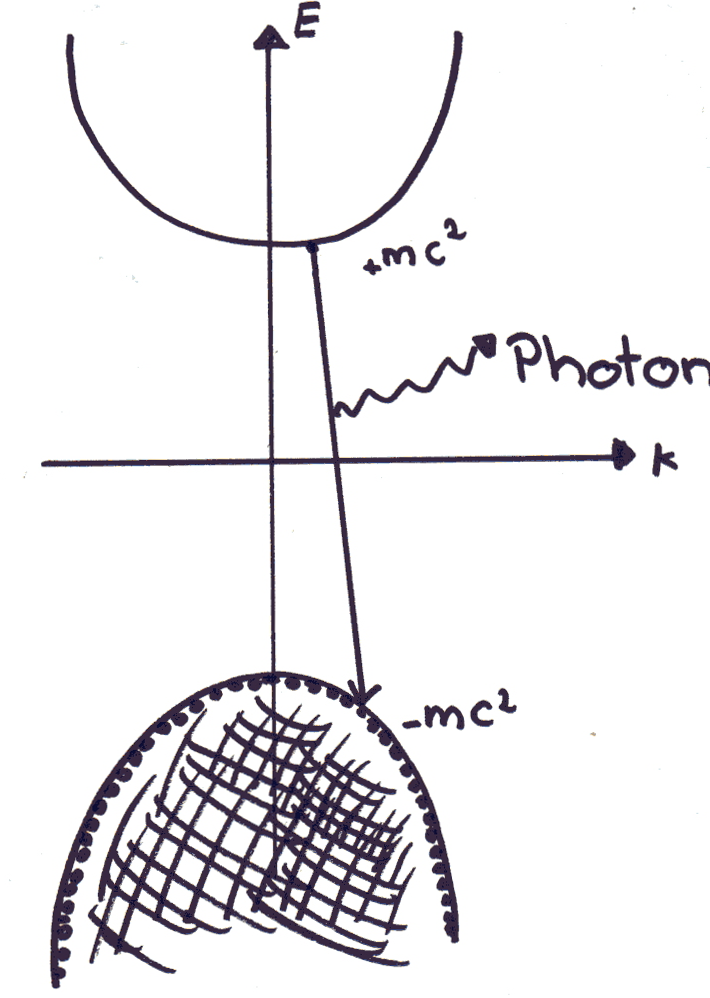
\includegraphics[scale=0.15]{Figs/Pim000114.png}
\end{center}
\end{wrapfigure}
\underline{Ausweg:} Dirac 1930\\
Alle Zustände negativer Energie sind besetzt. Wegen des Pauliverbots sind somit die Zustände negativer Energie für die Elektronen unerreichbar:\\

Der Vakuumzustand besteht aus einem See von unendlich vielen Teilchen negativer Energie, die alle Zustände besetzen.\\
\\
\underline{Anregung des Vakuums:}\\
Ein Elektron aus dem Diracsee wird in einem Zustand positiver Energie angeregt. Zurück bleibt ein \underline{Loch} im Diracsee mit folgenden Eigenschaften:
\begin{itemize}
\item Ladung:  $-q_e = e > 0$
\item Wellenfunktion des ursprünglichen Elektrons
\begin{eqnarray*} 
	v_s(p)e^{ipx} = v_s(p) e^{i(E_pt-\vec p\vec x)}
\end{eqnarray*} 
mit der Energie $-E_p>0$ und dem Impuls$-\vec p$. Ist der Zustand nicht besetzt, so ist der Energieunterschied größer 0. 
\item Spin:  $-s \frac \hbar 2$
\end{itemize}
\underline{Interpretation}\\
Das Loch verhält sich wie ein Teilchen mit der Energie $E$, Impuls $\vec p$, Ladung $+e$ und Spin $s\frac\hbar 2$.\\
$\Longrightarrow$ Antiteilchen (Positron)\\
Das Antiteilchen wurde experimentell nachgewiesen.

Probleme: 
\begin{itemize}
\item In der Diractheorie ist die Energie des Vakuums unendlich, und die Wechselwirkung zwischen den Teilchen wird vernachlässigt.
\item Die Dirac-Theorie dient der Beschreibung von Ein-Teilchen-Systemen. Im Dirac-See existieren aber unendlich viele Löcher. 
\item Es bleibt unklar, was für die Symmetriebrechung sorgt, die dazu führt, dass Elektronen und nicht Positronen unbesetzte Zustände besetzen. 
\end{itemize}

 \newpage
\setcounter{section}{3}
\setcounter{equation}{0}
\thispagestyle{plain} 
\kapitel{Quantenfeldtheorie}{Quantenfeldtheorie}
\thispagestyle{plain} 
\underline{Motivation}
\begin{itemize}
\item relativistische Einteilchenteorie führt zu Widersprüchen.
\item Kerne, Atome, Moleküle, Festkörper bestehen aus großer Anzahl Teilchen
\item Elementarteilchen- und -anregungen können erzeugt oder vernichtet werden
\end{itemize}
\subsection{Teilchensysteme}
\subsubsection{Ein Teilchen}
Wellenfunktion$\qquad \psi(\vec r, t)$\\
Schrödingergleichung \begin{eqnarray*} i\hbar \partial_t \psi = \ham \psi \qquad \ham = T + U\quad U = U(\vec r)\quad T = \frac{\vec p^2}{2m}\end{eqnarray*}
\subsubsection{Zwei identische Teilchen}
Wellenfunktion $\psi(\vec r_1,\vec r_2,)$ hängt nun von beiden Koordinaten ab.\\
Beide Teilchen sind identisch, d.h. wenn wir die beiden Koordinaten vertauschen, darf sich die Physik sich nicht ändern.\\
z.B. Wahrscheinlichkeitsdichte
\begin{eqnarray*}
W(\vec r_1,\vec r_2)\g \left |\psi(\vec r_1,\vec r_2)\ri|^2 = W(\vec r_2,\vec r_1) = \left |\psi(\vec r_2,\vec r_1)\ri|^2\\
\Longrightarrow \psi(\vec r_1,\vec r_2) \g e^{i\varphi} \psi(\vec r_2,\vec r_1)
\end{eqnarray*}
In der Praxis kommen zwei Fälle vor
\begin{eqnarray*}
\psi(\vec r_1, \vec r_2) \g \psi(\vec r_2,\vec r_1) \qquad\qquad \begin{array}c\text{Bosonen (Photon, Phonon)}\\\text{Teilchen mit ganzem Spin}\end{array}\\
-\psi(\vec r_2,\vec r_1) \g \psi(\vec r_1,\vec r_2) \qquad\qquad \begin{array}c \text{Fermionen(Elektron)}\\\text{Teilchen mit halbzahligem Spin}\end{array}
\end{eqnarray*}
Wenn die Teilchen sich jeweils in der Wellenfunktion $\phi_1(\vec r)$ oder $\phi_2(\vec r)$ befinden, so erhalten wir die Zweiteilchenwellenfunktion
\begin{eqnarray*}
\psi_\pm (\vec r_1,\vec r_2) \g \frac 1 {\sqrt{2}} \left[\phi_1(\vec r_1)\phi_2(\vec r_2)\pm\phi_2(\vec r_1)\phi_1(\vec r_2)\ri]\\
\text{ mit  }&+& \text{für Bosonen}\\
\text{und   }&-&\text{für Fermionen}
\end{eqnarray*}
Folge: Pauli-Verbot für zwei Fermionen im gleichen Orbital $\phi_1 = \phi_2$, da sonst gilt:
\begin{eqnarray*} \psi_- = \frac 1 {\sqrt 2}\left[\phi_1(\vec r_1)\phi_1(\vec r_2) - \phi_1(\vec r_2)\phi_1(\vec r_1) \ri] = 0
\end{eqnarray*}
Hamiltonoperator enthält die Einteilchenhamiltonoperatoren und die Zweiteilchenwechselwirkung
\begin{eqnarray*}
\ham_2 \g \sum \limits_{\alpha=1}^2 \ham(\vec r_\alpha, \vec p_\alpha) + V(\vec r_1, \vec r_2)\\
\text{ wobei  }&{}& \ham(\vec r, \vec p) = T(\vec p) + U(\vec r)
\end{eqnarray*}
z.B. Coulomb-Wechselwirkung
\begin{eqnarray*} V(\vec r_1,\vec r_2) =\frac{e^2}{4\pi\varepsilon_0 |\vec r_1-\vec r_2|}\end{eqnarray*}
\subsubsection{Viele Teilchen}
Vereinfachte Schreibweise mit (Anti-) Symmetrisierungsoperator $S_+\ (S_-)$.\\
Dieser macht aus dem Produkt von $n$ Wellenfunktionen die symmetrisierte Form, bei der alle Koordinaten permutiert werden (Bei Fermionen ergibt jede Permutation ein Minuszeichen).\\
Wellenfunktion für $N$ Teilchen ist:
\begin{eqnarray*} \psi_{\{i\}}^\pm \{\vec r_1, \dots,\vec r_N\} = \frac 1 {\sqrt N} S_\pm \left(\phi_{i_1}(\vec r_1), \dots \phi_{i_N}(\vec r_N)\ri)
\end{eqnarray*}
Für Fermionen kann dies als Slater-Determinante  geschrieben werden:
\begin{eqnarray*}
\psi_N^- = \frac 1 {\sqrt N} \left| \begin{array}{cccc}\phi_{i_1}(\vec r_1) & \phi_{i_2}(\vec r_1) & \dots&\phi_{i_N}(\vec r_1)\\ \vdots& {\vdots}&{\ddots}&\vdots\\\phi_{i_1}(\vec r_N) & \phi_{i_2}(\vec r_N)&\dots&\phi_{i_N}(\vec r_N)\end{array}\ri |
\end{eqnarray*}
Hamiltonoperator:
\begin{eqnarray*}
\ham _N = \sum \limits_{\alpha = 1}^N \ham (\vec r_{\alpha}, \vec p_\alpha ) + \frac 1 2 \sum \limits_{\alpha \neq \beta} V(\vec r_\alpha,\vec r_\beta ) \end{eqnarray*}
Für allgemeine Zustände bilden die $\psi_{\{i\}}^\pm$ für alle $\{i\}$ eine Basis im $N$-Teilchen Hilbertraum.

Es gilt in Ket- Schreibweise
\begin{eqnarray*} \left | \psi_N \ro = \sum \limits_{\{i\}} c_{i_1} \dots c_{i_N} S^\pm \left ( \left | i_1 \ro \left | i_2 \ro \dots \left | i_N \ro \ri)
\end{eqnarray*}
Die Zustände können vereinfacht in der linear unabhängigen sogenannten Besetzungszahlbasis dargestellt werden.
Wir wählen für jedem äquivalenten Zustand einen Vertreter aus.
\begin{eqnarray*} \left |n_1,n_2, \dots \ro = \left \{ \begin{array}{rc} S^- \left(\left| i_1 \ro \left | i_2 \ro \dots \left | i_N\ro \ri)&\text{Fermionen} \\ \frac 1 {\sqrt{n_1 \cdot n_2 \dots}} S^+ \left(\left| i_1 \ro \left | i_2 \ro \dots \left | i_N\ro \ri)&\text{Bosonen}\end{array}\ri.
\end{eqnarray*}
$n_i$ gibt an wie vielfach der Zustand $i$ besetzt wird. Für Fermionen gilt $n_i = 0,1$ für Bosonen $n_i = 0,1,2,\dots$\\
Zusammen:
\begin{eqnarray*} N = \sum \limits _i ^\infty n_i\end{eqnarray*}
Besetzungszahlzustände bilden eine vollständige Orthonormalbasis im $N$-Teilchen Hilbertraum.
\begin{eqnarray*}
\lo n_1,n_2,\dots \s n'_1,n'_2,\dots \ro = \delta_{n_1n'_1}\delta_{n_2n'_2}\dots\\
\sum \limits_{n_1 = 0}^{1(\infty)}\sum \limits_{n_2 = 0}^{1(\infty)}\dots \delta_{N_i \sum \limits _i n_i }\s n_1, n_2,\dots\big>\big< n_1,n_2,\dots\s = \mathds 1
\end{eqnarray*}


\subsubsection{Fockraum}
Wir bilden die direkte Summe aller Hilberträume $\hil_n$ mit $N=0,1,2,\dots$
\begin{eqnarray*}
\mathscr F = {\oplus}  _{N = 0}^\infty \hil_N\qquad \text{Fockraum}
\end{eqnarray*}
Die Besetzungszahlbasis ohne Einschränkung ($\sum \limits_i n_i = N$) ist eine VONB im Fockraum, d.h. es gilt
\begin{eqnarray*}
\sum \limits _{n_1 = 0}^{1 (\infty)} \sum \limits _{n_2 = 0}^{1 (\infty)}\dots \s n_1,n_2,\dots\big >\big<n_1,n_2,\dots\s=\mathds 1\qquad\text{für  Fermionen (Bosonen).}
\end{eqnarray*}
$\hil_0$  enthält einen Zustand ohne Teilchen.\\
$\longrightarrow$ Vakuumszustand $\s 0 \big > = \s 0,0,\dots\big >$    \Big($\lo0\s0\ro = 1$\Big)



 \newpage
\thispagestyle{plain} \subsection{Erzeuger und Vernichter}
Um Operatoren im Fockraum in einer teilchenzahlunabhängigen Weise auszudrücken, führen wir sog. Erzeugungs- und Vernichtungsoperatoren ein, die Hilberträume mit verschiedenen Teilchenzahlen verbinden.
\subsubsection{Bosonen:} Erzeugungsoperator erhöht die Besetzungszahl um 1
\begin{eqnarray*}
a_i^\dagger \left | \dots n_i \dots \ro = \sqrt{n_i + 1 } \left | \dots n_i + 1\dots \ro 
\end{eqnarray*}
Der adjungierte Operator erniedrigt Besetzung um 1
\begin{eqnarray*}
a_i \left | \dots n_i \dots \ro = \sqrt {n_i} \left | \dots n_i - 1 \dots \ro
\end{eqnarray*}
Insbesondere gilt für den Vakuumszustand:
\begin{eqnarray*}
a_i \left | 0 \ro = 0\qquad \text{f.a.}\quad i
\end{eqnarray*}
Aus der Definition folgen die Vertauschungsrelationen
\begin{eqnarray*}
\left [ a_i,a_j \ri] = 0  \qquad \left[a_i^\dagger,a_j^\dagger\ri] = 0 \qquad \left[ a_i,a_j^\dagger \ri] = \delta_{i j}
\end{eqnarray*}
\underline{Beweis}
\begin{eqnarray*}
&{}&\left[a_i^\dagger ,a_j^\dagger\ri ] \left | \dots,n_i,\dots,n_j,\dots\ro \qquad i\neq j\\
\g \left(a_i^\dagger a_j^\dagger - a_j^\dagger a_i^\dagger \ri ) \left | \dots, n_i,\dots,n_j,\dots\ro\\
\g \left( \sqrt{n_i+1}\sqrt{n_j+1}-\sqrt{n_j+1}\sqrt{n_i+1}\ri)\left|\dots,n_{i+1},\dots,n_{j+1},\dots\ro\\
\g  0
\end{eqnarray*}
\begin{eqnarray*}
&{}&\left[a_i,a_j^\dagger\ri] \left | \dots ,n_i,\dots,n_j,\dots\ro\\
\g \left(a_i a_j^\dagger - a_j^\dagger a_i\ri ) \left | \dots,n_i,\dots,n_j,\dots\ro\\
&\overset{(i\neq j)} =& \big(\underbrace{\sqrt{n_i}\sqrt{n_j+1} - \sqrt{n_j+1}\sqrt{n_i}}_{=0}\big) \left| \dots,n_{i-1},\dots,n_{j+1},\dots\ro
\end{eqnarray*}
\begin{eqnarray*}
&{}&\left[a_i,a_i^\dagger\ri] \left| \dots,n_i,\dots\ro\\
\g \left (a_ia_i^\dagger - a_i^\dagger a_i\ri) \left |\dots,n_i,\dots\ro\\
\g a_i \sqrt{n_i+1} \left |\dots,n_{i+1},\dots\ro-a_i^\dagger \sqrt{n_i}\left |\dots,n_{i-1},\dots\ro\\
\g (n_{i}+1) \left |\dots,n_i,\dots\ro\ -n_i\left |\dots,n_i,\dots\ro\\
\g \left |\dots,n_i,\dots\ro\qquad\qquad \text{vgl.  }\left[a,a^\dagger \ri]=1\qquad \text{(harm.Oszi.)}
\end{eqnarray*}
Alle Zustände können aus dem Vakuumzustand erzeugt werden:
\begin{eqnarray*}
\left | n_1,n_2,\dots\ro = \frac 1 {\sqrt{n_1\cdot n_2\cdot\dots}}\left(a_1^\dagger\ri)^{n_1}\left(a_2^\dagger\ri)^{n_2}\dots \left | 0 \ro
\end{eqnarray*}
Um die Teilchenzahl festzustellen, konstruiert man den Besetzungszahloperator: $\hat n_i = a_i^\dagger a_i$ mit 
\begin{eqnarray*}
\hat n_i = \left | \dots n_i \dots \ro = a_i^\dagger  a_i \left | \dots n_i \dots \ro = n_i \left | n_i \ro
\end{eqnarray*}
Gesamtteilchenzahloperator $\hat N = \sum \limits_i \hat n_i$
\begin{eqnarray*} \lo N \ro = \lo n_1 \dots \s \hat N \s n_1 \dots \ro = \sum n_i \end{eqnarray*}
Für nicht wechselwirkende Teilchen können wir die Eigenzustände des Hamiltonoperators als Einteilchenzustände benutzen ($\ham_1 \phi_1 = \varepsilon_i \phi_i$).\\
Der Vielteilchen-Hamiltonoperator
\begin{eqnarray*} \wh \ham \g \sum \limits_i \varepsilon _i \hat n_i\\
\lo \ham \ro \g \big< n_1 \dots \s \sum \limits_i \varepsilon_i\hat n_i \s n_1 \dots\big> = \sum \varepsilon_i n_i
\end{eqnarray*}


\subsubsection{Fermionen}
Wegen der Antisymmetrie unter Vertauschung zweier Teilchen muss auf die Reihenfolge der Anwendung fermionscher Operatoren geachtet werden.
\begin{eqnarray*}
S_- \left | i_1,i_2,\dots,i_N\ro \g a_{i_1}^\dagger a_{i_2}^\dagger\dots a_{i_N}^\dagger \left | 0 \ro\\
S_- \left | i_2,i_1,\dots,i_N\ro \g a_{i_2}^\dagger a_{i_1}^\dagger\dots a_{i_N}^\dagger \left | 0 \ro\\
 \g -S_-\left |i_1,i_2,\dots,i_N\ro\\
\Longrightarrow a_{i_1}^\dagger a_{i_2}^\dagger + a_{i_2}^\dagger a_{i_1}^\dagger \g 0\\
\left\{a_{i_1}^\dagger,a_{i_2}^\dagger \ri \} \g 0 \qquad \text{Antikommutator}\\
\text{allg.  }\left\{a_i^\dagger,a_j^\dagger \ri\} \g 0
\end{eqnarray*}
es folgt für $i = j $: 
\begin{eqnarray*} a_i^\dagger a_i^\dagger = \left(a_i^\dagger \ri )^2 = 0\end{eqnarray*}
Alle Zustände können aus dem Vakuum erzeugt werden die Reihenfolge muss einmal festgelegt werden.
\begin{eqnarray*}
\left | n_1,n_2,\dots \ro = \left(a_1 ^\dagger \ri)^{n_1} \left(a_2^\dagger \ri)^{n_2}\dots \left | 0 \ro
\end{eqnarray*}
Für Erzeugungs- und Vernichtungsoperatoren folgt:\\
\begin{eqnarray*}
a_i^\dagger \left | \dots n_i \dots \ro \g \left (1 -n_1 \ri) \underbrace{(-1)^{\sum \limits_{j<i}n_j}}_{=p_i} \left | \dots n_i+1 \dots \ro\\
a_i \left | \dots n_i \dots \ro \g n_i p_i \left | \dots n_i-1 \dots \ro
\end{eqnarray*} 
Beachte: $n_i = 0,1$.
Besetzungszahloperator  $\hat n_i = a_i^\dagger a_i$
\begin{eqnarray*} \hat n_i \left | \dots n_i \dots \ro = n_i \left | \dots n_i \dots \ro
\end{eqnarray*}
Algebra folgt zum Beispiel aus:
\begin{eqnarray*} &{}& \left \{a_i,a_i^\dagger \ri \} \left | \dots n_i \dots\ro\\
\g \left(a_ia_i^\dagger + a_i^\dagger a_i \ri) \left | \dots n_i\dots\ro\\
\g a_i(1 -n_i)p_i \left | \dots n_i+1\dots\ro + a_i^\dagger n_ip_i \left |\dots n_i-1\dots\ro\\
\g \left [(n_i+1)(1-n_i) + n_i(2-n_i)\ri] \left | \dots n_i\dots\ro\\
&\overset{n^2 = n}{=}& \left | \dots n_i \dots \ro\\
\Longrightarrow \left\{a_i,a_i^\dagger \ri \} \g 1
\end{eqnarray*}
Es gilt für Fermionen
\begin{eqnarray*}
\boxed{\{a_i,a_j\} = 0 \qquad \{a_i^\dagger,a_j^\dagger\} = 0 \qquad \{a_i,a_j^\dagger\} =\delta _{ij}}
\end{eqnarray*}
 \newpage
\thispagestyle{plain} \subsection{Operatoren in zweiter Quantisierung}
\subsubsection{Einteilchenoperator}
\begin{eqnarray*}
T = \sum \limits_{\alpha = 1}^N T_\alpha \qquad \left(\text{z.B. }T_\alpha = \frac{p_\alpha^2}{2m}\ri)
\end{eqnarray*}
In Basis $\left|i\ro$ gilt:
\begin{eqnarray*}
T_{ij} \g \lo i \s T \s j \ro\\
\text{und } t \g \sum \limits_{ij}T_{ij} \left | i \ro\lo j\ri|
\end{eqnarray*}
Zusammen
\begin{eqnarray*}
T = \sum \limits _{ij } T_{ij} \underbrace{\sum \limits_{\alpha = 1}^N \left |i \ro_\alpha\lo j\right |_\alpha }_{O}
\end{eqnarray*}
Die Wirkung von $O$ auf einen Zustand ist es ein Teilchen im Zustand $\left |j\ro$ durch eines im Zustand $\left |i \ro$ zu ersetzen. Die Wirkung ist identisch zum Operator $a_i^\dagger a_i$, d.h. es gilt 
\begin{eqnarray*} a_i^\dagger a_i = \sum \limits_{\alpha = 1}^N \left |i\ro_\alpha\lo j\ri| _\alpha.\end{eqnarray*}
Wir erhalten
\begin{eqnarray*}
	\boxed{T = \sum \limits_{i j} T_{i j} a_i^\dagger a_j}
\end{eqnarray*}
Allgemeine Form eines Einteilchenoperators unabhängig von der Teilchenzahl!

\subsubsection{Zweiteilchenoperaor}
\begin{eqnarray*}
V &=& \frac 1 2 \sum_{\alpha\neq \beta} V (\vec r_\alpha, \vec r_\beta)
\\
&=& \frac 1 2 \sum_{ijkm}\sum_{\alpha \neq \beta} \underbrace{\,_{\alpha}\bra{i}\!\,_{\beta}\bra{j}V\ket{k}_{\alpha}\ket{m}_{\beta}}_{V_{ijkm}} \quad \ket{i}_{\alpha}\ket{j}_{\beta}\,_{\alpha}\bra{k}\!\,_{\beta}\bra{m}
\\
&=& a_i^\dagger a_j^\dagger a_m a_k\\
\end{eqnarray*}
wobei gilt
\begin{eqnarray*}
\sum_{\alpha\neq \beta} \ket{i}_{\alpha}\ket{j}_{\beta}\,_{\alpha}\bra{k}\!\,_{\beta}\bra{m} &=&
\sum_{\alpha \neq \beta} \underbrace{\ket{i}_{\alpha}\,_{\alpha}\bra{k}\ket{j}_{\beta}\,_{\beta}\bra{m}}_{a_i^\dagger a_k \quad a_j^\dagger a_m} - \underbrace{\braket{k}{j}}_{\delta_{kj}}\quad \sum_{\alpha} \underbrace{\ket{i}_{\alpha}\,_{\alpha}\bra{m}}_{a_i^\dagger a_m}
\end{eqnarray*}
Allgemeiner Zweiteilchenoperator:
\begin{eqnarray*} \boxed{ V = \frac 1 2 \sum \limits_{ijkm} V_{ijkm} a_i^\dagger a_j^\dagger a_m a_k}\end{eqnarray*}
Matrixelement:
\begin{eqnarray*} V_{ijkm} = \int d^3 x_1 d^3x_2\quad \phi_i^* (\vec x_1) \phi^* _j(\vec x_2) V(\vec x_1,\vec x_2) \phi_k(\vec x_1)\phi_m(\vec x_2)
\end{eqnarray*}


\subsubsection{Hamiltonoperator}
\begin{eqnarray*}
\wh \ham = \sum_{ij} T_{ij} a_i^\dagger a_j + \sum \limits_{ijkm} V_{ijkm} a_i^\dagger a_j^\dagger a_m a_k
\end{eqnarray*}
Der erste Term beschreibt die kinetische Energie in der Eigenbasis von $\ham_1$, der zweite Term die Wechselwirkung zwischen jeweils zwei Teilchen. 

Der Hamiltonoperator hat folgende Eigenschaften: 
\begin{itemize}
\item Operator im Fockraum unabhängig von Teilchenzahl
\item für Bosonen und Fermionen identisch
\item aufgrund des nicht quadratischen Terms $\sim a^\dagger a^\dagger a a$ im Allgemeinen nicht lösbar
\end{itemize}
 \newpage
\thispagestyle{plain} \subsection{Feldoperatoren}
\subsubsection{Basiswechsel}
Der Wechsel von einer Basis $\{\ket{i}\}$ in eine Basis $\{\ket{\lambda}\}$ erfolgt wie bekannt durch:
\begin{eqnarray*}
\ket{\lambda} &=& \sum_i \ket{i}\braket{i}{\lambda}
\end{eqnarray*}
Operatoren transformieren sich wie folgt: 
\begin{eqnarray*}
a_\lambda^\dagger &=& \sum_i \braket{i}{\lambda} a_i^\dagger
\\
a_\lambda &=& \sum_i \braket{\lambda}{i} a_i
\end{eqnarray*}
Die Vertauschungsrelationen bleiben unter Basistransformationen erhalten.
\begin{eqnarray*}
\left[ a_\lambda , a_{\lambda'}^\dagger \ri ] _\pm \g \sum \limits_{i j} \underbrace{ \left[ a_i, a_j^\dagger \ri ]_\pm}_{\delta_{i j}} \braket{\lambda}{i}\braket{j}{\lambda'}
\\
&=& \bra{\lambda} \underbrace{\sum_i  \ket{i}\bra{i}}_{\1}\!\!\!\,\,{\lambda'}\rangle = \braket{\lambda}{\lambda'} = \delta_{\lambda \lambda '}
\end{eqnarray*}


\subsubsection{Ortsdarstellung}
Für die Ortsbasis gilt $\phi_i(\vec r) = \lo \vec r \s i \ro$\\
Die entsprechenden Erzeugungs- und Vernichtungsoperatoren heißen {\bf Feldoperatoren}.
\begin{eqnarray*}
\boxed{\wh\Psi(\vec r) = \sum \limits_ i \phi _i(\vec r) a_i \qquad
\wh\Psi^\dagger(\vec r) = \sum \limits_ i \phi^* _i(\vec r) a_i^\dagger}
\end{eqnarray*}
Dabei vernichtet $\wh\Psi(\vec r)$ ein Teilchen am Ort $\vec{r}$ und $\wh\Psi^\dagger(\vec r)$ erzeugt eines.

Die Vertauschungsrelationen
\begin{eqnarray*}
\left[\wh\Psi(\vec r),\wh\Psi(\vec r\,{'})\ri]_\pm = \left[\wh\Psi^\dagger(\vec r),\wh\Psi^\dagger(\vec r\,{'})\ri]_\pm &=& 0 
\\
\left[\wh\Psi^(\vec r),\wh\Psi^\dagger (\vec r\,{'})\ri]_\pm &=& \delta(\vec r - \vec r\,{'})
\end{eqnarray*}
Beispiele für Operatoren:
Kinetische Energie:
\begin{eqnarray*} \hat T = \int \mathrm{d}^3r \ \ \wh\Psi^\dagger (\vec r) \left ( \frac {-\hbar^2 \Delta}{2 m}\ri) \wh\Psi(\vec r)
\end{eqnarray*}
Potentielle Energie:
\begin{eqnarray*} \hat U = \int \mathrm{d}^3r \ \ U(\vec r) \wh\Psi^ \dagger (\vec r)\wh\Psi(\vec r)
\end{eqnarray*}
Teilchendichte:
\begin{eqnarray*}
\hat n (\vec r) = \sum \limits _\alpha \delta(\vec r - \vec r_\alpha) = \wh\Psi^\dagger (\vec r)\wh\Psi(\vec r)
\end{eqnarray*}
Zweiteilchenoperator:
\begin{eqnarray*}
\hat V = \int \mathrm{d}^3r \mathrm{d}^3r'\ \ \wh\Psi^\dagger(\vec r)\wh\Psi^\dagger (\vec r\,{'}) V(\vec r, \vec r\,{'}) \wh\Psi(\vec r\,{'})\wh\Psi(\vec r)
\end{eqnarray*}
Vielteilchenhamiltonoperator;
\begin{eqnarray*} \wh \ham = \hat T + \hat V + \hat U\end{eqnarray*}

\subsubsection{Bewegungsgleichung}
Die Heisenberg-Gleichung für Felder
\begin{eqnarray*}
i\hbar \partial_t \wh\Psi(\vec r, t) \g \left[ \wh\Psi(\vec r, t), \wh \ham\ri]
\\
\cdots &=& \left ( - \frac {\hbar^2}{2 m} \Delta + U(\vec r)\ri) \wh\Psi (\vec r, t) + \frac 1 2 \int \mathrm{d}^3r' \wh\Psi^\dagger (\vec r\,{'}, t) V(\vec r, \vec r\,{'}) \wh\Psi(\vec r\,{'}, t)\wh\Psi(\vec r, t)
\end{eqnarray*}
\begin{itemize}
\item Für $V=0$ erinnert die Bewegungsgleichung an die Einteilchen- Schrödingergleichung.\\
$\longrightarrow$ Bekannte Methoden können zur Lösung genutzt werden.
\item $V\neq 0$ (,, many-body-problem'')\\
Die Gleichung ist \underline{nicht linear} in den Feldoperatoren (außerdem integro-differential).
\item Stromdichte: Aus den Bewegungsgleichungen für $\wh\Psi$ und $\wh\Psi^\dagger$ folgt:
\begin{eqnarray*}
\hat n (\vec r, t) \g \divergenz  \hat{\vec  j}\\
\text{mit }\hat{\vec j} \g \frac {i \hbar}{2 m} \left( \wh\Psi^\dagger \nabla \wh\Psi - \big(\nabla \wh\Psi^\dagger\big) \wh\Psi\ri)
\end{eqnarray*}
\end{itemize}

\subsubsection{Impulsdarstellung / Feynmandiagramme}
Impulsdarstellung, insbesondere für translationsinvariante Systeme.
\begin{eqnarray*}
\phi_{\vec k} (\vec r) = \frac 1 {\sqrt v} e^{i \vec k\vec r}
\end{eqnarray*}
Algebra für $a_{\vec k},a^\dagger_{\vec k}$
\begin{eqnarray*}
\left [ a_{\vec k}, a_{\vec k'}\ri ] \g 0\\
\left [ a_{\vec k}, a_{\vec k'}^\dagger\ri ] \g \delta_{\vec k,\vec k'}\\
\end{eqnarray*}
Hamiltonoperator
\begin{eqnarray*}
\ham &=& \sum \limits_{\vec k} \frac{\hbar^2\vec k^2}{2 m} a^\dagger_{\vec k} a_{\vec k} + \sum \limits_{\vec k,\vec k'} U_{\vec k-\vec k'}a_{\vec k}^\dagger a_{\vec k'} + \frac 1 {2V} \sum \limits_{\vec k\vec k',\vec q} a_{\vec k+\vec q}^\dagger a_{\vec k'-\vec q}^\dagger V_{ \vec q} a_{\vec k'}a_{\vec k}
\end{eqnarray*}
Die Matrixelemente sind
\begin{eqnarray*}
U_{\vec k-\vec k'} \g \int \mathrm{d}^3r\quad U(\vec r) e^{-i(\vec k-\vec k') \vec r}\\
V_{\vec q} \g \int \mathrm{d}^3r\quad V(\vec r) e^{-i\vec q \vec r} 
\end{eqnarray*}
Die Potential- und Wechselwirkungs-Terme können grafisch in sogenannten Feynman-Diagramme repräsentiert werden.
\begin{center}
	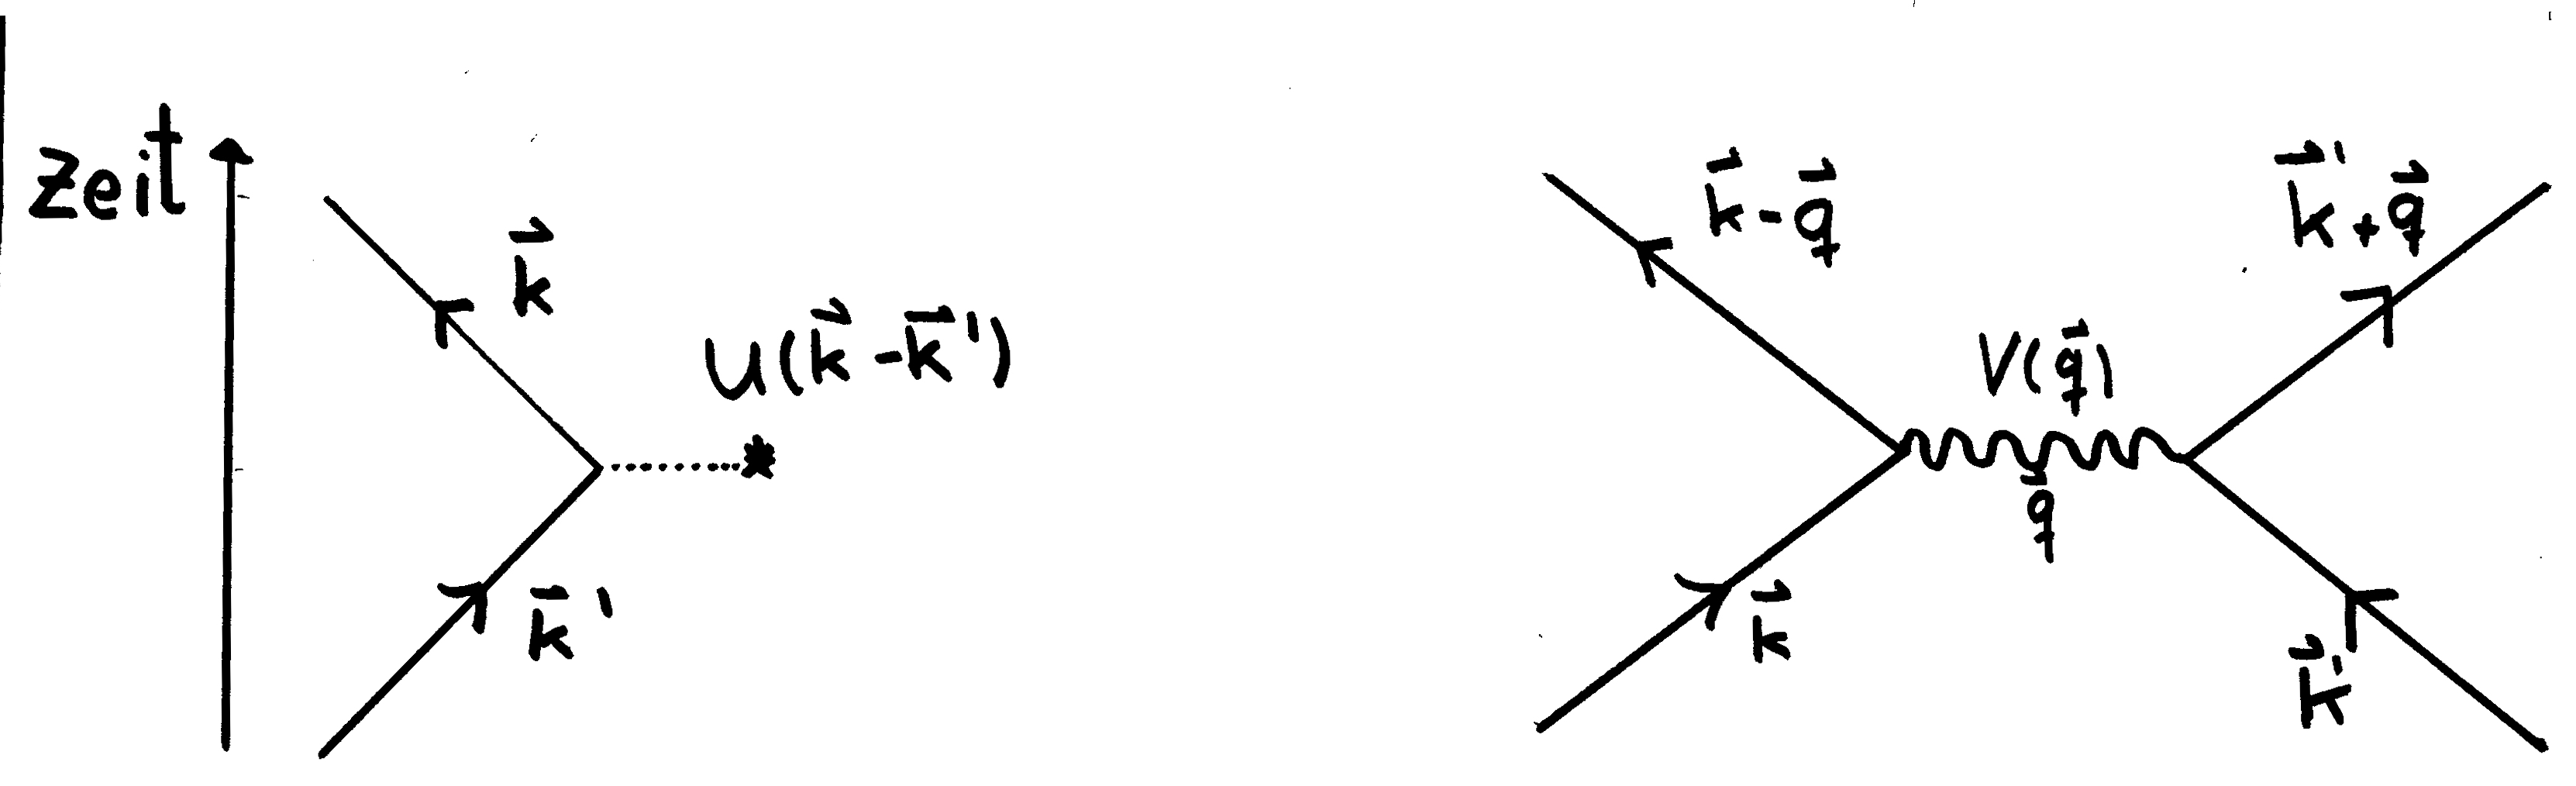
\includegraphics[scale=0.10]{Figs/Pim000113.png}
\end{center}
\subsubsection{Spin}
Feldoperatoren erhalten zusätzlichen Index $\sigma$ für den Spin. Es gilt
\begin{eqnarray*}\left[ \wh\Psi_\sigma(\vec r),\wh\Psi_{\sigma '}^\dagger(\vec r\,{'})\ri]_\pm = \delta_{\sigma\sigma'} \delta(\vec r-\vec r\,{'})
\end{eqnarray*}
Einteilchenoperatoren enthalten Summen über Spin. Zum Beispiel
\begin{eqnarray*}
\hat n (\vec r) = \sum_\sigma \wh\Psi^\dagger_{\sigma}(\vec r) \wh\Psi_\sigma (\vec r) = \sum_\sigma \hat n_\sigma (\vec r)
\end{eqnarray*}
Hamiltonoperator
\begin{eqnarray*}
\wh \ham \g \sum_\sigma \int \mathrm{d}^3r \wh\Psi_\sigma^\dagger(\vec r) \left( -\frac{\hbar^2 \Delta}{2m} + U(\vec r)\ri) \wh\Psi_\sigma(\vec r)\\
&{}&\quad + \sum_{\sigma,\sigma'} \int \mathrm{d}^3r \mathrm{d}^3r'\ \wh\Psi_\sigma^\dagger(\vec r)\wh\Psi_{\sigma'}^\dagger(\vec r\,{'}) V(\vec r, \vec r\,{'}) \wh\Psi_{\sigma'}(\vec r\,{'}) \wh\Psi_{\sigma}(\vec r)
\end{eqnarray*}
{Bemerkung:}\\
Die Wechselwirkung ist unterschiedlich zwischen Teilchen mit gleichem und ungleichem Spin.\\ \\
\underline{Spindichteoperator}
\begin{eqnarray*}
\vec S(\vec r) = \sum \limits_\alpha \delta(\vec r-\vec r\,{'}_\alpha) \vec s_\alpha
\end{eqnarray*}
Für Spin-$\frac 1 2$ Teilchen$\qquad S = \frac \hbar 2 (\sigma_x,\sigma_y,\sigma_z)$\\
In 2. Quantisierung
\begin{eqnarray*} \vec S(\vec r) = \frac \hbar 2  \sum_{\sigma \sigma'} \wh\Psi_\sigma^\dagger (\vec r ) \vec \sigma_{\sigma \sigma'}\wh\Psi_{\sigma'}(\vec r)
\end{eqnarray*}
Gesamtspin:
\begin{eqnarray*}
\vec S = \int \mathrm{d}^3r \ \vec s(\vec r)\end{eqnarray*}
Erfüllt Drehimpulsalgebra
\begin{eqnarray*}
\left [ S_i,S_j\ri] = i\hbar \varepsilon_{ijk}S_k
\end{eqnarray*}


 \newpage
\thispagestyle{plain} \subsection{Feldquantisierung der Diractheorie}
\subsubsection{Erzeugungs- und Vernichtungsoperatoren}
Einteilchenlösungen:
\begin{eqnarray*}
\psi^\pm_{\sigma k}(x) \g \sqrt{\frac{m}{VE_k}} u_\sigma^\pm(k) \ e^{\mp i k x}\\
\text{mit  }u_\sigma^+(k) \g u_\sigma(k) = \sqrt{\frac{E+m}{2 m}} \left(\begin{array}c \chi_\sigma\\\frac{\vec \sigma \vec k}{E+m}\chi_\sigma\end{array}\ri)\\
u_\sigma^-(k) \g v_\sigma(k) = \sqrt{\frac{E+m}{2 m}} \left(\begin{array}c \frac{\vec \sigma \vec k}{E+m} \chi_\sigma\\\chi_\sigma\end{array}\ri)
\end{eqnarray*}
Es gilt mit adjungierten Spinoren
\begin{eqnarray*} \bar u_\sigma^\alpha \g u_\sigma^{\alpha \dagger}\gamma^0\qquad \alpha = \pm\\
\bar u_\sigma^\alpha u_{\sigma'}^\beta \g\alpha \delta_{\alpha \beta }\delta_{\sigma\sigma'}
\end{eqnarray*}

\underline{Definition}
\begin{center}
	\begin{tabular}{|l l|l|}\hline
		$b_{\sigma k}^\dagger$& erzeugt & Elektronen \\ \cline{1-2}
		$b_{\sigma k}$ & vernichtet & \\\hline
		$d_{\sigma k}^\dagger$ & erzeugt & Positronen \\ \cline{1-2}
		$d_{\sigma k}$ & vernichtet&\\\hline
	\end{tabular}
\end{center}
Spinor $u^\pm_\sigma (\vec k)$ mit Energie $ E = k^0 = \sqrt{k^2 + m^2} > 0 $ und Spin  $ \sigma$ . 
Da Elektronen/Positronen Fermionen sind, führen wir Antivertauschungsrelationen ein:
\begin{eqnarray*}
\left \{b_{\sigma k}, b^+ _{\sigma'k'}\ri \} = \delta_{\sigma\sigma'}\delta_{k k'}% = \left \{\delta_{\delta k}, \delta^\dagger_{\sigma' k'}\ri\}
\qquad \qquad \{d_{\sigma k},d_{\sigma' k'}^+ \} = \delta_{\sigma \sigma'}\delta_{k k'}
\end{eqnarray*}
alle anderen verschwinden.
\subsubsection{Feldoperatoren}
Wir entwickeln die Feldoperatoren nach einem \underline{vollständigen} Satz von Lösungen.
\begin{eqnarray*}
\wh\Psi(x) = \sum_{\sigma k } \underbrace{\wh\Psi^+_{\sigma k}(x)b_{\sigma k}}_{\text{nur für Elektronen}} + \underbrace{\wh\Psi^-_{\sigma k}(x) d_{\alpha k }^\dagger(x) }_{\text{wegen Vollständigkeit}}
\end{eqnarray*}
Der adjungierte Feldoperator
\begin{eqnarray*}
\bar{\wh\Psi}(x) = \wh\Psi^\dagger(x) \gamma^0 = \sum_{\sigma k}\bar{\wh\Psi}^+_{\sigma k}(x) b_{\sigma k}^\dagger + \bar{\wh\Psi}_{\sigma k}^-(x) d_{\sigma k}
\end{eqnarray*}
Die Feldoperatoren erfüllen komplizierte Vertauschungsrelationen, da die Kausalität (welche sich mit Lichtgeschwindigkeit ausbreitet) gewahrt bleiben muss. Man findet jedoch für gleiche Zeiten (also beispielsweise im nichtrelativistischen Grenzfall) folgende Vertauschungsrelationen: 
\begin{eqnarray*}
\left\{\wh\Psi_\alpha(t,\vec x), \wh\Psi_\beta^\dagger(t,\vec x)\ri\} = \delta_{\alpha\beta}\delta(\vec x-\vec x')
\end{eqnarray*}
d.h. $\wh\Psi$ und $\wh\Psi$ erfüllen die für fermionische Feldoperatoren geforderten Vertauschungsrelationen.

\underline{Spin-Statistik-Theorem} 
Teilchen mit ganzzahligem/halbzahligem Spin sind Bosonen/Fermionen. Ursache ist, dass die entsprechenden Feldoperatoren für raumartige Abstände vertauschen/antivertauschen müssen.

\subsubsection{Hamiltonoperator}
Der Vierer-Impulsoperator ist
\begin{eqnarray*}
\hat p^\mu &=& \hbar \int d^3x \ \bar{\wh\Psi}(x) (i\dell^\mu \gamma_0) \wh\Psi(x)\\
&\vdots&\\
&=& \hbar\sum_{ k \sigma} k^\mu \left( \hat b^\dagger_{\sigma k }\hat b_{\sigma k} - \hat d_{\sigma k}\hat d^\dagger _{\sigma k}\ri ).
\end{eqnarray*}
Den Hamiltonoperator erhalten wir als die 0-Komponente des Vierer-Impulsoperators. 
\begin{eqnarray*}
\wh\ham &=& \hat p^0 = \sum_{k \sigma} E_{k}\left(\hat b^\dagger_{\sigma k} \hat b_{\sigma k} - \hat d_{\sigma k}\hat d^\dagger _{\sigma k}\ri)
\\
&=& \sum_{k\sigma} E_{k}\big(\underbrace{\hat b^\dagger_{\sigma k }\hat b_{\sigma k}}_{=\hat n^+_{\sigma k}} + \underbrace{\hat d_{\sigma k }^\dagger\hat d_{\sigma k}}_{=\hat n^-_{\sigma k}} -\1 \big) \qquad  \text{mit: } E_k=\hbar k^0=\sqrt{m^2c^4+c^2\hbar^2 \vec{k}^2}
\end{eqnarray*}
Für die Umformung wurde dabei die Antivertauschungsrelation: $\hat d \hat d^\dagger = \1 -\hat d^\dagger\hat d$

Die $\hat n_{k\sigma}$ sind Teilchenzahloperatoren für den Zustand $k\sigma$. Es gilt: $(\hat n_{\sigma k}^\alpha)^2 = \hat n_{\sigma k}^\alpha$, damit hat $n_{\sigma k}^\alpha$ die Eigenwerte 0 und 1. 

Damit ist die Energie immer positiv, da sowohl die Elektronen als auch die Positronen einen positiven Energiebeitrag liefern.

Der letzte Term liefert eine (unendliche) Nullpunktsenergie selbst im Vakuumszustand.

Wir subtrahieren diesen Term vom Hamiltonoperator, um zur physikalischen Observablen Energie zu kommen.
\begin{eqnarray*}
\wh\ham_{\text{neu}} \g \sum \limits_{\sigma k} E_{k} \left (\hat b_{\sigma k}^\dagger \hat b_{\sigma k}+\hat d_{\sigma k}^\dagger\hat d_{\sigma k}\ri)\\
\hat\vec p_{\text{neu}} \g \sum \limits_{\sigma k}\hbar \vec k \left(\hat b_{\sigma k}^\dagger \hat b_{\sigma k} + \hat d_{\sigma k}^\dagger \hat d_{\sigma k}\ri)
\end{eqnarray*}
Der Ladungoperator $\hat Q$ entspricht der 0-Komponte der Viererstromdichte $\hat j^\mu$
\begin{eqnarray*}
\hat Q &=& -e \int \mathrm{d}^3x\; \bar{\wh\Psi}\gamma_0\wh\Psi = j^0 = \dots = -e \sum \limits_{\sigma k}\left(\hat b_{\sigma k}^\dagger \hat b_{\sigma k}-\hat d_{\sigma k}^\dagger \hat d_{\sigma k}\ri) 
\\
\Rightarrow\quad \langle\hat Q\rangle &=& \bra{\psi}{\hat Q}\ket{\psi} =  \Bigg{\{}\!\!\begin{array}{ll} \bra{0}\hat b_{k\sigma} \;\hat Q\; \hat b_{k\sigma}^\dagger\ket{0} & = -e  \\ \bra{0}\hat d_{k\sigma} \;\hat Q\; \hat d_{k\sigma}^\dagger\ket{0} & = +e  \end{array}
\end{eqnarray*}
Damit erzeugt $\hat b^\dagger_{k\sigma}$ Elektronen mit negativer Ladung $-e$ und $\hat d^\dagger_{k\sigma}$ Positronen mit positiver Ladung $+e$. 




 \newpage
\thispagestyle{plain} \subsection{Quantisierung des Strahlungsfeldes}
\subsubsection{Normalmoden, Photonen}
Lagrangefunktion des freien Feldes
\begin{eqnarray*}\Lr \g -\frac 1 {4\mu_0} F_{\mu\nu}F^{\mu\nu}\qquad\qquad F^{\mu\nu} = \partial^{\mu}A^{\nu}- \partial^{\nu}A^{\mu}\\
\g \frac 1 {2 \mu_0}\left(\frac 1 {c^2}\vec E^2 - \vec B^2\ri) = \frac 1 {2 \mu_0}\left(\frac 1 {c^2}\dot{\vec A}^2- (\rot\vec A)^2 \ri)
\end{eqnarray*}
Die Coulombeichung $\dell_i A^i = 0$ kann durch $A^0=0$ gelöst werden. Es ergibt sich folgende Hamiltonfunktion: 
\begin{eqnarray*}
\ham \g -\frac{\partial \Lr}{\partial \dot A^i}\dot A^i-\Lr =\frac 1 {2\mu_0}\left(\frac 1 {c^2}\vec E^2+\vec B^2\ri)
\end{eqnarray*}
Freie Lösungen bestimmt durch Wellengleichung
\begin{eqnarray*}
	\Box \vec A = 0\qquad (\text{ mit }\divergenz \vec A = 0) 
\end{eqnarray*}
Allgemeine Lösung: Zerlegung nach Normalmoden
\begin{eqnarray*}
A^\mu \g \sum \limits_{\vec k,\lambda=1 ,2} \frac 1 {\sqrt{2 |\vec k|V}}\left(e^{-ikx} \varepsilon ^\mu_{\vec k,\lambda} a_{\vec k,\lambda} + e^{ikx}\varepsilon^{\mu *}_{\vec k,\lambda} a^\dagger_{\vec k,\lambda}\ri)\\
\text{mit }&{}&k_0 = |\vec k|\qquad \vec k\vec \varepsilon_{\vec k,\lambda} = 0\qquad \varepsilon^0_{\vec k,\lambda} = 0\\
&{}&\vec \varepsilon_{\vec k,\lambda} \cdot \vec\varepsilon_{k,\lambda'} = \delta_{\lambda,\lambda'}
\end{eqnarray*}
Wir quantisieren:\\
$a_{\vec k\lambda}$ vernichtet Photon mit $\vec k, \lambda$\\
$a_{\vec k\lambda}^\dagger$ erzeugt Photon mit $\vec k, \lambda$\\ \\
Hamiltonoperator:
\begin{eqnarray*}
H = \int d^3 r\ham = \dots = \sum_{\vec k, \lambda} \frac{c\hbar|\vec k|}2 \left(a^\dagger_{\vec k \lambda}a_{\vec k \lambda}+a_{\vec k \lambda}a_{\vec k \lambda}^\dagger \ri)
\end{eqnarray*}
Mit bosonischen Vertauschungsrelationen gilt: $aa^\dagger = 1 + a^\dagger a $ und damit
\begin{eqnarray*} 
	H = \sum \limits_{\vec k \lambda}\hbar \omega_{\vec k}\left(a_{\vec k \lambda}^\dagger a_{\vec k \lambda}+\frac 1 2\ri)
\end{eqnarray*}
Das elektromagnetische Feld ist in quantisierter Form äquivalent zu Normalmoden harmonischer Oszillatoren (die Amplitude entspricht gerade den Feldern).

\subsubsection{Feldoperatoren}
\begin{eqnarray*}
	A^{\mu}_{\lambda k}(x)&=& \varepsilon_{\lambda}^{\mu} \phi_{\vec{k}}(x) \left( e^{-i\omega t} a_{k\lambda} +e^{i\omega t} a^\dagger_{k\lambda} \right)
\\
\Rightarrow \vec E &=& -\dot{\vec A} = -i\omega \varepsilon_{\lambda}\phi_k(x) \left( e^{-i\omega t} a_{k\lambda} +e^{i\omega t} a^\dagger_{k\lambda} \right)
\end{eqnarray*}
\begin{itemize}
\item Feldoperatoren sind hermitesch $\vec E^\dagger = \vec E, \ \vec A^\dagger = \vec A$ und sind daher physikalische Observablen und müssen somit Erzeuger $a^\dagger$ und Vernichter $a$ enthalten.
\begin{eqnarray*}
\left [E^i(\vec r, t),E^j(\vec r',t)\ri] \g 0\\
\left[E^i(\vec r, t), B^j(\vec r, t)\ri] \g i\varepsilon_{ijk}\partial_k\delta(\vec r-\vec r')
\end{eqnarray*}
\item Damit verhalten sich die Feldoperatoren $\vec{E}$ und $\vec{B}$ wie Impuls und Amplitude eines quantenmechanischen harmonischen Oszillators. 
\item Die Fockzustände $\ket{n}$ sind keine Eigenzustände von $\vec{E}$ und $\vec{B}$ und es gibt Fluktuationen (Unschärfen) selbst im Vakuum: 
\begin{eqnarray*}
	\bracket{0}{(\hat a+\hat a^\dagger)}{0}&=&0
	\\
	\bracket{0}{(\hat a+\hat a^\dagger)}{0}&\neq&0
\end{eqnarray*}
\end{itemize}


\subsubsection{Strahlungsübergänge, QED}
Die Kopplung vom elektromagnetischen Feld an Elektronen erfolgt nach dem Prinzip der minimalen Kopplung wie folgt: 
\begin{eqnarray*}
&& \vec p \to \vec p-e\vec A
\\
\Rightarrow& \wh\ham =& \wh\ham_{el} + \wh\ham_{el-ph} + \wh\ham_{ph}
\\
&=& \sum_\sigma \int \mathrm{d}^3r \; \hat{\Psi}_\sigma^\dagger(\vec r) \left(\frac{1}{2m} \left(\hat{\vec{p}}-e\hat{\vec A}(\vec r)\ri)^2 + e\phi(\vec r)\ri) \hat{\Phi}_\sigma(\vec r) + H_{ph}(\hat{\vec{A}})
\\
& \wh\ham_{ph} =& \sum_{\vec k \lambda}\hbar \omega_{\vec k} \hat{a}^\dagger_{\vec k \lambda}\hat{a}_{\vec k \lambda}
\\
& \wh\ham_{el-ph} =& -\frac 1 m \sum_\sigma \int\mathrm{d}^3 r\; \hat{ \Psi}_\sigma^\dagger(\vec r) \hat{\vec A}(\vec{r})\hat{\vec{p}} \hat{\Psi}_\sigma(\vec{r}) + \mathcal{O}(\vec A^2)
\end{eqnarray*}
Strahlungsübergänge folgen in zeitabhängiger Störungstheorie in $\wh\ham_{el-ph}$.
\begin{eqnarray*}
\Gamma_{i-f} = \frac{2 \pi}\hbar \delta(E_f-E_i) |\bra{f}\wh\ham_{el-ph}\ket{i}|^2
\end{eqnarray*}
Hierbei ist $\ket{i/f}=\ket{\psi_{i/f}}_{el}\otimes \ket{\psi_{i/f}}_{ph}$, das heißt es müssen Übergänge der Elektronen und Photonen beachtet werden.

Im klassischen Fall ergibt sich nach Fermis Goldener-Regel (Kapitel 1.2) die Übergangsrate $\Gamma=\dot{P}_{if}$ zu: 
\begin{eqnarray*}
\Gamma^{\text{abs / em}}\propto |\vec{E}_{\omega}|^2\delta(\varepsilon_f-\varepsilon_i \pm \hbar \omega)\end{eqnarray*}
Wobei $|\vec E_{\omega}|^2\propto n_{\omega}$ die Feldenergie ist, welche der Besetzung entspricht. 

In der Quanten Elektro Dynamik ergibt sich die Übergangsrate hingegen wie folgt: 
\begin{eqnarray*}
\bracket{\psi_i}{ (\hat{a}+\hat{a}^\dagger)}{\psi_f} &=&  \bracket{n\pm1}{(\hat{a}+\hat{a}^\dagger)}{n} = \bra{n\pm1}\big(\sqrt{n} \ket{n-1}+ \sqrt{n+1} \ket{n+1}\big)
\\
&=& \Bigg \{ \begin{array}{llc} \sqrt{n} & \text{für Absorption} & (-) \\ \sqrt{n+1} & \text{für Emission}& (+) \end{array}
\\
\Rightarrow\quad \Gamma &\propto& \Bigg \{ \begin{array}{ll} n &\text{für Absorption}\\ n+1 &\text{für stimulierte und spontane Emission }\end{array}
\end{eqnarray*}
\begin{itemize}
\item Absorption und stimulierte Emission ergeben klassische Raten $\propto n\propto |\vec{E}|^2$
\item Spontane Emission ($n=0$) ins Vakuum erfolgt ohne äußeres Feld, verursacht durch sogenannte \underline{Vakuumsfluktuation} und ist eine reine Folgerung aus der QED. 
\end{itemize}


\subsubsection{Der Casimir-Effekt}
Bisher haben wir die Vakuumenergie vernachlässigt, weil sie nicht beobachtbar ist. Vakuumsfluktuationen der Feldamplituden sind aber nach der QED vorhanden.

Dies Vakuumenergie hängt von den Randbedingungen ab. Damit sollte sie messbar sein. Wir betrachten als Beispiel zwei leitende Platten im Abstand $a$. Die Moden sind dann gegeben als: 
\begin{eqnarray*}
\omega(\vec k_\parallel , n) = c \sqrt{|k_\parallel|^2 + \left(\frac{\pi n }a\ri)^2}\qquad n = 1,2,\dots
\end{eqnarray*}
Wegen der Randbedingungen sei $E_\perp = 0$ auf den Platten. Damit ergibt sich eine unterschiedliche Energie im Vakuumzustand mit Platten $E$ und ohne die Platten $E_0$: 
\begin{eqnarray*}
E = \sum_{\vec k \lambda}\frac 1 2 \hbar \omega_{\vec k} = \frac\hbar 2 \int \frac{L^2 \mathrm{d}^2k_\parallel}{(2\pi)^2} \sum_{n=1}^\infty 2 \omega ( \vec k_\parallel,n) &\quad& E_0 = \frac{\hbar c}2 \int \frac{L^2 \mathrm{d}^2k_\parallel}{(2 \pi)^2} \int_0^\infty \mathrm{d}n \omega(\vec k_\parallel, n)
\end{eqnarray*}
Die Energie pro Fläche $\varepsilon$ und die Kraft pro Fläche $F/L^2$ ergeben sich damit zu: 
\begin{eqnarray*}
\varepsilon &=& \frac{E-E_0}{L^2} = \dots = - \frac{\pi^2}{720}\frac{\hbar c}{a^3}
\\
\frac F{L^2} &=& - \frac{\partial \varepsilon}{\partial a} = - \frac{\pi^2}{240}\frac{\hbar c}{a^4}
\end{eqnarray*}
Dieser Effekt wird als Casimir-Effekt bezeichnet. Folgende Anmerkungen 
\begin{itemize}
\item Die anziehende Kraft ist sehr klein, für $L=\unit{1}{\meter}$ und $a=\unit{1}{\micro\meter}$ ergibt sich beispielsweise zu $F\approx \unit{10^2}{\newton}$. 
\item Die Kraft hängt nur von Naturkonstanten und vom Abstand ab, aber nicht vom Material.
\item Der Effekt kann kann auf andere Geometrien, beispielsweise Kugeln, erweitert werden und hängt von der Temperatur ab. 
\item Der Effekt ist ähnlich der Betrachtung von van-der-Waals-Kraft zwischen nicht fluktuierenden Dipolen in Molekülen oder Atomen. 
\end{itemize}
 \newpage
\setcounter{section}{4}
\setcounter{equation}{0}
\cleardoublepage

\end{document}

 
